\documentclass[journal]{IEEEtran}

\usepackage{cite}
\usepackage{amsmath,amssymb,amsfonts}
\usepackage{graphicx,color}
\usepackage{textcomp}
\usepackage{xcolor}
\usepackage{hyperref}
% \hypersetup{hidelinks=true}s
% \usepackage{algorithm}
% \usepackage{algorithmic}
\usepackage{algpseudocode}
\usepackage[ruled,vlined]{algorithm2e}
\usepackage{caption}
\usepackage{subcaption}
\usepackage{makecell}

\newcolumntype{L}[1]{>{\raggedright\let\newline\\\arraybackslash\hspace{0pt}}m{#1}}
\newcolumntype{C}[1]{>{\centering\let\newline\\\arraybackslash\hspace{0pt}}m{#1}}
\newcolumntype{R}[1]{>{\raggedleft\let\newline\\\arraybackslash\hspace{0pt}}m{#1}}


\algnewcommand\algorithmicforeach{\textbf{for each}}
\algdef{S}[FOR]{ForEach}[1]{\algorithmicforeach\ #1\ \algorithmicdo}

\def\BibTeX{{\rm B\kern-.05em{\sc i\kern-.025em b}\kern-.08em
    T\kern-.1667em\lower.7ex\hbox{E}\kern-.125emX}}
\AtBeginDocument{\definecolor{tmlcncolor}{cmyk}{0.93,0.59,0.15,0.02}\definecolor{NavyBlue}{RGB}{0,86,125}}
\usepackage{array}
% \newcolumntype{C}[1]{>{\centering\arraybackslash}m{#1}}
\usepackage{tablefootnote}
\usepackage[flushleft]{threeparttable}
\usepackage{xfrac}

\begin{document}
%
% paper title
% Titles are generally capitalized except for words such as a, an, and, as,
% at, but, by, for, in, nor, of, on, or, the, to and up, which are usually
% not capitalized unless they are the first or last word of the title.
% Linebreaks \\ can be used within to get better formatting as desired.
% Do not put math or special symbols in the title.
\title{UCINet0: A Machine Learning based Receiver for 5G NR PUCCH Format 0}
%
%
% author names and IEEE memberships
% note positions of commas and nonbreaking spaces ( ~ ) LaTeX will not break
% a structure at a ~ so this keeps an author's name from being broken across
% two lines.
% use \thanks{} to gain access to the first footnote area
% a separate \thanks must be used for each paragraph as LaTeX2e's \thanks
% was not built to handle multiple paragraphs
%

% \affil{Indian Institute of Technology Madras, Chennai, India, 600036} \\
% \corresp{Anil Kumar Yerrapragada (email: anilkumar@5gtbiitm.in) and Jeeva Keshav S. (email: jeevakeshavs@smail.iitm.ac.in)} \\


\author{Anil~Kumar~Yerrapragada,~\IEEEmembership{Member,~IEEE,}
        Jeeva~Keshav~Sattianarayanin,~\IEEEmembership{Student~Member,~IEEE,}
        and~Radha~Krishna~Ganti,~\IEEEmembership{Member,~IEEE,}% <-this % stops a space

}
\author{\IEEEauthorblockN{Anil~Kumar~Yerrapragada\IEEEauthorrefmark{1}, Jeeva~Keshav~Sattianarayanin \IEEEauthorrefmark{2},
Radha~Krishna~Ganti\IEEEauthorrefmark{3}}\\
\IEEEauthorblockA{ Department of Electrical Engineering,
Indian Institute of Technology Madras, Chennai, India, 600036 \\
Email: \IEEEauthorrefmark{1}anilkumar@5gtbiitm.in, \IEEEauthorrefmark{2}jeevakeshavs@smail.iitm.ac.in,
\IEEEauthorrefmark{3}rganti@ee.iitm.ac.in
}
\thanks{The first two authors contributed equally to this work. This work was supported by the Indian Ministry of Electronics and Information Technology (MeitY) and the Department of Telecommunications (DoT) under the project "Next Generation Wireless Research and Standardization on 5G and Beyond" with grant number SP21221155EEMEIT008073 through the 5G Testbed Project.}
}


% note the % following the last \IEEEmembership and also \thanks - 
% these prevent an unwanted space from occurring between the last author name
% and the end of the author line. i.e., if you had this:
% 
% \author{....lastname \thanks{...} \thanks{...} }
%                     ^------------^------------^----Do not want these spaces!
%
% a space would be appended to the last name and could cause every name on that
% line to be shifted left slightly. This is one of those "LaTeX things". For
% instance, "\textbf{A} \textbf{B}" will typeset as "A B" not "AB". To get
% "AB" then you have to do: "\textbf{A}\textbf{B}"
% \thanks is no different in this regard, so shield the last } of each \thanks
% that ends a line with a % and do not let a space in before the next \thanks.
% Spaces after \IEEEmembership other than the last one are OK (and needed) as
% you are supposed to have spaces between the names. For what it is worth,
% this is a minor point as most people would not even notice if the said evil
% space somehow managed to creep in.



% The paper headers
% \markboth{Journal of \LaTeX\ Class Files,~Vol.~14, No.~8, August~2015}%
% {Shell \MakeLowercase{\textit{et al.}}: Bare Demo of IEEEtran.cls for IEEE Journals}
% The only time the second header will appear is for the odd numbered pages
% after the title page when using the twoside option.
% 
% *** Note that you probably will NOT want to include the author's ***
% *** name in the headers of peer review papers.                   ***
% You can use \ifCLASSOPTIONpeerreview for conditional compilation here if
% you desire.




% If you want to put a publisher's ID mark on the page you can do it like
% this:
%\IEEEpubid{0000--0000/00\$00.00~\copyright~2015 IEEE}
% Remember, if you use this you must call \IEEEpubidadjcol in the second
% column for its text to clear the IEEEpubid mark.



% use for special paper notices
%\IEEEspecialpapernotice{(Invited Paper)}




% make the title area
\maketitle

% As a general rule, do not put math, special symbols or citations
% in the abstract or keywords.
\begin{abstract}
Accurate decoding of Uplink Control Information (UCI) on the Physical Uplink Control Channel (PUCCH) is essential for enabling 5G wireless links. This paper explores an AI/ML-based receiver design for PUCCH Format 0. Format 0 signaling encodes the UCI content within the phase of a known base waveform and even supports multiplexing of up to 12 users within the same time-frequency resources. Our first-of-a-kind neural network classifier, which we term UCINet0, is capable of predicting when no user is transmitting on the PUCCH, as well as decoding the UCI content of any number of multiplexed users, up to 12. Inference results with both simulated and hardware-captured field datasets show that the UCINet0 model outperforms conventional DFT-based decoders across all SNR ranges. 
\end{abstract}

% Note that keywords are not normally used for peerreview papers.
\begin{IEEEkeywords}
5G, AI/ML, Multi-label Classification, Neural Network, Physical Uplink Control Channel, Format 0
\end{IEEEkeywords}


% For peer review papers, you can put extra information on the cover
% page as needed:
% \ifCLASSOPTIONpeerreview
% \begin{center} \bfseries EDICS Category: 3-BBND \end{center}
% \fi
%
% For peerreview papers, this IEEEtran command inserts a page break and
% creates the second title. It will be ignored for other modes.
\IEEEpeerreviewmaketitle

% The very first letter is a 2 line initial drop letter followed
% by the rest of the first word in caps.
% 
% form to use if the first word consists of a single letter:
% \IEEEPARstart{A}{demo} file is ....
% 
% form to use if you need the single drop letter followed by
% normal text (unknown if ever used by the IEEE):
% \IEEEPARstart{A}{}demo file is ....
% 
% Some journals put the first two words in caps:
% \IEEEPARstart{T}{his demo} file is ....
% 
% Here we have the typical use of a "T" for an initial drop letter
% and "HIS" in caps to complete the first word.


\section{Introduction}

\IEEEPARstart{T}{he} successful establishment of any wireless communication link between two entities relies on feedback signalling from both ends to indicate the channel quality as well as the status of previous transmissions. The Third Generation Partnership Project (3GPP) standards define the 5G NR (New Radio) Physical Uplink Control Channel (PUCCH)~\cite{5g_bullets}, which is the key enabler of such feedback in the uplink direction. It is a dedicated channel on which a User Equipment (UE) can send control information to a Base station (gNB). Uplink Control Information (UCI) carried by the PUCCH includes (1) Hybrid Automatic Repeat Request (HARQ) acknowledgements for prior downlink transmissions (Base station to UE), (2) Scheduling Request (SR) for the subsequent allocation of uplink transmission resources, and (3) Channel State Information (CSI) reports containing channel quality metrics that facilitate link adaptation, precoding, and downlink resource allocation. 

            In order to encompass the wide range of capacity and latency requirements of various 5G applications, the 5G standards~\cite{3gpp_38_211, 3gpp_38_212, 3gpp_38_213} have provisioned five different formats of the PUCCH transmission (See Table~\ref{tab: pucch_summary} for a summary of the five formats). Smaller UCI payloads of 1 or 2 HARQ bits and/or an SR are transferred using Formats 0 and 1. Larger payloads, including several SR and HARQ bits, along with CSI reports, are transmitted using Formats 2, 3, and 4. Furthermore, Formats 0 and 2 are suitable for low latency applications since they occupy only 1 or 2 OFDM symbols in the time domain. Formats 1, 3, and 4 are suitable for applications requiring improved coverage and capacity since they extend between 4 and 14 OFDM symbols in the time domain and provide SNR gain. 

\begin{table*}[h]
\begin{threeparttable}
    \caption{Summary of 5G NR PUCCH Formats}
    \centering
    \begin{tabular}{|C{0.8cm}|C{2.3cm}|C{1.1cm}|C{1.2cm}|C{1.2cm}|C{1.9cm}|C{2.2cm}|C{1.2cm}|C{1.45cm}|}
    % \begin{tabular}{|c|c|c|c|c|c|c|c|c|}
        \hline
        \textbf{Format} & \textbf{Payload} & \textbf{Duration} & \textbf{Duration in symbols} & \textbf{Resource Blocks} & \textbf{Waveform} & \textbf{Modulation} & \textbf{DMRS} & \textbf{Multiplexing} \\ 
        \hline
        \hline
        \textbf{0} & HARQ, SR & Short & 1-2 & 1 & CP-OFDM & None (Sequence-based) & No & Yes\\
        \hline
        \textbf{1} & HARQ, SR & Long & 4-14 & 1 & CP-OFDM & BPSK or QPSK & Yes & Yes\\
        \hline
        \textbf{2} & HARQ, SR, CSI & Short & 1-2 & 1-16 & CP-OFDM & QPSK & Yes & No\\
        \hline
        \textbf{3} & HARQ, SR, CSI & Long & 4-14 & 1-16\tnote{1} & DFT-S-OFDM & $\frac{\pi}{2}$-BPSK or QPSK & Yes & No\\
        \hline
        \textbf{4} & HARQ, SR, CSI  & Long & 4-14 & 1 & DFT-S-OFDM & $\frac{\pi}{2}$-BPSK or QPSK & Yes & Yes\\
        \hline
    \end{tabular}
    \begin{tablenotes}
    \item[1] Limited to 1-6, 8-10, 12, 15, 16 for ease of DFT-S-OFDM.
  \end{tablenotes}
    \label{tab: pucch_summary}
\end{threeparttable}
\end{table*}

\subsection{Our Contributions}
In this paper, we focus on  PUCCH Format 0, a particularly important format used during several steps of the 5G initial attach process~\cite{5g_init}. Specifically, we look at the design and performance analysis of a Format 0 receiver using AI/ML techniques such as Neural Network classifiers. We make the following contributions. 

\begin{itemize}
    \item PUCCH Format 0 uses a waveform-based technique for information transfer. It encodes the UCI within phase rotations applied to a pre-defined base sequence. This paper presents a Machine Learning based decoder for Format 0 that uses a Neural Network (NN) to predict the phase rotation. This paper, an extension of our previous work~\cite{yerrapragada2023machine}, is one of the first attempts at designing such a receiver for 5G PUCCH Format 0. 
    \item PUCCH Format 0 signals can be transmitted either by individual UEs or by multiple UEs (a maximum of 12 UEs~\cite{3gpp_38_211}) multiplexed in the same time-frequency resources. Conventional decoding methods employ iterative correlation of the coherently combined signals with the known base sequences. This paper shows that a single NN model can replace the correlation operations, thus decoding the UCI from a single UE up to a maximum of 12 multiplexed UEs, with each UE transmitting any combination of HARQ and SR payloads.
    \item One of the challenges of correlation-based methods is their susceptibility to false detections. Conventional approaches to determine whether a UE has actually transmitted on the PUCCH involve signal power-based thresholds, which are often determined either based on observation or tedious simulations. We show that the NN model described in this paper is robust enough to identify false transmissions, thus eliminating the need for thresholds.
    \item This paper provides insights into the generation of training and testing wireless signal datasets derived from both MATLAB simulations and real-time over-the-air field captures taken at the indigenous 5G Testbed at IIT Madras~\cite{5gtbiitm}. 
    \item The proposed AI/ML model relies on extracting a map between the received PUCCH samples (input) and the applied phase rotation to the base sequence (output). At least two degrees of randomness are embedded in the input data. The first comes from the phase rotation, which is a function of the random UCI bits. The second comes from the fading channel and thermal noise, which we assume to be Additive White Gaussian Noise (AWGN). In the presence of such randomness, neural networks often converge to the correct input-output relationship while obscuring the path they take to achieve convergence. This paper attempts to offer some insights into the interpretability of the model's behavior.
    \item AI/ML models must adhere to certain complexity, memory, and latency constraints to become deployable on hardware devices such as Field Programmable Gate Arrays (FPGA). To this end, this paper provides a complexity analysis of the NN models presented. 
\end{itemize}

\section{Background on 5G NR PUCCH Format 0}
PUCCH Format 0 is used to transfer one or two HARQ acknowledgments and/or an SR~\cite{3gpp_38_213}. In 5G, Format 0 signalling is used as early as the initial attach procedure in which a UE is trying to latch onto a gNB. During the initial attach, there are several critical downlink transmissions, such as the Radio Resource Control (RRC) Setup, that need to be acknowledged, which the UE signals on PUCCH Format 0. It is to be noted that at this early stage of the connection process, neither the UE nor the gNB are expected to have obtained detailed information about the wireless surroundings. Consequently, Format 0 employs a sequence-based transmission in which phase-rotated versions of a pre-defined base sequence are transmitted by the UE. The UCI is encoded in the phase of the base sequence. Since the base sequence is assumed to be known at both ends, Format 0 signalling does not contain any pilot reference signals such as the Demodulation Reference Signals (DMRS), nor does it use Quadrature Amplitude Modulation (QAM) to modulate the UCI bits~\cite{kundu2018physical}.  

\subsection{Time-Frequency Allocation, Sequence Generation and UCI Encoding}
The cyclically shifted base sequence is mapped to the Resource Grid, where it occupies one Resource Block (RB) in the frequency domain and either one or two symbols in the time domain. One Resource Block in the frequency domain contains 12 Resource Elements (or 12 sub-carriers of the OFDM grid i.e., $N_{sc}^{RB}=12$). Since PUCCH Format 0 can span two symbols, either 12 or 24 Resource Elements can be occupied. The second symbol contains a sequence similar to that of the first symbol and can be used for SNR enhancement at the receiver. In more concrete terms, the PUCCH Format 0 sequence in the frequency domain includes a phase rotation $\alpha$ applied to a low Peak-to-Average Power Ratio (PAPR) base-sequence~\cite{3gpp_38_211} $r_{u,v}^{\alpha}(k)$, and is given by, 

\begin{equation}
\begin{split}
    r_{u,v}^{\alpha}(k) & = e^{j\alpha k}\cdot\bar{r}_{u,v} (k) \\
                                 & = e^{j\alpha k}\cdot e^{j\phi (k) \pi /4},
\end{split}
\label{eq: rotated_base_seq}
\end{equation}
where $k = 0,1,2,..., N_{sc}^{RB}-1$ and $\phi(k)$ is given by Table 5.2.2.2-2 in~\cite{3gpp_38_211} which is a set of phase factors that lead to the generation of low PAPR sequences. The subscripts $u$ and $v$ represent the group number and the sequence number within the group, respectively. The values of $u$ and $v$ are configured by higher layer group hopping parameters. We note that when PUCCH Format 0 is two OFDM symbols long, intra-slot frequency hopping can be enabled. In this paper, for ease of exposition, we assume that intra-slot frequency hopping is disabled and utilize only one symbol for decoding the UCI bits.

The cyclic shift $\alpha$ applied to the base sequence is given by,
\begin{equation}
    \alpha = \frac{2\pi}{N_{sc}^{RB}}\bigg((m_{0} + m_{cs} + n_{cs}(n_{s,f}^{\mu},l+l'))\hspace{-8pt}\mod N_{sc}^{RB} \bigg),
    \label{eq: alpha}
\end{equation}
where 
\begin{itemize}
    \item $m_{0}\in [0,11]$ is the initial cyclic shift that is used to differentiate various multiplexed users as defined in ~\cite{3gpp_38_211}. 
    \item $m_{cs}$ is the UCI-specific cyclic shift~\cite{3gpp_38_211} shown in Table ~\ref{tab: mcs_table}. 
    \item $n_{cs}(n_{s,f}^{\mu},l+l')$ is a function based on the pseudo-random binary sequence defined in~\cite{3gpp_38_211}.
    \begin{itemize}
    \item $n_{s,f}^{\mu}$ is the slot number in the radio frame ~\cite{3gpp_38_211}.
    \item $l$ is the OFDM symbol number in the PUCCH transmission where $l=0$ corresponds to the first OFDM symbol of the PUCCH transmission~\cite{3gpp_38_211, 3gpp_38_213}.
    \item $l'$ is the index of the OFDM symbol in the slot that corresponds to the first OFDM symbol of the PUCCH transmission in the slot~\cite{3gpp_38_211, 3gpp_38_213}.
    \end{itemize}
\end{itemize} 

\subsection{ PUCCH Format 0 Transmission Scenarios}
While $m_{0}$ and $n_{cs}$ are drawn from higher layer (L2) configurations, the UE chooses the $m_{cs}$ depending on the UCI content it transfers.  Consider the following two examples of possible PUCCH Format 0 transmission scenarios.

\subsubsection{Single UE Transmission} 
A single UE scheduled to transmit on a particular time-frequency allocation chooses an $m_{cs}$ value based on its UCI content as defined in Table.~\ref{tab: mcs_table}. In the table, NACK and ACK refer to Negative and Positive Acknowledgments, respectively. +ve SR indicates an SR transmission and a -ve SR denotes that an SR is not transmitted despite the PUCCH resource allocation (the UE does not require uplink PUSCH allocations).

\begin{table}[h]
    \centering
    \caption{Possible $m_{cs}$ values in PUCCH Format 0}
    \begin{tabular}{|C{2cm}|L{3.5cm}|}
        \hline
         \textbf{UCI Content} & \textbf{Possible $m_{cs}$ values} \\
         \hline
         1 HARQ & 0 (ACK), 6 (NACK) \\
         \hline
         2  HARQ & 0 (NACK, NACK) \newline 3 (NACK, ACK) \newline 6 (ACK, ACK), \newline 9 (ACK, NACK) \\
         \hline
         1 SR & 0 (+ve SR) \\
         \hline
         1 HARQ \newline + \newline 1 SR & 0 (NACK, -ve SR), \newline 3 (NACK, +ve SR) \newline 6 (ACK, -ve SR), \newline 9 (ACK, +ve SR)\\
         \hline
         2 HARQ \newline + \newline 1 SR & 0 (NACK, NACK, -ve SR), \newline 1 (NACK, NACK, +ve SR) \newline 3 (NACK, ACK, -ve SR), \newline 4 (NACK, ACK, +ve SR) \newline 6 (ACK, ACK, -ve SR), \newline 7 (ACK, ACK, +ve SR) \newline 9 (ACK, NACK, -ve SR), \newline 10 (ACK, NACK, +ve SR)\\
         \hline
    \end{tabular}
    \label{tab: mcs_table}
\end{table}

\subsubsection{Multiplexed UE Transmission}
In the interest of optimizing radio resources, PUCCH Format 0 has a unique potential to multiplex more than one UE on the same time-frequency locations. This is achieved by allocating different initial cyclic shifts ($m_0$) to each UE. Since the number of possible values of $m_0$ is limited to 12, the number of UEs that can be multiplexed is upper-bounded by 12. The maximum number of UEs that can be multiplexed is also driven by the UCI content. A few examples of this are shown in Figure~\ref{fig: m_cs_mux_ue}. Figure~\ref{fig: m_cs_mux_ue}a shows how assigning $m_0$ values of 0 through 5 to a maximum of 6 different UEs allows each of them to pick one of the two possible cyclic shifts and transmit 1 HARQ bit on the same resources. Similarly, Figure~\ref{fig: m_cs_mux_ue}b shows that $m_0$ values of 0 through 2 allow for 3 UEs to be multiplexed when each of them transmits 2 HARQ bits (or 1 HARQ and 1 SR bit) with one of the four possible cyclic shifts. Additionally, multiplexing across different types of UCI content is possible, wherever applicable. For example, a UE transmitting 2 HARQ bits and an SR bit cannot be multiplexed with another transmitting the same combination but can be multiplexed with up to 3 more UEs transmitting SR bits or 1 more UE transmitting 2 HARQ bits (Figure~\ref{fig: m_cs_mux_ue}c). Multiplexing of multiple UEs is possible as long as there are no overlaps in the assigned possible cyclic shifts for each of the UEs. 
\begin{figure}[ht]
    \centering
    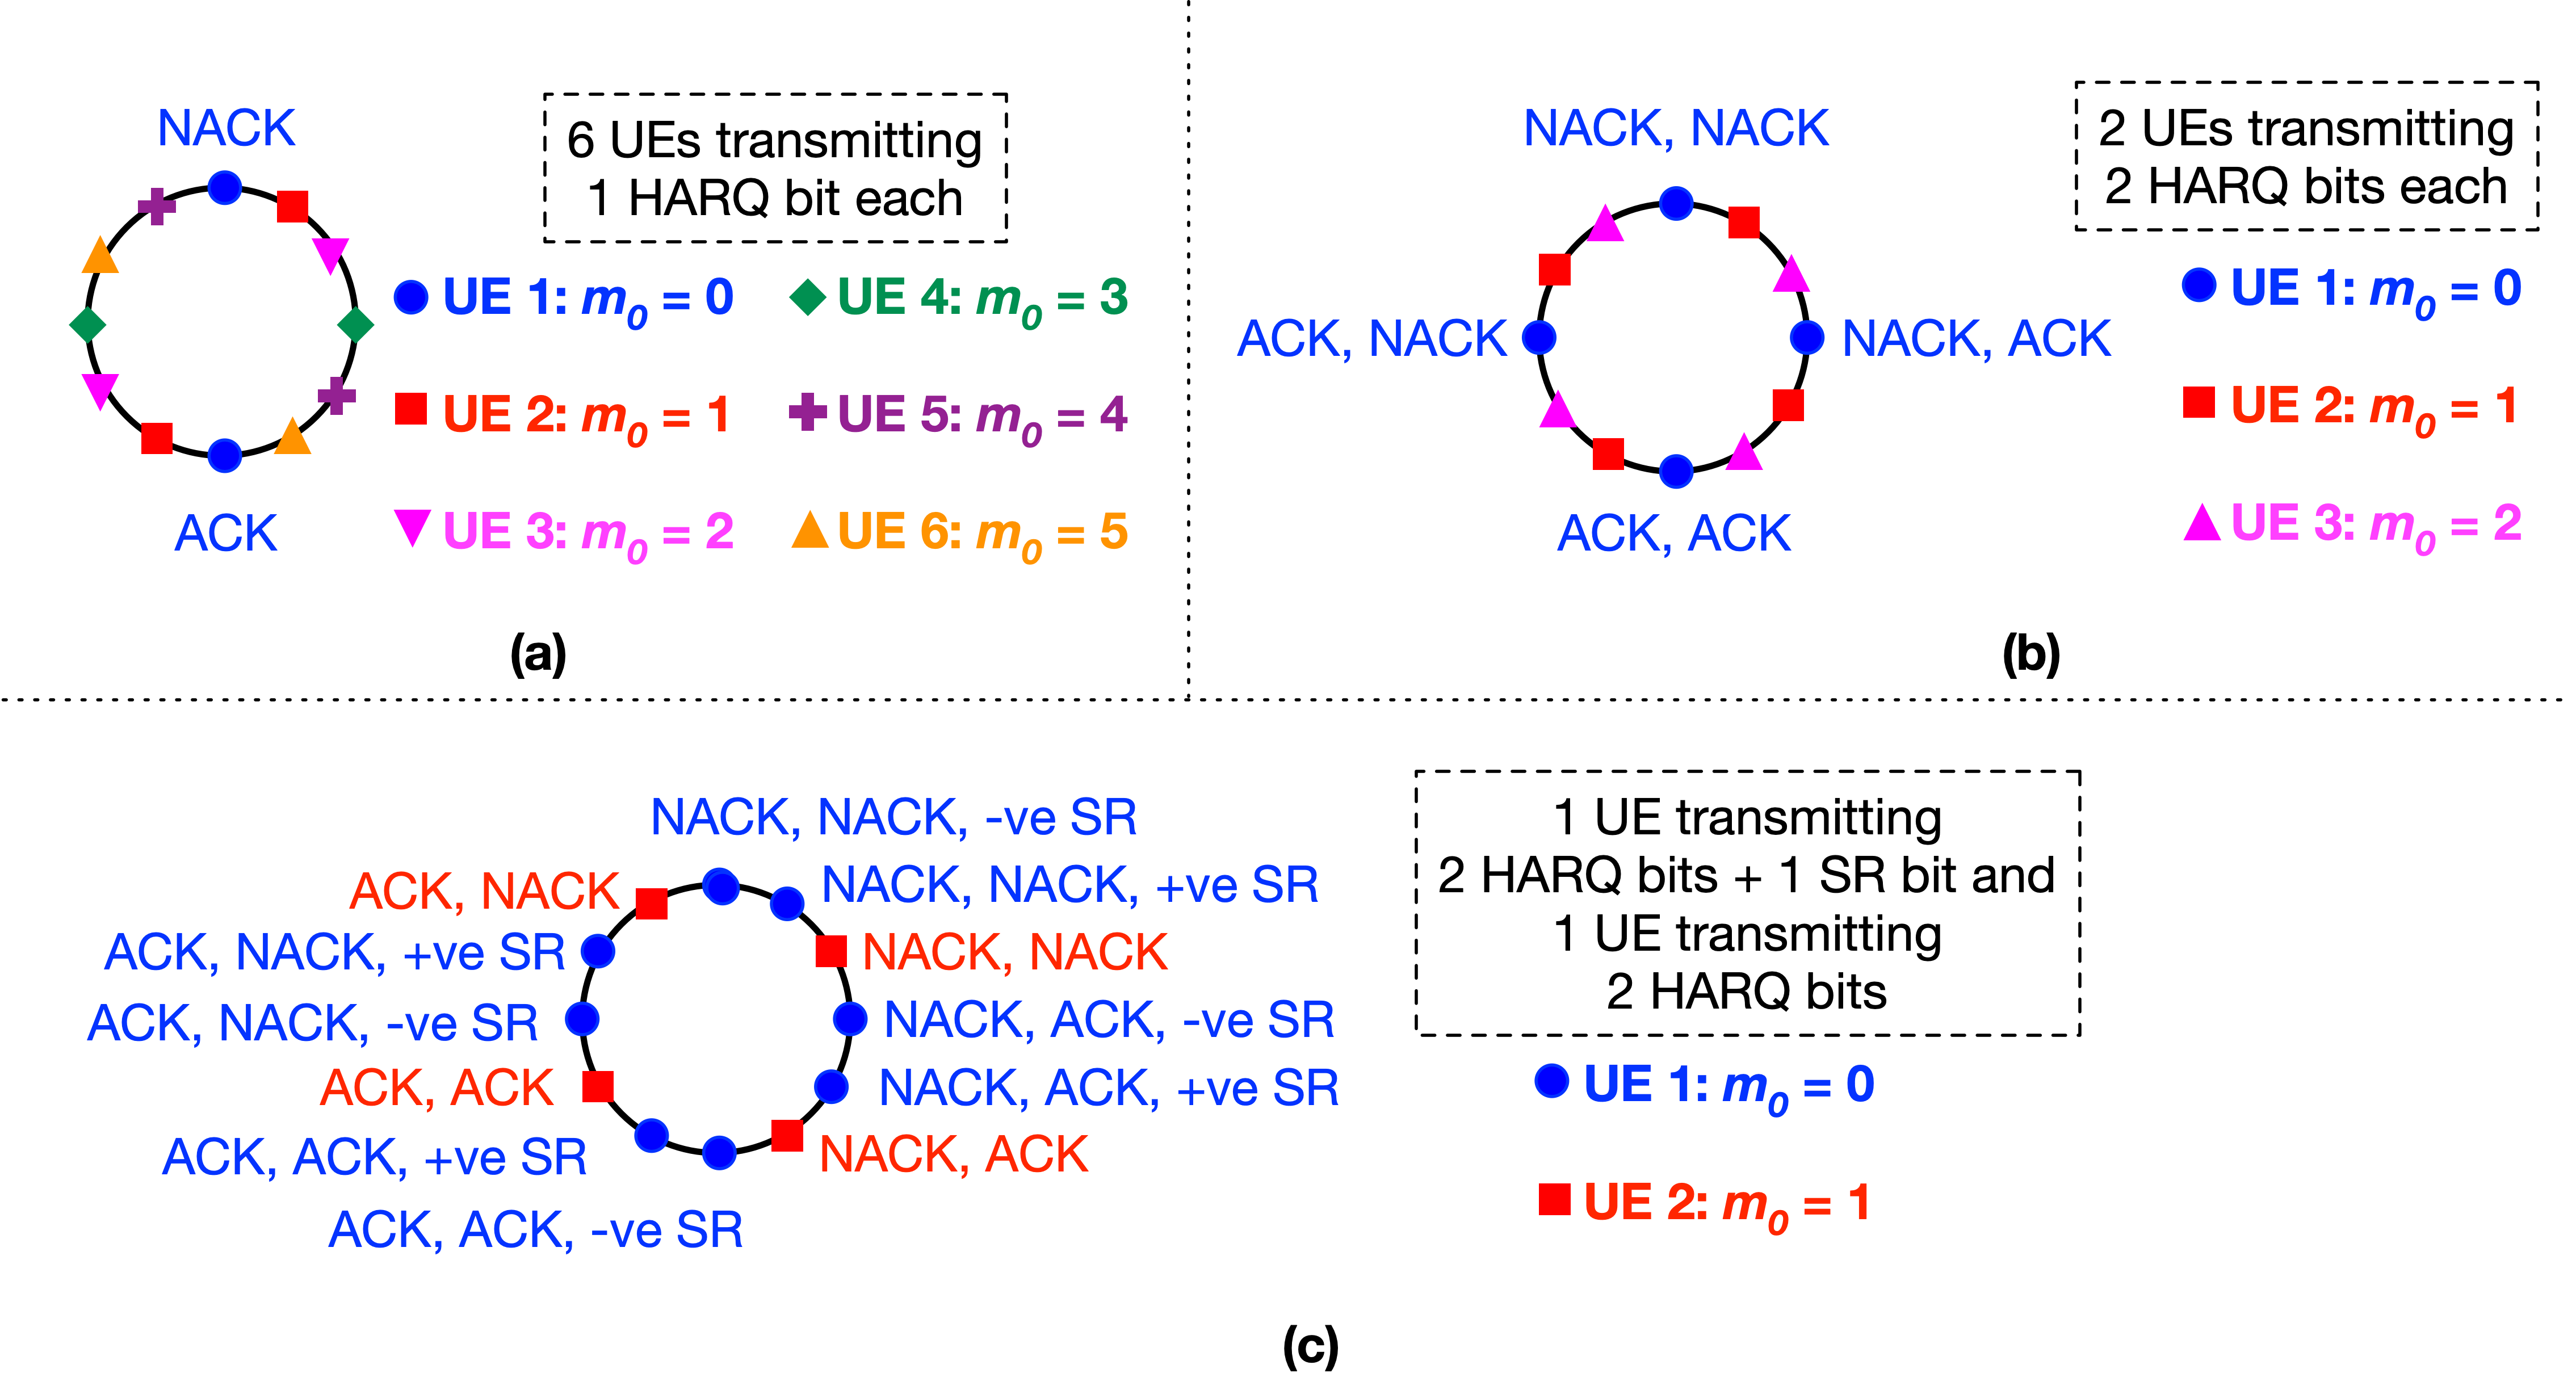
\includegraphics[width=0.48\textwidth]{Figures/m_cs_table_v3.png}
    \caption{Example scenarios showing how assigning different initial cyclic shifts to different UEs allows them to be multiplexed on the same time-frequency resources.}
    \label{fig: m_cs_mux_ue}
\end{figure} 

Accounting for UE multiplexing, the generalized multi-user Format 0 received signal in the frequency domain is given by,

\begin{equation}
    y(k) = \sum_{m = 0}^{N_{UE}-1}h_{m}(k)e^{j\alpha_{m} k}\cdot\bar{r}_{u,v} (k) + w(k),
    \label{eq: pucch_rx_signal}
\end{equation}
where $k = 0,1,2,..., N_{sc}^{RB}-1$, $N_{UE}$ is the number of multiplexed UEs in a given resource block, $h_{m}(k)$ is the channel between the gNB and the UE transmitting the base sequence with cyclic shift $\alpha_m$ in the $k^{th}$ Resource Element (observe that all multiplexed UEs use the same base sequence). The noise is denoted by $w(k)$.

% \subsection{PUCCH FORMAT 0 PERFORMANCE METRICS}
% Literature mentions several performance metrics like Discontinuous Transmission(DTX), False Detection, and Missed Detection~\cite{9691557} to evaluate the performance of PUCCH Format 0 decoding. 

% i) If the receiver does not detect any transmission on a HARQ resource, it is marked as DTX. This could be a result of a failure to detect a prior Downlink message at the UE or a failure in detecting the acknowledgment at the gNB receiver. 

% ii) False detection means that one or more UEs have not actually transmitted on the PUCCH resource but the receiver wrongly identifies it as a true transmission and decodes false UCI bits.

% iii) Missed detection means that one or more UEs have transmitted on the PUCCH and the receiver wrongly decodes the UCI bits.

%  It is obvious that incorrect detection of SR bits when there are none will cause the gNB to allocate a large chunk of unnecessary uplink resources to one or more UEs.  Incorrect detection of HARQ bits will either cause unnecessary re-transmissions or the lack of re-transmissions even when decoding of downlink transmissions has failed. Several wrong detections of SR and/or HARQ bits reduce the throughput and reliability of the wireless link. As a result, it is the goal of any receiver algorithm, conventional or AI/ML to minimize the probability of missed and false detections. In later sections, we compare the performance of our NN based receiver with both the DFT based receiver as well as 3GPP conformance requirements~\cite{3gpp_38_141}.

% Two types of metrics emerge. Missed detection and false detection. Missed detection means that one or more UEs have transmitted on the PUCCH and the receiver wrongly decodes the UCI bits. False detection means that one or more UEs have not actually transmitted on the PUCCH but the receiver wrongly identifies it as a true transmission and decodes false UCI bits. It is obvious that incorrect detection of SR bits when there are none will cause the gNB to allocate a large chunk of unnecessary uplink resources to one or more UEs.  Incorrect detection of HARQ bits will either cause unnecessary re-transmissions or the lack of re-transmissions even when decoding of downlink transmissions has failed. Several wrong detections of SR and/or HARQ bits reduce the throughput and reliability of the wireless link. As a result, it is the goal of any receiver algorithm, conventional or AI/ML to minimize the probability of missed and false detections. In later sections, we compare the performance of our NN based receiver with both the DFT based receiver as well as 3GPP conformance requirements~\cite{3gpp_38_141}.

\subsection{Existing Methods For PUCCH Format 0}

\subsubsection{Conventional Approaches}
We reiterate that Format 0 has no provision for DMRS (pilots), and hence, there is no channel estimation or equalization possible. Blind correlation methods~\cite{1261943}~\cite{4595664} exist for such scenarios in which channel information is unknown, but these methods are often reserved for scenarios in which the resource allocation information is also not known. One example of such a scenario is the initial time synchronization between the gNB and the UE. Since the allocation of the synchronization sequences is unknown, longer correlations need to be performed. But, by the time the first Format 0 signal is received at the gNB, time and frequency synchronization are already achieved, and the gNB is aware of the UE's transmission~\cite{wahlqvist1996time}. Since the allocation is known and is always 1 RB long, a simpler length 12 correlation is sufficient.

In ~\cite{kim2020performance, tadavarty2021performance, phan2021enhanced}, various receiver techniques based on correlation are considered. Correlation relies on the fact that the low PAPR base sequence used for encoding the UCI content is known at the receiver. The decoding method involves correlating the received samples with various cyclically shifted versions of the base sequence. The predicted cyclic shift is the cyclic shift that gives the highest correlation magnitude. It should be noted that peak selection, by definition, requires an optimal threshold for determining whether a peak is due to noise or a true transmission.  

The work in~\cite{kim2020performance} shows that correlation-based signal detection outperforms methods based on raw signal power measurements even under fading channel scenarios. A normalized correlation-based solution for identifying false detections of HARQ bits is provided in~\cite{tadavarty2021performance}. The solution uses the probability distributions of a normalized correlation peak to determine the optimum threshold for classifying a reception as false. The PUCCH format 0 receiver algorithm proposed in~\cite{phan2021enhanced} eliminates phase opposition across multiple hops by finding the sum of correlation magnitudes across symbols instead of correlation values. 

In the 5G testbed deployment at IIT Madras~\cite{5gtbiitm}, the correlation is implemented by an equivalent DFT-based algorithm. Later in the paper, we use this as a baseline for comparison. Such an algorithm proves to be better from a hardware perspective due to its optimized use of resources (avoiding the need to correlate with all the shifted base sequences), reduced latency, and higher throughput. In the IIT Madras 5G testbed, a DFT-based receiver for PUCCH Format 0 has been implemented on custom Field Programmable Gate Array (FPGA) boards for real-time operations.
\begin{figure}[h]
    \captionsetup{justification=justified}
     \centering
     \begin{subfigure}[b]{0.48\textwidth}
         \centering
         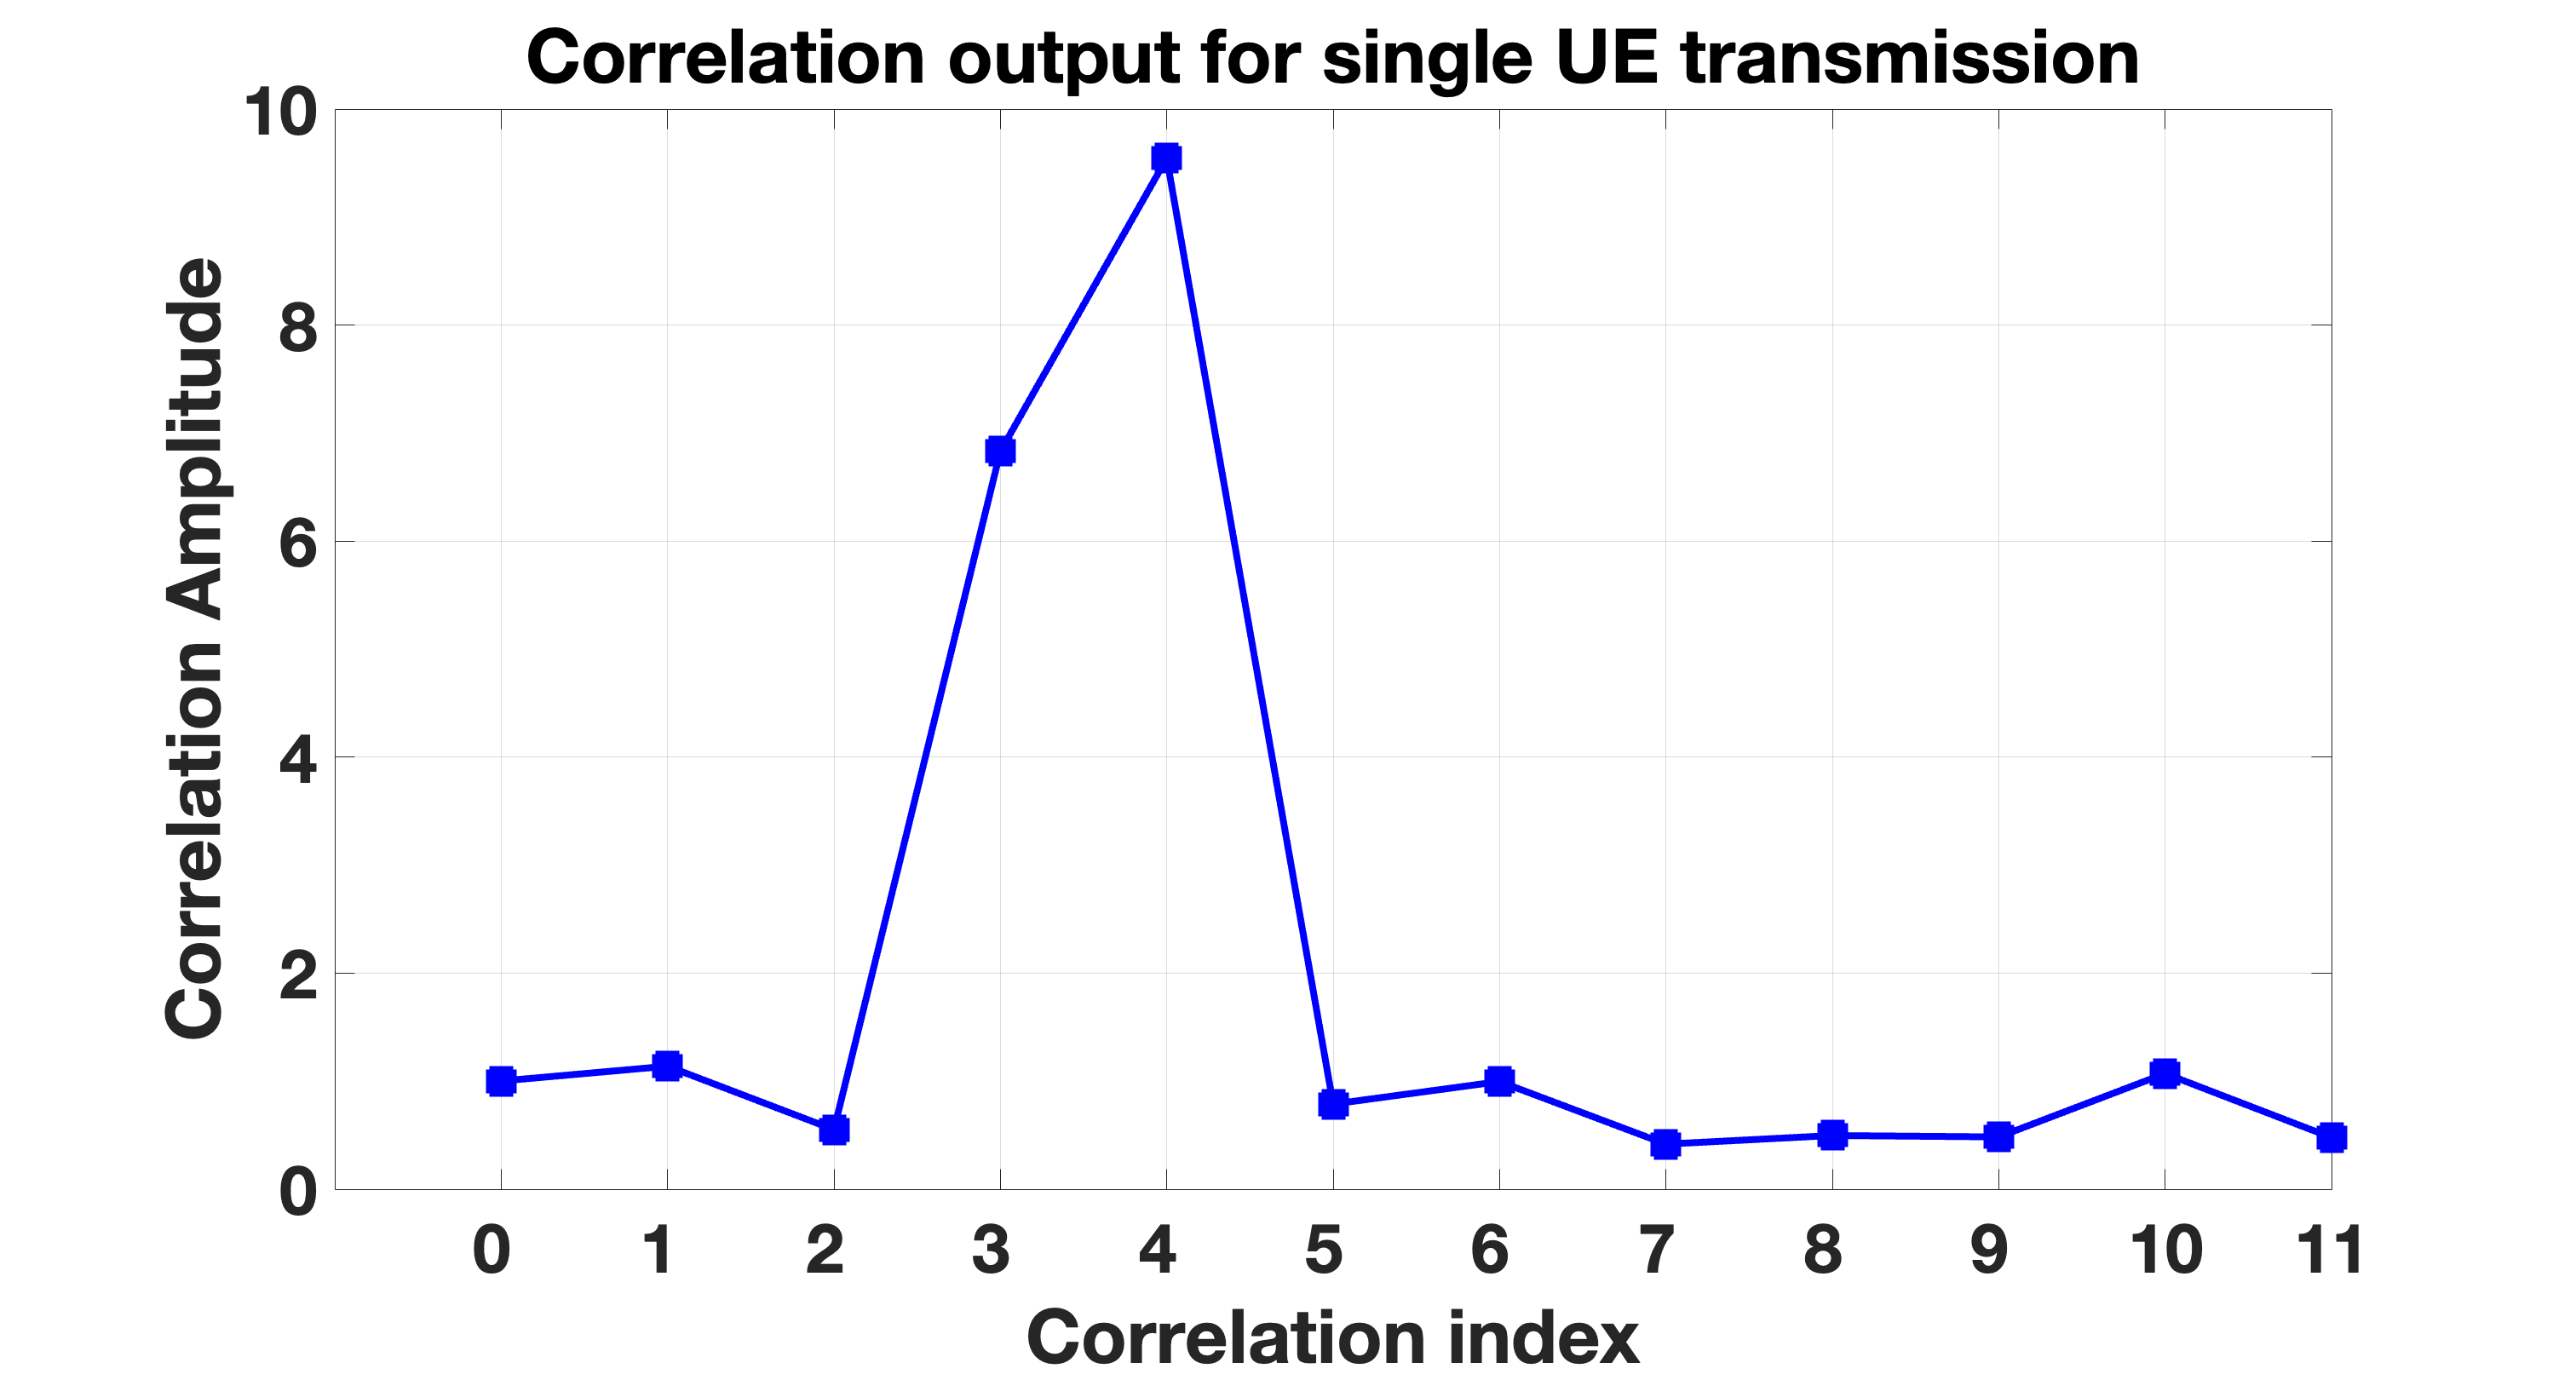
\includegraphics[width=\textwidth]{Figures/correlation_1_ue.png}
         \caption{}
         \label{fig: correlation_1_ue}
     \end{subfigure}
     \\
     \begin{subfigure}[b]{0.48\textwidth}
         \centering
         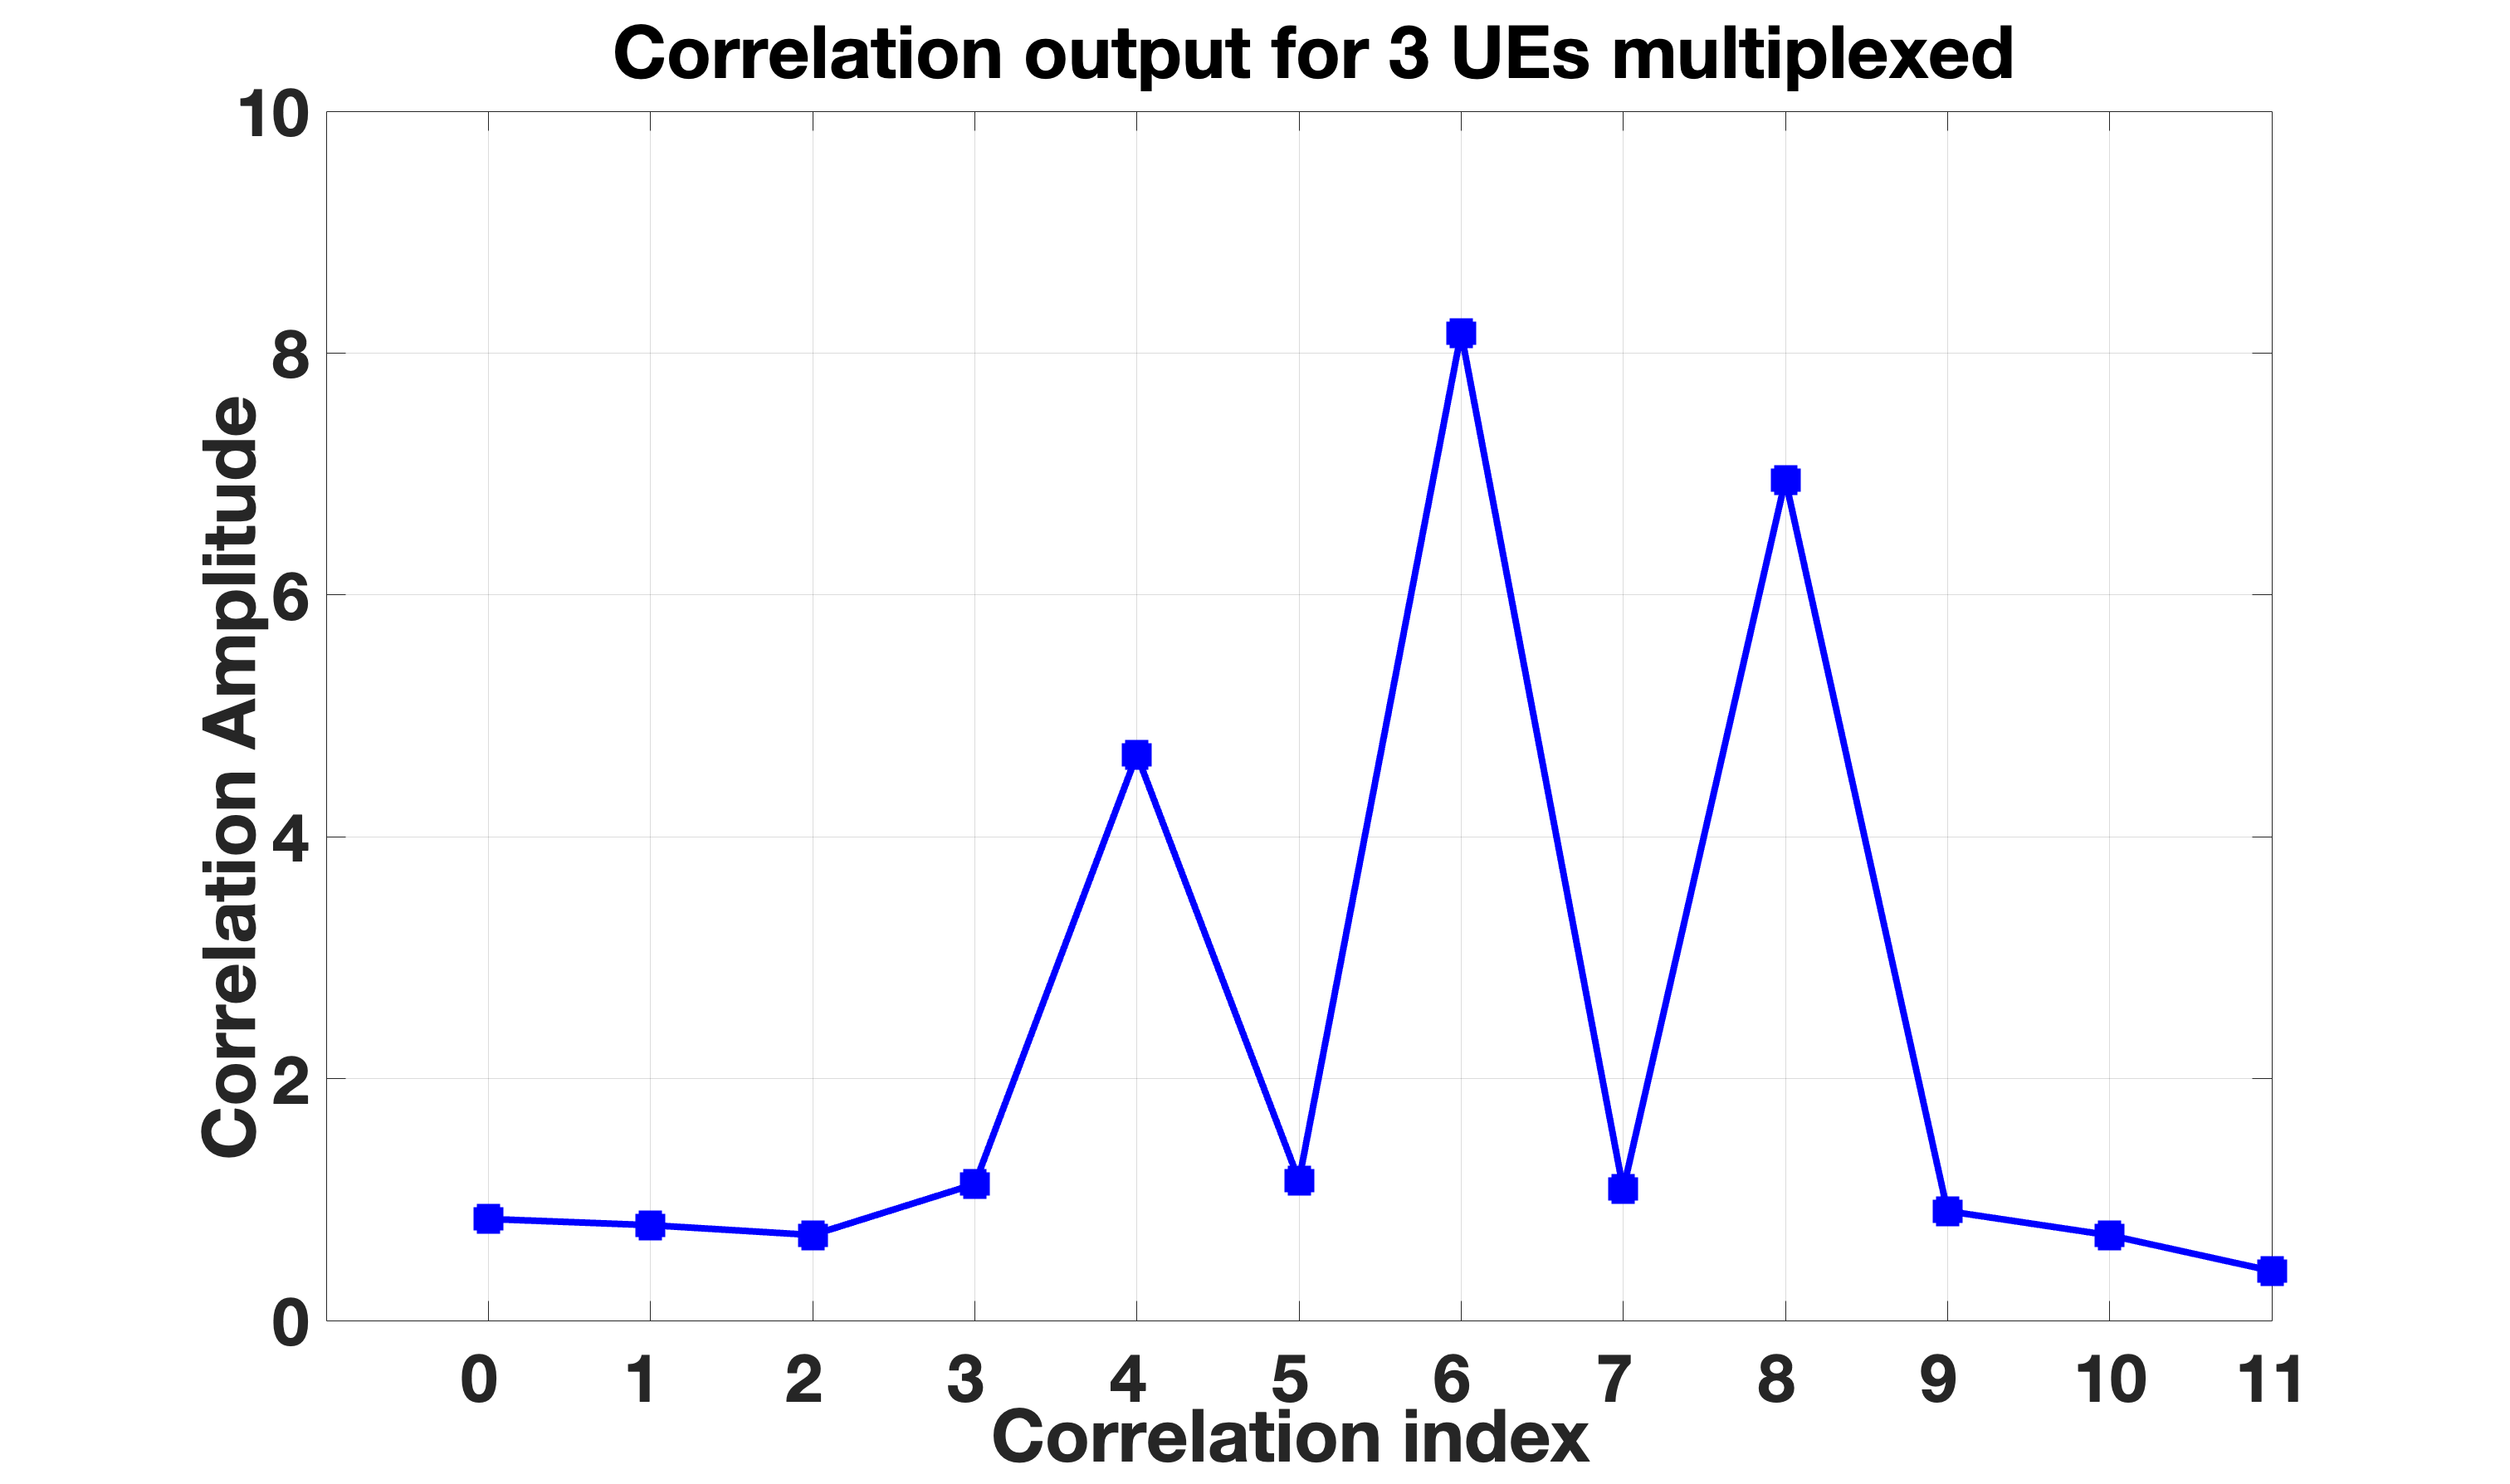
\includegraphics[width=\textwidth]{Figures/correlation_3_ue.png}
         \caption{}
         \label{fig: correlation_3_ue}
     \end{subfigure}
        \caption{Illustration of the output of Correlation of received Format 0 signal with the known base sequence for (a) 1 UE transmission and (b) 3 UEs multiplexed transmission}
        \label{fig: correlation_plots}
\end{figure}
This method recovers the phase rotation $\alpha$ by taking the 12-point DFT of $y(n)\cdot \bar{r}^{*}_{u,v} (n)$. Since $y(n)=e^{j \alpha n}\cdot \bar{r}_{u,v}(n)$, the multiplication of the base sequence $\bar{r}_{u,v}$ with its complex conjugate forces it to unity. The 12-point DFT of the resultant exponential term $e^{j \alpha n}$ results in a peak at $\alpha$. This is shown in Figure~\ref{fig: correlation_1_ue} with a correlation peak at $index = 4$. The correlation index corresponding to the maximum correlation amplitude is taken as the estimated $\alpha$ value. Recall from~\eqref{eq: alpha} that $\alpha$ is a combination of $m_{0}$, $m_{cs}$ and $n_{cs}$. Therefore, upon the subtraction of $m_{0} + n_{cs}$ from $\alpha$ (subtraction is modulo 12), the UCI-specific cyclic shift $m_{cs}$ remains. In scenarios where multiple users ($N_{UE}$ of them) transmit PUCCH Format 0 signals in the same time-frequency location, the DFT algorithm selects the top $N_{UE}$ peaks from the DFT output and uses them to determine the $m_{cs}$ for each of the $N_{UE}$ multiplexed UEs. Figure~\ref{fig: correlation_3_ue} shows an example in which 3 UEs are multiplexed. In this case, we select the top 3 peaks (at $index = 4, 6,$ and $8$) as $\alpha$ values. 

We observe that while the above works in literature do provide false and missed detection performance analysis, they are based on fixed thresholds that are specific to a certain scenario and derived from lengthy Monte Carlo simulations. Another significant element that is not considered in~\cite{kim2020performance, tadavarty2021performance, phan2021enhanced} and considered only to some extent in~\cite{5gtbiitm} is the multiplexing of multiple UEs in the same resources. 

It is not clear how the thresholds in the above work and implementations extend to multiplexed UEs. Furthermore, fixed thresholds do not account for the received signal power variations that are caused due to variations in gains of hardware elements such as the LNA and due to varying locations of the multiplexed UEs. For example, a true transmission with large distance-based path loss could be misclassified as false if a fixed threshold is used.

Finding a one-size-fits-all threshold for various channel environments and multiplexed UEs is non-trivial. This has led us to explore an AI/ML-based data-driven approach in which a receiver could be designed directly from the raw frequency domain signals rather than correlation values. We apply similar techniques here. The IQ samples in the received resource block are analogous to pixel values in an image. Hence, models that work for image classification could potentially work here too.

\subsubsection{AI/ML Approaches}
To our knowledge, there is limited work on applying AI/ML toward the decoding of Format 0 signals. One of the first models for Format 0 decoding was proposed in our previous work~\cite{yerrapragada2023machine}. However, this was an initial effort that focused on training the model to predict 1 out of 4 possible $m_{cs}$ values in the specific case of 1 HARQ + 1 SR transmission. The architecture described in this paper extends our previous work to support all the possible UCI payloads shown in Table~\ref{tab: pucch_summary} and all the possible multiplexing combinations of UEs ($N_{UE} = 0, 1, \dots, 12$). This generalized architecture is designed for potential field deployment in any 5G gNB.

\section{Machine Learning Receiver For PUCCH Format 0 Detection}
This section lays down the framework for posing the PUCCH Format 0 detection as an AI/ML classification problem. Specifically, we show how a single multi-label neural network classifier can serve as a generalized PUCCH Format 0 decoder. 

\subsection{PUCCH Format 0 as an AI/ML Classification Problem}
Classification, a widespread use case of machine learning algorithms, is a supervised learning task that involves identifying to which class (label) a given data instance belongs. A predictive model, typically a Neural Network, is trained with a dataset that contains several input instances and the corresponding ground truth class labels. Labeled data helps us "supervise" the NN in learning the correct input-output mapping. 

Learning happens by iteratively minimizing a loss function, which is a distance metric between the predicted label and the ground truth label. In many classification tasks, the input-output mappings are intractable. ML techniques, such as Neural Networks, have proven to be more adept at extracting these mappings. 

There are typically three types of classification tasks. The first is Binary Classification, in which the input data falls into one of two classes. An example of this is email classification as spam or not spam. The second is multi-class classification, in which input data could belong to one of more than two classes. A routinely cited example is classifying handwritten digit images into one of ten numbers. The third is multi-label classification, in which input data can independently belong to more than one class. An example of this is the identification of multiple genres a movie belongs to, given a summary of its plot. 

For PUCCH Format 0, the classification task is as follows: Given a sequence of received frequency domain Format 0 samples, predict the $N_{UE}$ phase rotation values $\alpha_{0}, \alpha_{1} \dots \alpha_{N_{UE}-1} $ (see Eq.~\eqref{eq: pucch_rx_signal}) applied to the base sequence. The obtained $\alpha$ values can then be mapped back to the UCI-specific cyclic shift $m_{cs}$ for each UE by modulo 12 subtraction of the corresponding $m_{0}$ and $n_{cs}$ which are provided by the higher layers (L2). 
In the case where no user is transmitting on the PUCCH ($N_{UE} = 0$), the NN prediction has to reflect this. In summary, the NN classifier has to predict either a single $\alpha$ value, multiple $\alpha$ values, or zero $\alpha$ values. Such a pattern of prediction is a typical use case of multi-label classification. 

\subsection{Data Generation And Representation}
Dataset generation in AI/ML for wireless communication has a unique challenge not present in other domains - the non-availability of off-the-shelf benchmark datasets. One way of developing such datasets is through state-of-the-art simulation tools, such as the MATLAB 5G Toolbox, which can generate near-accurate datasets under various channel impairments. Simulated data is a good starting point for training neural networks in communication problems. However, we note that including field data, if available, gives us an insight into the generalization performance of AI/ML models across different distributions of data. The inclusion of field data also aligns with 3GPP requirements for 5G Release 18~\cite{3gpp_38_843}. For this paper, we use a combination of the above two approaches for data generation. The datasets used in this paper are publicly available at ~\cite{aiml_pucch_dataset}.

\subsubsection{Simulated Datasets} 
Using the MATLAB 5G Toolbox, we generate the received waveforms containing the PUCCH Format 0 signals. These generated waveforms include fading channel impairments and Additive White Gaussian Noise (AWGN). For various SNR values ($0$, $5$, $10$, $15$, and $20$ dB), we generate PUCCH signals transmitted over a TDL-C Channel and store the noisy received samples. These samples are the input to the NN. For each input, the corresponding output label is the applied phase rotation $\alpha$ for each of the $N_{UE}$ UEs in multi-hot encoded format. 

The pseudocode for generating PUCCH Format 0 datasets in MATLAB is shown in Algorithm~\ref{alg: data_gen}. We first place PUCCH Format 0 signals on all 14 symbols in a slot and 12 resource blocks in each symbol spaced 20 resource blocks apart. This results in 168 allocations per resource grid. We generate 1000 iterations of such resource grids. These 1000 grids are generated for each value of $N_{UE}$ in the range 0 to 12. The process is further repeated for the five SNR values.  

\begin{algorithm}[h]
    \caption{Training dataset generation}
    \label{alg: data_gen}
    $\operatorname{N_{UE}} = \{0, 1, 2, \dots, 12\}$ \\
    $\operatorname{SNR} = \{0, 5, 10, 15, 20\}$ dB \\
    $\operatorname{Iter} = \{1, 2, \dots, 1000$\} \\
    \ForEach{$\operatorname{N_{UE}}$, $\operatorname{SNR}$, $\operatorname{Iter}$}{
        $\operatorname{n_{UE}} = 0, 1, 2, \dots, \operatorname{N_{UE}}$ \\
        \ForEach{$u \in \operatorname{n_{UE}}$}{
            \ForEach{$c \in \{1, 2, \dots, 168\}$}{
                bit\_len\_harq $\in \{0, 1, 2\}$ \\
                bit\_len\_sr $\in \{0, 1\}$ \\
                Generate UCI bits and label ($\alpha$) \\
                Generate Format 0 signal and place it in the resource grid\\
                }
            OFDM Modulation of the TX OFDM grid\\
            Transmit over channel
        }
        Receive combined signal from $\operatorname{N_{UE}}$ UEs (Eq.~\ref{eq: pucch_rx_signal})\\
        Perform OFDM Demodulation to obtain the RX grid\\
        \ForEach{$c \in \{1, 2, \dots, 168\}$}{
            Extract and save Format 0 signal \\
        }        
    }
\end{algorithm}


\subsubsection{Real-Time Over-The-Air Datasets}
We use hardware captures derived from the state-of-the-art 5G testbed at IIT Madras~\cite{5gtbiitm} for more realistic testing. The hardware captures help represent channel states and hardware impairments not included in the training dataset. The setup (see Figure~\ref{fig: hw_setup}) consists of an N5182B Vector Signal Generator (VSG) for transmitting the  5G signal at a center frequency of $3.49986$ GHz (one of the sub-6 GHz channel raster in the n78 band). In our setup, the VSG acts like a UE, and it uses a commercial omnidirectional wideband monopole antenna to transmit the signals. The VSG is connected to the antenna through 2 SMA cables with $1.9$ dB wire loss each. Here, commercial UEs could not be used because it is not easy to extract the actual transmitted information, i.e., ground truth labels for the UCI transmissions made by the UE. Also, the dynamic nature of the allocations made by the L2 scheduler makes it difficult to capture the data at the gNB for that particular time duration.

A  multi-channel 5G Remote Radio Head (RRH) with a dual-polarized antenna at the gNB receives the signals from over the air (for the purpose of the paper, we utilize only one antenna and one transceiver chain). The RRH operates in the n78 band with $100$ MHz bandwidth. It is ORAN-compliant and follows the 7.2b split as defined in~\cite{ORAN_spec}. Other receiver components of the RRH include an in-house Low Noise Amplifier (LNA) with 60dB gain at the receiver front end and an ADRV 9009 RF transceiver. We place the transmitter antenna one meter away from the receiver. The PUCCH Format 0 signal is transmitted from the VSG through an antenna, over the air, and then received at the RRH antenna, followed by the LNA and the transceiver. The signal out of the 16-bit ADC is then collected and used for testing. 

\begin{figure}[h]
\centering
\includegraphics[width=0.35\textwidth]{Figures/hw_setup.png}
\caption{IIT-Madras 5G testbed setup with the Remote Radio Head used as a receiver (gNB) and the VSG used as a transmitter (Emulated UE).}
\label{fig: hw_setup}
\end{figure}

\begin{figure*}[t!]
\centering
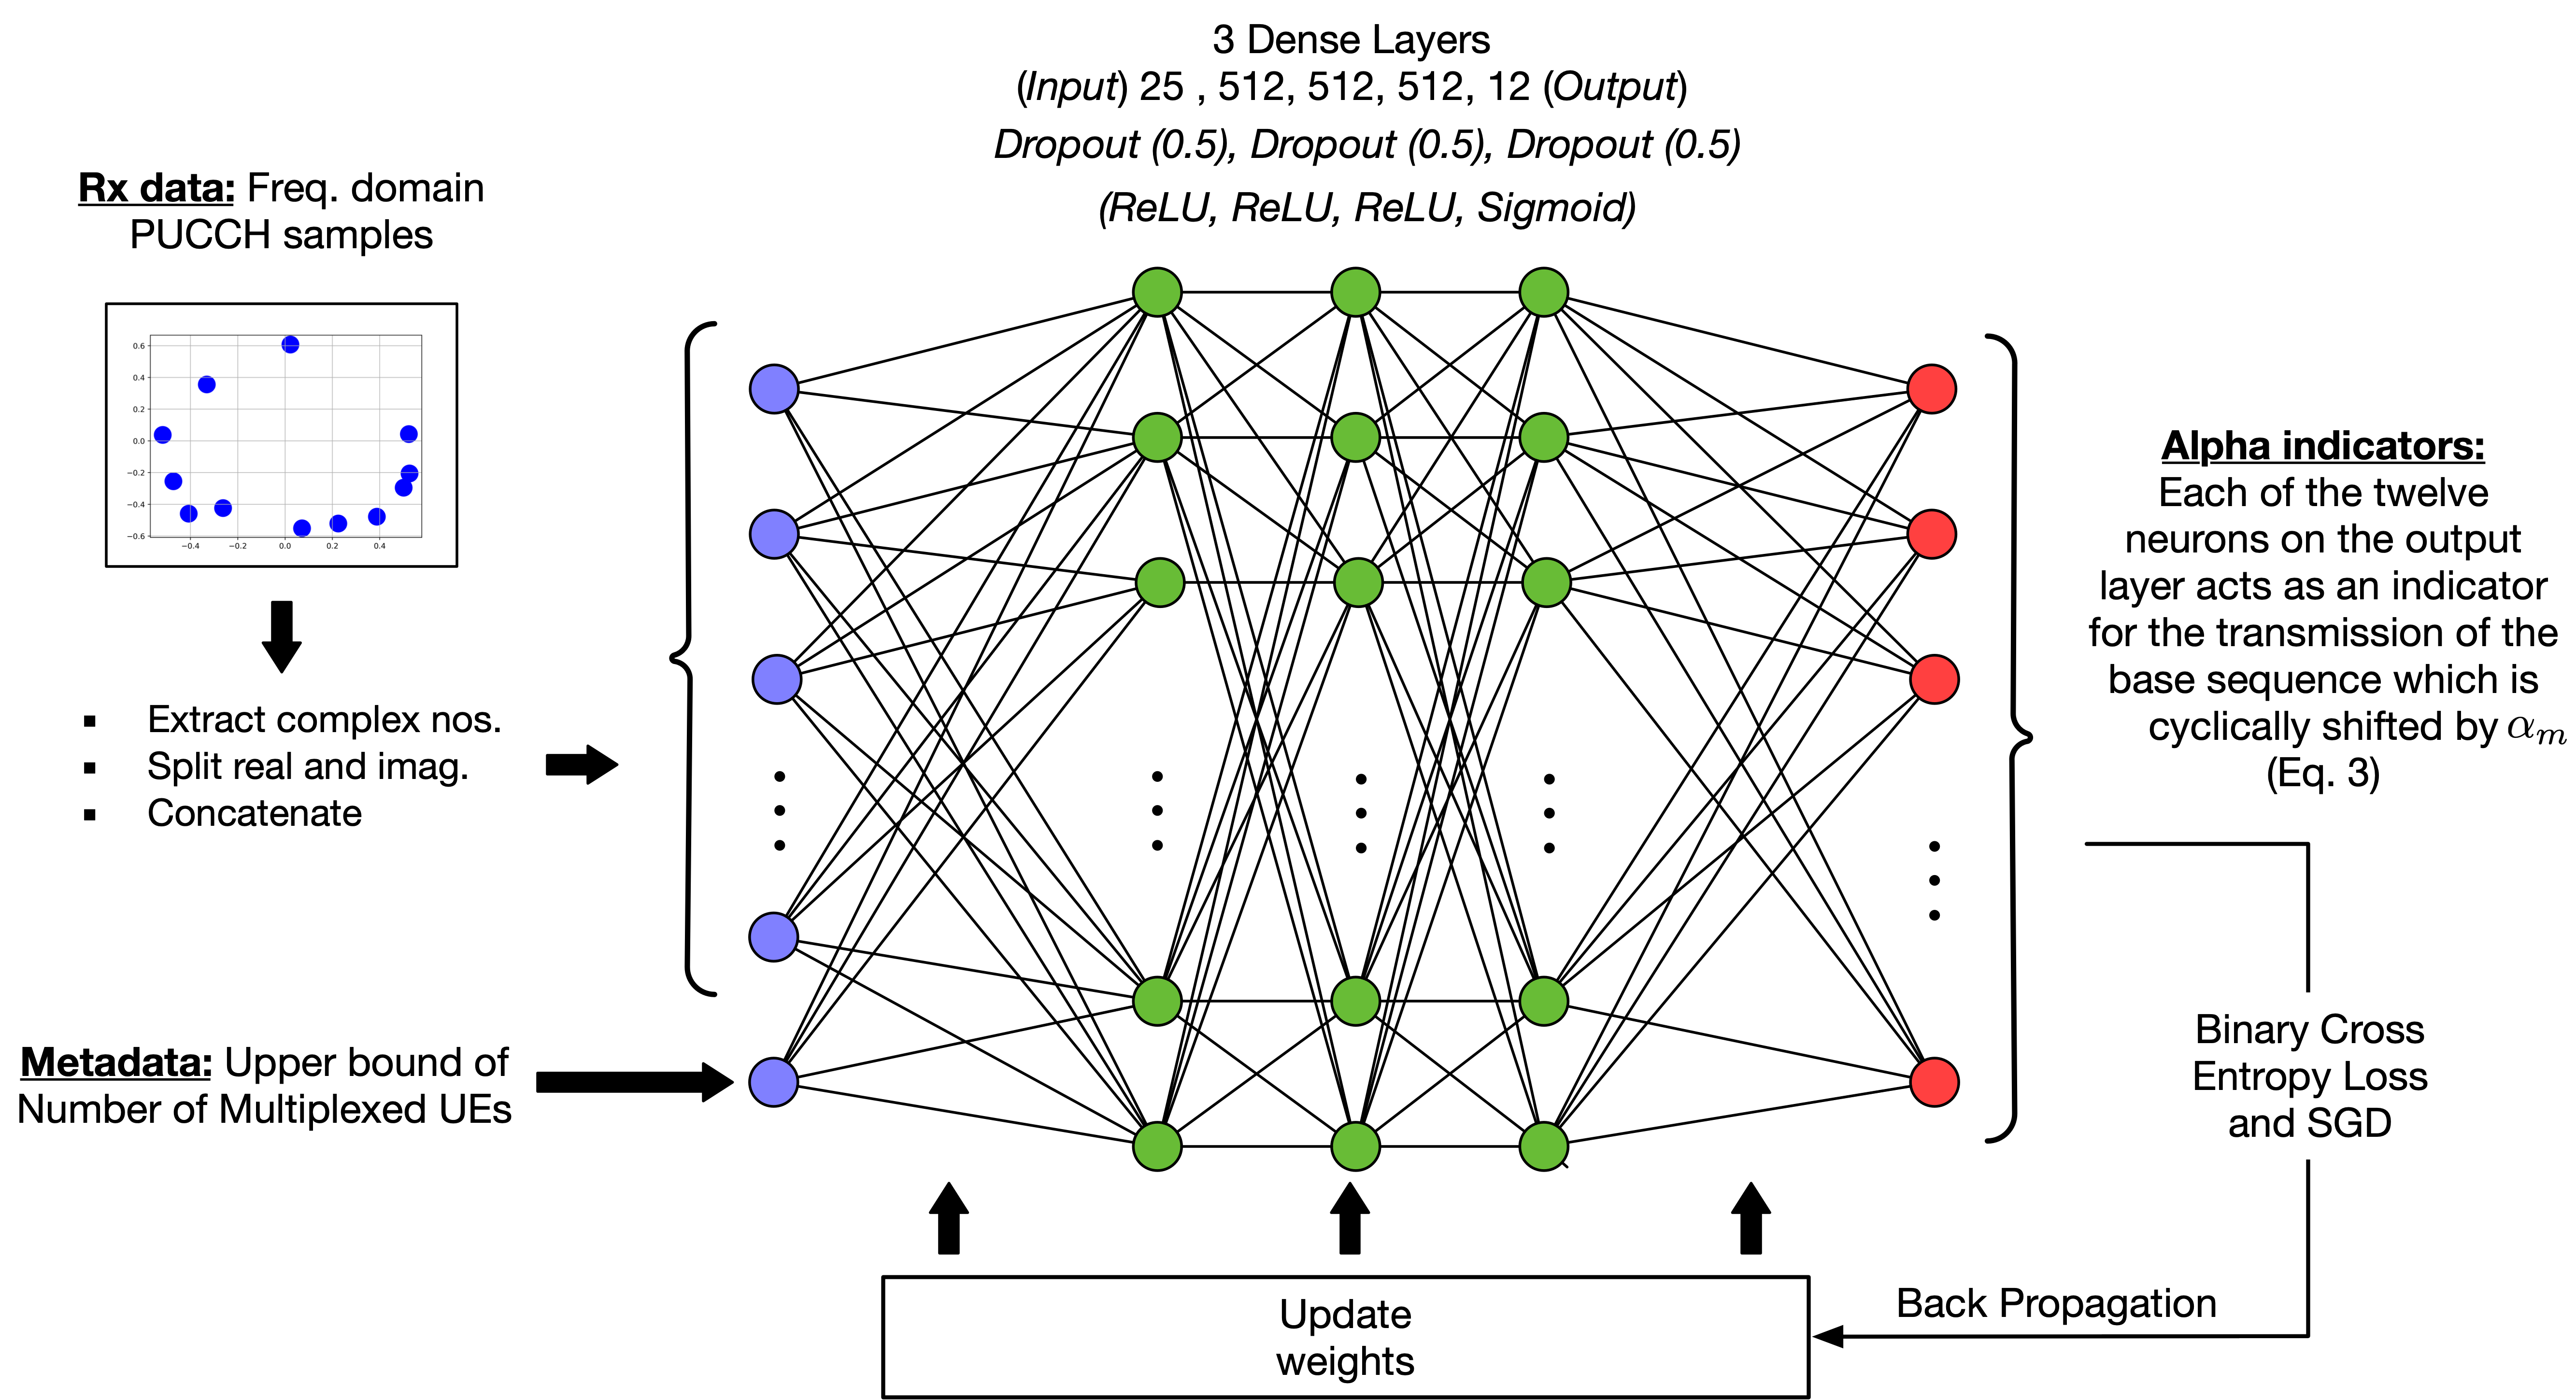
\includegraphics[width=0.9\textwidth]{Figures/3L_pucch_single_nn_framework.png}
\caption{UCINet0 Architecture for PUCCH Format 0 decoding with 25 neurons in the input layer, 512 neurons in each of the three hidden layers and 12 neurons in the output layer.}

\label{fig: nn_arch}
\end{figure*}

\subsection{Neural Network Architecture}
Given a problem statement, there is no formula for knowing apriori, the best neural network architecture. For most problems, initial architectures are determined based on prior experience and domain knowledge. These architectures are then tuned by experiment. Figure~\ref{fig: nn_arch} shows the UCINet0 architecture that showed the best performance in our experiments. In subsequent sections, we also comment on the trade-off between high complexity and performance.

\subsubsection{Neural Network Structure}
The input to the NN has two components. The first is the received PUCCH Format 0 signal, and the second is metadata indicating the number of multiplexed UEs that the receiver expects. Since the PUCCH Format 0 signals occupy a single Resource Block, there are 12 received complex samples. We separate the real and imaginary parts of each complex number and concatenate them, resulting in a length 24 real sequence. As shown in Eq.~\eqref{eq: pucch_rx_signal}, a given PUCCH resource block at the receiver could contain the sum of signals from multiple UEs. To aid the neural network, we also feed the number of multiplexed UEs as a 25th metadata input. The number of multiplexed UEs that a receiver should expect to see is often provided by an L2 scheduler as an upper bound, meaning that the received signal could contain less than or equal to the number of UEs indicated by L2. We denote the difference between the actual number of UEs multiplexed and the number of UEs indicated by L2 as $\Delta$. One example of a scenario where this is observed is when the L2 scheduler allocates multiple UEs to transmit SR, but not all of the UEs have any data to transmit. In such cases, UEs that do not require PUSCH resources do not transmit the SR.

\begin{figure}[h!]
    \centering
    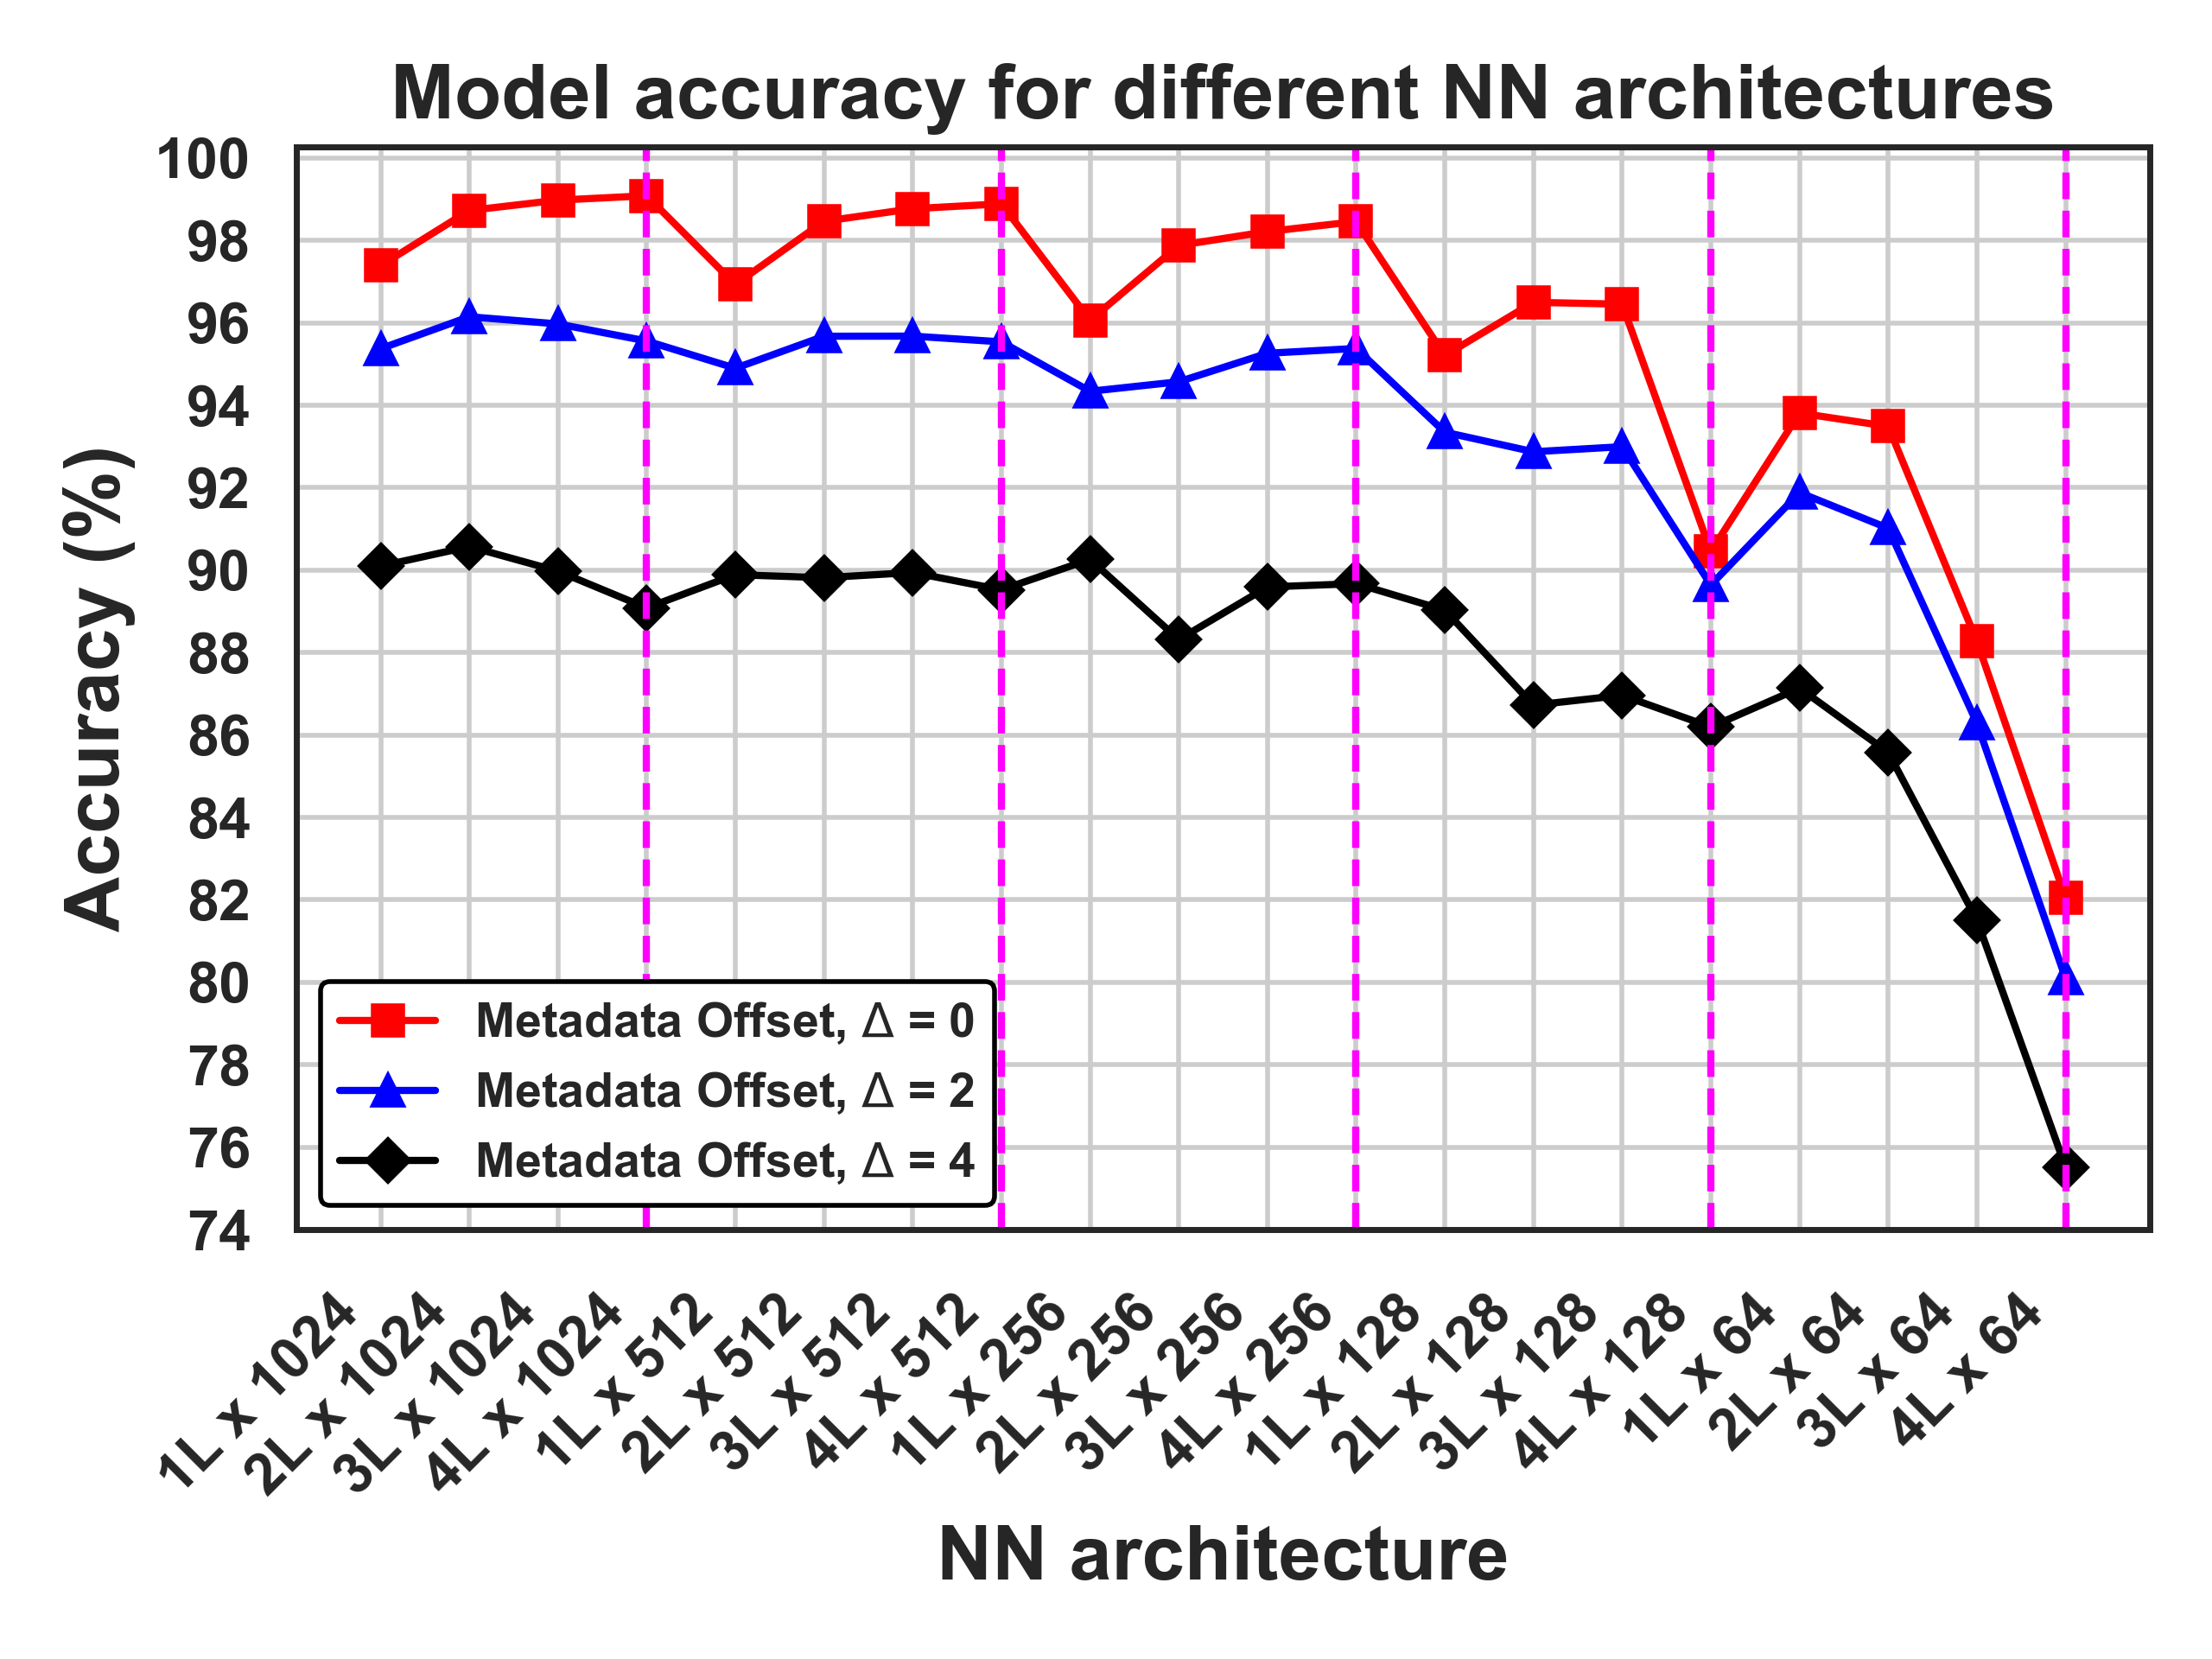
\includegraphics[width=0.48\textwidth]{Figures/Hw_complexity_analysis_all_arch_epochs_150.png}
    \caption{Model accuracy for different FCN architectures at various values of $\Delta$. Here, $\Delta$ represents the maximum metadata offset between the true value and L2’s upper bound for the number of multiplexed UEs. We use these results to arrive at the final UCINet0 architecture presented in this paper.}
    \label{fig: acc_vs_complexity}
\end{figure}
Owing to the relatively small dimension of the input, our proposed UCINet0 is a Fully Connected Neural Network (FCN). As shown in Figure~\ref{fig: nn_arch}, there are 3 dense layers, each containing 512 neurons. 
The output layer contains twelve neurons. Each output neuron acts as an indicator for the transmission of the base sequence which is cyclically shifted by $\alpha_m$~\ref{eq: pucch_rx_signal}. We arrived at the final UCINet0 architecture of 3 layers and 512 neurons after having evaluated the performance of other architectures with a varying number of layers and neurons. Figure~\ref{fig: acc_vs_complexity} shows the UCI decoding accuracies(defined in IV~\ref{subsec: accuracy}) obtained with 20 variations of FCN architectures. We considered combinations of $1$, $2$, $3$ and $4$ layer models with $64$, $128$, $256$, $512$ and $1024$ neurons. 

From Figure~\ref{fig: acc_vs_complexity}, we observe the following: 

\begin{itemize}
    \item Model performance generally improves as we increase the number of neurons from $64$ to $1024$ for any number of layers and for values all of $\Delta$.
    \item For $\Delta=0$, both $1024$ and $512$ neurons result in almost the same accuracy values for a given number of layers. For example, $2 \text{ layers} \times 1024$ and $2 \text{ layers} \times 512$ result in similar accuracy values.
    \item For higher values of $\Delta$, the accuracy drops as the number of layers increases beyond a certain value as the model begins to overfit. For $\Delta=4$ and $1024$ neurons, the accuracy drops beyond 2 layers, whereas for $512$ neurons, the accuracy drops beyond 3 layers.
\end{itemize} 

 Hence, considering the balance between the number of layers, number of neurons, and accuracies for various $\Delta$ values, 3 layers with $512$ neurons architecture seems to be the optimal choice.
 
\subsubsection{Dropout}
Dropout~\cite{srivastava2014dropout} is used during training to "drop out" or cut off certain neurons and their connections randomly with a certain probability during training. It serves two purposes - Ensemble Learning~\cite{hara2016analysis} and Regularization~\cite{Goodfellow-et-al-2016}. Ensemble learning helps improve predictive performance by combining the outputs of multiple AI/ML models or multiple instances of the same AI/ML model trained on different subsets of data. However, training a large number of models is extremely prohibitive both in terms of time and computational resources. With dropout, in each backward pass, only a subset of weights are updated, effectively resulting in a new neural network. The subset of weights that are updated varies with each forward and backward pass, thus creating the combined effect of training several neural networks without the significant computational overhead. Dropout also has a regularizing effect on training in that it makes training noisy and, as a result, doesn't allow neurons to co-adapt. This means that neurons in one layer will learn not to depend on or compensate for other neurons because these very neurons may randomly be dropped out. This encourages neurons to become more independent, thus preventing overfitting. All the models described in this paper use dropout with a probability of 0.5 in each of the hidden layers. 

\subsubsection{Activations and Backpropagation}
The hidden layers use a ReLU activation function, and the output layer uses a Sigmoid activation function. The use of the sigmoid activation function is motivated by the fact that in a multi-label classifier, the sum of all the output probabilities need not be 1. Each individual output neuron can be thought to be a part of an independent binary classifier. In other words, since each output neuron corresponds to an $\alpha$ value, the probabilities of each output neuron indicate the confidence with which the NN detects the presence of a certain UE with a certain $\alpha$ value. The output probabilities are used to compute a binary cross entropy loss that is back-propagated using Stochastic Gradient Descent (SGD) with a learning rate of $10^{-2}$ and a momentum parameter of $0.9$.

\subsection{Training and Testing}
We consider received signal data corresponding to 5 SNR values i.e., $0, 5, 10, 15, 20$ dB. The training instances are designed such that they encompass all the possible cases of multiplexed UEs including the cases where no UEs are transmitting. During training, we assume that the metadata input always holds the correct number of UEs present in the signal. Furthermore, based on the insights gained from our previous work~\cite{yerrapragada2023machine}, we train the neural network only using data with a middle SNR of 10dB, rather than all the SNRs. We have found that this model achieves good generalization across the entire range of SNR during inference/testing. 75\% of the data is used for training from which a further 30\% is used for validation and fine-tuning of hyper-parameters. We train the model for 150 epochs(an epoch is 1 pass of the entire dataset through the neural network). The training and testing was done using Python and TensorFlow. The code is available at~\cite{aiml_pucch_dataset} for download.

In the inference phase, we test the model using data from all SNRs. We also incorporate the fact that the number of multiplexed UEs in a real-time deployment may not be exactly known. The L2 scheduler in a gNB merely provides a value for the upper bound of the number of UEs a receiver could possibly expect in a given PUCCH allocation. This is usually a consequence of one of the following scenarios:
\begin{itemize}
\item  A UE does not transmit any SR if no uplink grants are required because of lack of data into buffer
\item A UE does not transmit feedback (on HARQ resources) if the prior downlink message is not detected. 
\end{itemize}
During testing, we feed this upper bound value as the metadata input to the neural network, which is offset from the true value. To test the robustness of the trained model, we consider various cases of the maximum metadata offset $\Delta$ between the true value and L2's upper bound for the number of multiplexed UEs. For example, $\Delta = 0$ indicates that the number of UEs provided as the metadata input to the NN matches the number of UEs actually transmitting in the given allocation. $\Delta = 2$ indicates that for each test instance, the number of UEs provided as the metadata input to the NN could be offset by any value between 0 and 2 with 0 being the best case (no offset) and 2 being the worst. In this paper, we show results for $\Delta = 0, 2, 4$.

Eq.~\eqref{eq: metadata_offset} shows the offset added to the true value of the number of multiplexed UEs, $N_{UE}$ to obtain $\Tilde{N}_{UE}$ which is the expected number of multiplexed UE at the receiver, as indicated by L2.

\begin{equation}
    % \Tilde{N}_{UE} = N_{UE} + \Delta
    \Tilde{N}_{UE} \in [N_{UE}, N_{UE} + \Delta]
    \label{eq: metadata_offset}
\end{equation}
Note that since the maximum number of UEs that can be multiplexed in a given resource block is $12$, the value of $\Tilde{N}_{UE}$ is chosen accordingly. 

\section{Results and Discussion}
In this section, we describe the performance results of the UCINet0 Neural Network configuration shown in Figure~\ref{fig: nn_arch}. 

\subsection{Performace Metrics and their Motivation}
We use model test accuracy as the main performance metric. We also show confusion matrices to indicate the distribution of model predictions. Wherever appropriate, we show comparisons of the model performance with the corresponding performance shown by the DFT algorithm. 

Accuracy is simply the number of correct predictions in relation to total predictions. Though it is a useful high-level metric to gauge model performance, in cases where the classes in a dataset are unequally distributed or when, as is the case in this paper, there are more than 2 classes, accuracy alone as a metric for an NN classifier does not offer the full picture of model performance. It is helpful to know if the model classifies all classes equally well or if it is more "confused" by certain classes compared to others. Hence, calculating a confusion matrix gives a better insight into any patterns that may exist in both correct and wrong classifications made by the model. In this paper, we show 3 types of confusion matrices: (1) A multi-label confusion matrix that shows how well each $\alpha$ is predicted; (2) A confusion matrix showing how well the model predicts the correct number of multiplexed UEs, and (3) A confusion matrix showing how each value of $\alpha$ (including the cases when no $\alpha$ is selected) is classified. We present this last metric in the form of a column chart for ease of visualization. These 3 types of confusion matrices provide a sense of interpretability of the inner workings of the NN model. 

\subsection{Accuracy and Loss} \label{subsec: accuracy}
Figure~\ref{fig: acc_vs_epoch} shows the training and validation accuracy with respect to the training epochs. Figure~\ref{fig: loss_vs_epoch} shows the training and validation loss. Both curves follow the expected pattern for a well-fit model. The accuracy/loss gradually increases/decreases with epoch and eventually converges. We also note that the validation accuracy and loss values are slightly better than the corresponding training values. One possible explanation for this could be the use of dropout. As stated above, a dropout with probability 0.5 drops neurons $50\%$ of the time during training. However, during validation and testing, the entire model is used, leading to a higher accuracy/lower loss. 

\begin{figure}[ht!]
    \captionsetup{justification=justified}
     \centering
     \begin{subfigure}[b]{0.48\textwidth}
         \centering
         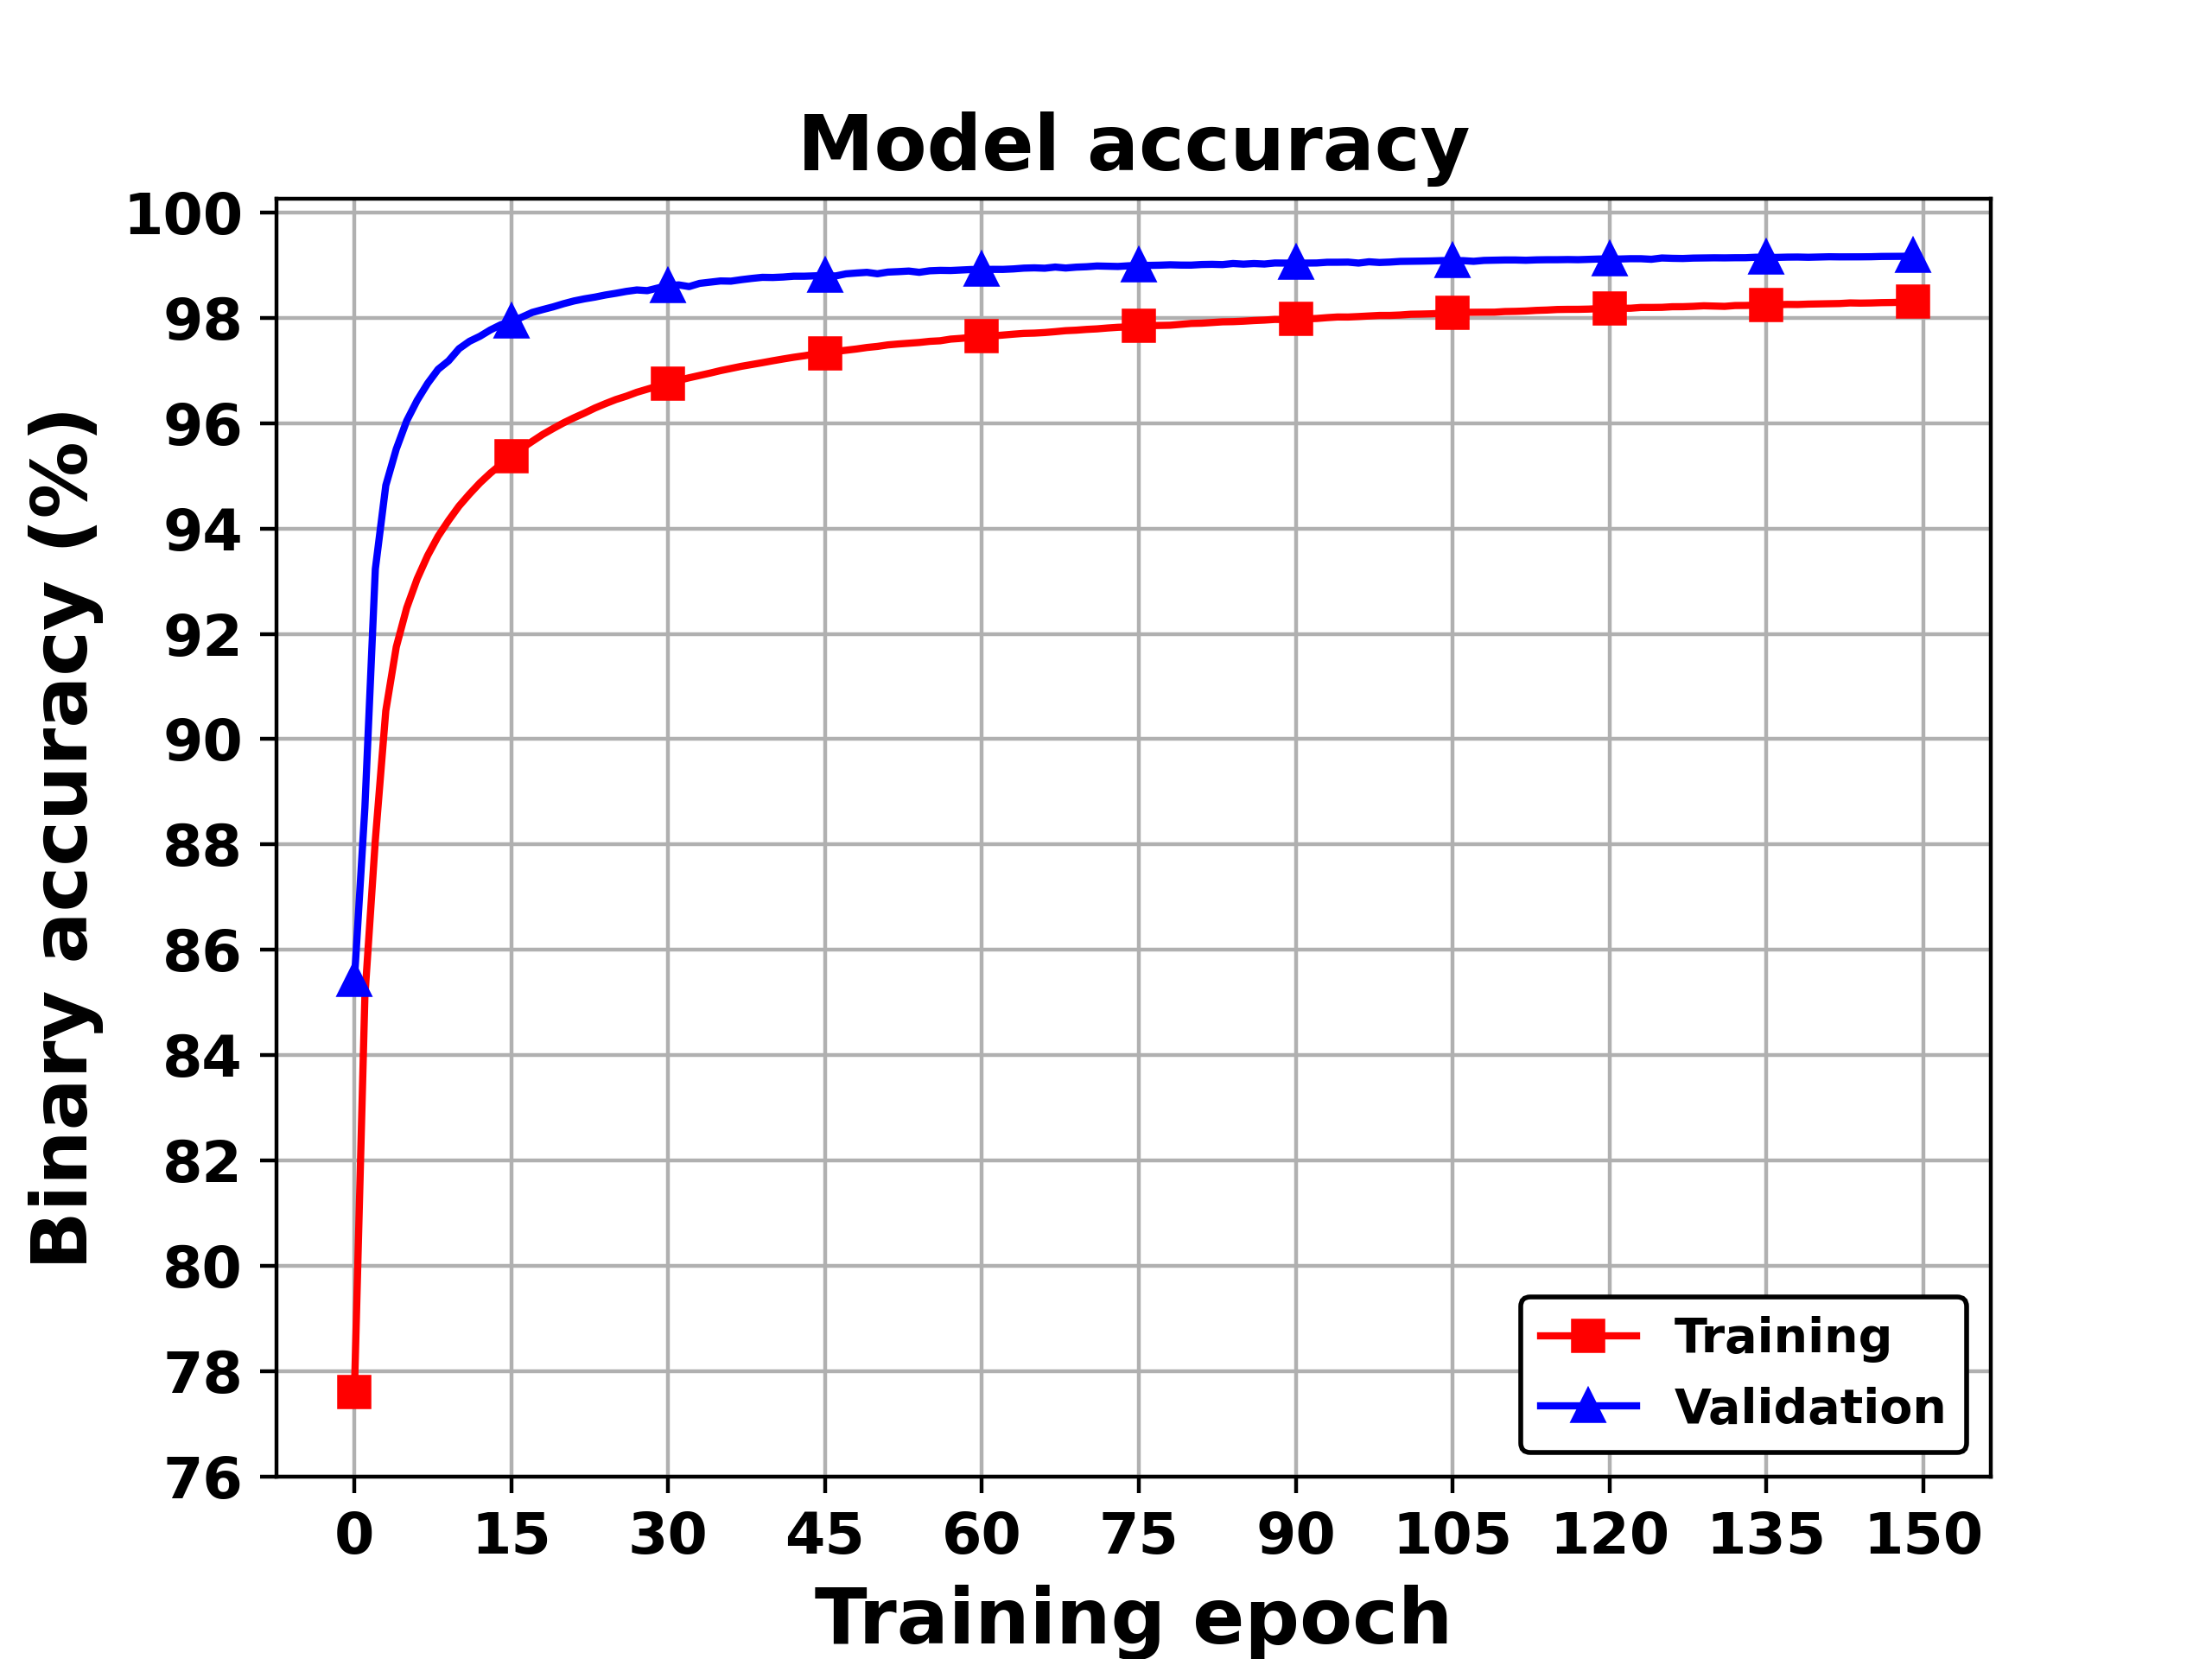
\includegraphics[width=\textwidth]{Figures/Accuracy_FCN_3_512_sim_1638k_fading_SNR_10dB_slots_13_mux_ue_0_1_2_3_4_5_6_7_8_9_10_11_12.png}
         \caption{}
         \label{fig: acc_vs_epoch}
     \end{subfigure}
     \\
     \begin{subfigure}[b]{0.48\textwidth}
         \centering
         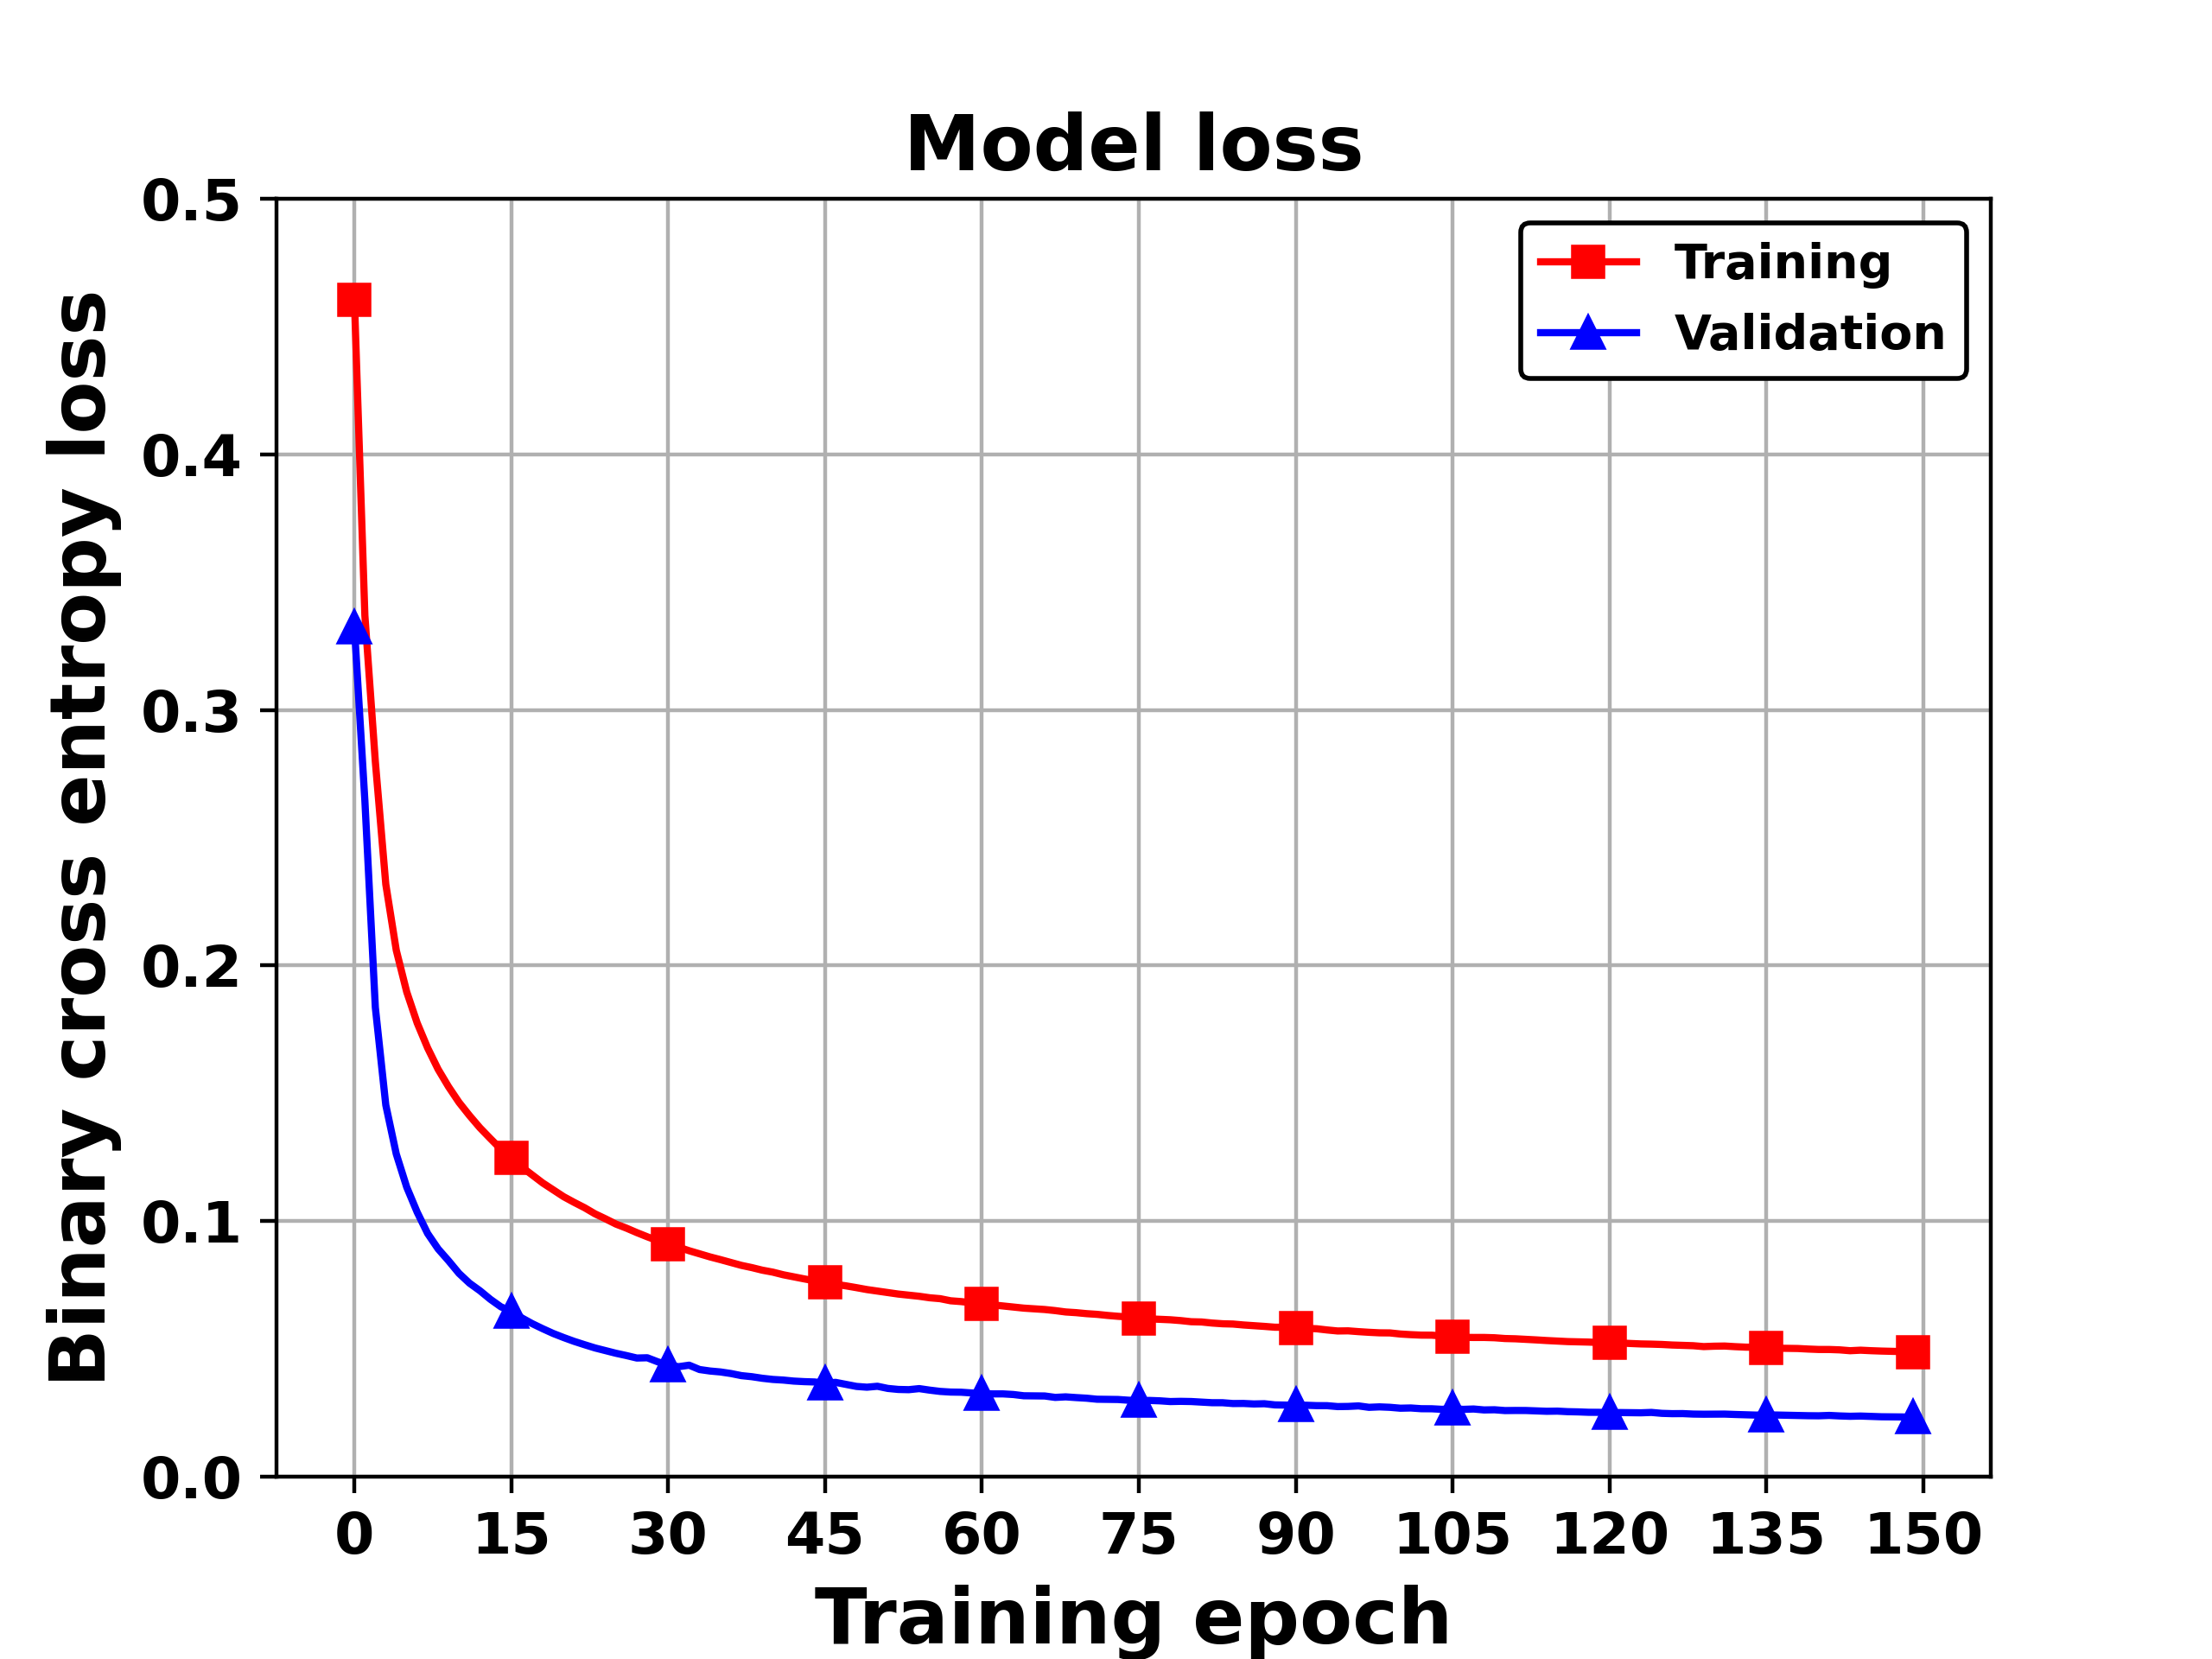
\includegraphics[width=\textwidth]{Figures/Loss_FCN_3_512_sim_1638k_fading_SNR_10dB_slots_13_mux_ue_0_1_2_3_4_5_6_7_8_9_10_11_12.png}
         \caption{}
         \label{fig: loss_vs_epoch}
     \end{subfigure}
        \caption{Training was performed only using simulated data at SNR = $10$ dB. (a) Model Accuracy vs. Epoch for simulated data. (b) Model Loss vs. Epoch for simulated data.}
        \label{fig: acc_loss_vs_epoch}
\end{figure}

Figure~\ref{fig: acc_vs_snr_sim} shows the test accuracy of the model versus SNR for simulated data. Figure~\ref{fig: acc_vs_snr_hw} shows the test accuracy of the model versus SNR for hardware-captured data. In both cases, the test dataset for each SNR contains a combination of all possible values of $N_{UE} = \{0, 1, 2, \dots, 12\}$. Both Figures~\ref{fig: acc_vs_snr_sim} and~\ref{fig: acc_vs_snr_hw} show that model accuracy increases with SNR. For the simulated data, the model significantly outperforms the DFT algorithm for all values of $\Delta$.

For the hardware captured data, when $\Delta = 0$, the model performs slightly better than the DFT algorithm. But as the SNR increases, the accuracies of the model and that of the DFT algorithm converge. This is because $\Delta = 0$ constitutes a best-case scenario in which both algorithms are aided by the fact that the receiver knows exactly how many UEs are multiplexed. At higher values of $\Delta$, the convergence is not seen, and the NN model shows a significant gain compared to the DFT algorithm. 

Furthermore, from Figures~\ref{fig: acc_vs_snr_sim} and~\ref{fig: acc_vs_snr_hw}, we observe an interesting difference between the performance of the neural network with simulated data versus hardware captured data. For all values of $\Delta$, there is a significant SNR gain with the hardware data compared to simulated data. For example, when $\Delta = 0$, the accuracy with hardware captured data reaches 100\% at as low an SNR as $5$ dB. In contrast, the accuracy with simulated data requires more than $15$dB SNR to reach 100\%. This difference could be attributed to the characteristics of the datasets themselves. The simulated dataset includes a strong fading component that impairs the transmitted signal. However, owing to the short propagation distance, such a strong fading component is absent in the current 5G testbed setup that was used to obtain the hardware captures. We note that the captures still incorporate other real-world impairments caused by front-end hardware elements like filters, DACs, ADCs, up/down converters, and amplifiers. In summary, the hardware dataset models impairments due to front-end elements well. It also models over-the-air impairments but does not encapsulate all characteristics of a typical communication link between a gNB and UE that might span hundreds of meters. On the other hand, the simulated data models over-the-air characteristics well but it doesn't model impairments due to hardware elements. We also point out that the IIT Madras 5G Testbed is moving towards deployment of Remote Radio Heads at on-campus sites which will allow the inclusion of even more realistic field data into future work.

Another observation from Figures~\ref{fig: acc_vs_snr_sim} and~\ref{fig: acc_vs_snr_hw} is that the DFT algorithm performs worse on hardware data, showing that it is negatively affected not only by impairments from hardware elements but also by even the slightest over-the-air fading. On the other hand, the NN Model outperforms the DFT method in all scenarios of hardware and simulated datasets.

Figure~\ref{fig: acc_vs_mux_ue_sim} shows the test accuracy of the NN model versus the number of multiplexed UEs ($N_{UE}$) for simulated data. Figure~\ref{fig: acc_vs_mux_ue_hw} shows the test accuracy of the NN model versus the number of multiplexed UEs ($N_{UE}$) for hardware-captured data. In both cases, the test dataset for each $N_{UE}$ contains a combination of all possible values of SNR $= \{0, 5, 10, 15, 20\}$ dB. It is clear that the accuracy decreases as the maximum offset $\Delta$ increases. Note that no value is plotted when $N_{UE} = 0$ and $\Delta=0$ since this case corresponds to the scenario in which no UEs are transmitting on a given Resource Block and the receiver knows apriori that no UEs are scheduled as well. In this case, the receiver need not even run. When $N_{UE} = 12$, all the multiplexed UEs transmit only Scheduling Requests (SR). For both the simulated and hardware datasets, the DFT algorithm selects all 12 values from the 12-point DFT and assigns one value to each UE. Since all UEs are transmitting SRs, the order of assignment doesn't matter, and hence the accuracy is always 100\%. The NN model also seems to recognize that the only scenario in which 12 UEs can be multiplexed is when they all transmit exactly the same information, i.e., SRs. 

Lower values of $N_{UE}$ tend to result in lower accuracy values. This is because the DFT algorithm picks up the top $N_{UE}$ values of the 12-point DFT, and the probability of a true value lying in one of the $12-N_{UE}$ locations increases as $N_{UE}$ decreases. We observe a similar pattern in the case of decoding with the proposed UCINet0 as well.

\begin{figure}[ht!]
    \captionsetup{justification=justified}
     \centering
     \begin{subfigure}[b]{0.48\textwidth}
         \centering
         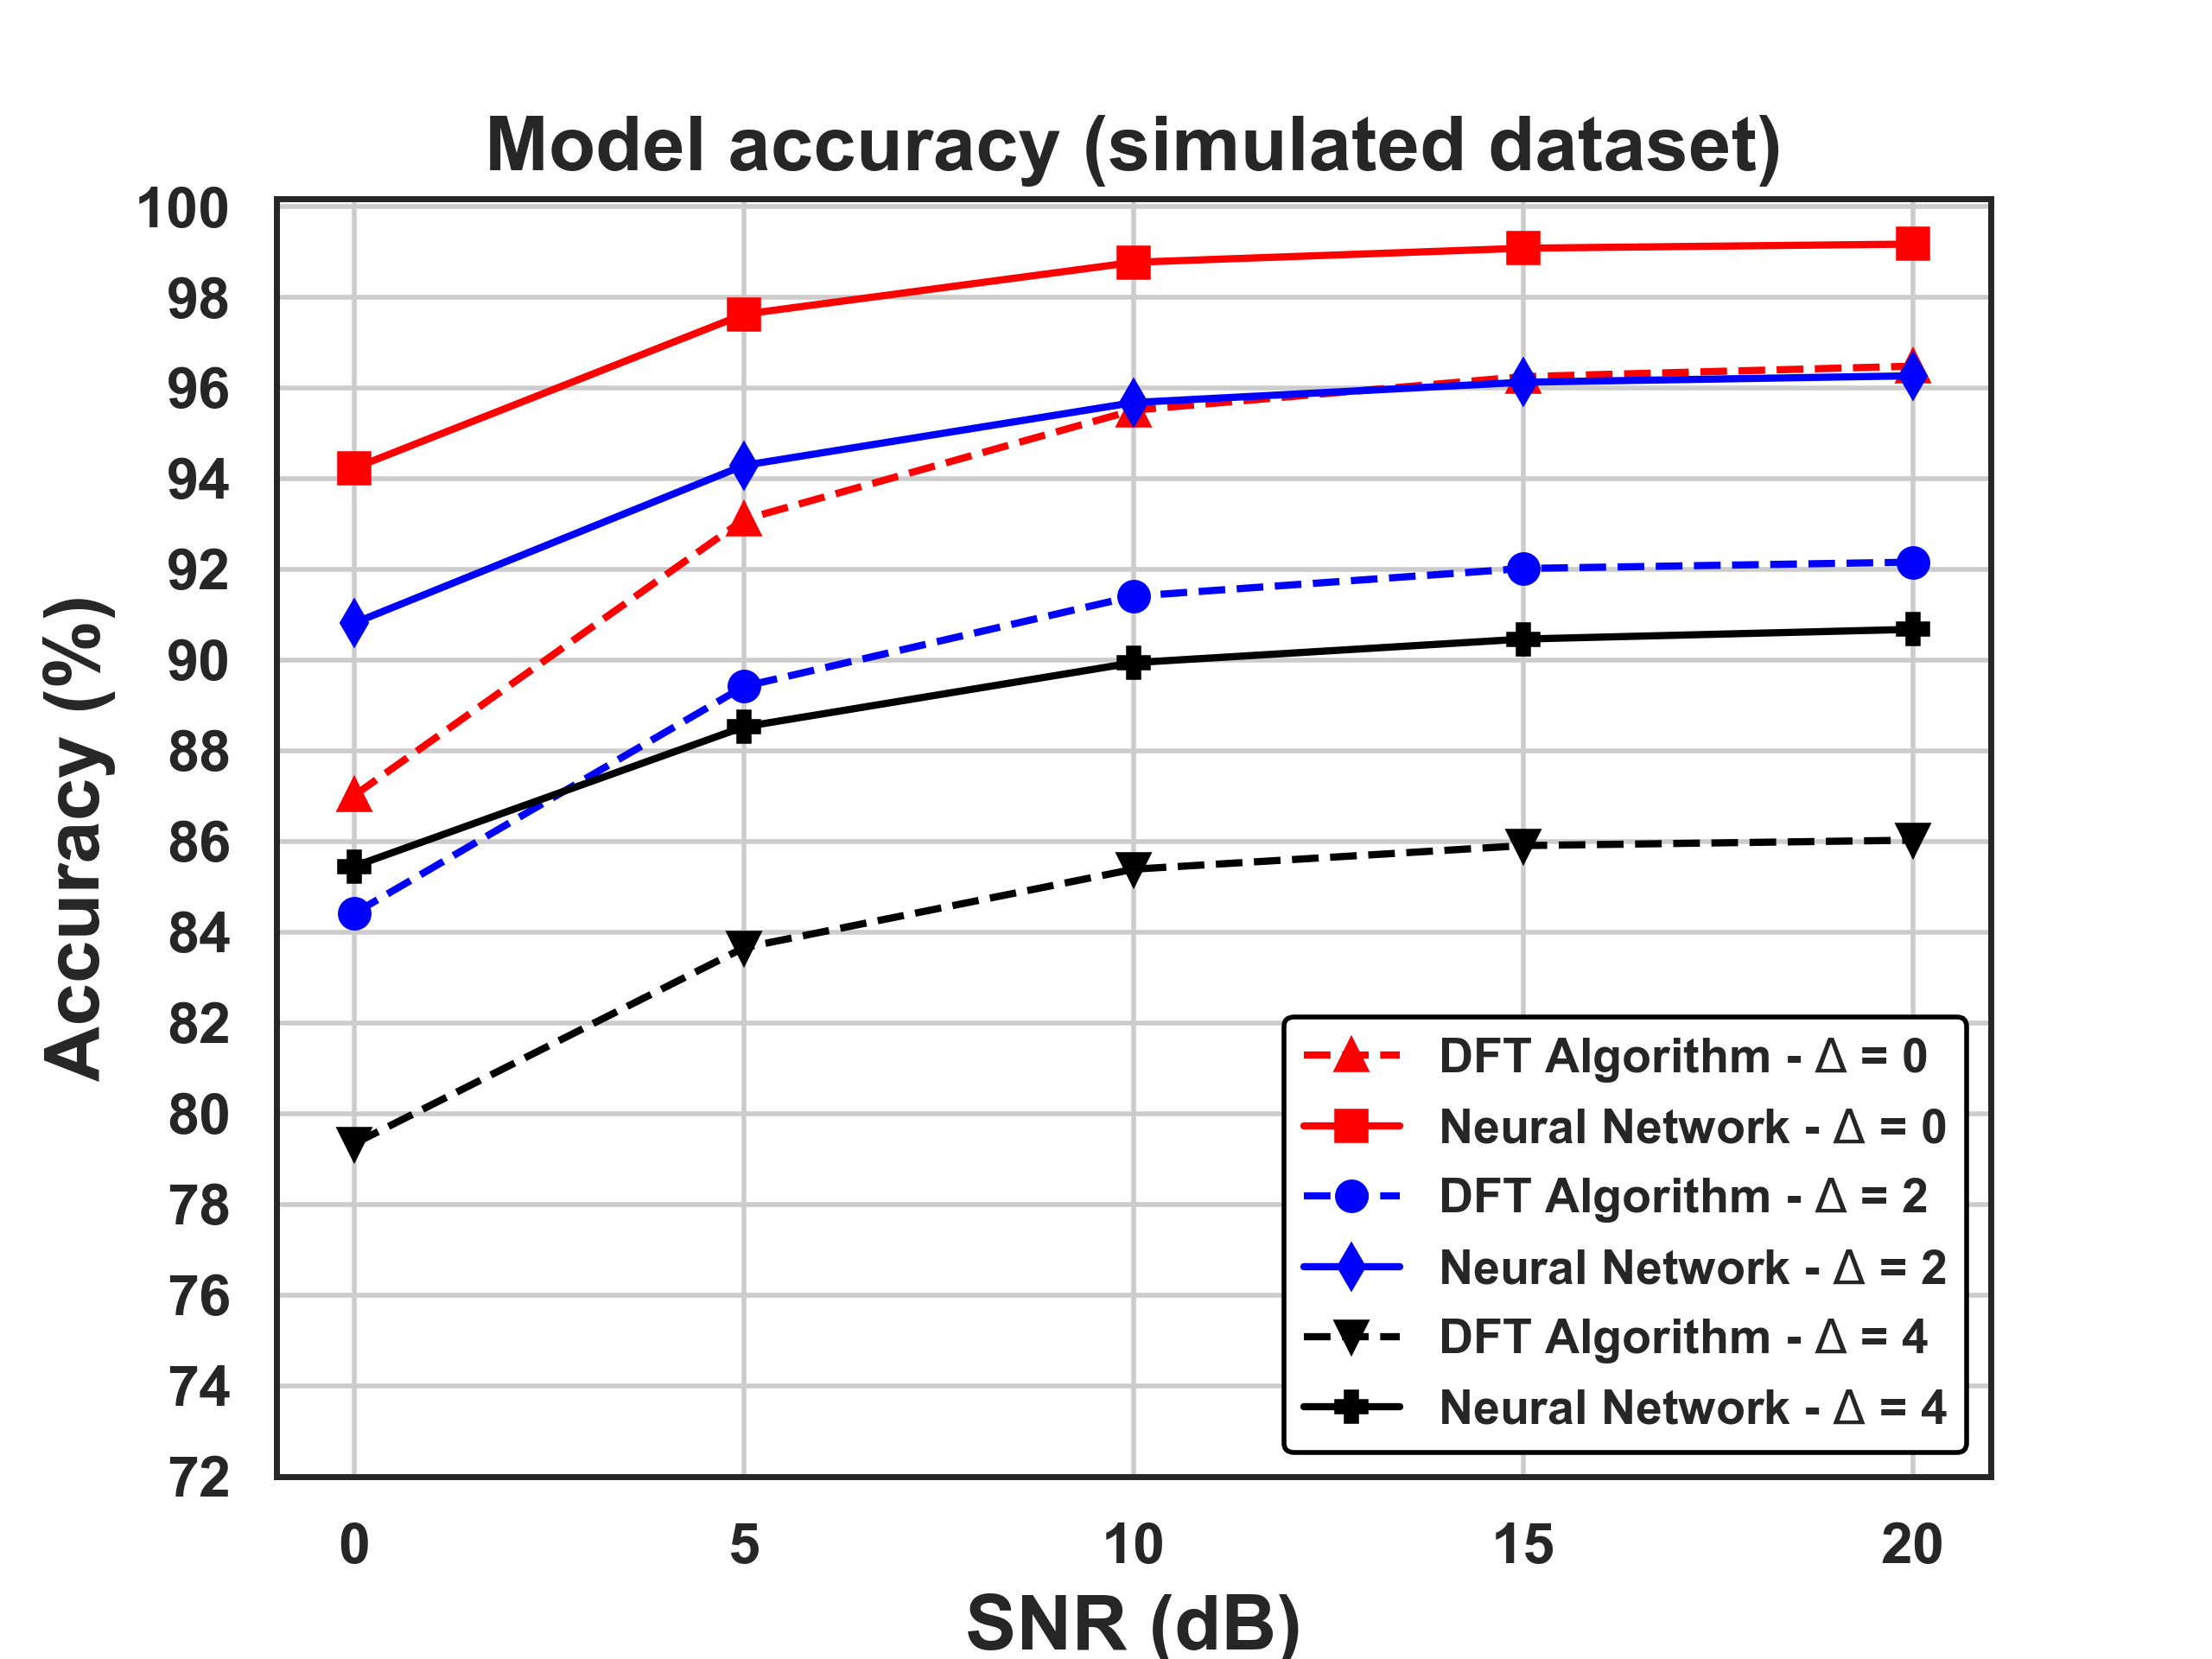
\includegraphics[width=\textwidth]{Figures/Acc_vs_SNR_FCN_3_512_1638k_train_sim_test_sim_in_sz_25_3_layers_512_512_512_nns_out_sz_12_fading_SNR_10dB_slots_13_mux_ue_0__12_epochs_150.png}
         \caption{}
         \label{fig: acc_vs_snr_sim}
     \end{subfigure}
     \\
     \begin{subfigure}[b]{0.48\textwidth}
         \centering
         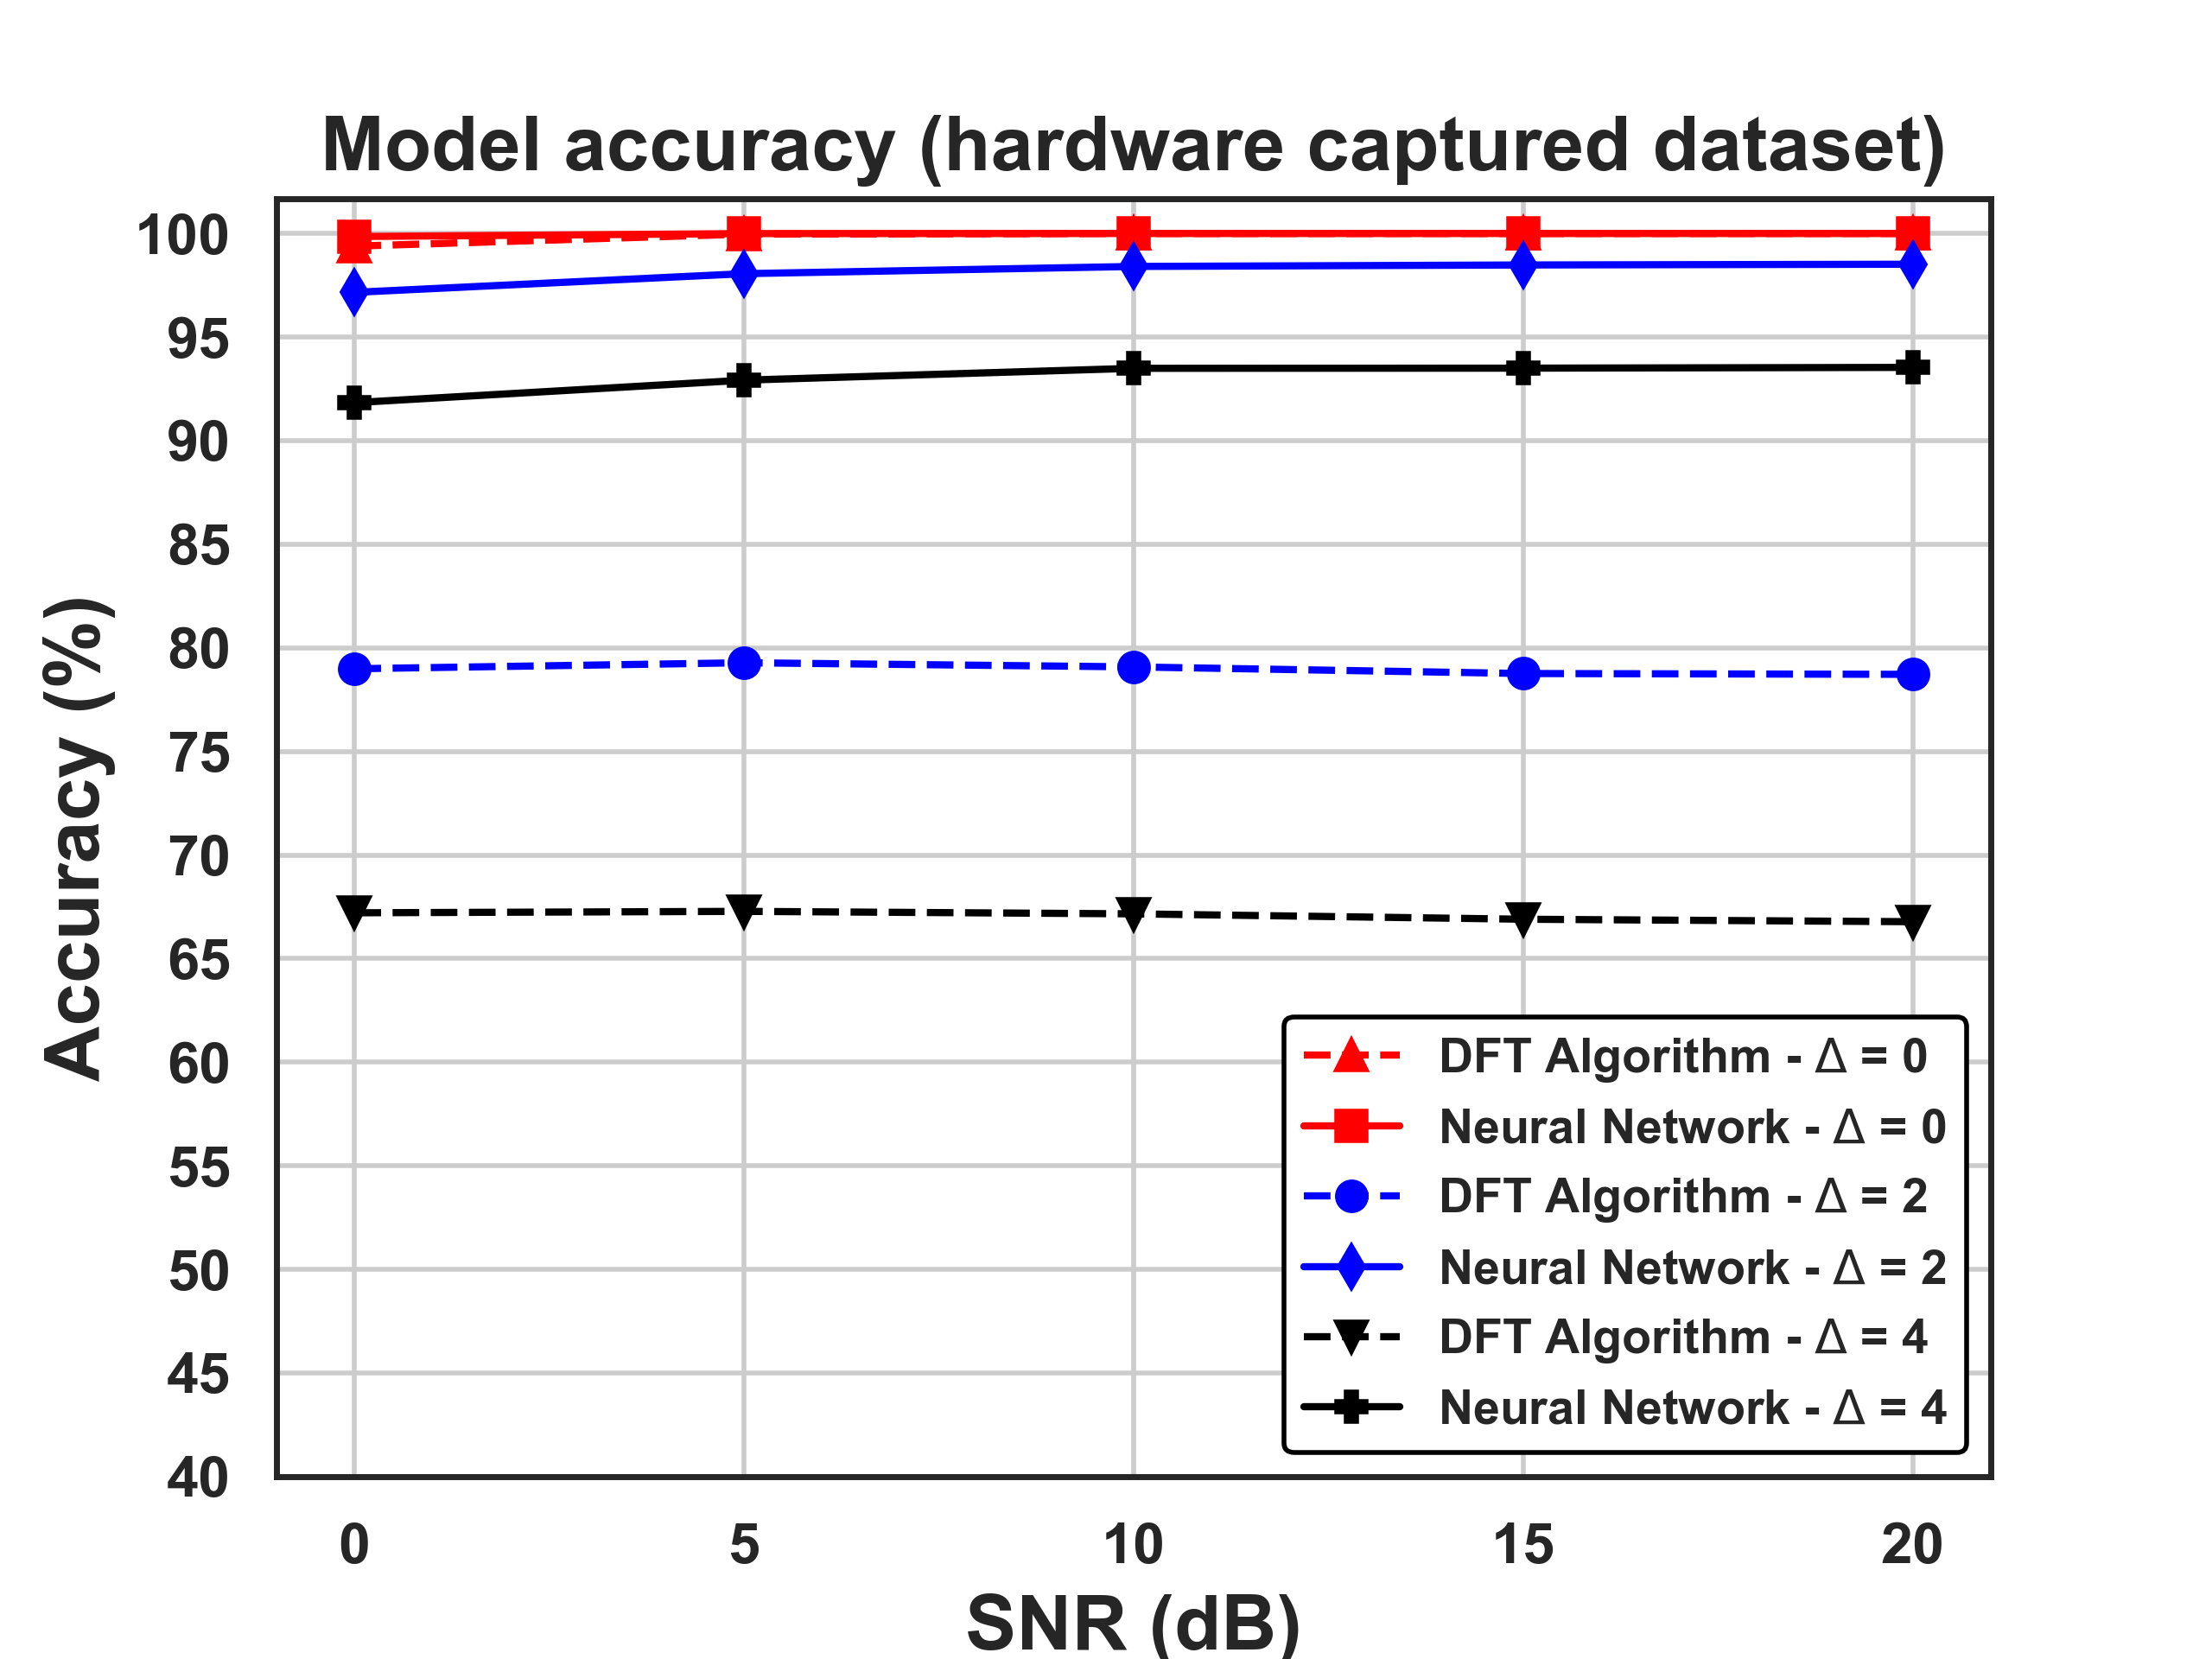
\includegraphics[width=\textwidth]{Figures/Acc_vs_SNR_FCN_3_512_1638k_train_sim_test_hw_in_sz_25_3_layers_512_512_512_nns_out_sz_12_fading_SNR_10dB_slots_13_mux_ue_0__12_epochs_150.png}
         \caption{}
         \label{fig: acc_vs_snr_hw}
     \end{subfigure}
        \caption{Testing Accuracy vs SNR for (a) simulated data and (b) hardware captured data. The test dataset for each SNR contains a combination of $N_{UE} = \{0, 1, 2, \dots, 12\}$.}
        \label{fig: acc_vs_snr}
\end{figure}

\begin{figure}[ht!]
    \captionsetup{justification=justified}
     \centering
     \begin{subfigure}[b]{0.48\textwidth}
         \centering
         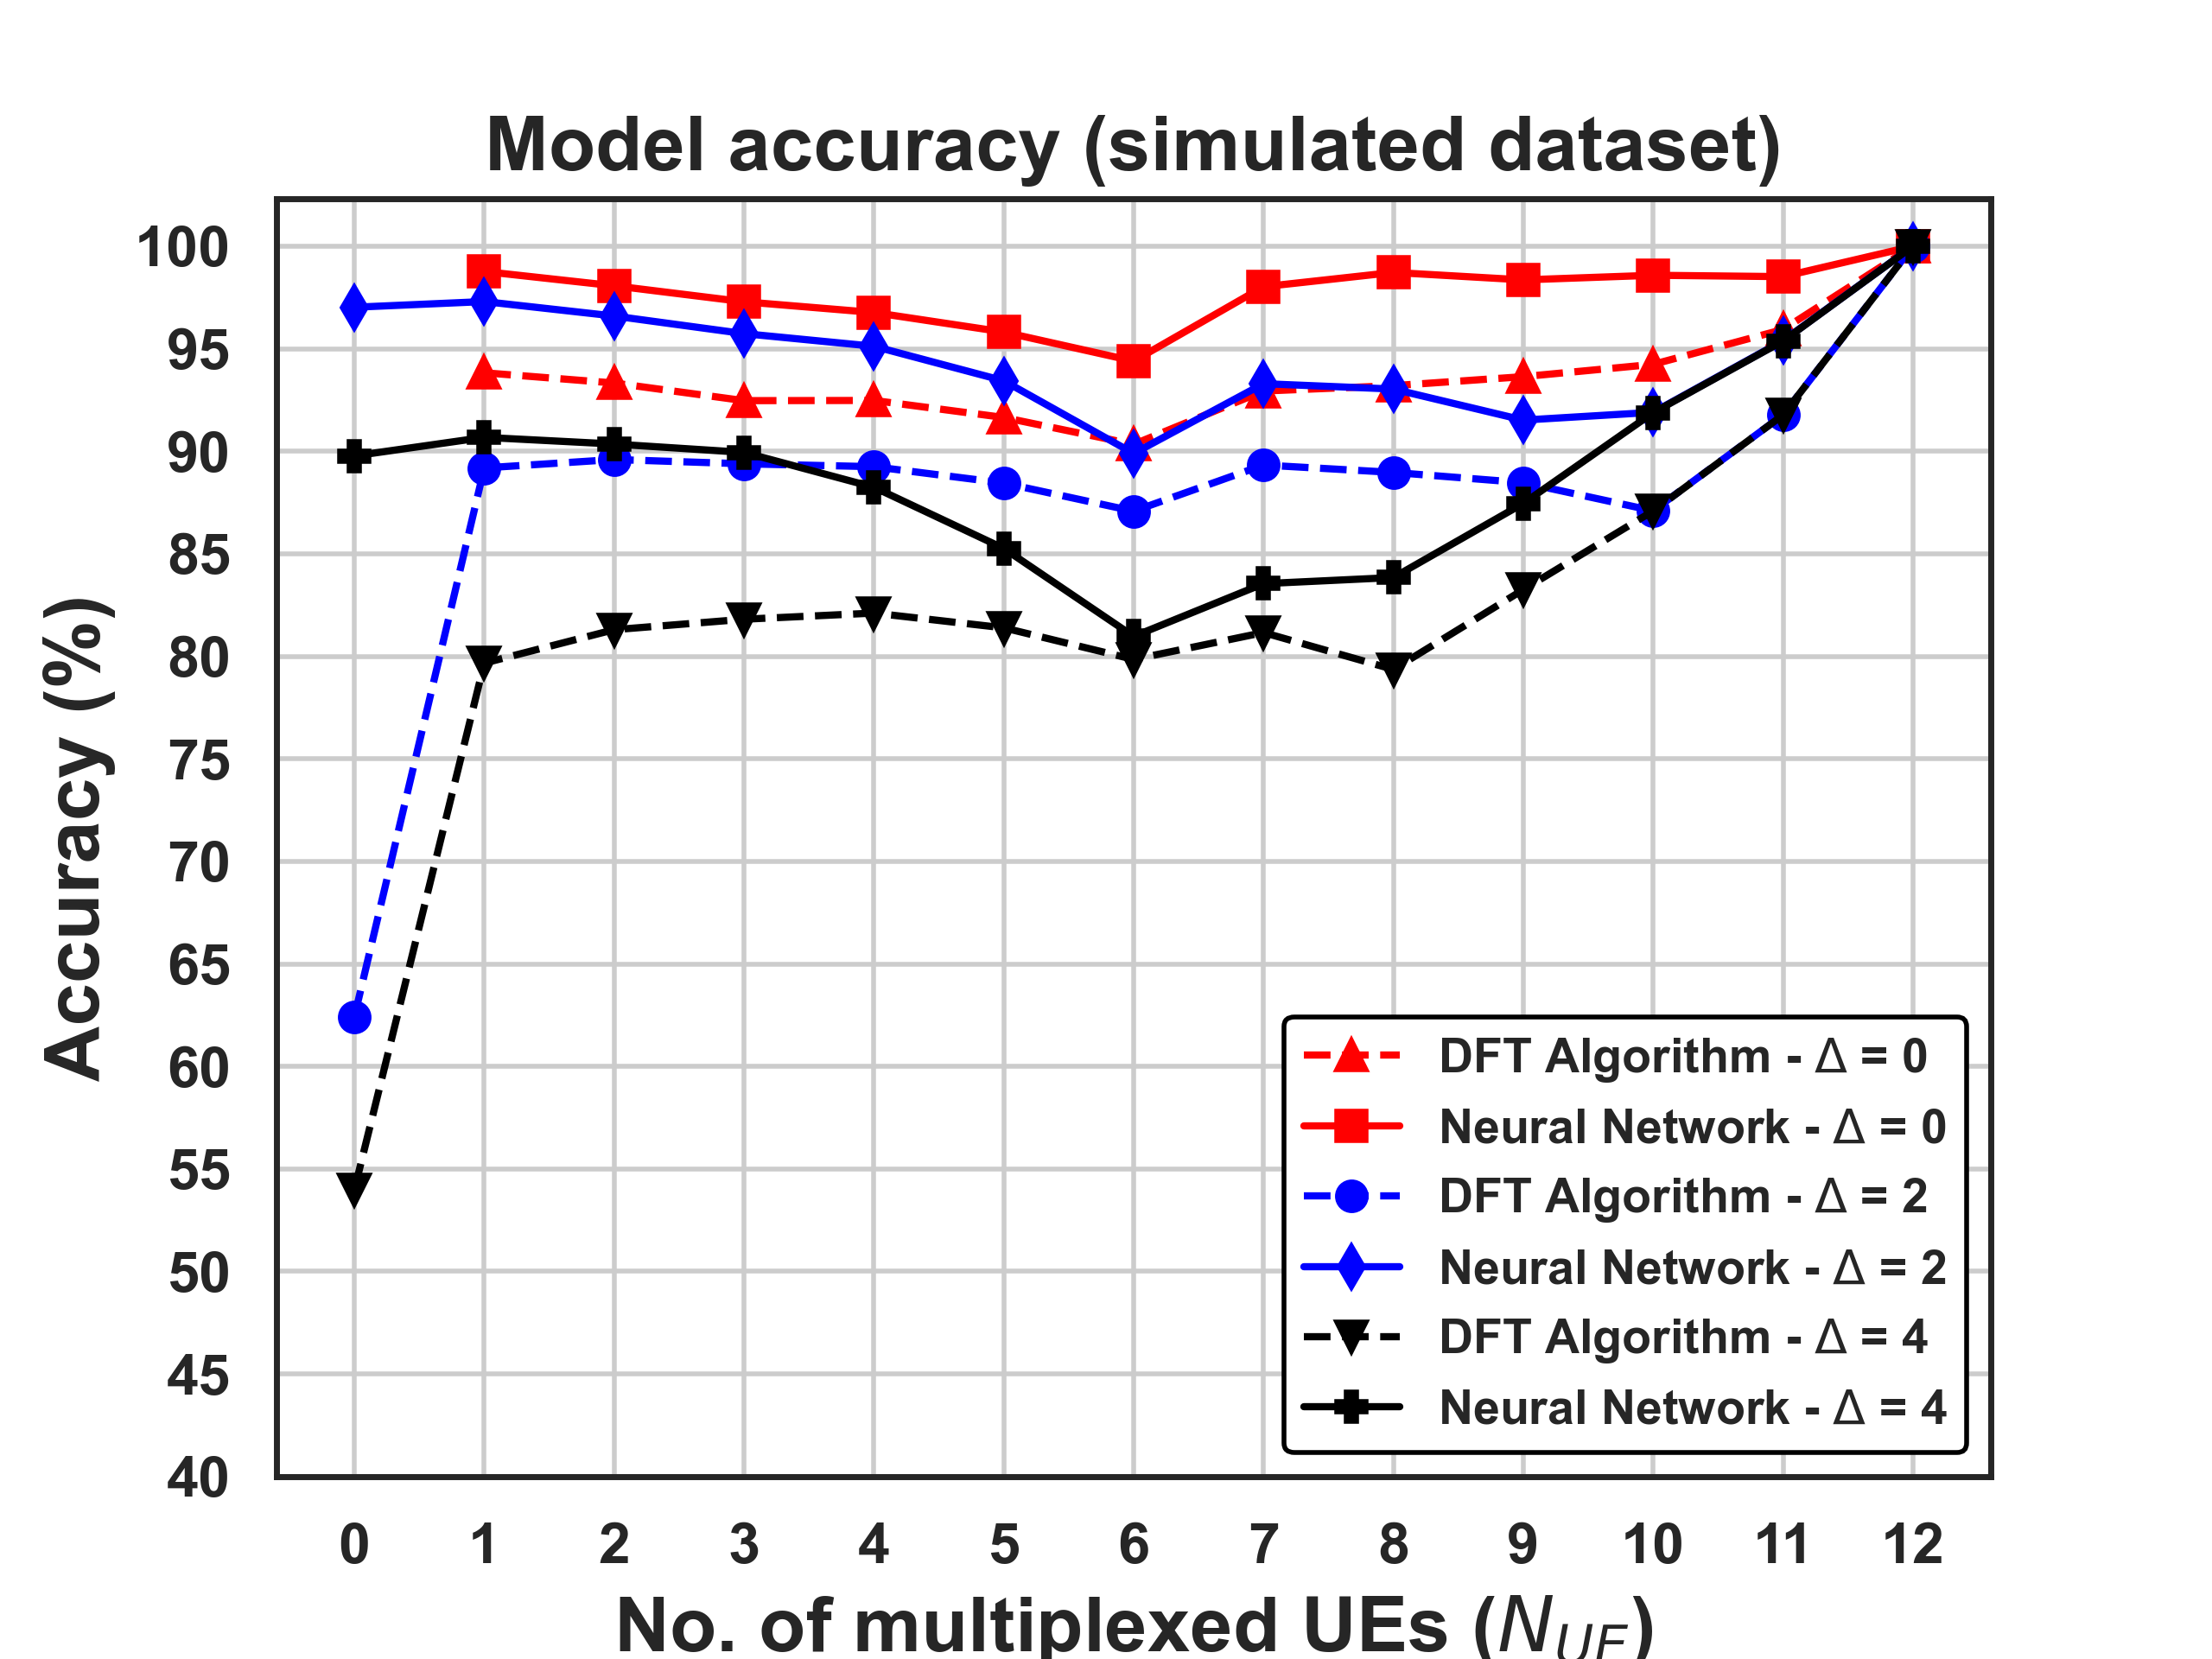
\includegraphics[width=\textwidth]{Figures/Acc_vs_UE_FCN_3_512_1638k_train_sim_test_sim_in_sz_25_3_layers_512_512_512_nns_out_sz_12_fading_SNR_10dB_slots_13_mux_ue_0__12_epochs_150.png}
         \caption{}
         \label{fig: acc_vs_mux_ue_sim}
     \end{subfigure}
     \\
     \begin{subfigure}[b]{0.48\textwidth}
         \centering
         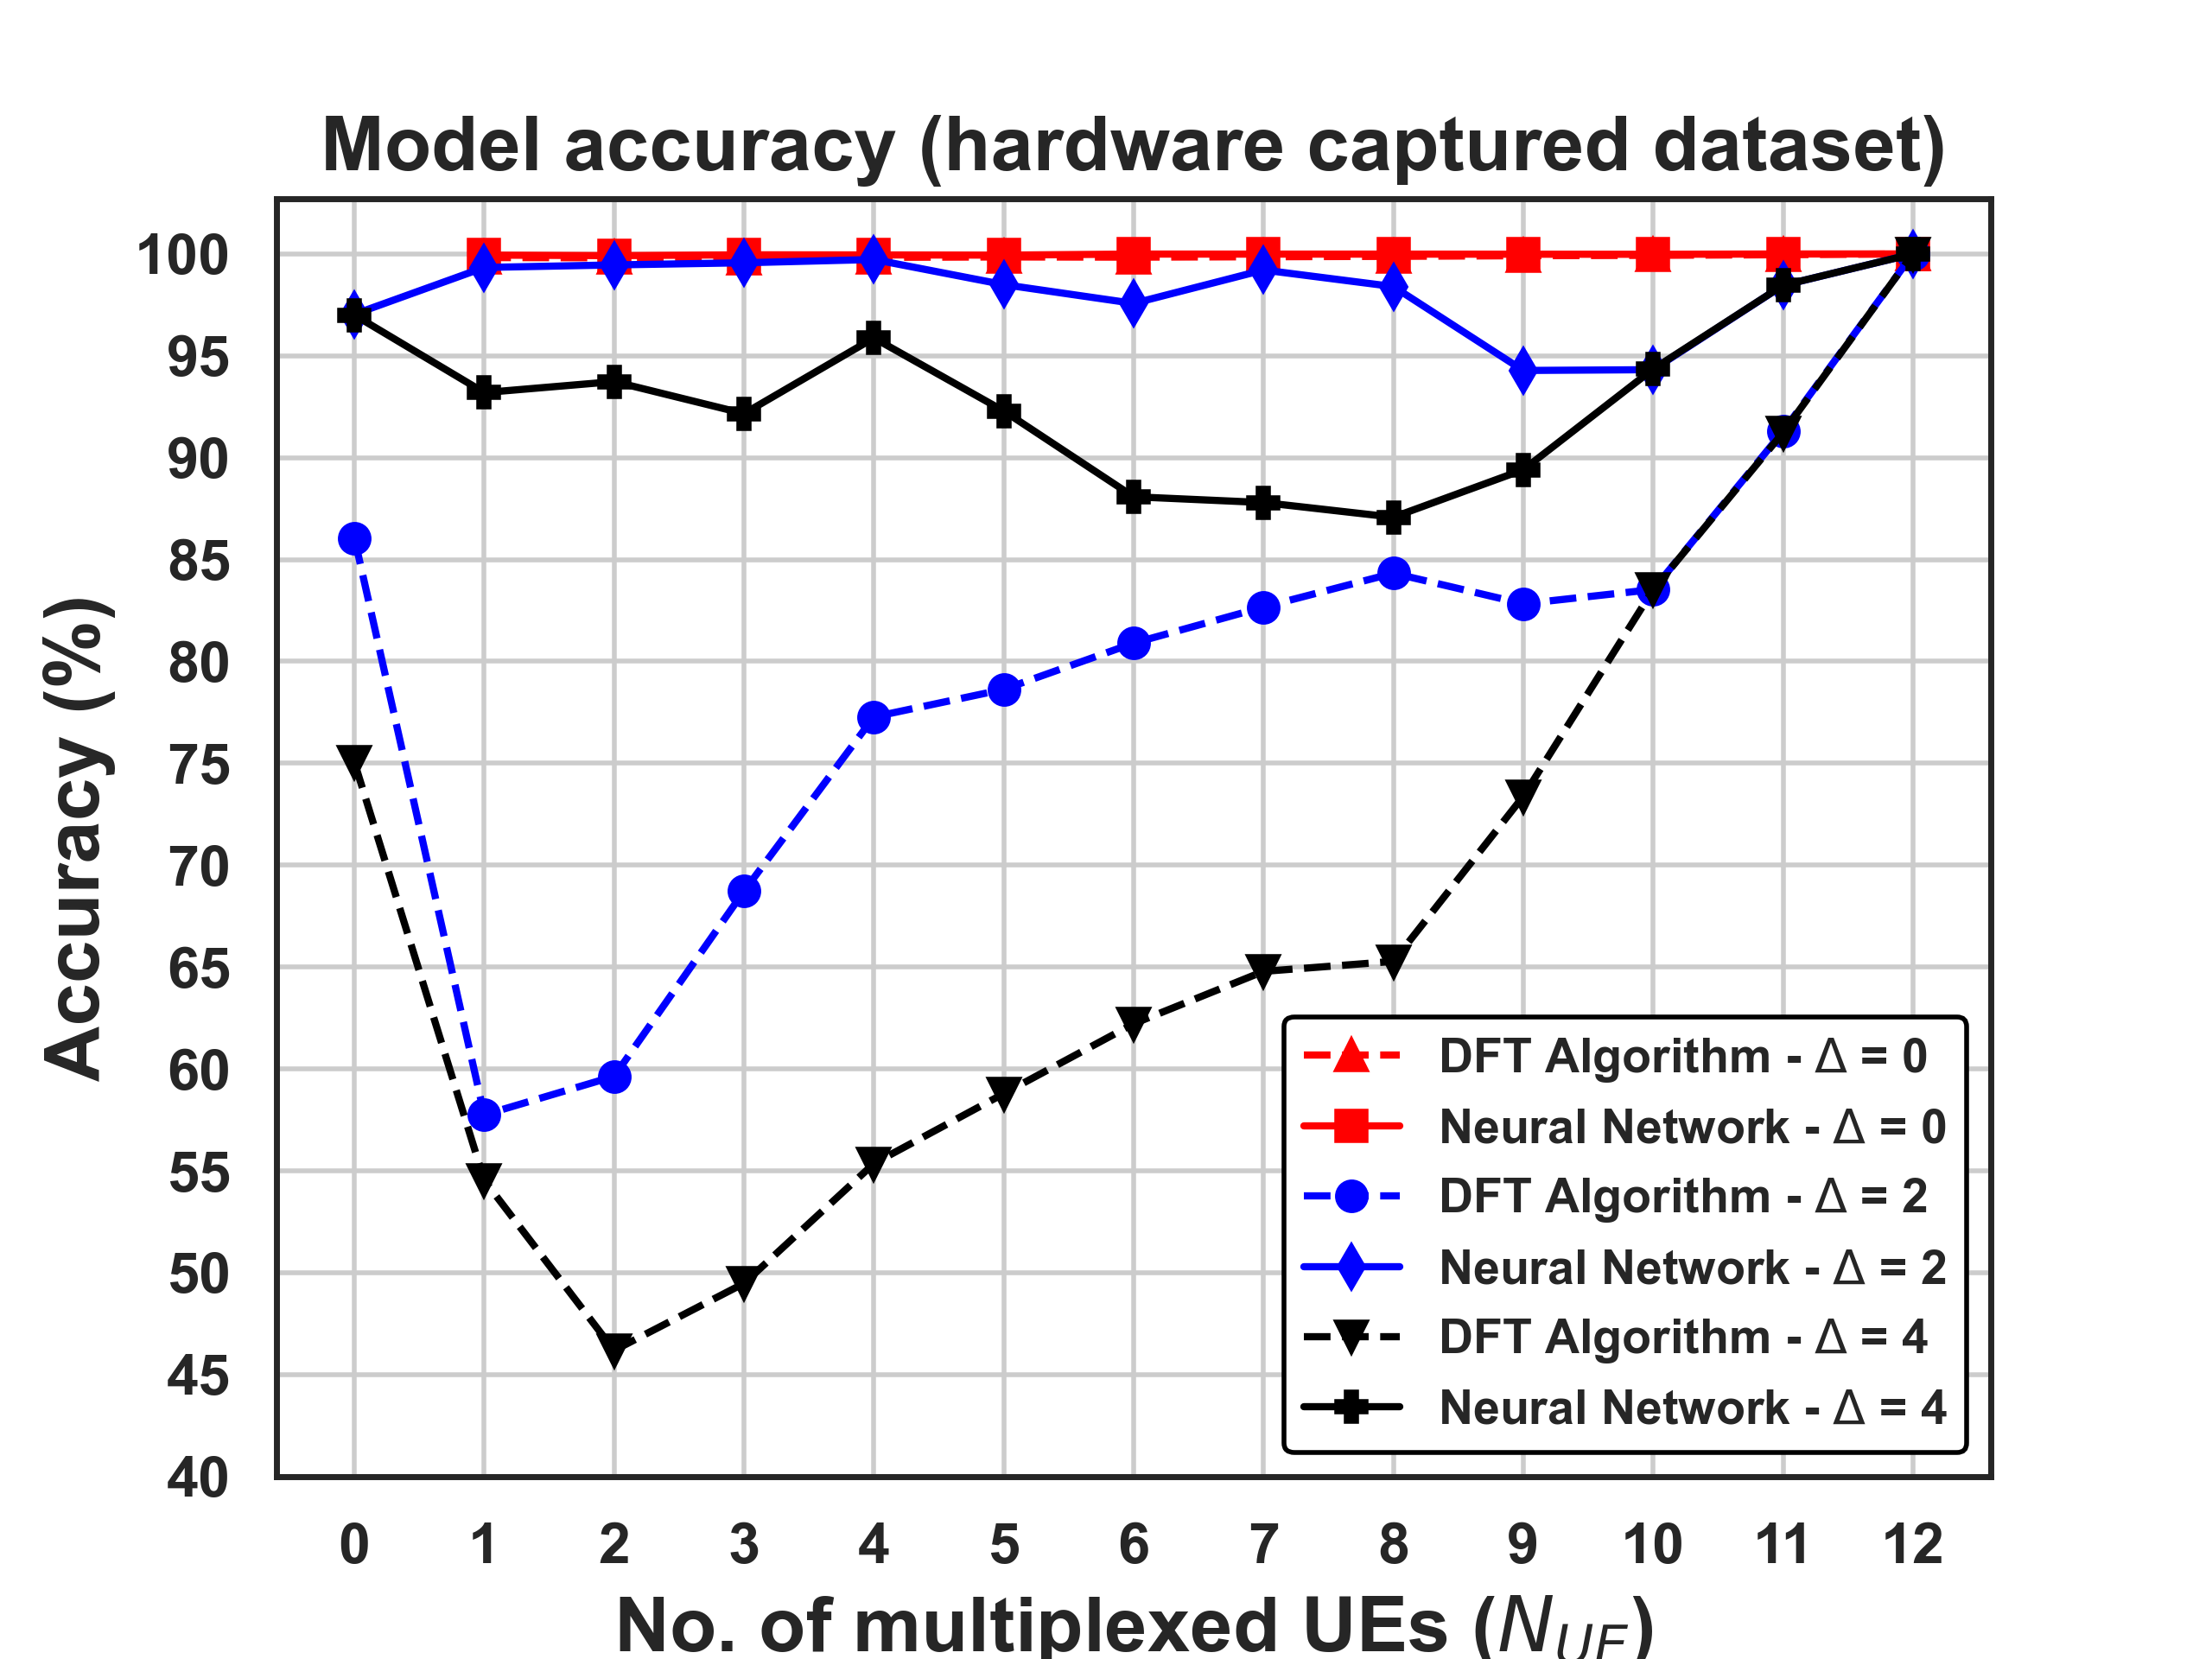
\includegraphics[width=\textwidth]{Figures/Acc_vs_UE_FCN_3_512_1638k_train_sim_test_hw_in_sz_25_3_layers_512_512_512_nns_out_sz_12_fading_SNR_10dB_slots_13_mux_ue_0__12_epochs_150.png}
         \caption{}
         \label{fig: acc_vs_mux_ue_hw}
     \end{subfigure}
        \caption{Testing Accuracy vs Number of Multiplexed UEs ($N_{UE}$) for (a) simulated data and (b) hardware captured data. The test dataset for each value of $N_{UE}$ contains a combination of SNR = $\{0, 5, 10, 15, 20\}$ dB.}
        \label{fig: acc_vs_mux_ue}
\end{figure}


\subsection{Confusion Matrices and Column Charts}
The confusion matrices in Figures~\ref{fig: cm_multilabel_snr_20_off_0} and~\ref{fig: cm_multilabel_snr_20_off_4} indicate the overall multi-label classification performance of the model. Figures~\ref{fig: cm_multilabel_snr_20_off_0} and~\ref{fig: cm_multilabel_snr_20_off_4} show the multi-label confusion matrix for the best ($\Delta = 0$) and worst ($\Delta = 4$) cases of $20$dB SNR respectively, for both simulated data and hardware-captured data. Multi-label classification can be thought of as a combination of several independent binary classifiers. Diagonally dominant confusion matrices indicate that each of the binary classifiers is well-trained. For a given SNR, as $\Delta$ increases, the model leans more towards false positives because the model (whose 25th input is $\Tilde{N}_{UE} \in [N_{UE}, N_{UE} + \Delta]$) is trying to predict $\Tilde{N}_{UE}$ number of UEs. The value of $\Delta$ is always positive, meaning that the number of expected UEs, as indicated by L2, is always greater than or equal to the actual number of UEs transmitting on a given resource allocation. Hence, the model almost always over-predicts. 
\begin{figure}[ht!]
    \captionsetup{justification=justified}
     \centering
     \begin{subfigure}[b]{0.48\textwidth}
         \centering
         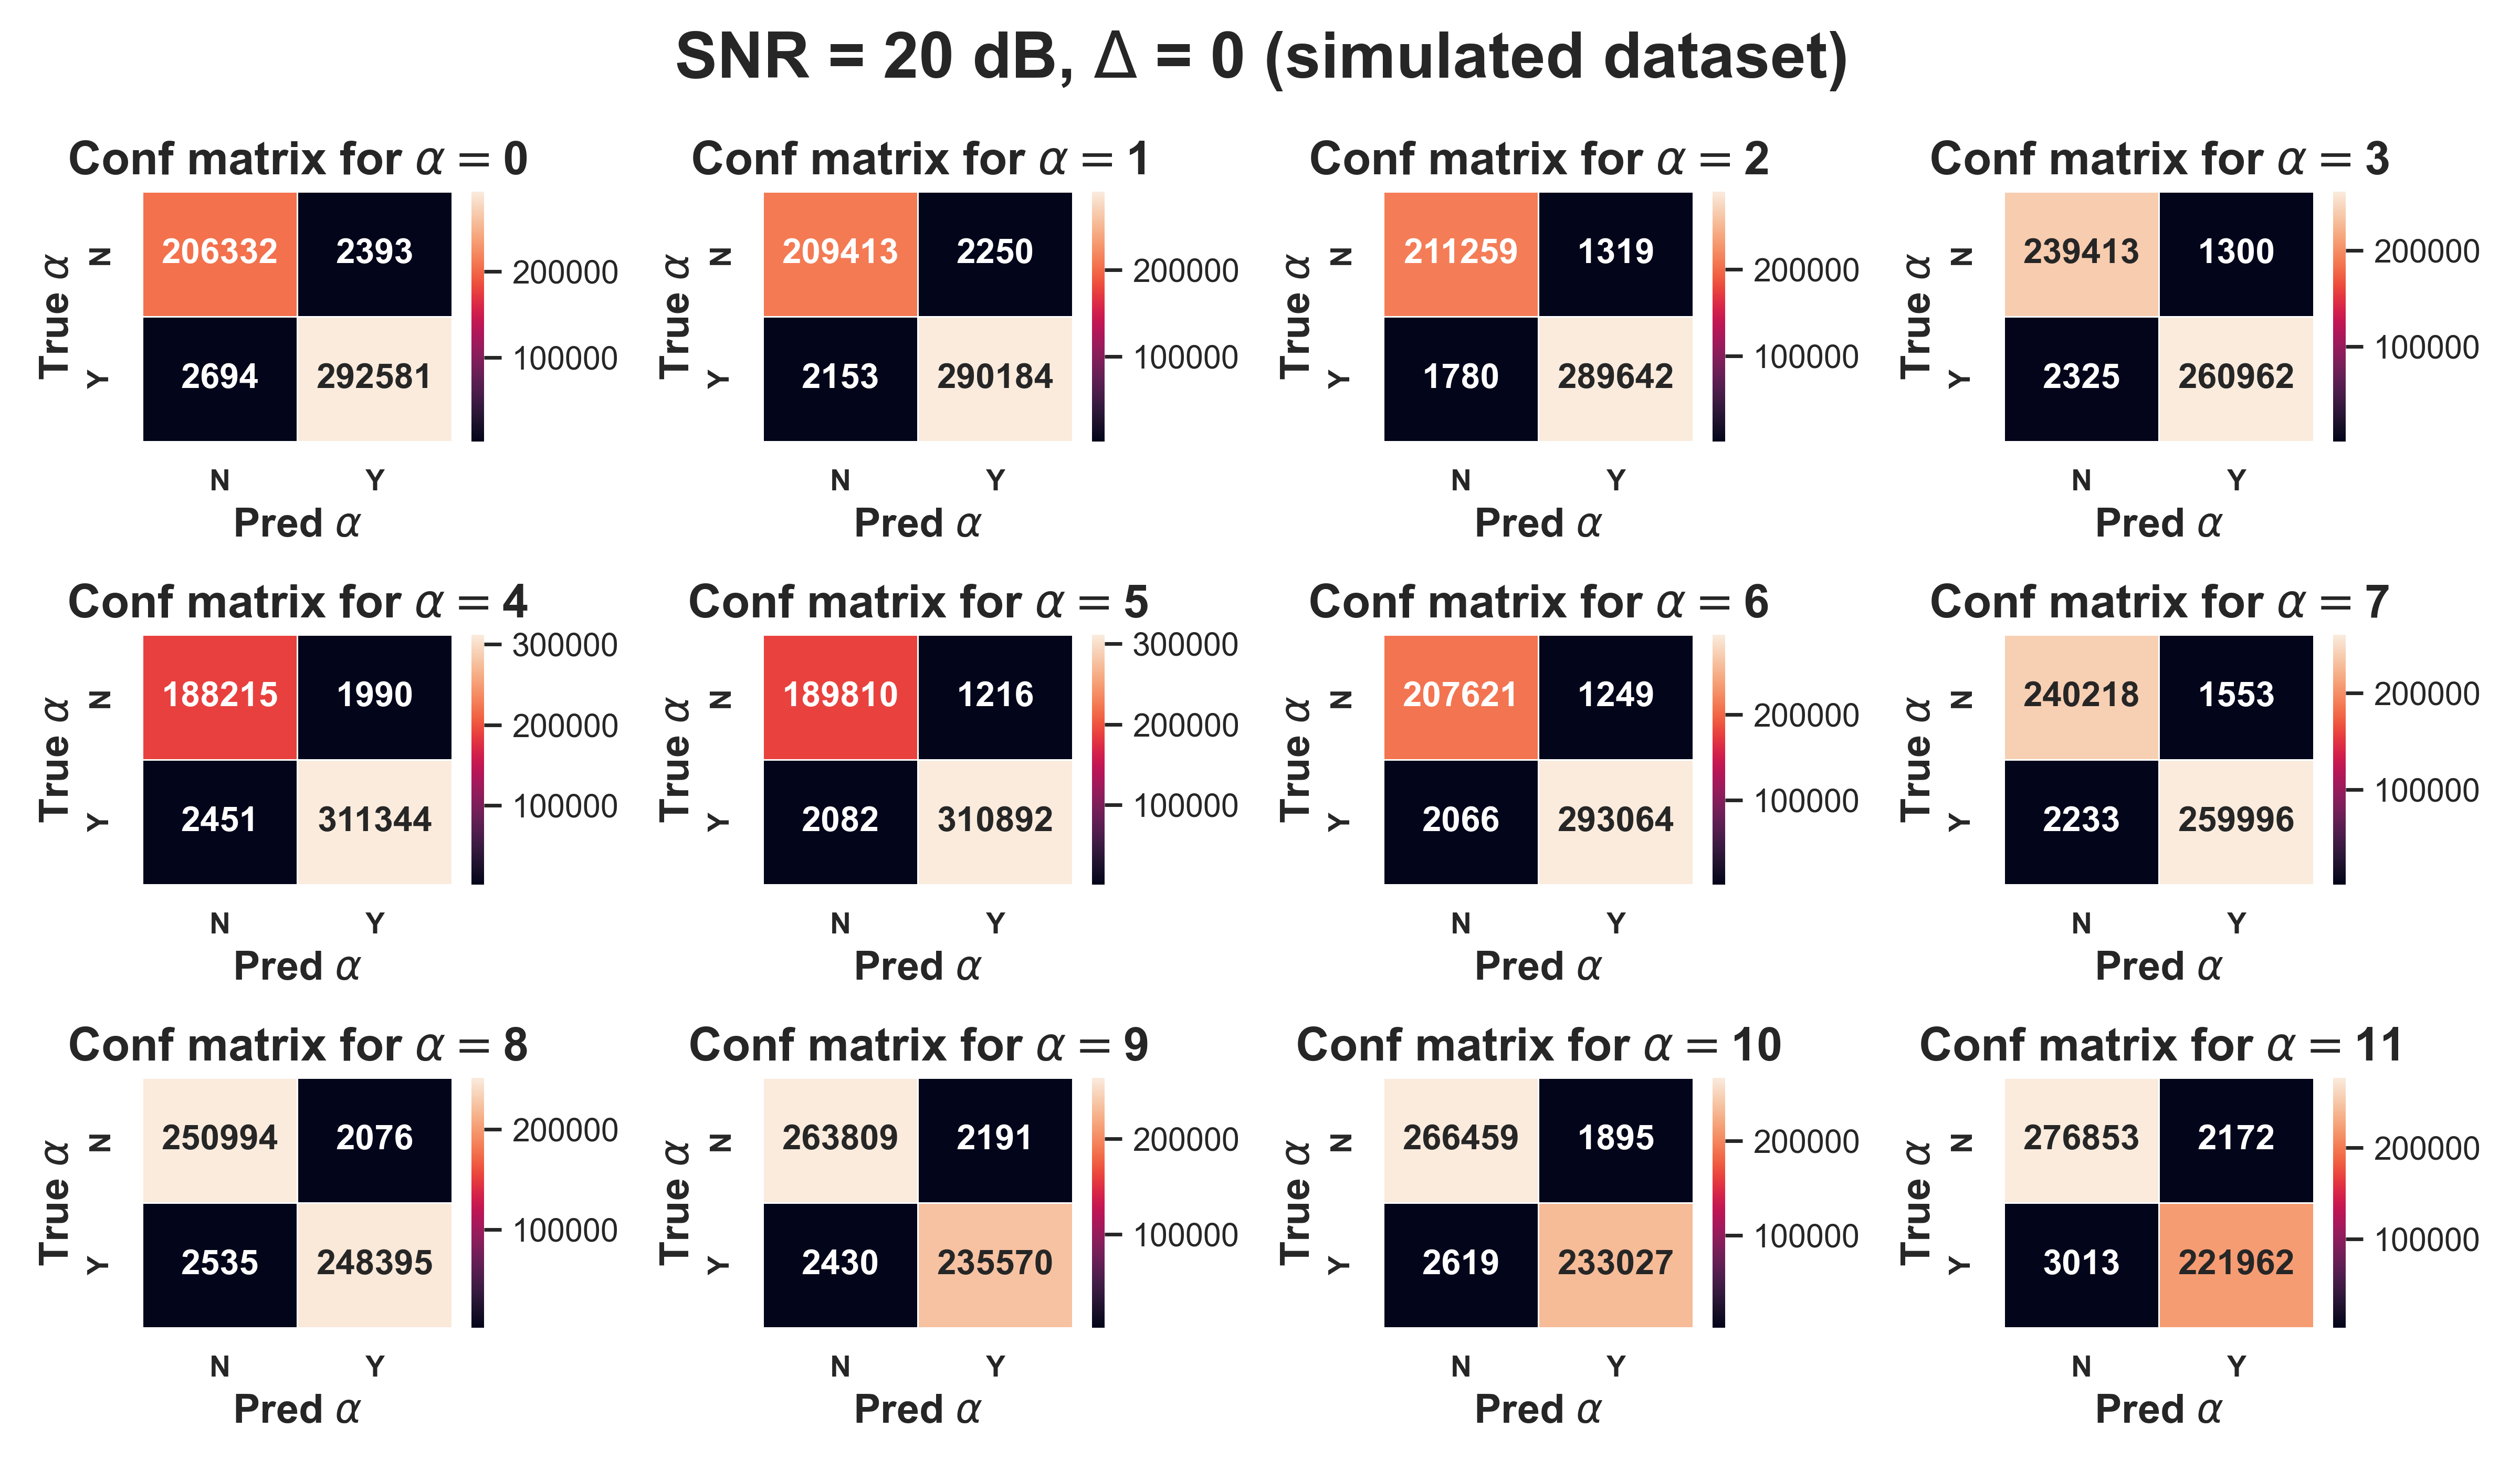
\includegraphics[width=\textwidth]{Figures/Conf_mtx_multi_label_SNR_20_dB_Max_off_0_train_sim_test_sim.png}
         \caption{}
         \label{fig: cm_multilabel_snr_20_off_0_sim}
     \end{subfigure}
     \\
     \begin{subfigure}[b]{0.48\textwidth}
         \centering
         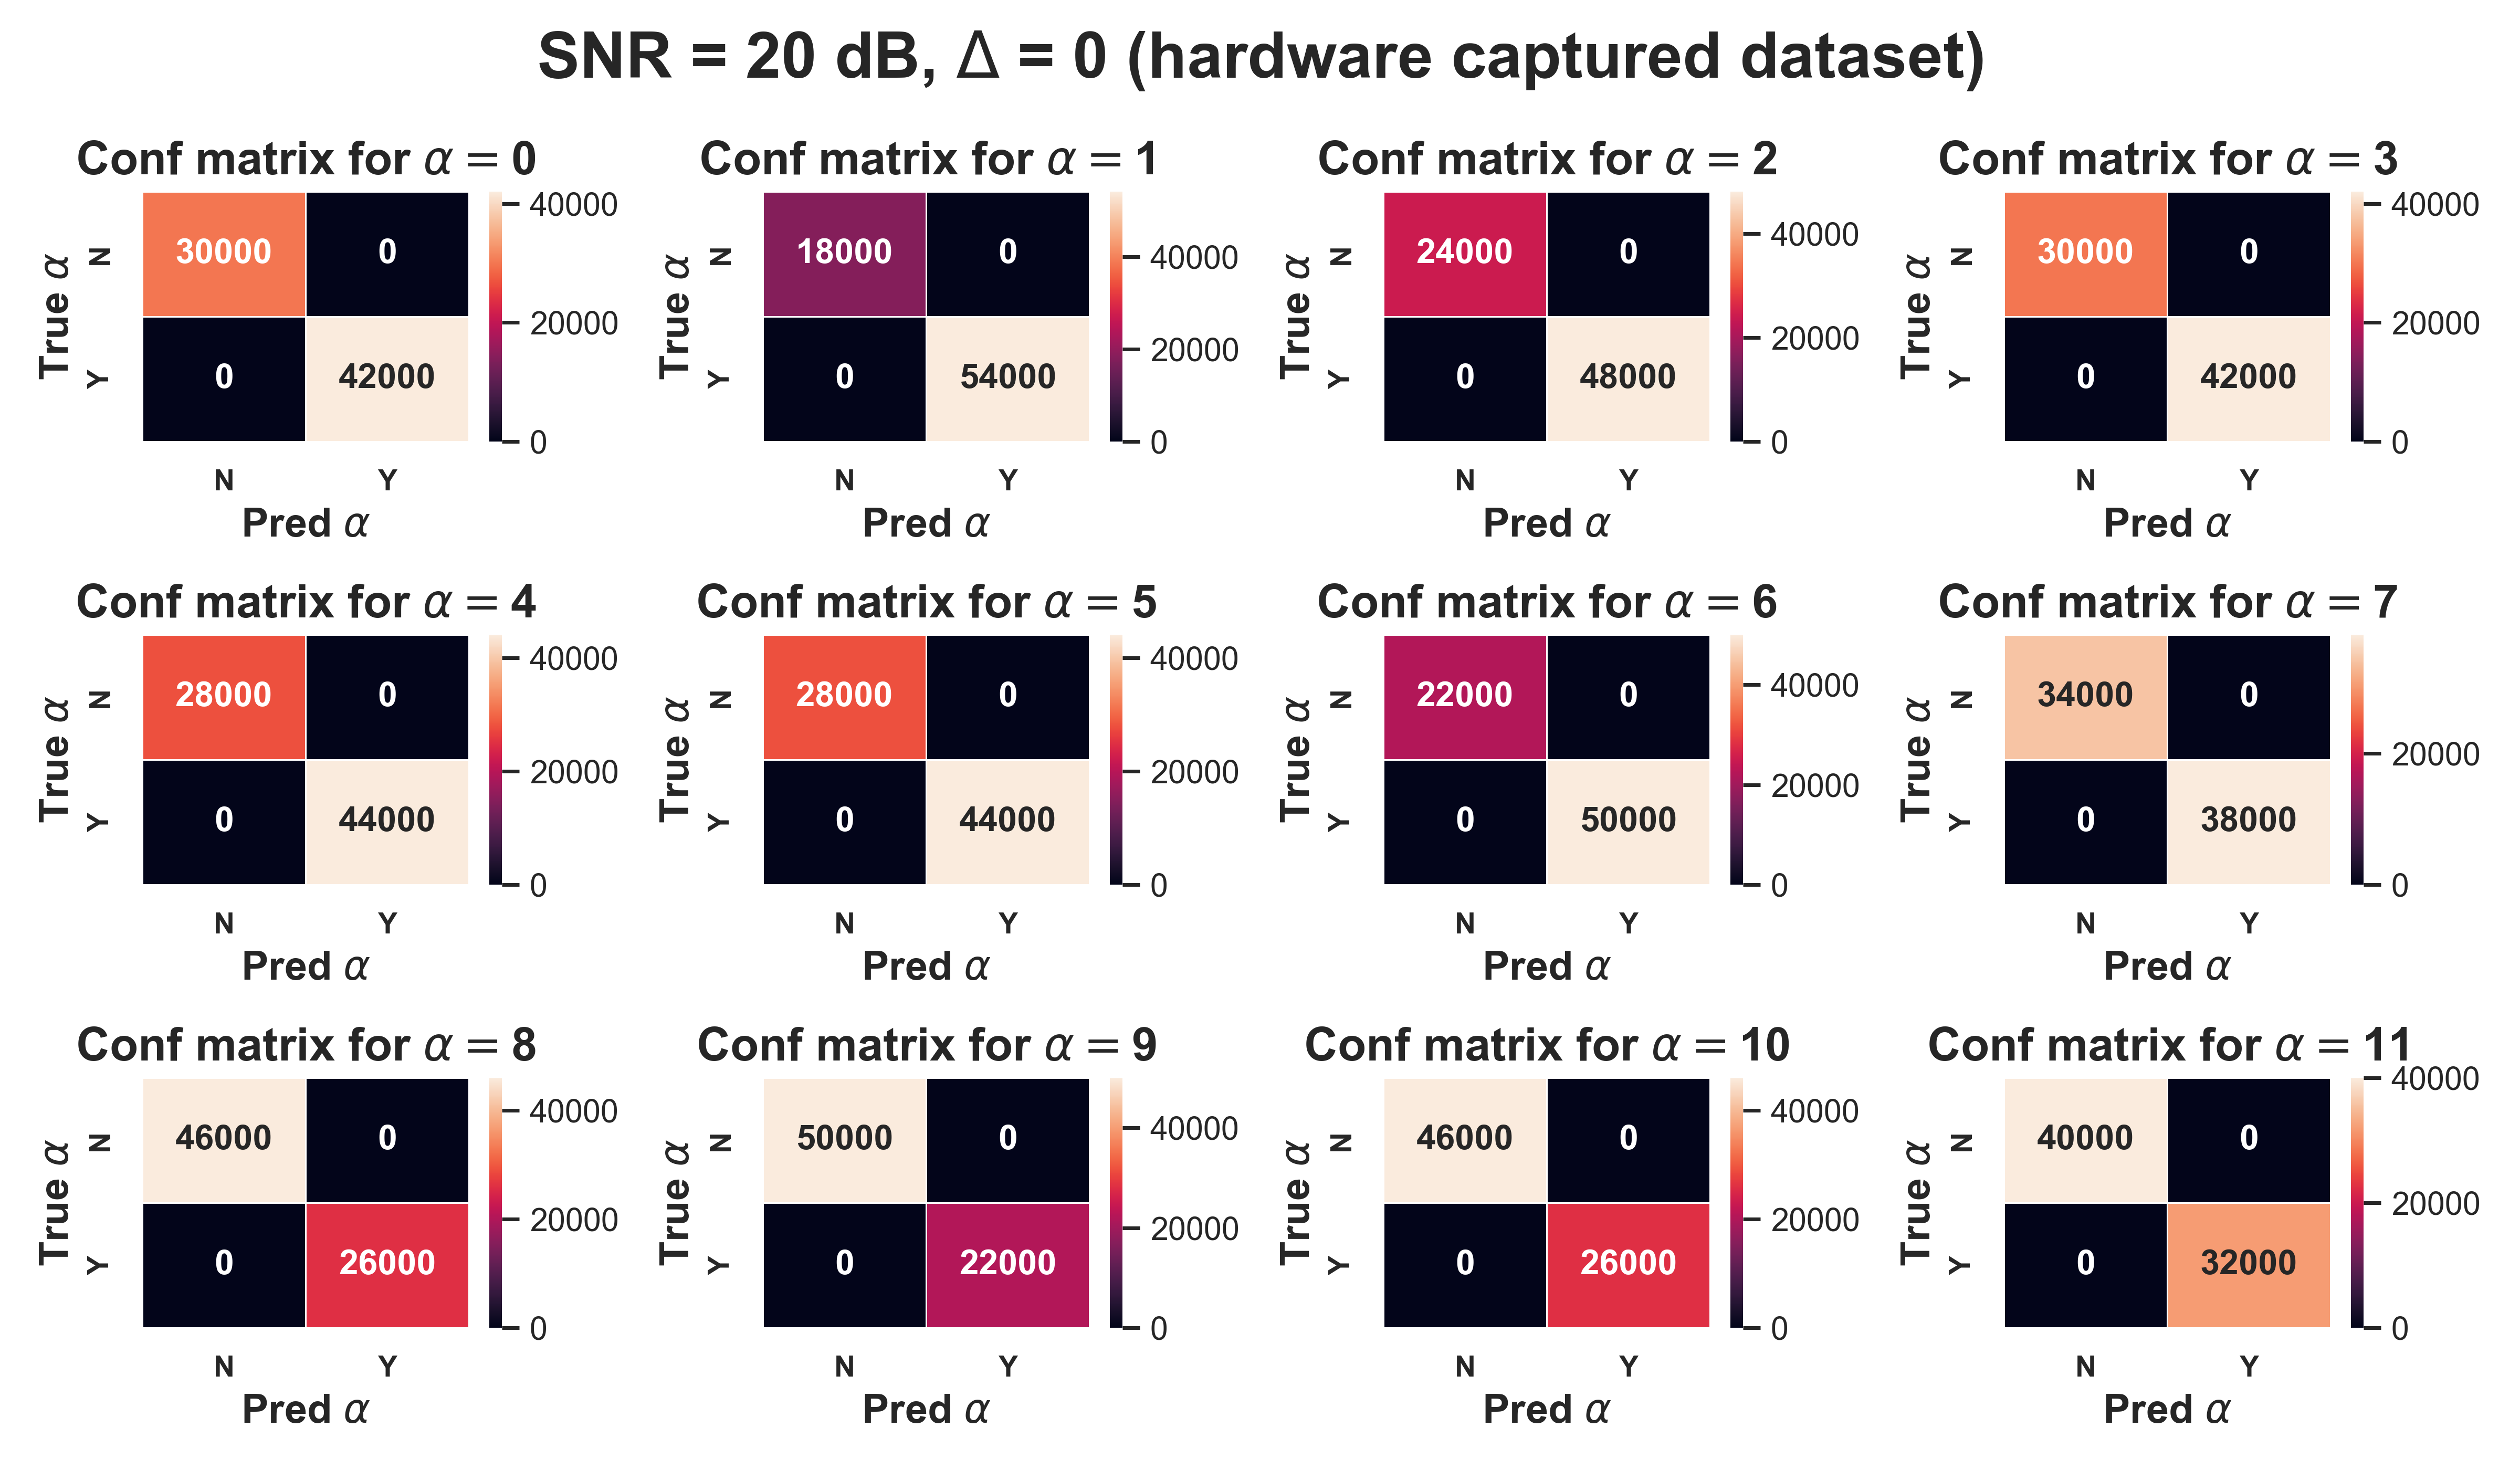
\includegraphics[width=\textwidth]{Figures/Conf_mtx_multi_label_SNR_20_dB_Max_off_0_train_sim_test_hw.png}
         \caption{}
         \label{fig: cm_multilabel_snr_20_off_0_hw}
     \end{subfigure}
        \caption{Multi-label confusion matrix at SNR = $20$ dB and $\Delta$ = $0$ for (a) simulated test dataset and (b) hardware captured test dataset. Here, $\alpha$ represents the UCI specific cyclic shift.}
        \label{fig: cm_multilabel_snr_20_off_0}
\end{figure}


\begin{figure}[ht!]
    \captionsetup{justification=justified}
     \centering
     \begin{subfigure}[b]{0.48\textwidth}
         \centering
         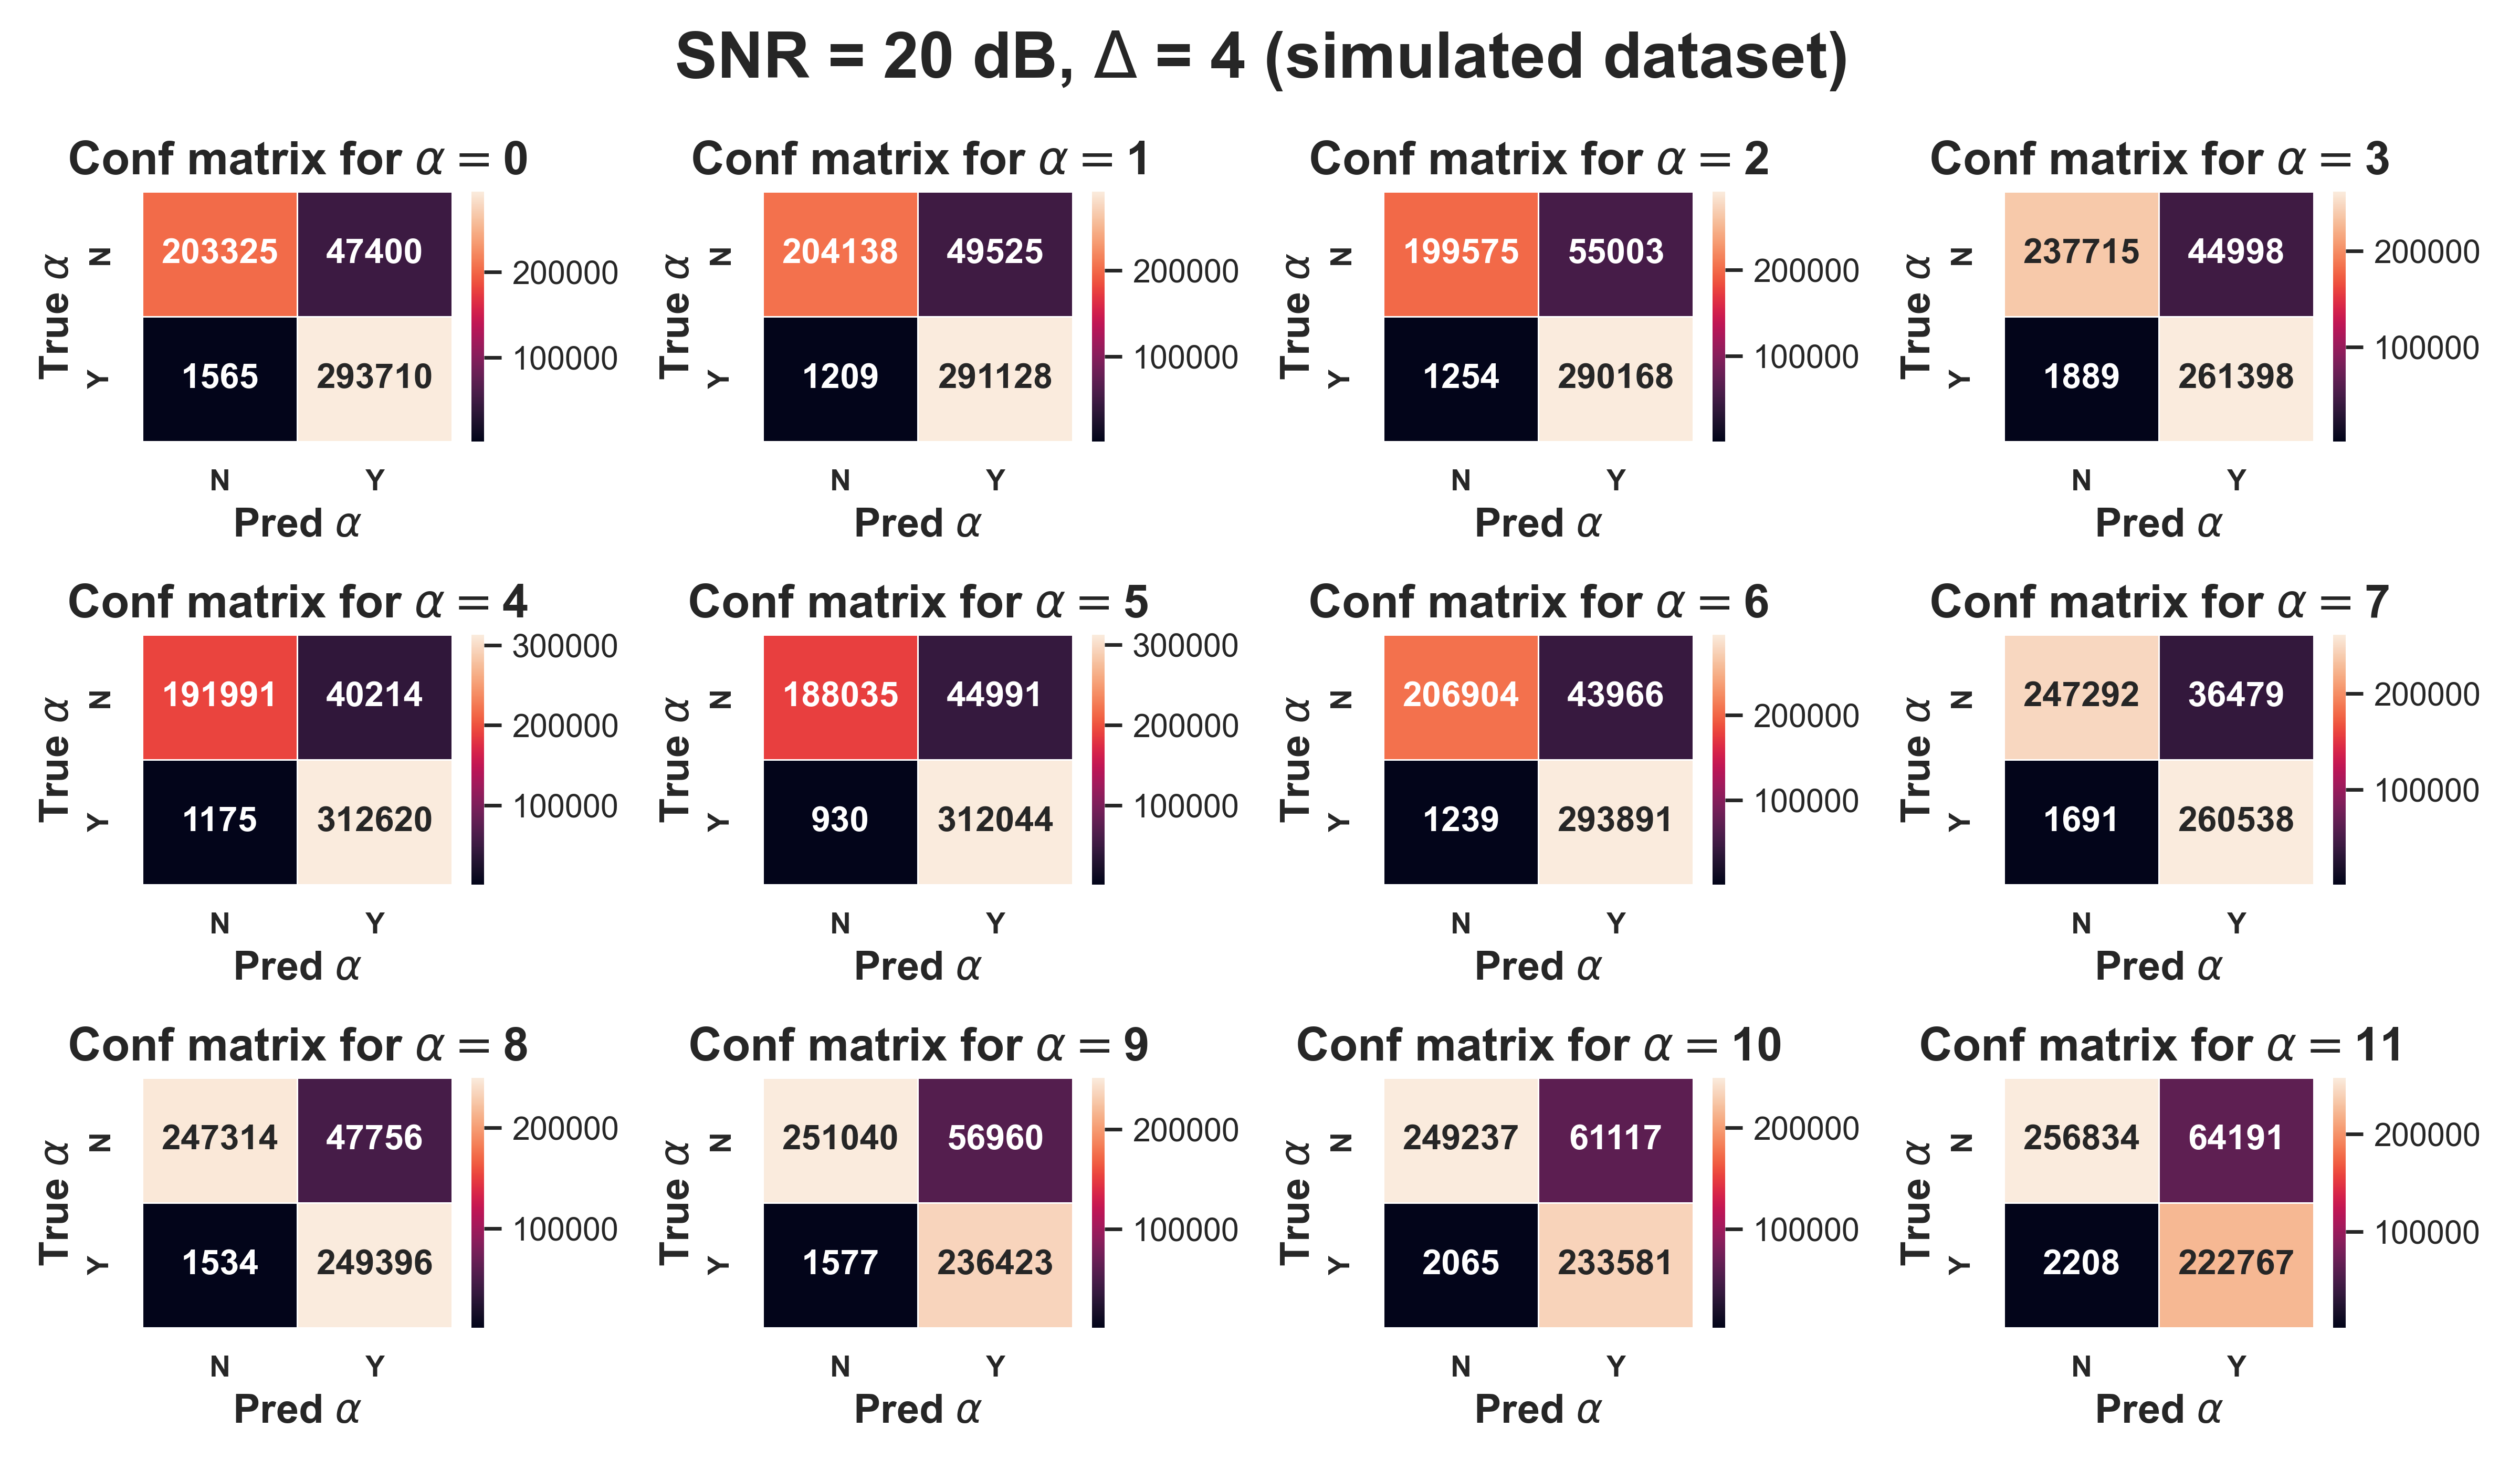
\includegraphics[width=\textwidth]{Figures/Conf_mtx_multi_label_SNR_20_dB_Max_off_4_train_sim_test_sim.png}
         \caption{}
         \label{fig: cm_multilabel_snr_20_off_4_sim}
     \end{subfigure}
     \\
     \begin{subfigure}[b]{0.48\textwidth}
         \centering
         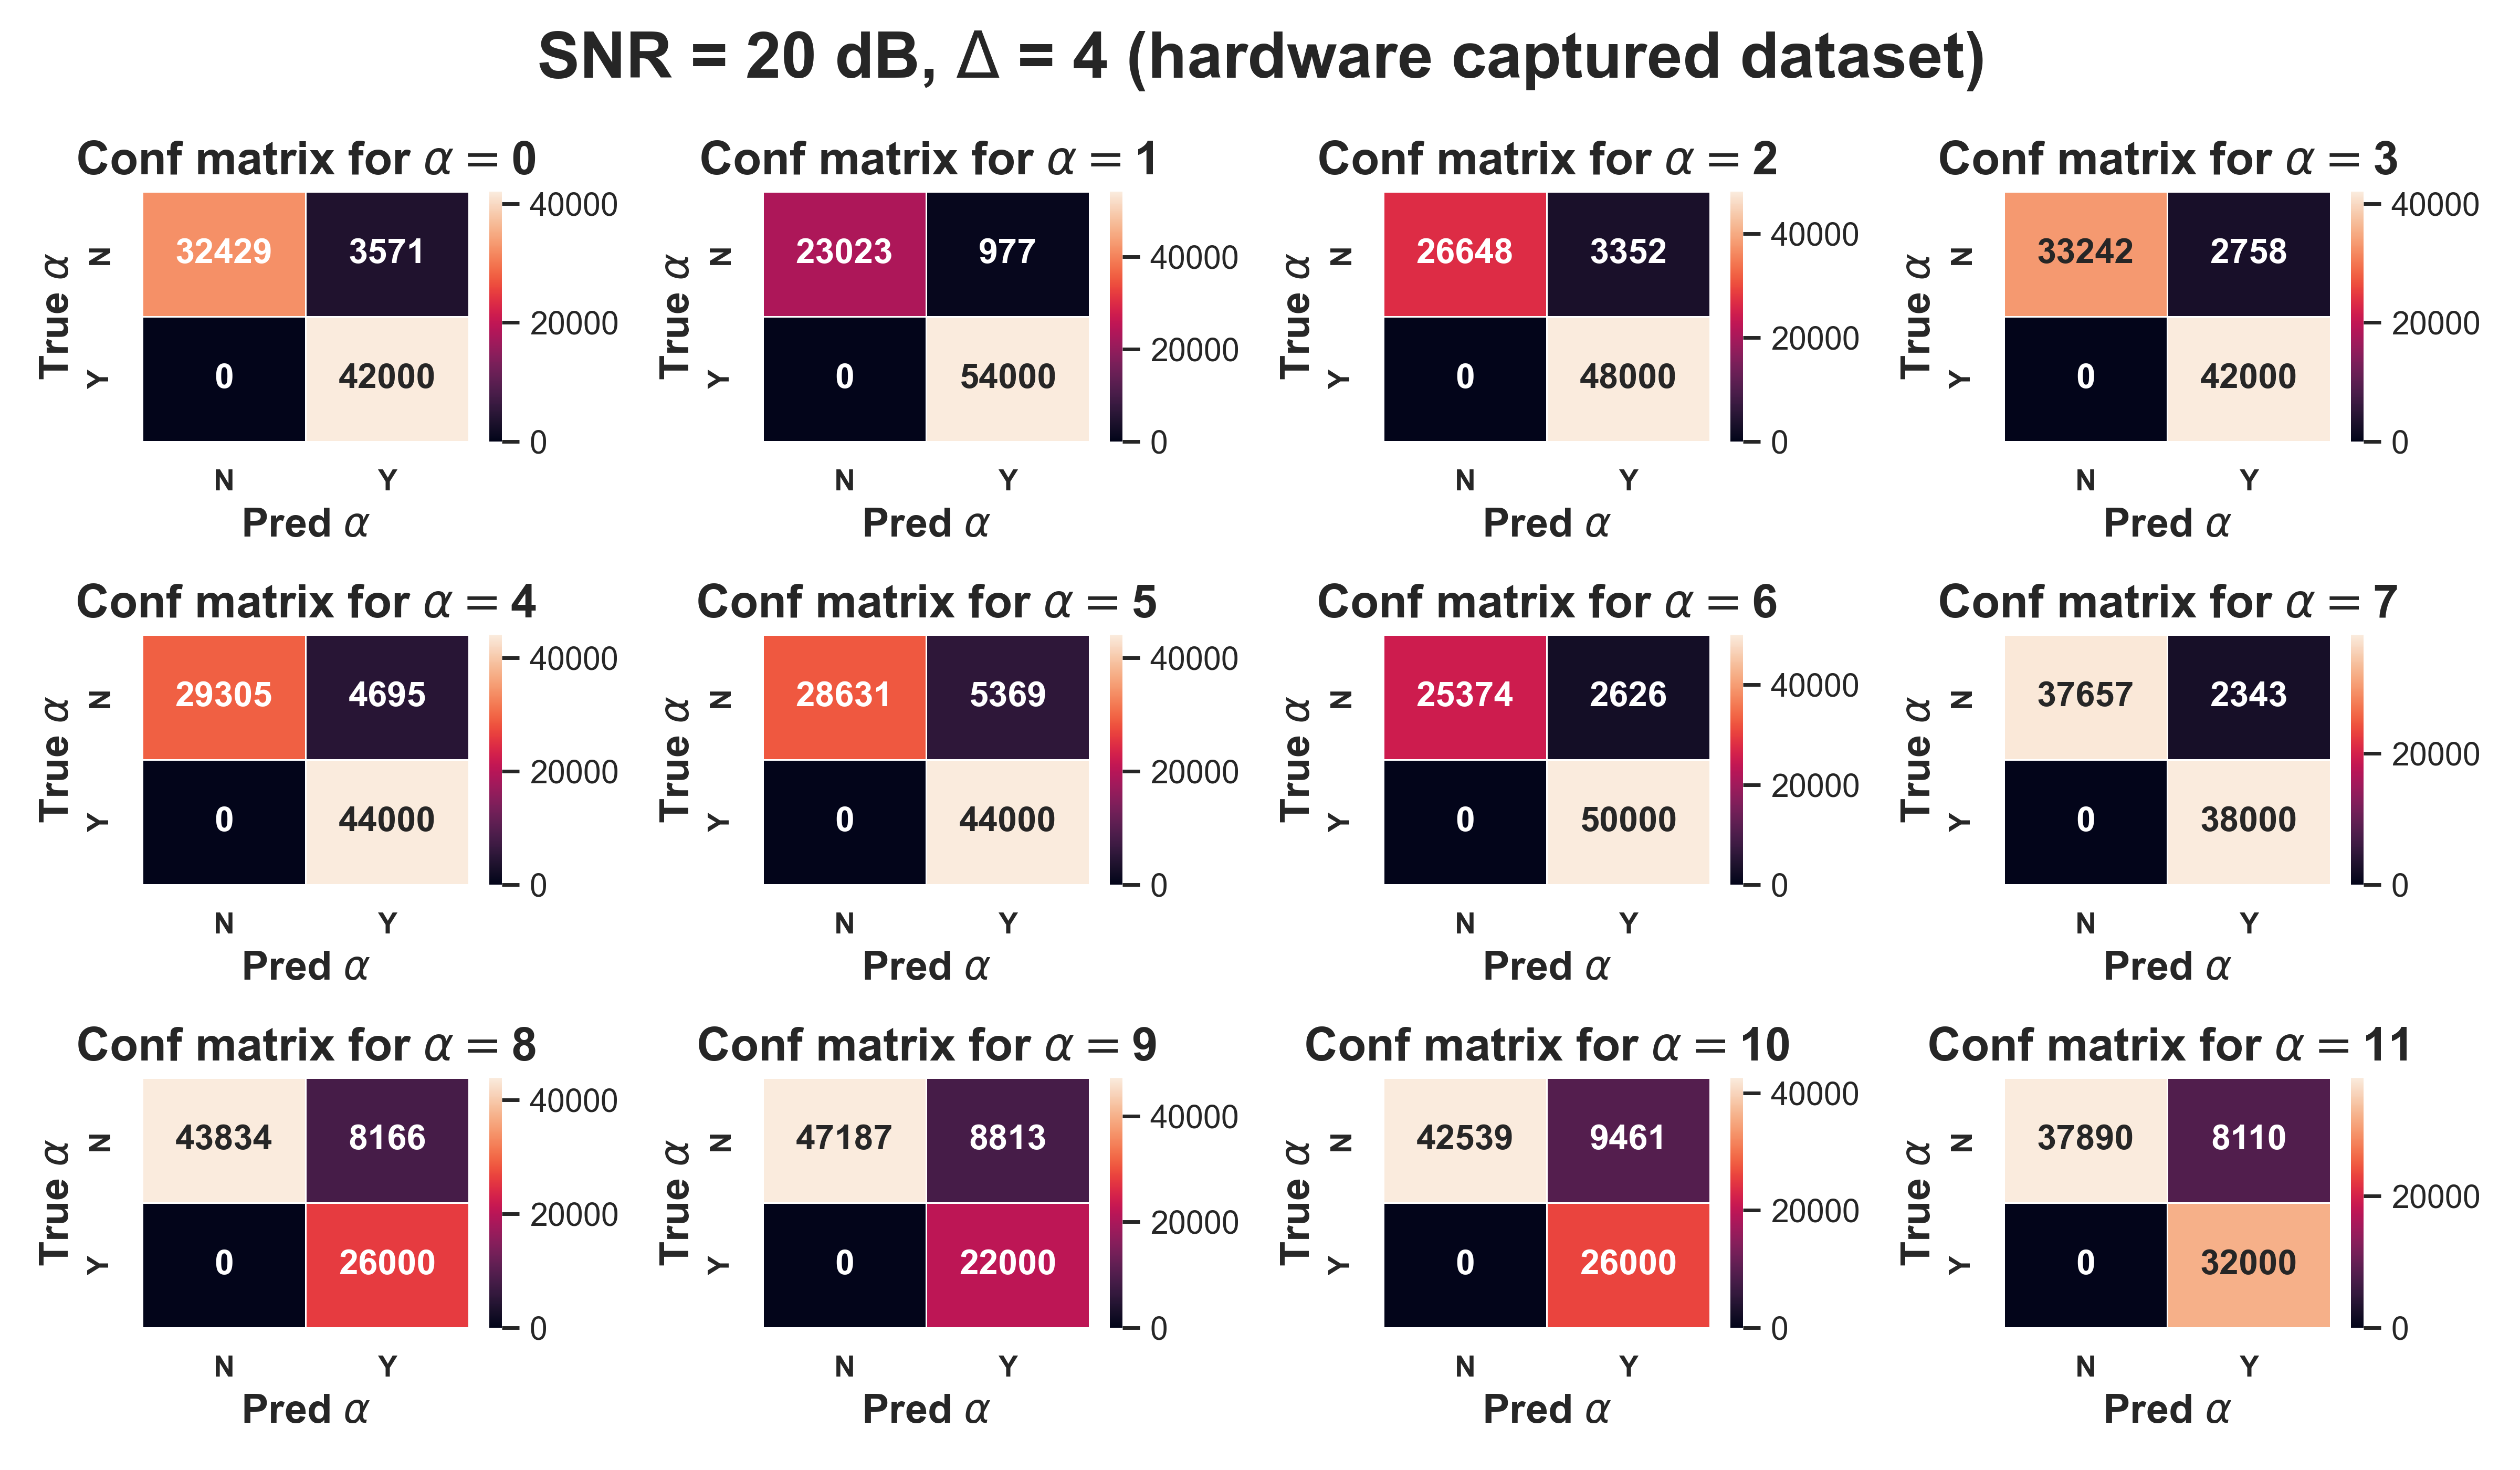
\includegraphics[width=\textwidth]{Figures/Conf_mtx_multi_label_SNR_20_dB_Max_off_4_train_sim_test_hw.png}
         \caption{}
         \label{fig: cm_multilabel_snr_20_off_4_hw}
     \end{subfigure}
        \caption{Multi-label confusion matrix at SNR = $20$ dB and $\Delta$ = $4$ for (a) simulated test dataset and (b) hardware captured test dataset.}
        \label{fig: cm_multilabel_snr_20_off_4}
\end{figure}

However, it should be noted that the multi-label confusion matrix does not show the exact details of misclassifications. To gain a deeper understanding of the mistakes made by the model, consider the matrices in Figures~\ref{fig: cm_num_UE_snr_0_off_0} to~\ref{fig: cm_num_UE_snr_20_off_4}. For each instance of the received PUCCH signal, there are two characteristics to correct classification. The first characteristic is correctly identifying the number of multiplexed UEs ($N_{UE}$) embedded in the signal. Even though this is not an explicit output of the NN model, we believe that the model is learning to estimate the number of multiplexed UEs. Our belief is based on the fact that when the number of possible multiplexed UEs is not given as metadata to NN input, the accuracy drops significantly. The second characteristic of correct classification is derived from the explicit output of the NN model, which is the correct prediction of the value of $\alpha$ for each of the multiplexed UEs. 

Figures~\ref{fig: cm_num_UE_snr_0_off_0} and ~\ref{fig: cm_num_UE_snr_0_off_4} show confusion matrices for the number of multiplexed UEs for both simulated data and hardware-captured data at an SNR of $0$ dB and $\Delta$ values of $0$ and $4$ respectively. Figures~\ref{fig: cm_num_UE_snr_20_off_0} and ~\ref{fig: cm_num_UE_snr_20_off_4} confusion matrices for the number of multiplexed UEs for both simulated data and hardware-captured data at an SNR of $20$ dB and $\Delta$ values of $0$ and $4$ respectively. We notice that all the confusion matrices for the prediction of the number of multiplexed UEs are largely diagonally dominant. Furthermore, for any SNR, when $\Delta = 0$, the error in the predicted number of UEs fluctuates between +1 and -1 in the majority of instances, confirming the high accuracy values in Figure~\ref{fig: acc_vs_snr}. As $\Delta$ increases,  the error tends to grow on the positive side, meaning that the NN model predicts more UEs than actually present. As stated above, the overprediction is because $\Delta$ is always positive. 

\begin{figure}[ht!]
    \captionsetup{justification=justified}
     \centering
     \begin{subfigure}[b]{0.48\textwidth}
         \centering
         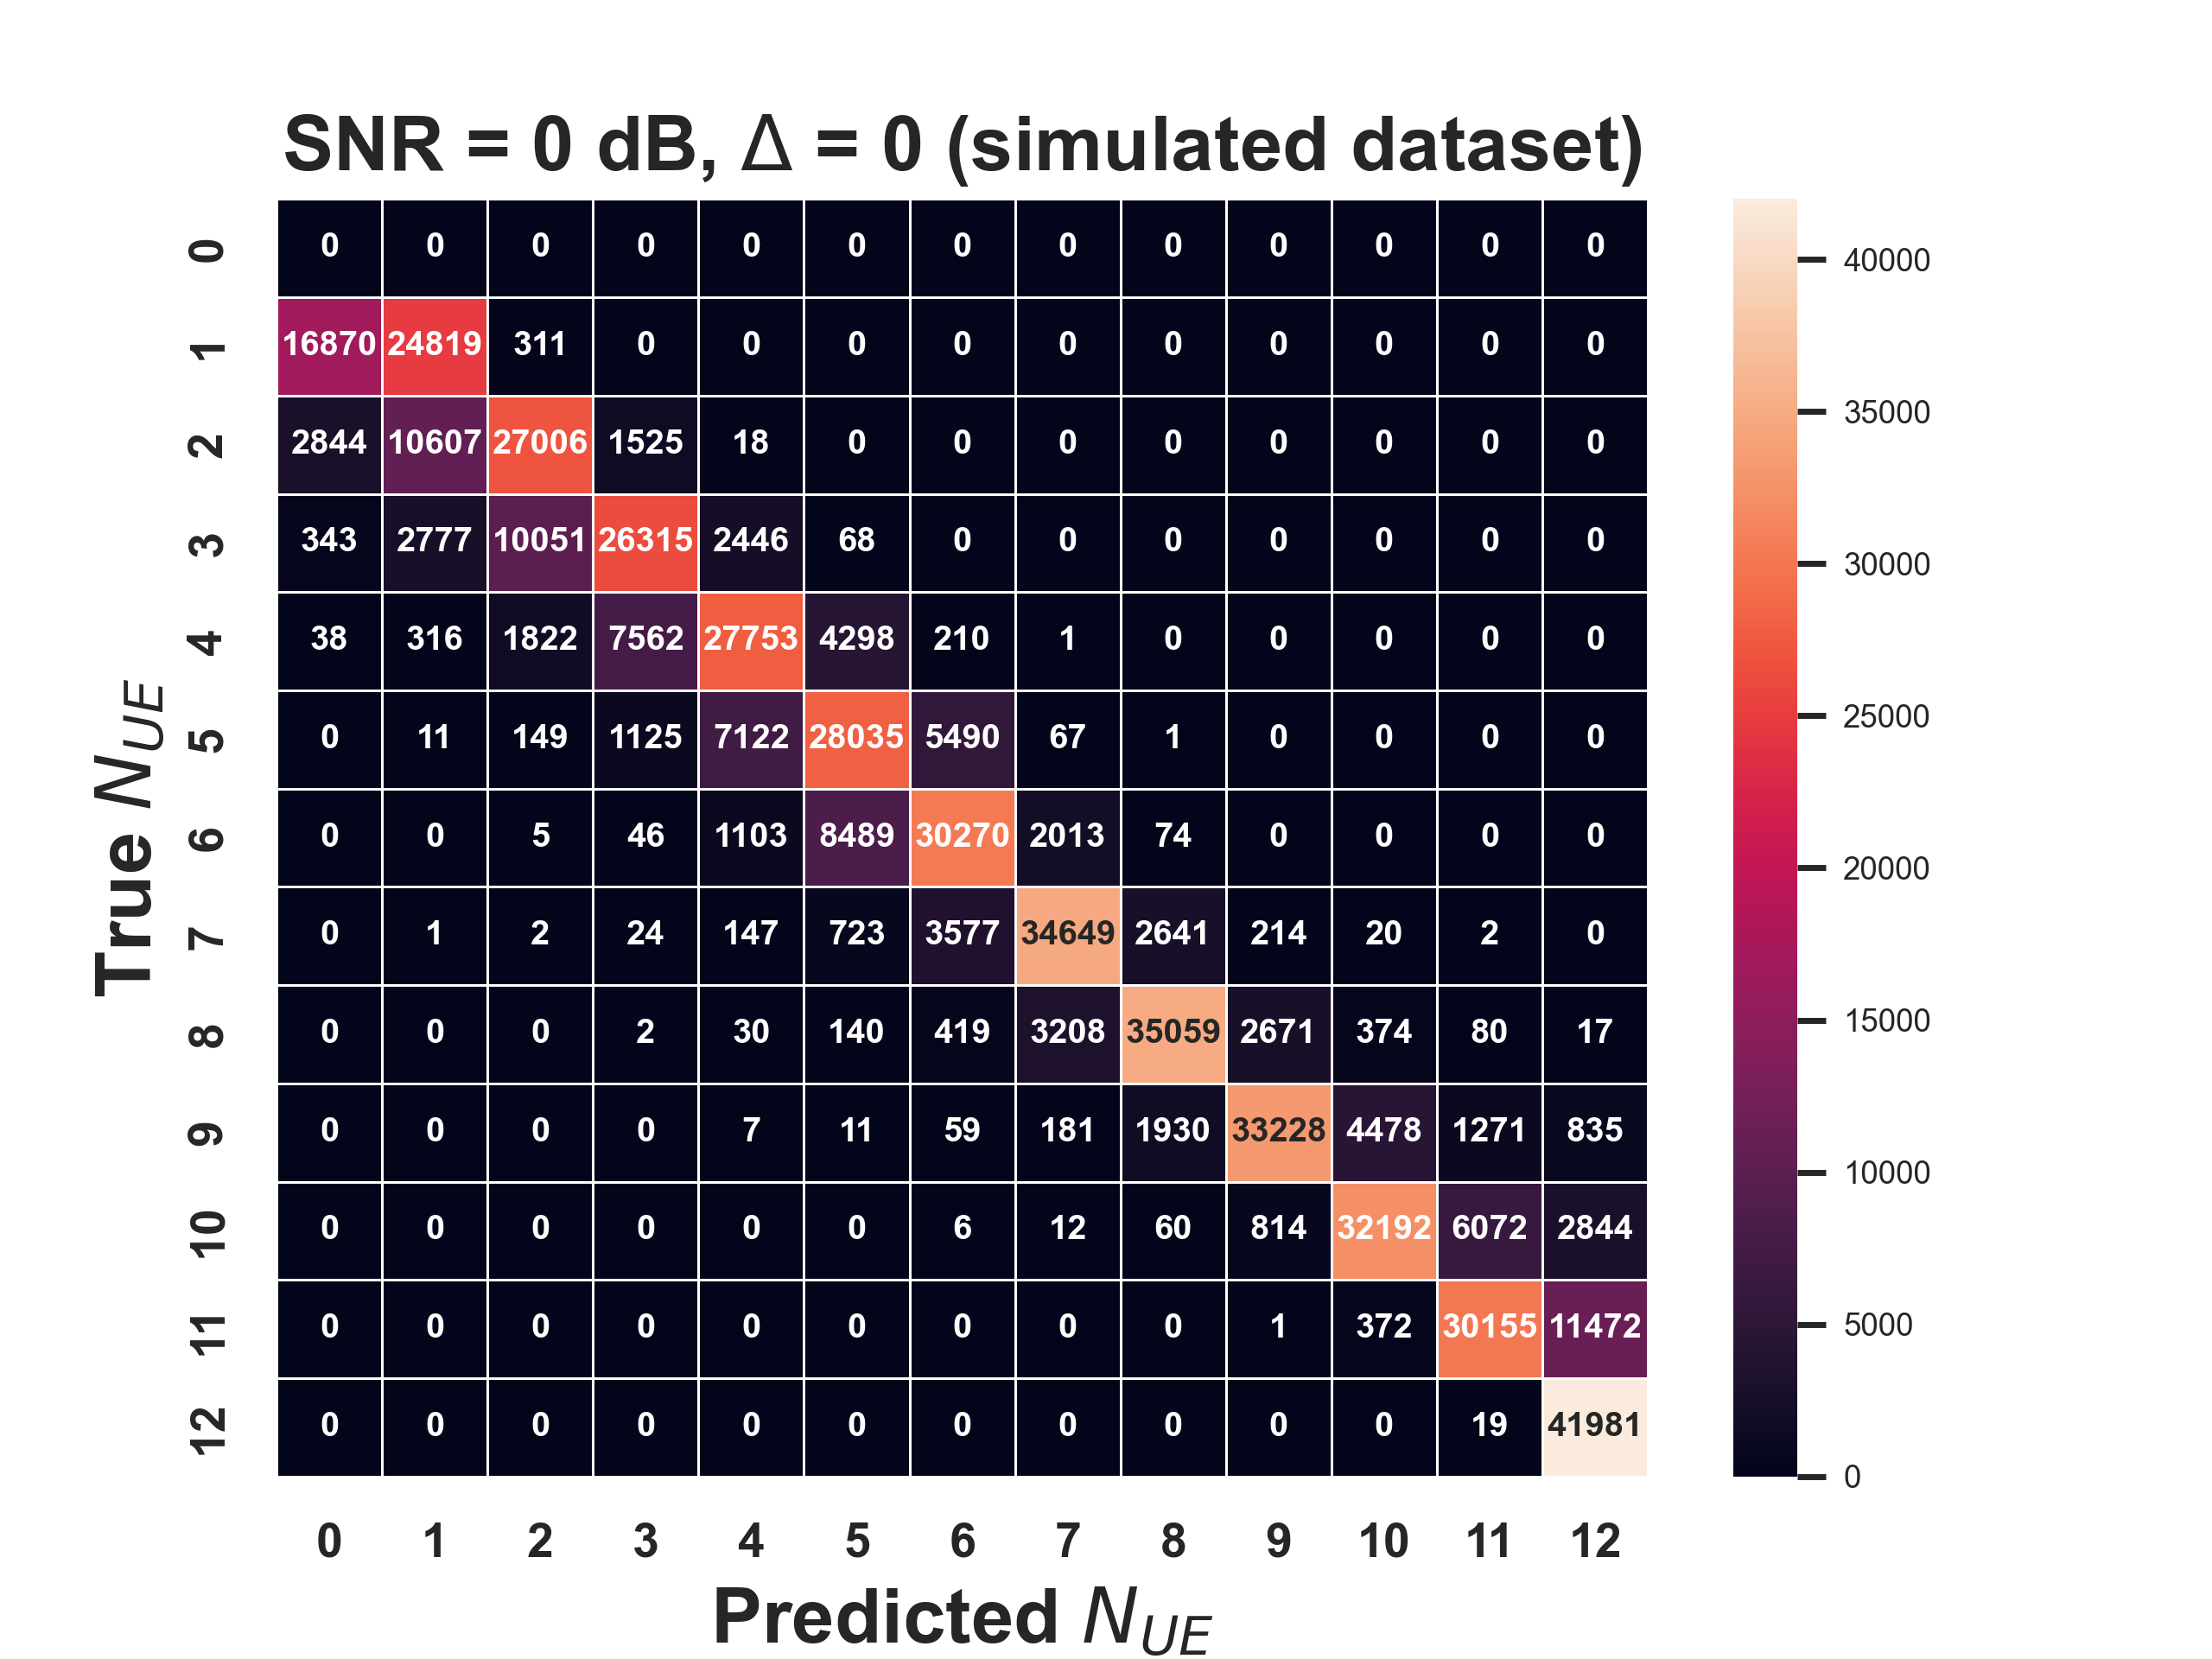
\includegraphics[width=\textwidth]{Figures/Conf_mtx_num_UEs_SNR_0_dB_Max_off_0_train_sim_test_sim.png}
         \caption{}
         \label{fig: cm_num_UE_snr_0_off_0_sim}
     \end{subfigure}
     \\
     \begin{subfigure}[b]{0.48\textwidth}
         \centering
         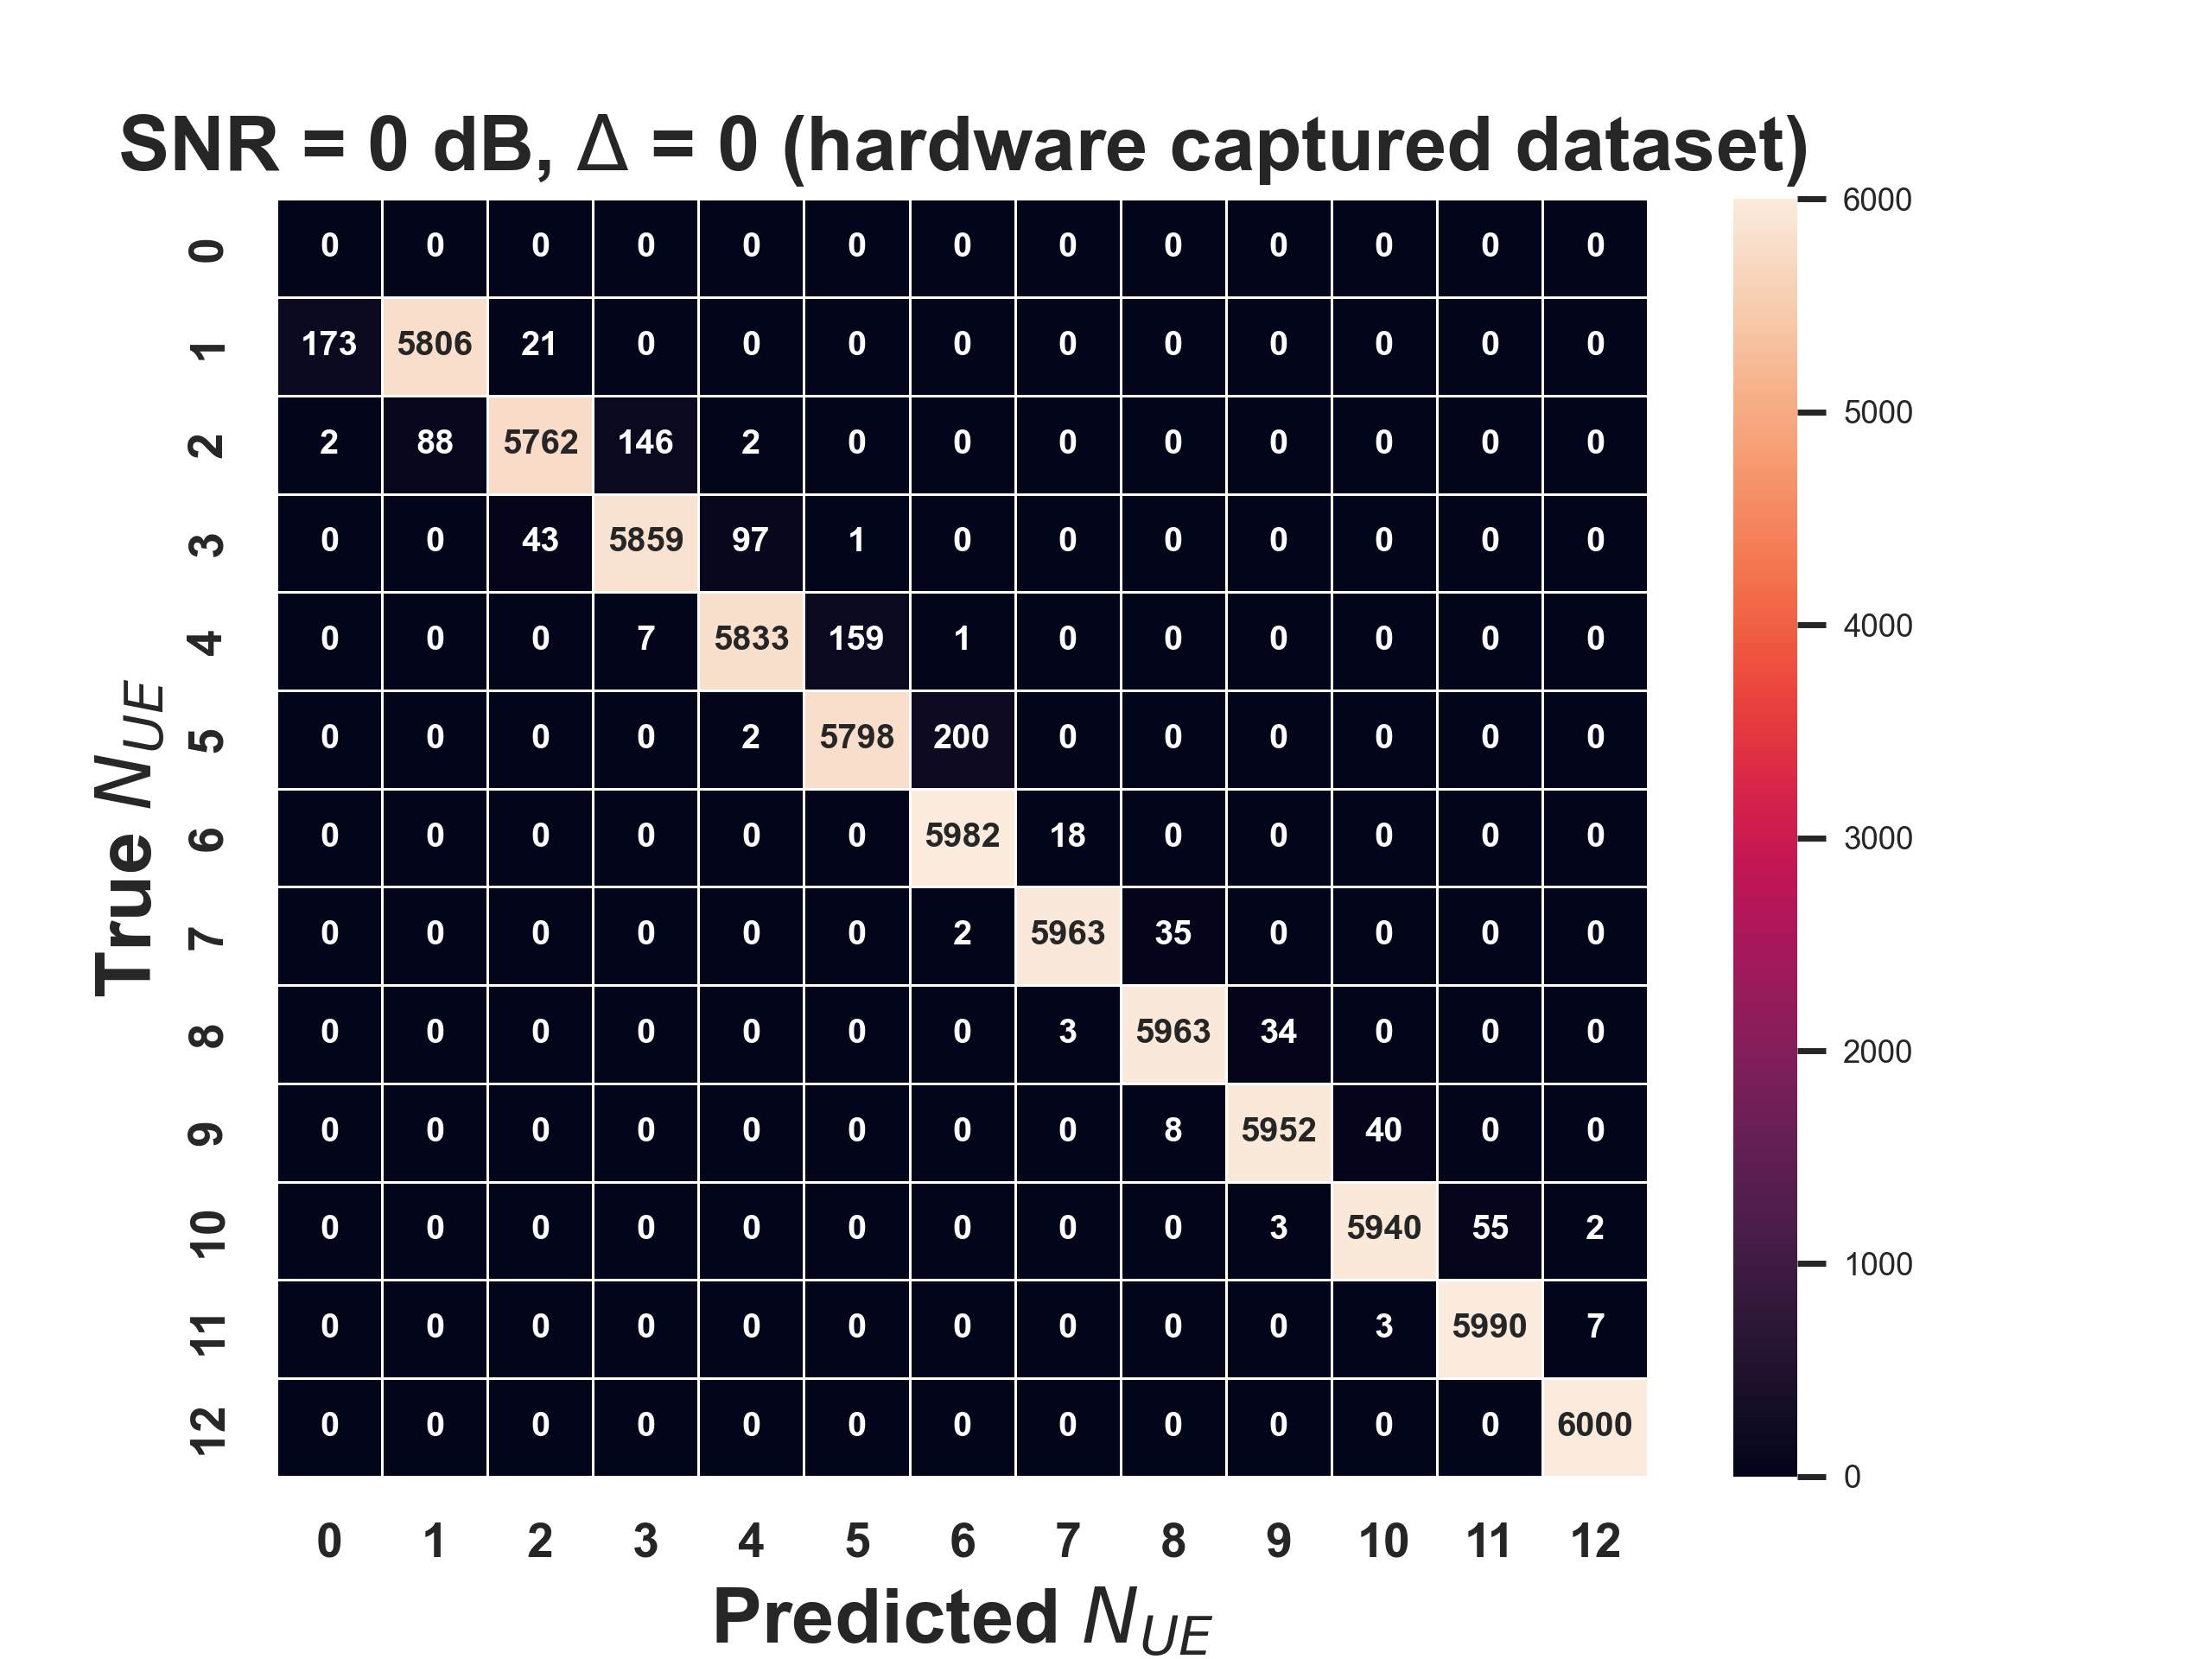
\includegraphics[width=\textwidth]{Figures/Conf_mtx_num_UEs_SNR_0_dB_Max_off_0_train_sim_test_hw.png}
         \caption{}
         \label{fig: cm_num_UE_snr_0_off_0_hw}
     \end{subfigure}
        \caption{Confusion matrix for the number of multiplexed UEs $N_{UE}$, at SNR = $0$ dB and $\Delta$ = $0$ for (a) simulated test dataset and (b) hardware captured test dataset.}
        \label{fig: cm_num_UE_snr_0_off_0}
\end{figure}

\begin{figure}[ht!]
    \captionsetup{justification=justified}
     \centering
     \begin{subfigure}[b]{0.48\textwidth}
         \centering
         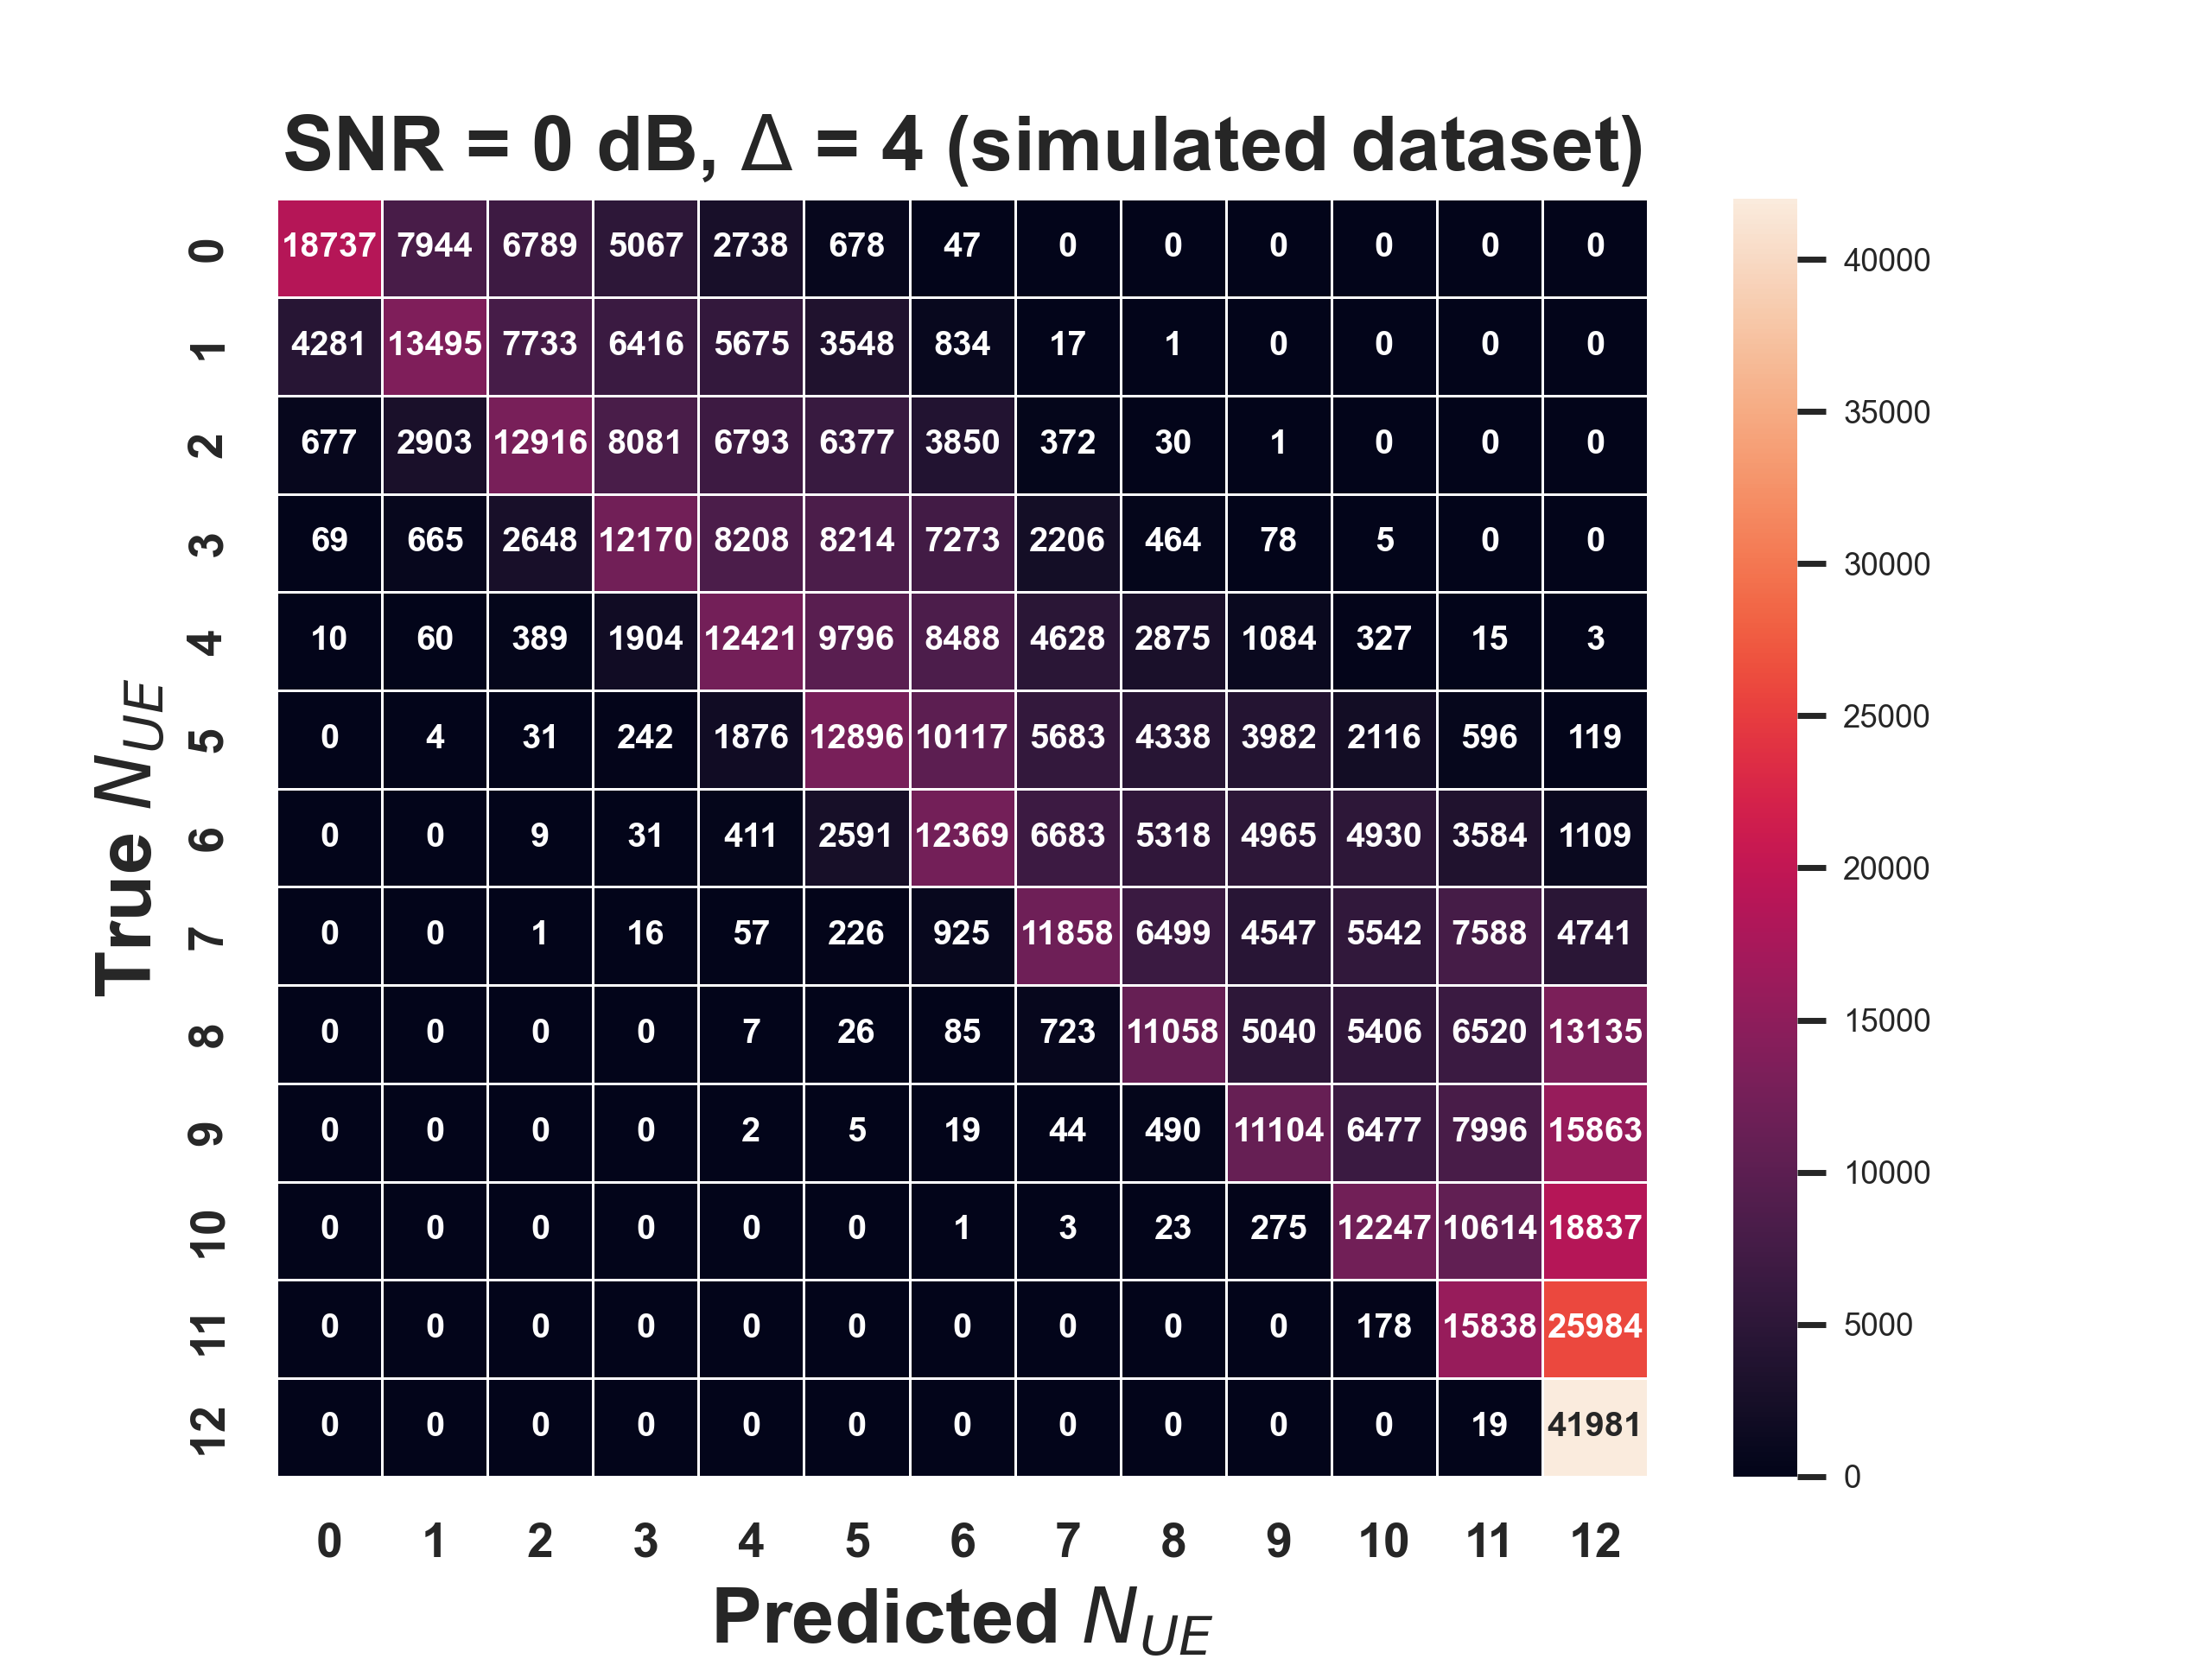
\includegraphics[width=\textwidth]{Figures/Conf_mtx_num_UEs_SNR_0_dB_Max_off_4_train_sim_test_sim.png}
         \caption{}
         \label{fig: cm_num_UE_snr_0_off_4_sim}
     \end{subfigure}
     \\
     \begin{subfigure}[b]{0.48\textwidth}
         \centering
         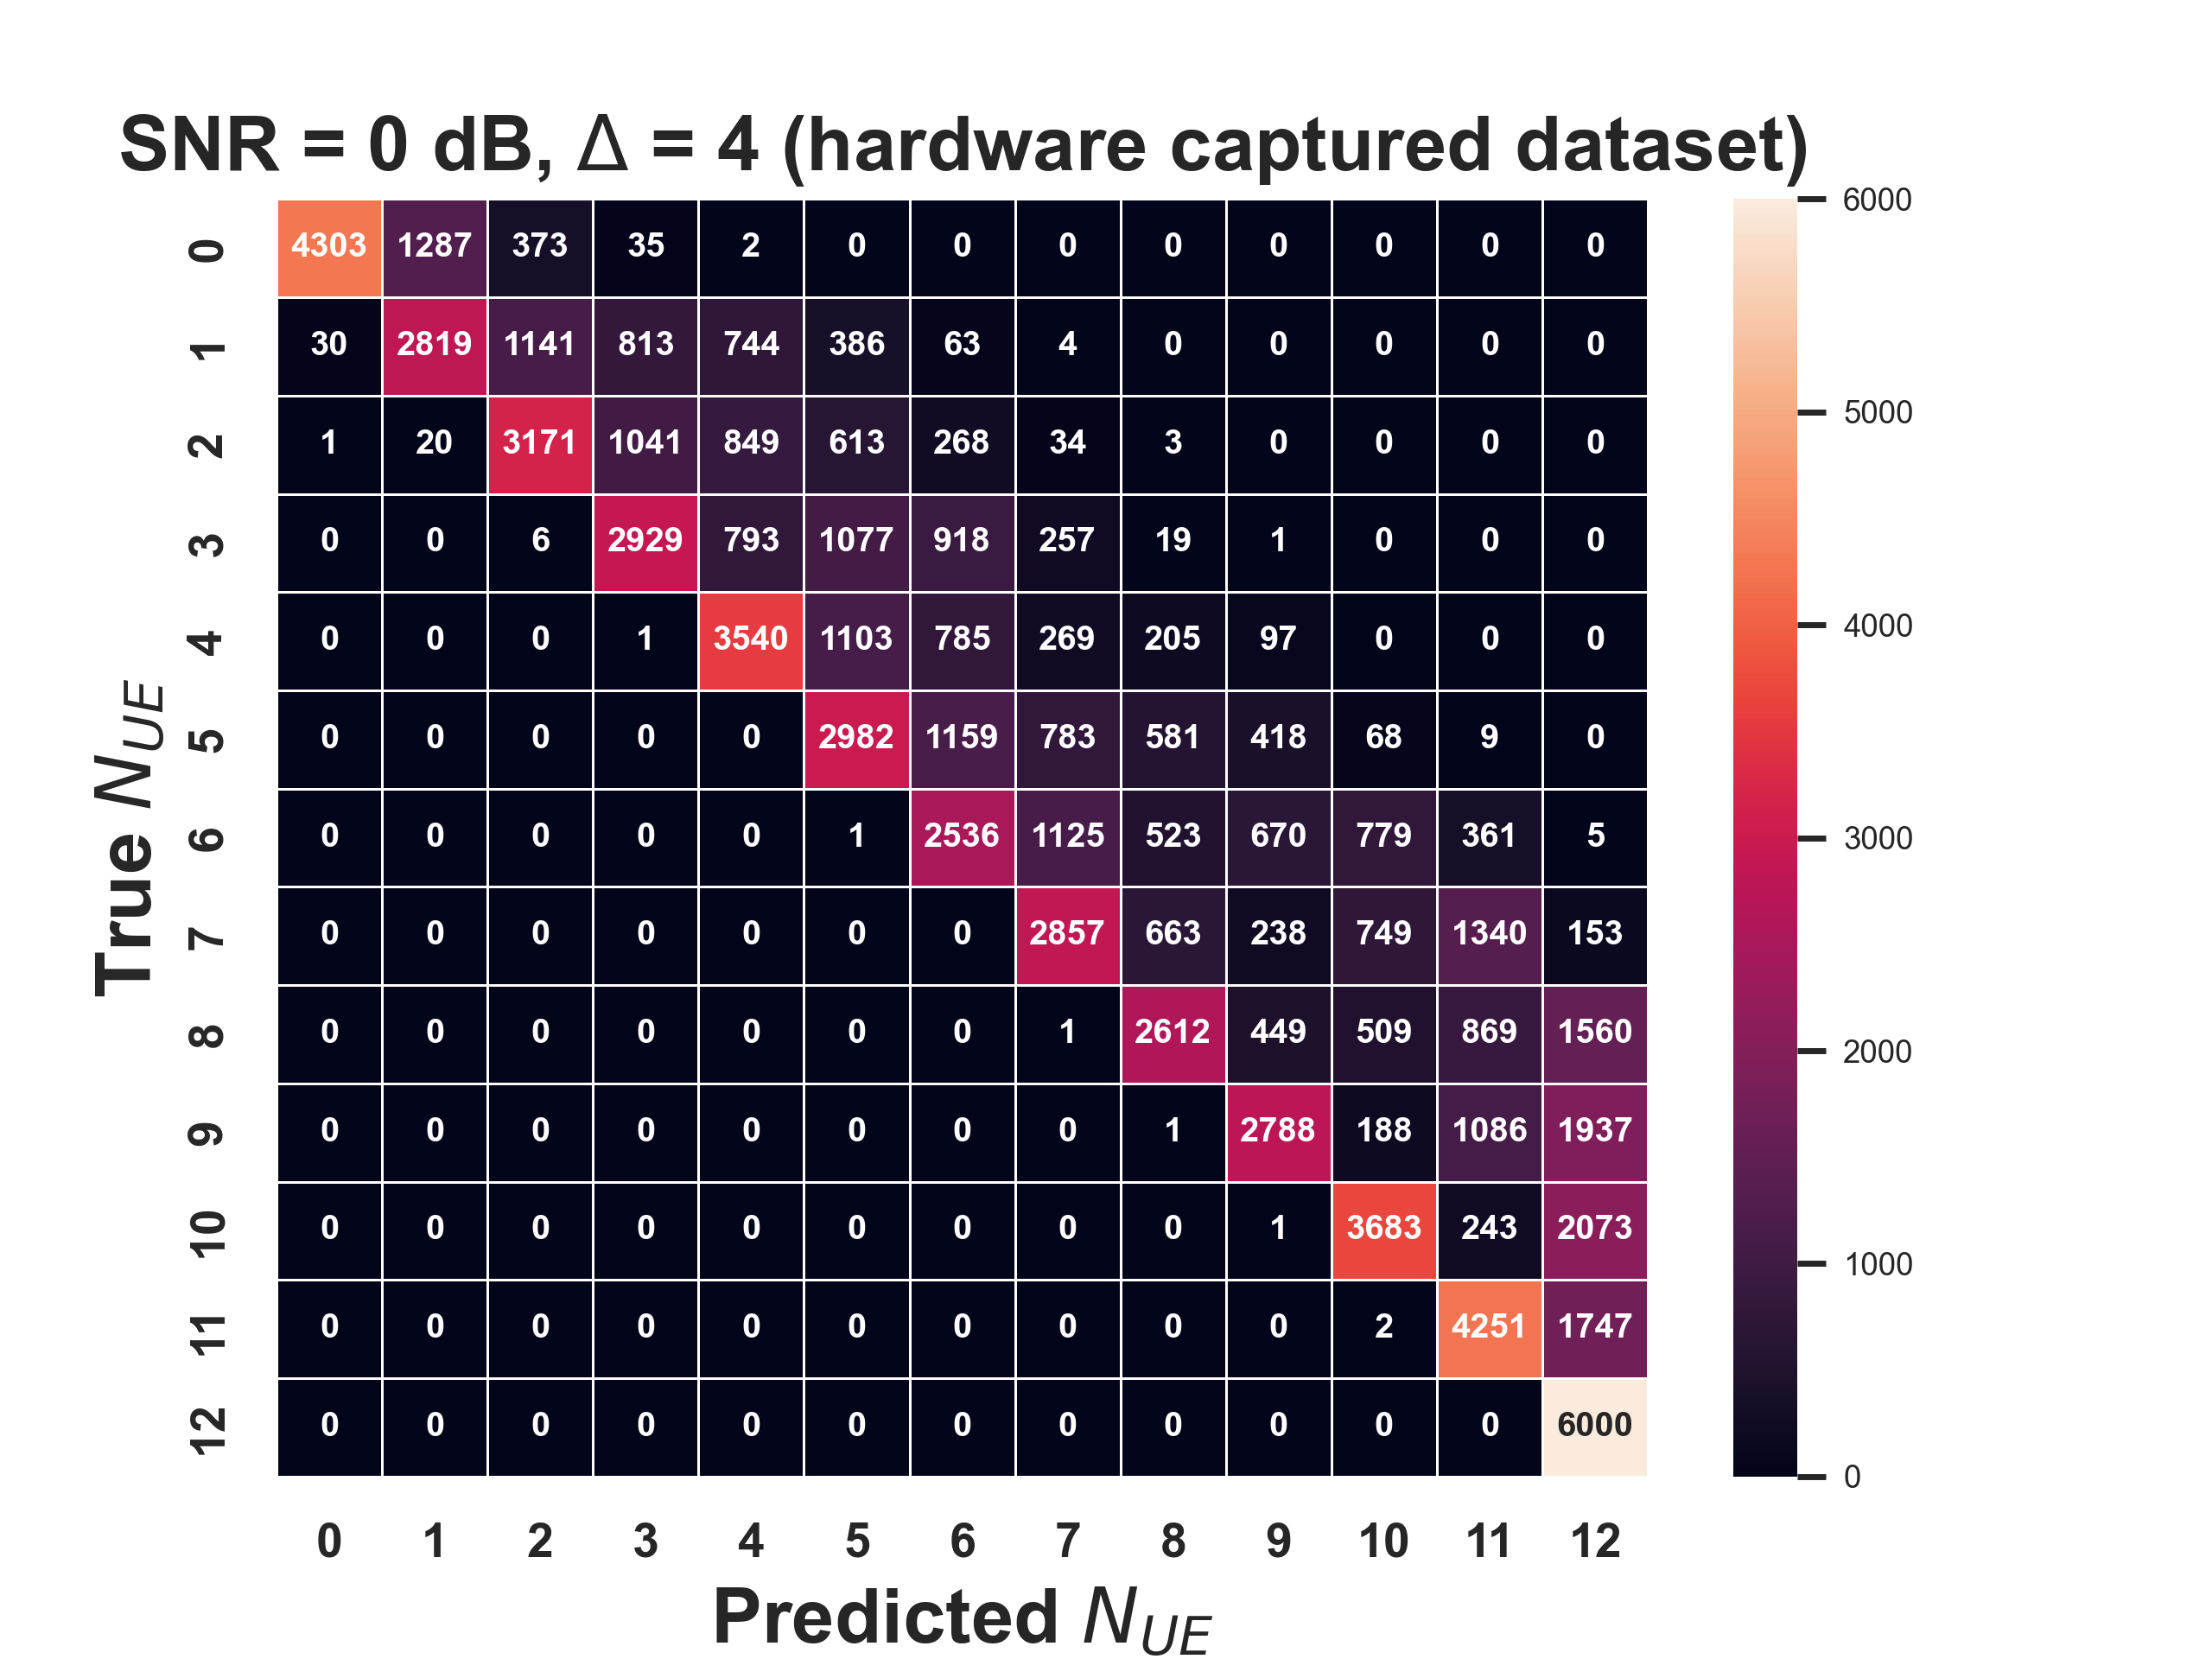
\includegraphics[width=\textwidth]{Figures/Conf_mtx_num_UEs_SNR_0_dB_Max_off_4_train_sim_test_hw.png}
         \caption{}
         \label{fig: cm_num_UE_snr_0_off_4_hw}
     \end{subfigure}
        \caption{Confusion matrix for the number of multiplexed UEs $N_{UE}$, at SNR = $0$ dB and $\Delta$ = $4$ for (a) simulated test dataset and (b) hardware captured test dataset.}
        \label{fig: cm_num_UE_snr_0_off_4}
\end{figure}

%%%%%%%%%%%

\begin{figure}[ht!]
    \captionsetup{justification=justified}
     \centering
     \begin{subfigure}[b]{0.48\textwidth}
         \centering
         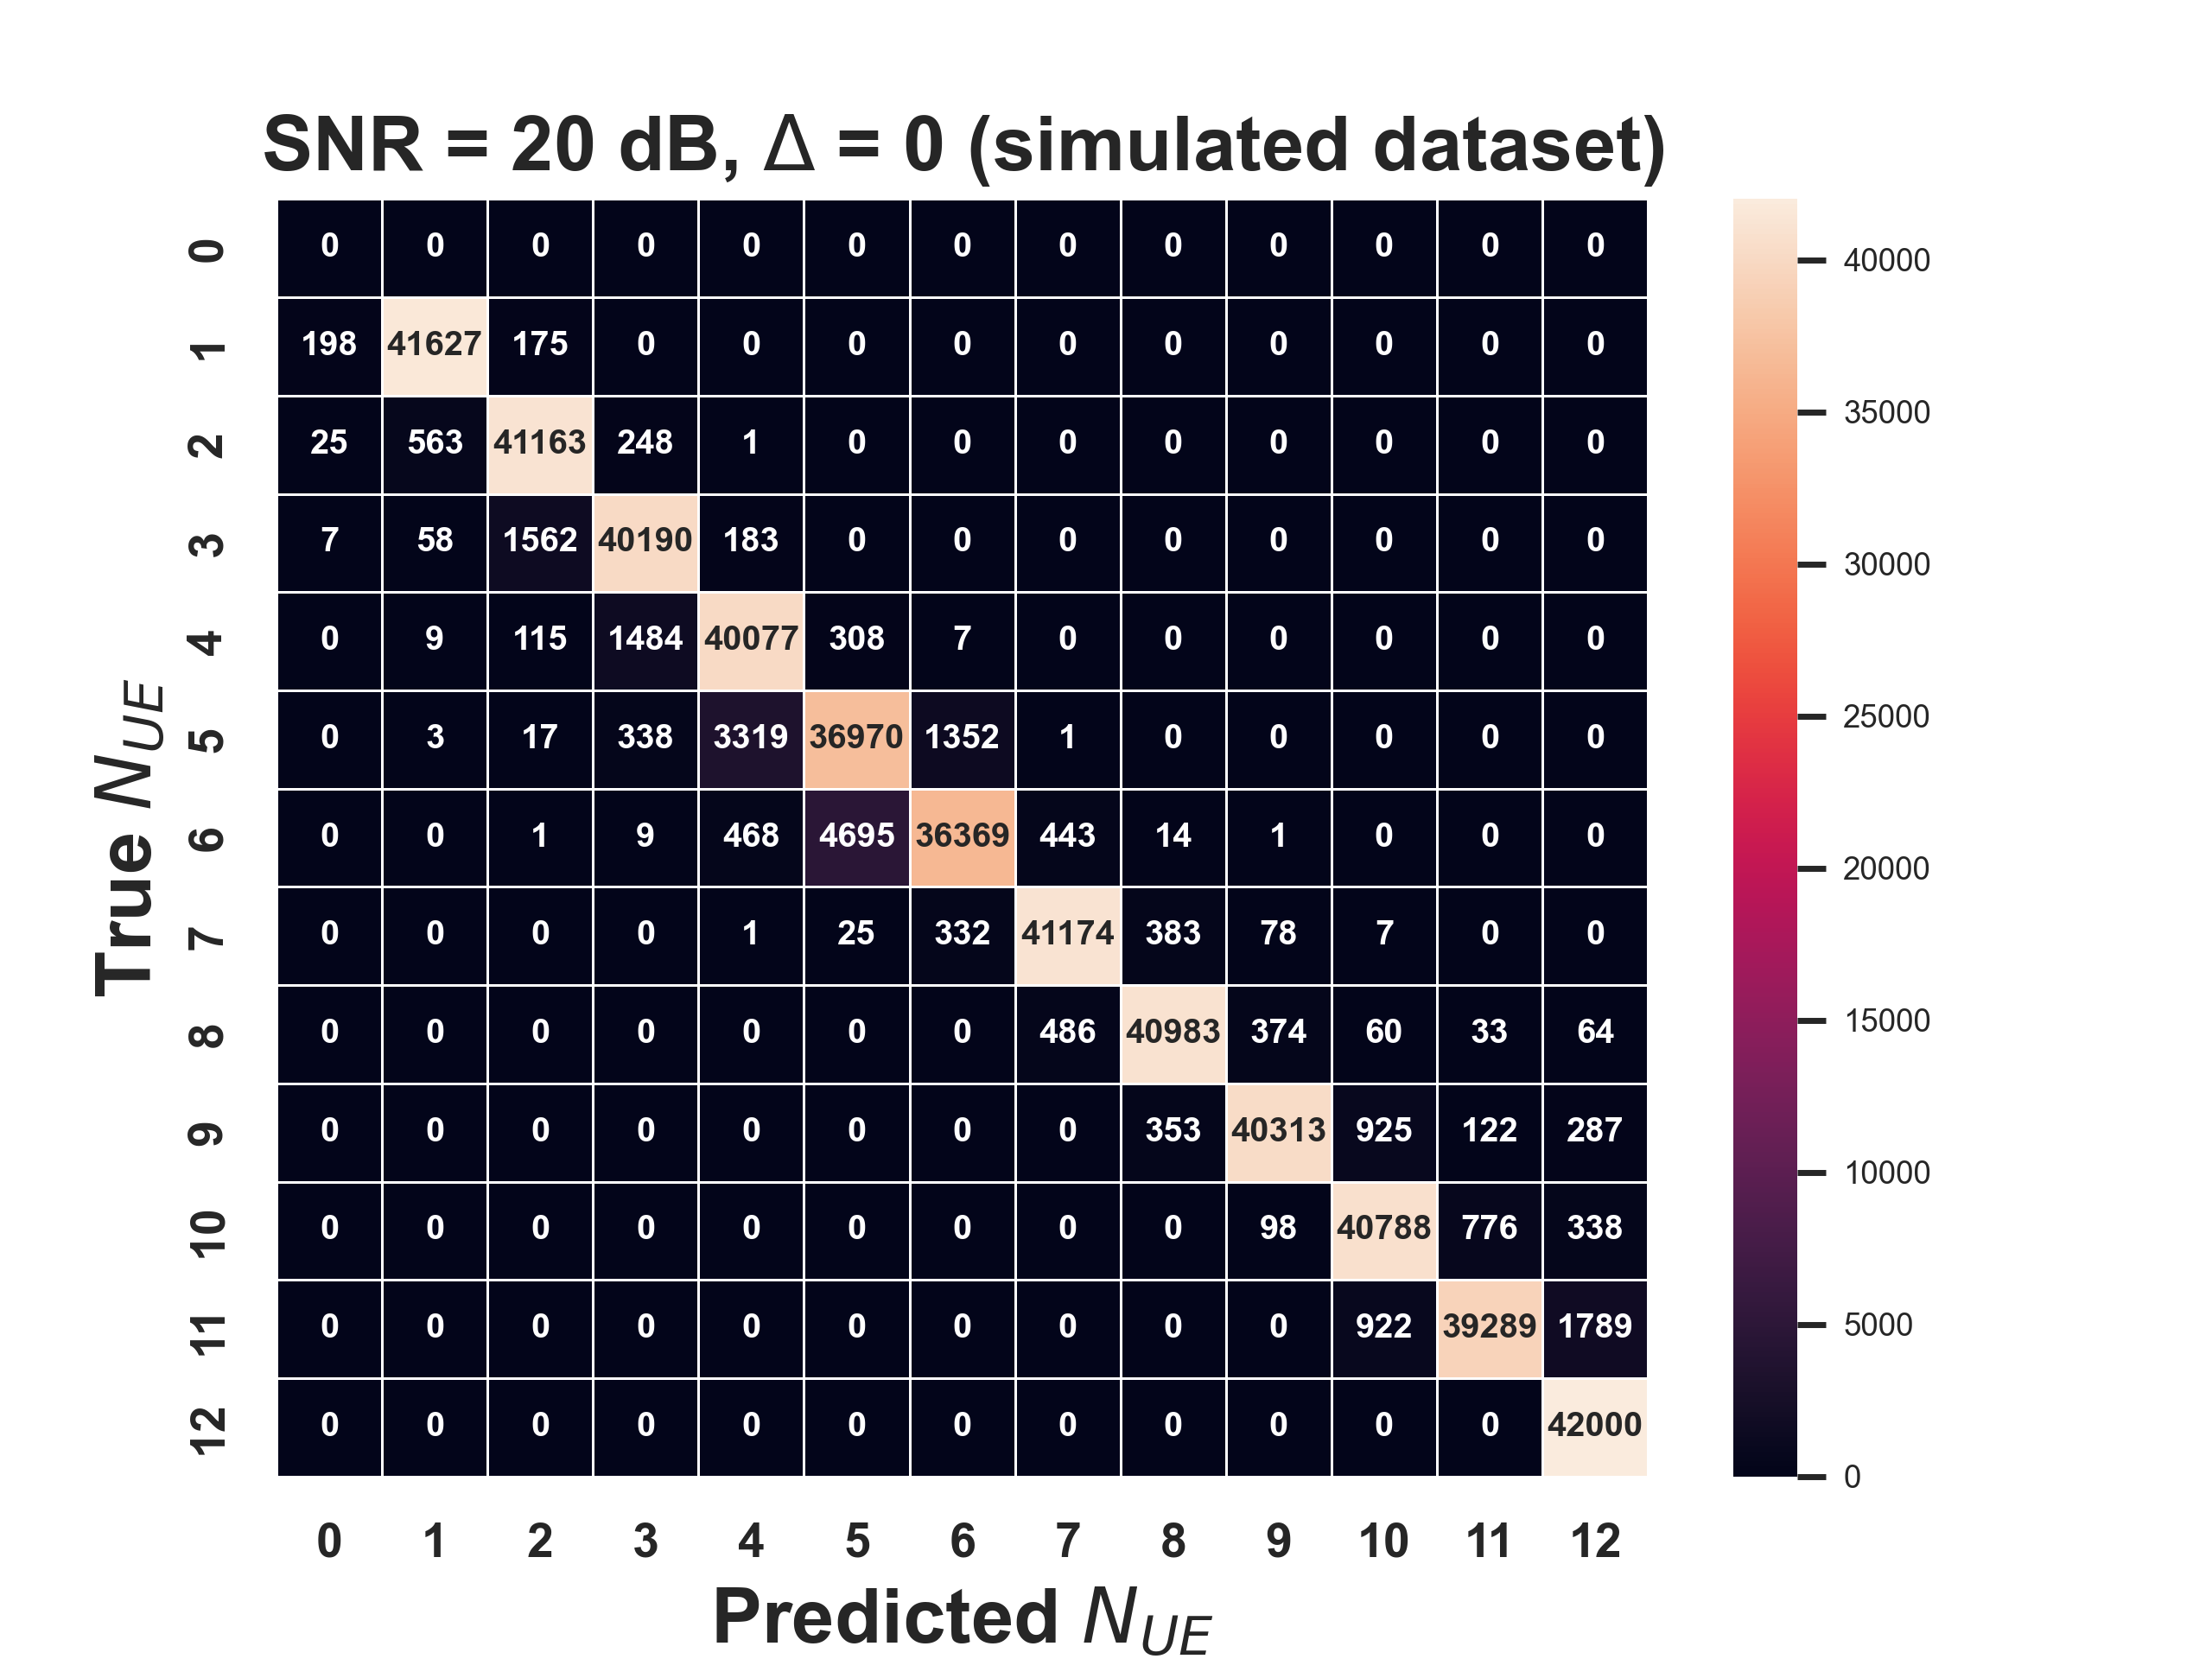
\includegraphics[width=\textwidth]{Figures/Conf_mtx_num_UEs_SNR_20_dB_Max_off_0_train_sim_test_sim.png}
         \caption{}
         \label{fig: cm_num_UE_snr_20_off_0_sim}
     \end{subfigure}
     \\
     \begin{subfigure}[b]{0.48\textwidth}
         \centering
         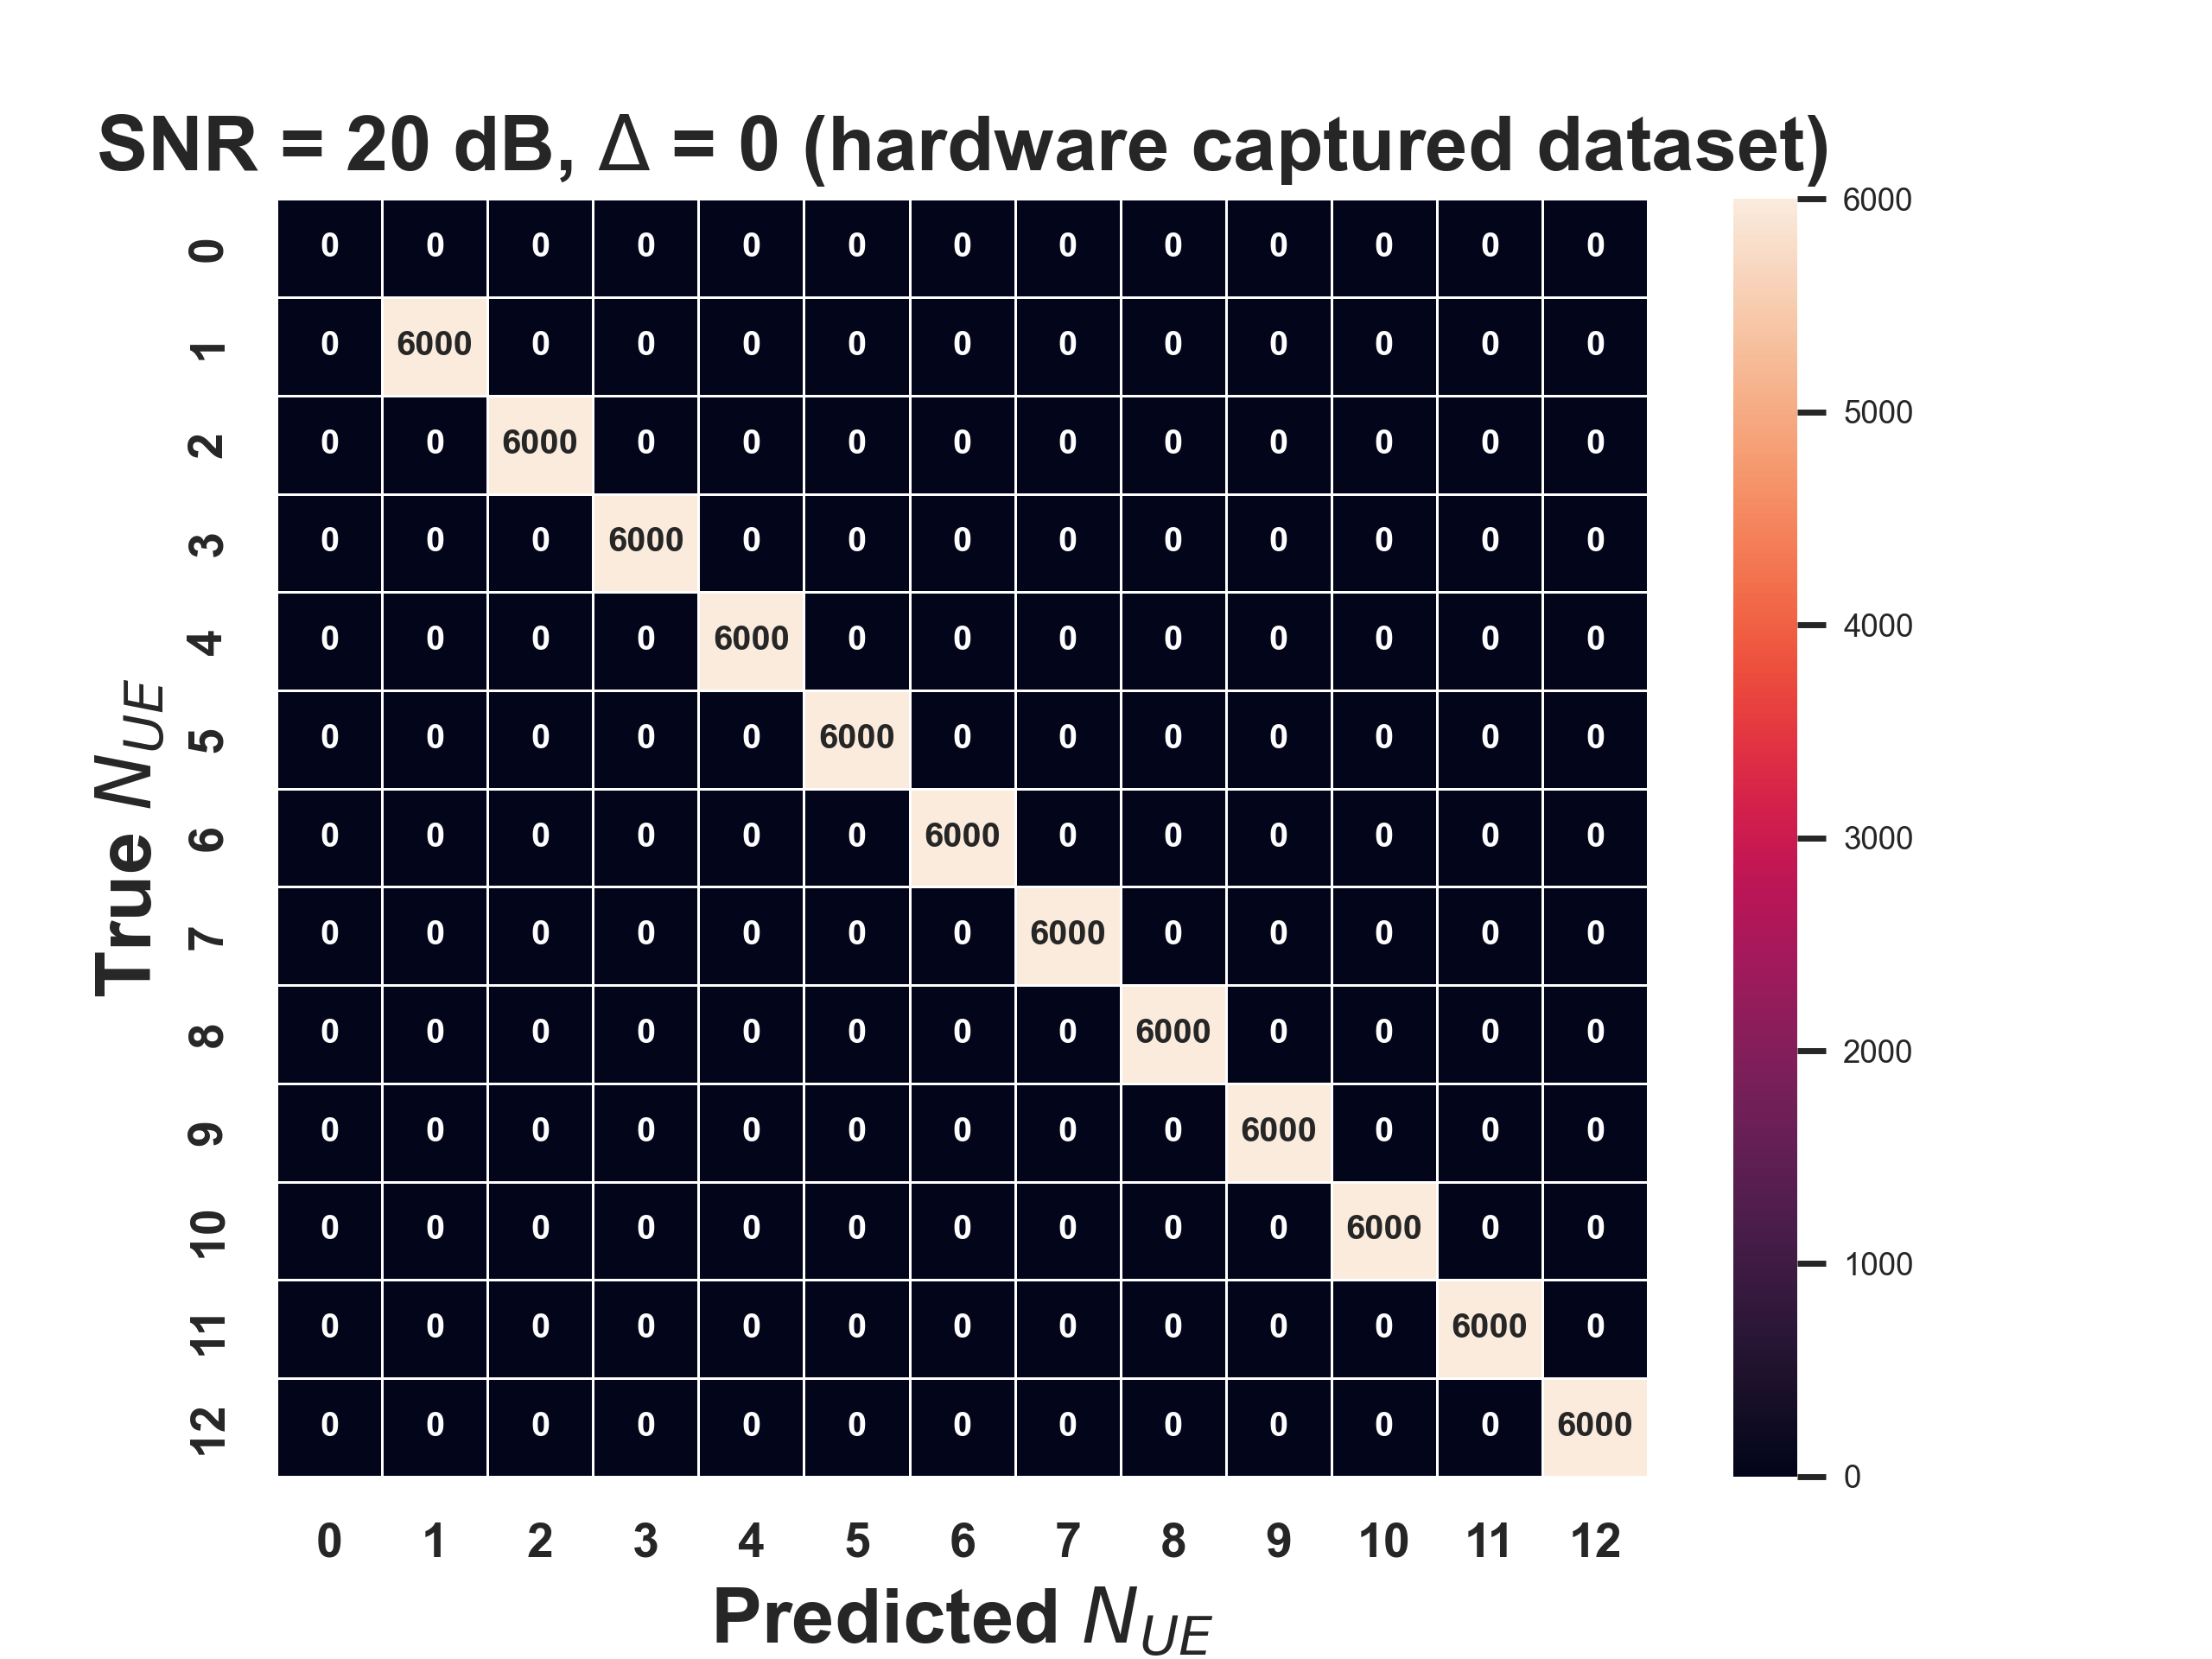
\includegraphics[width=\textwidth]{Figures/Conf_mtx_num_UEs_SNR_20_dB_Max_off_0_train_sim_test_hw.png}
         \caption{}
         \label{fig: cm_num_UE_snr_20_off_0_hw}
     \end{subfigure}
        \caption{Confusion matrix for the number of multiplexed UEs $N_{UE}$, at SNR = $20$ dB and $\Delta$ = $0$ for (a) simulated test dataset and (b) hardware captured test dataset.}
        \label{fig: cm_num_UE_snr_20_off_0}
\end{figure}

\begin{figure}[ht!]
    \captionsetup{justification=justified}
     \centering
     \begin{subfigure}[b]{0.48\textwidth}
         \centering
         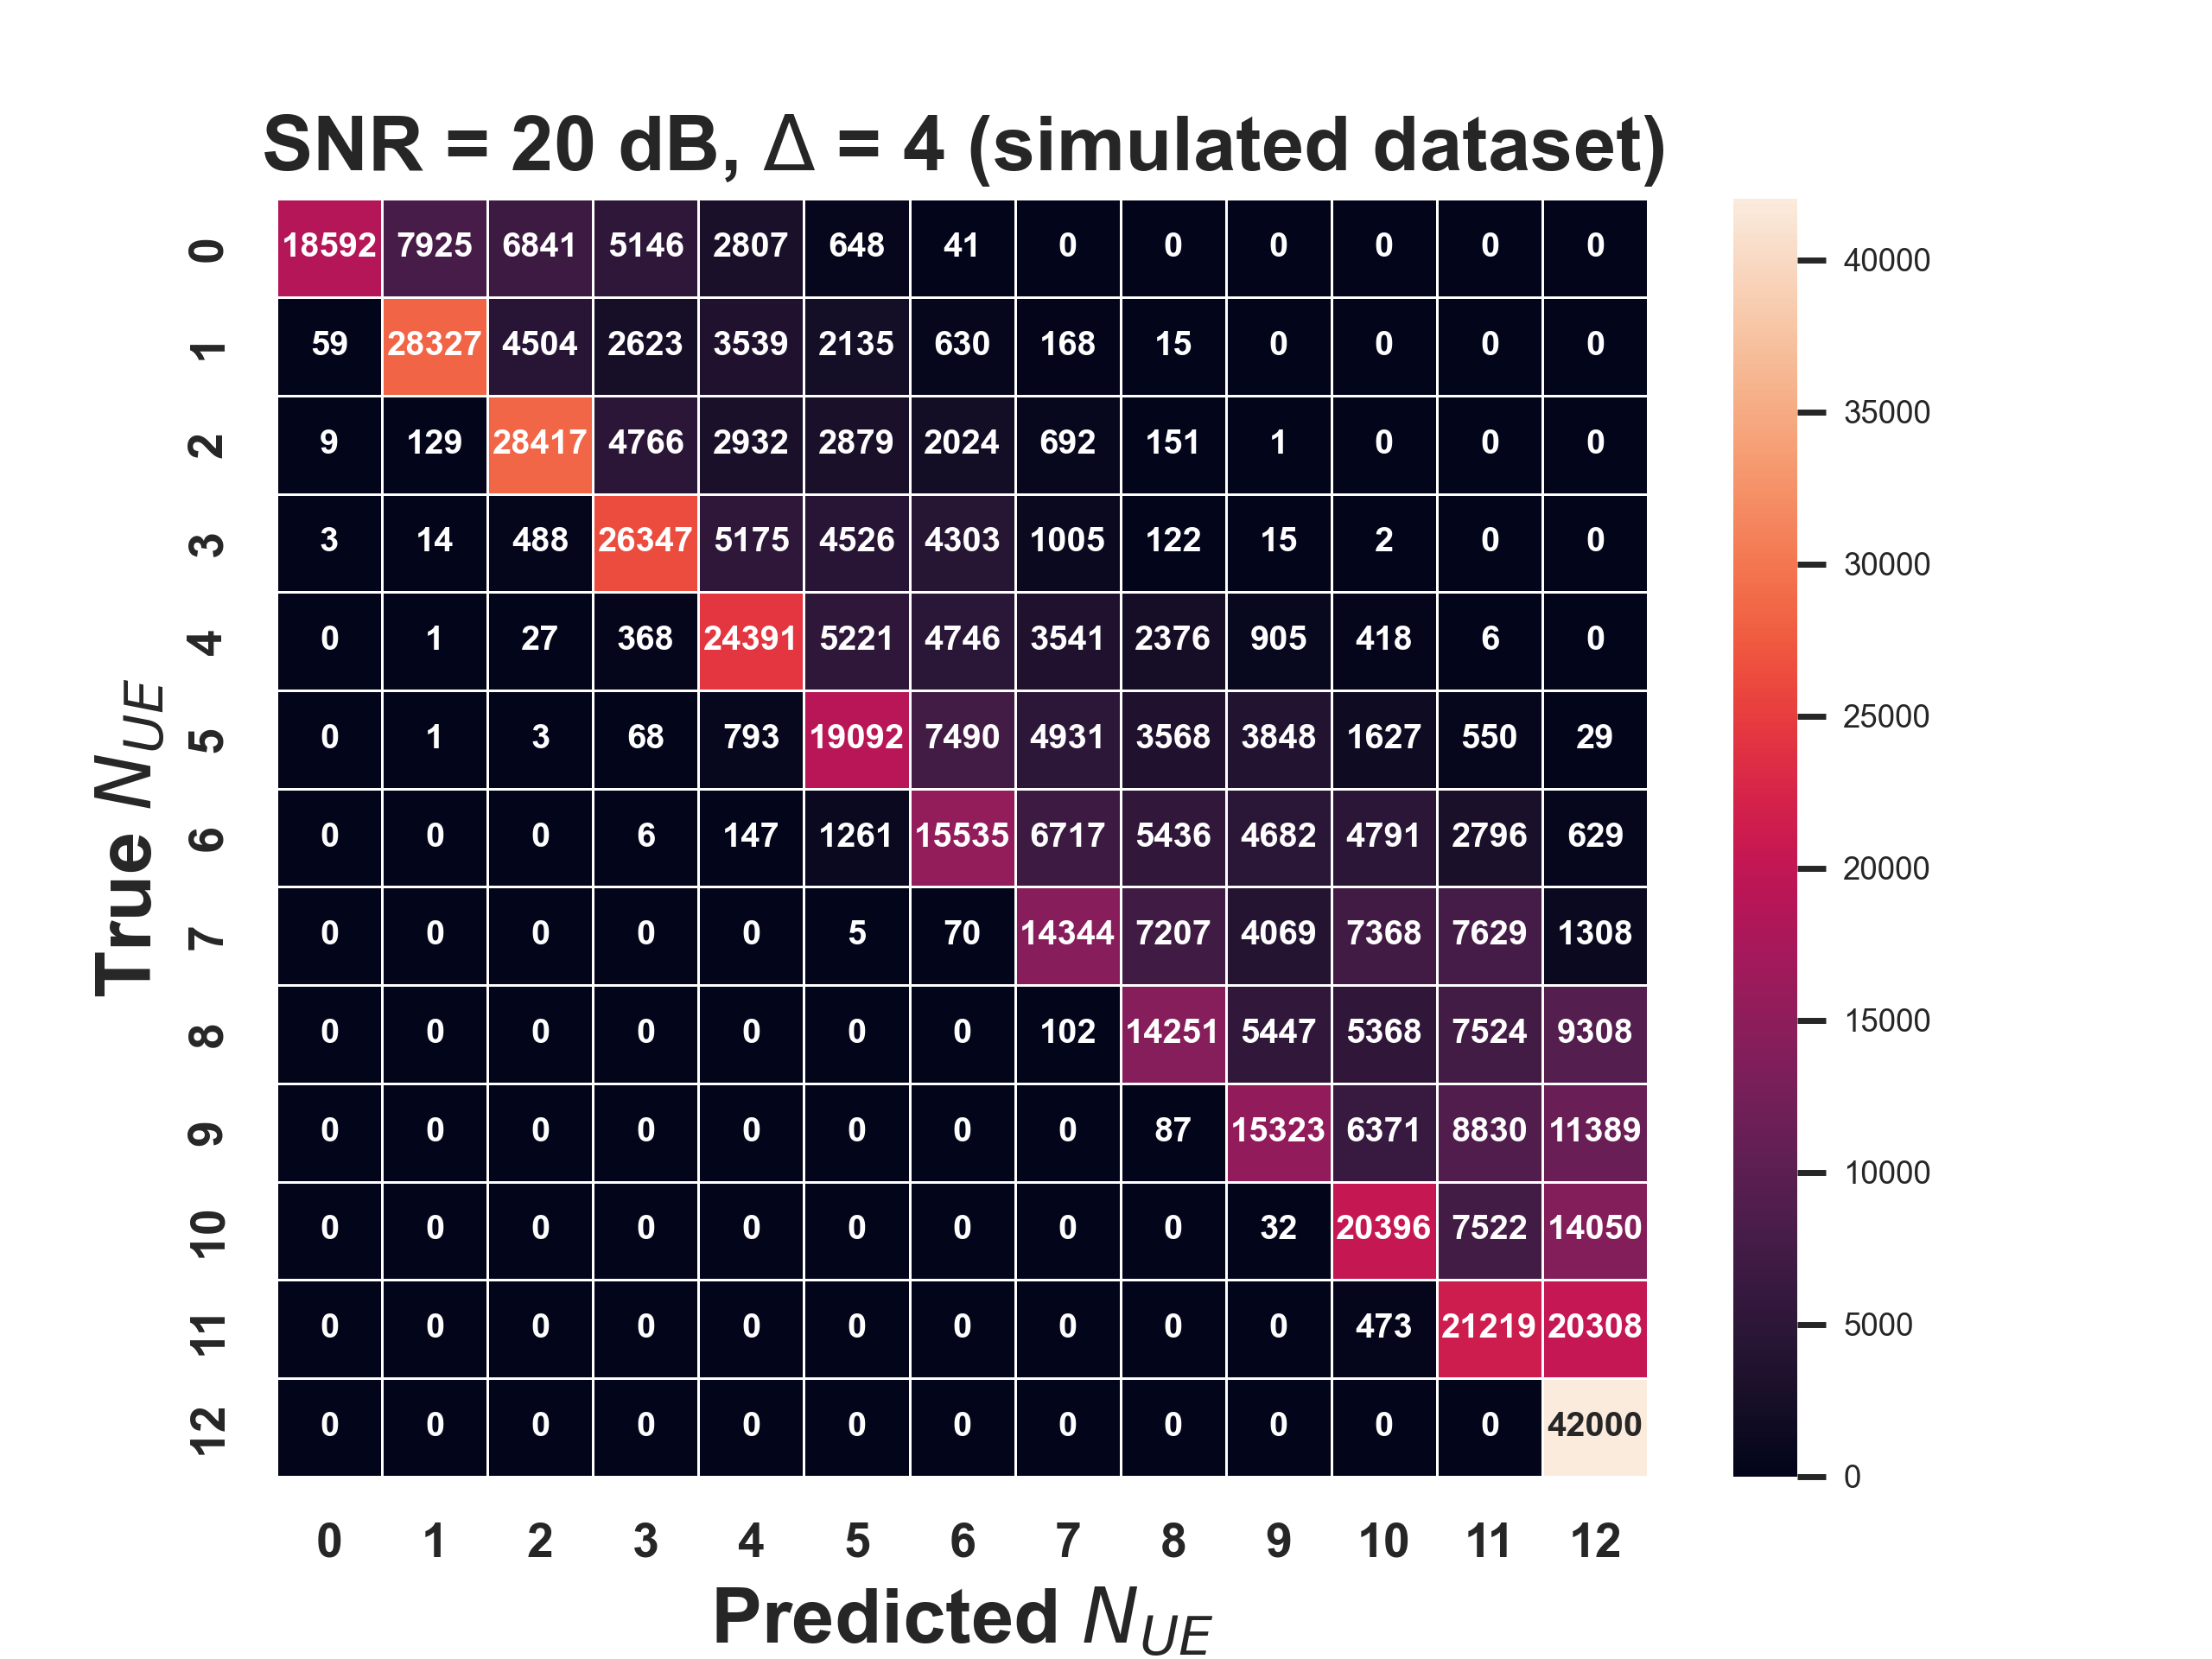
\includegraphics[width=\textwidth]{Figures/Conf_mtx_num_UEs_SNR_20_dB_Max_off_4_train_sim_test_sim.png}
         \caption{}
         \label{fig: cm_num_UE_snr_20_off_4_sim}
     \end{subfigure}
     \\
     \begin{subfigure}[b]{0.48\textwidth}
         \centering
         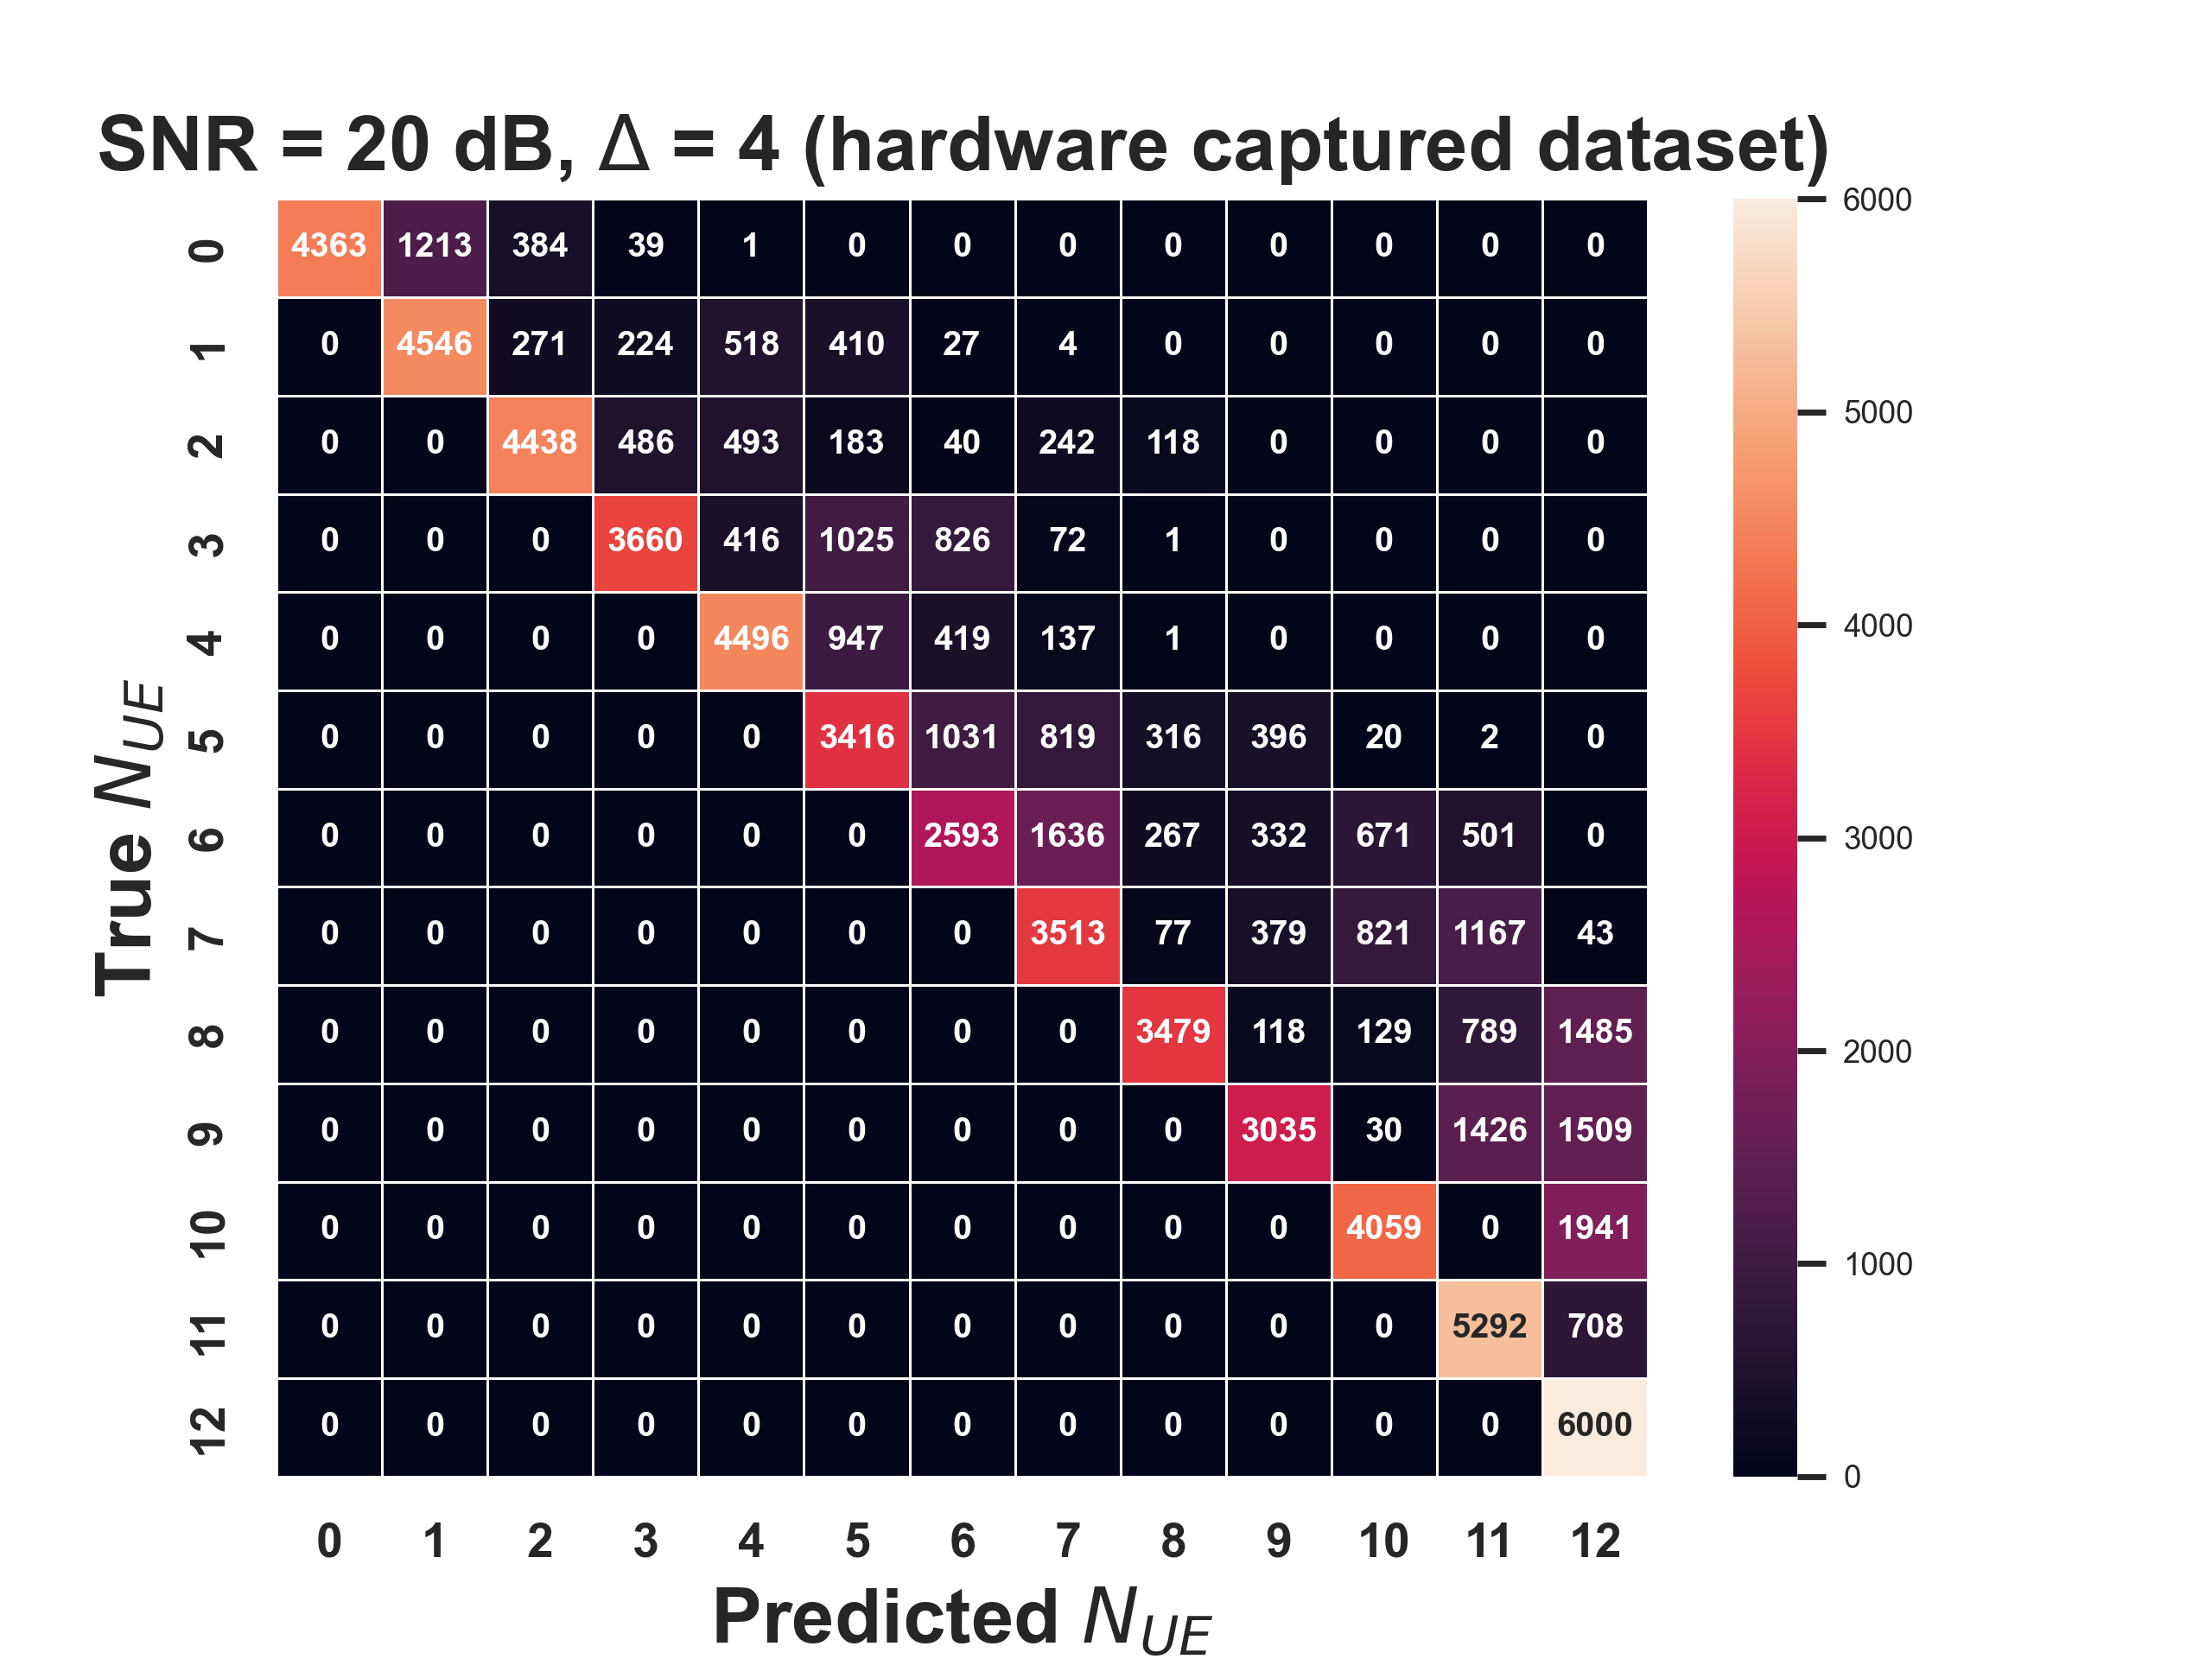
\includegraphics[width=\textwidth]{Figures/Conf_mtx_num_UEs_SNR_20_dB_Max_off_4_train_sim_test_hw.png}
         \caption{}
         \label{fig: cm_num_UE_snr_20_off_4_hw}
     \end{subfigure}
        \caption{Confusion matrix for the number of multiplexed UEs $N_{UE}$, at SNR = $20$ dB and $\Delta$ = $4$ for (a) simulated test dataset and (b) hardware captured test dataset.}
        \label{fig: cm_num_UE_snr_20_off_4}
\end{figure}

The column charts in Figure~\ref{fig: bar_alpha_SNR_snr_0_off_4} and Figure~\ref{fig: bar_alpha_SNR_snr_20_off_4} show the percentage of correct and incorrect predictions for the transmission of every $\alpha$ from 0 through 11. The result of the NN model's prediction for the scenario where a particular $\alpha$ has not been transmitted by any UE is also captured in the last column labeled $No\ Tx$. Correct prediction in the last column indicates that the model was able to correctly identify the non-transmission of a particular $\alpha$ value, and incorrect detection determines the instances where a particular $\alpha$ has not been transmitted but incorrectly predicted. 

From Figure~\ref{fig: bar_alpha_SNR_snr_0_off_4} and Figure~\ref{fig: bar_alpha_SNR_snr_20_off_4}, it is evident that the NN model is not biased towards any particular $\alpha$ and the cyclic shifts are correctly identified in the majority of instances.

% \begin{figure}[ht!]
%     \captionsetup{justification=justified}
%      \centering
%      \begin{subfigure}[b]{0.48\textwidth}
%          \centering
%          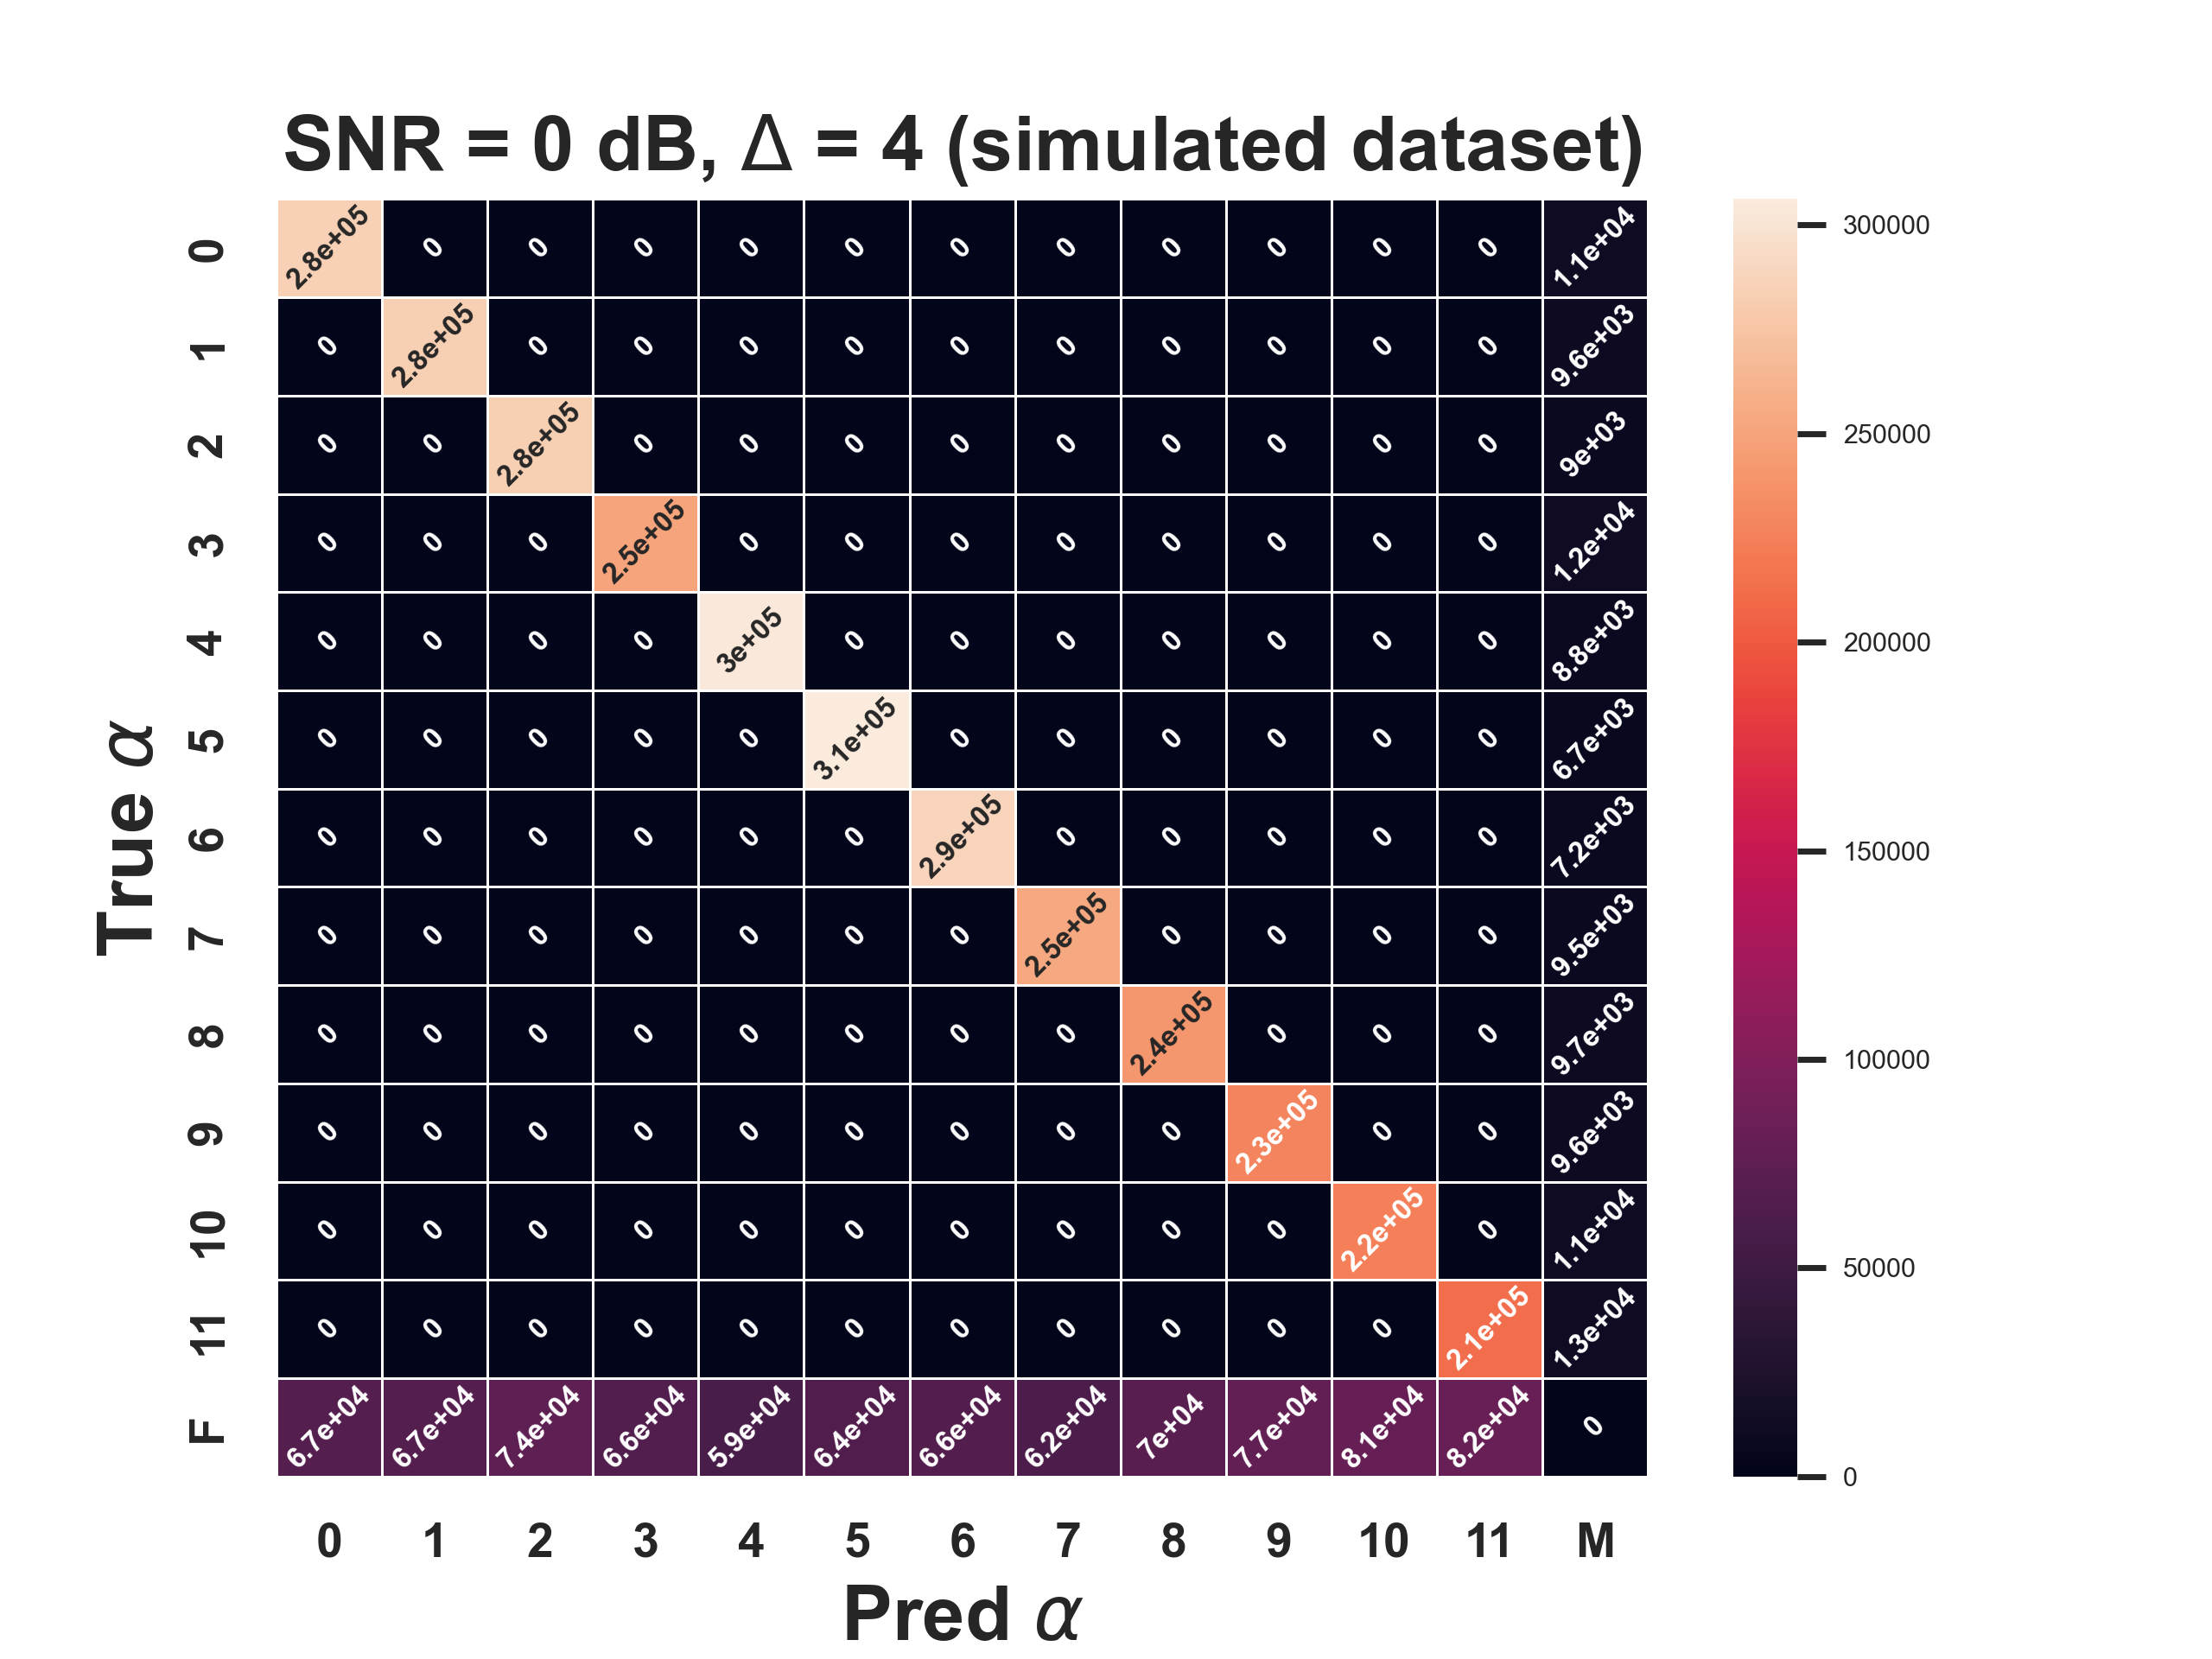
\includegraphics[width=\textwidth]{Figures/Conf_mtx_alpha_SNR_SNR_0_dB_Max_off_4_train_sim_test_sim.png}
%          \caption{}
%          \label{fig: cm_alpha_SNR_snr_0_off_4_sim}
%      \end{subfigure}
%      \\
%      \begin{subfigure}[b]{0.48\textwidth}
%          \centering
%          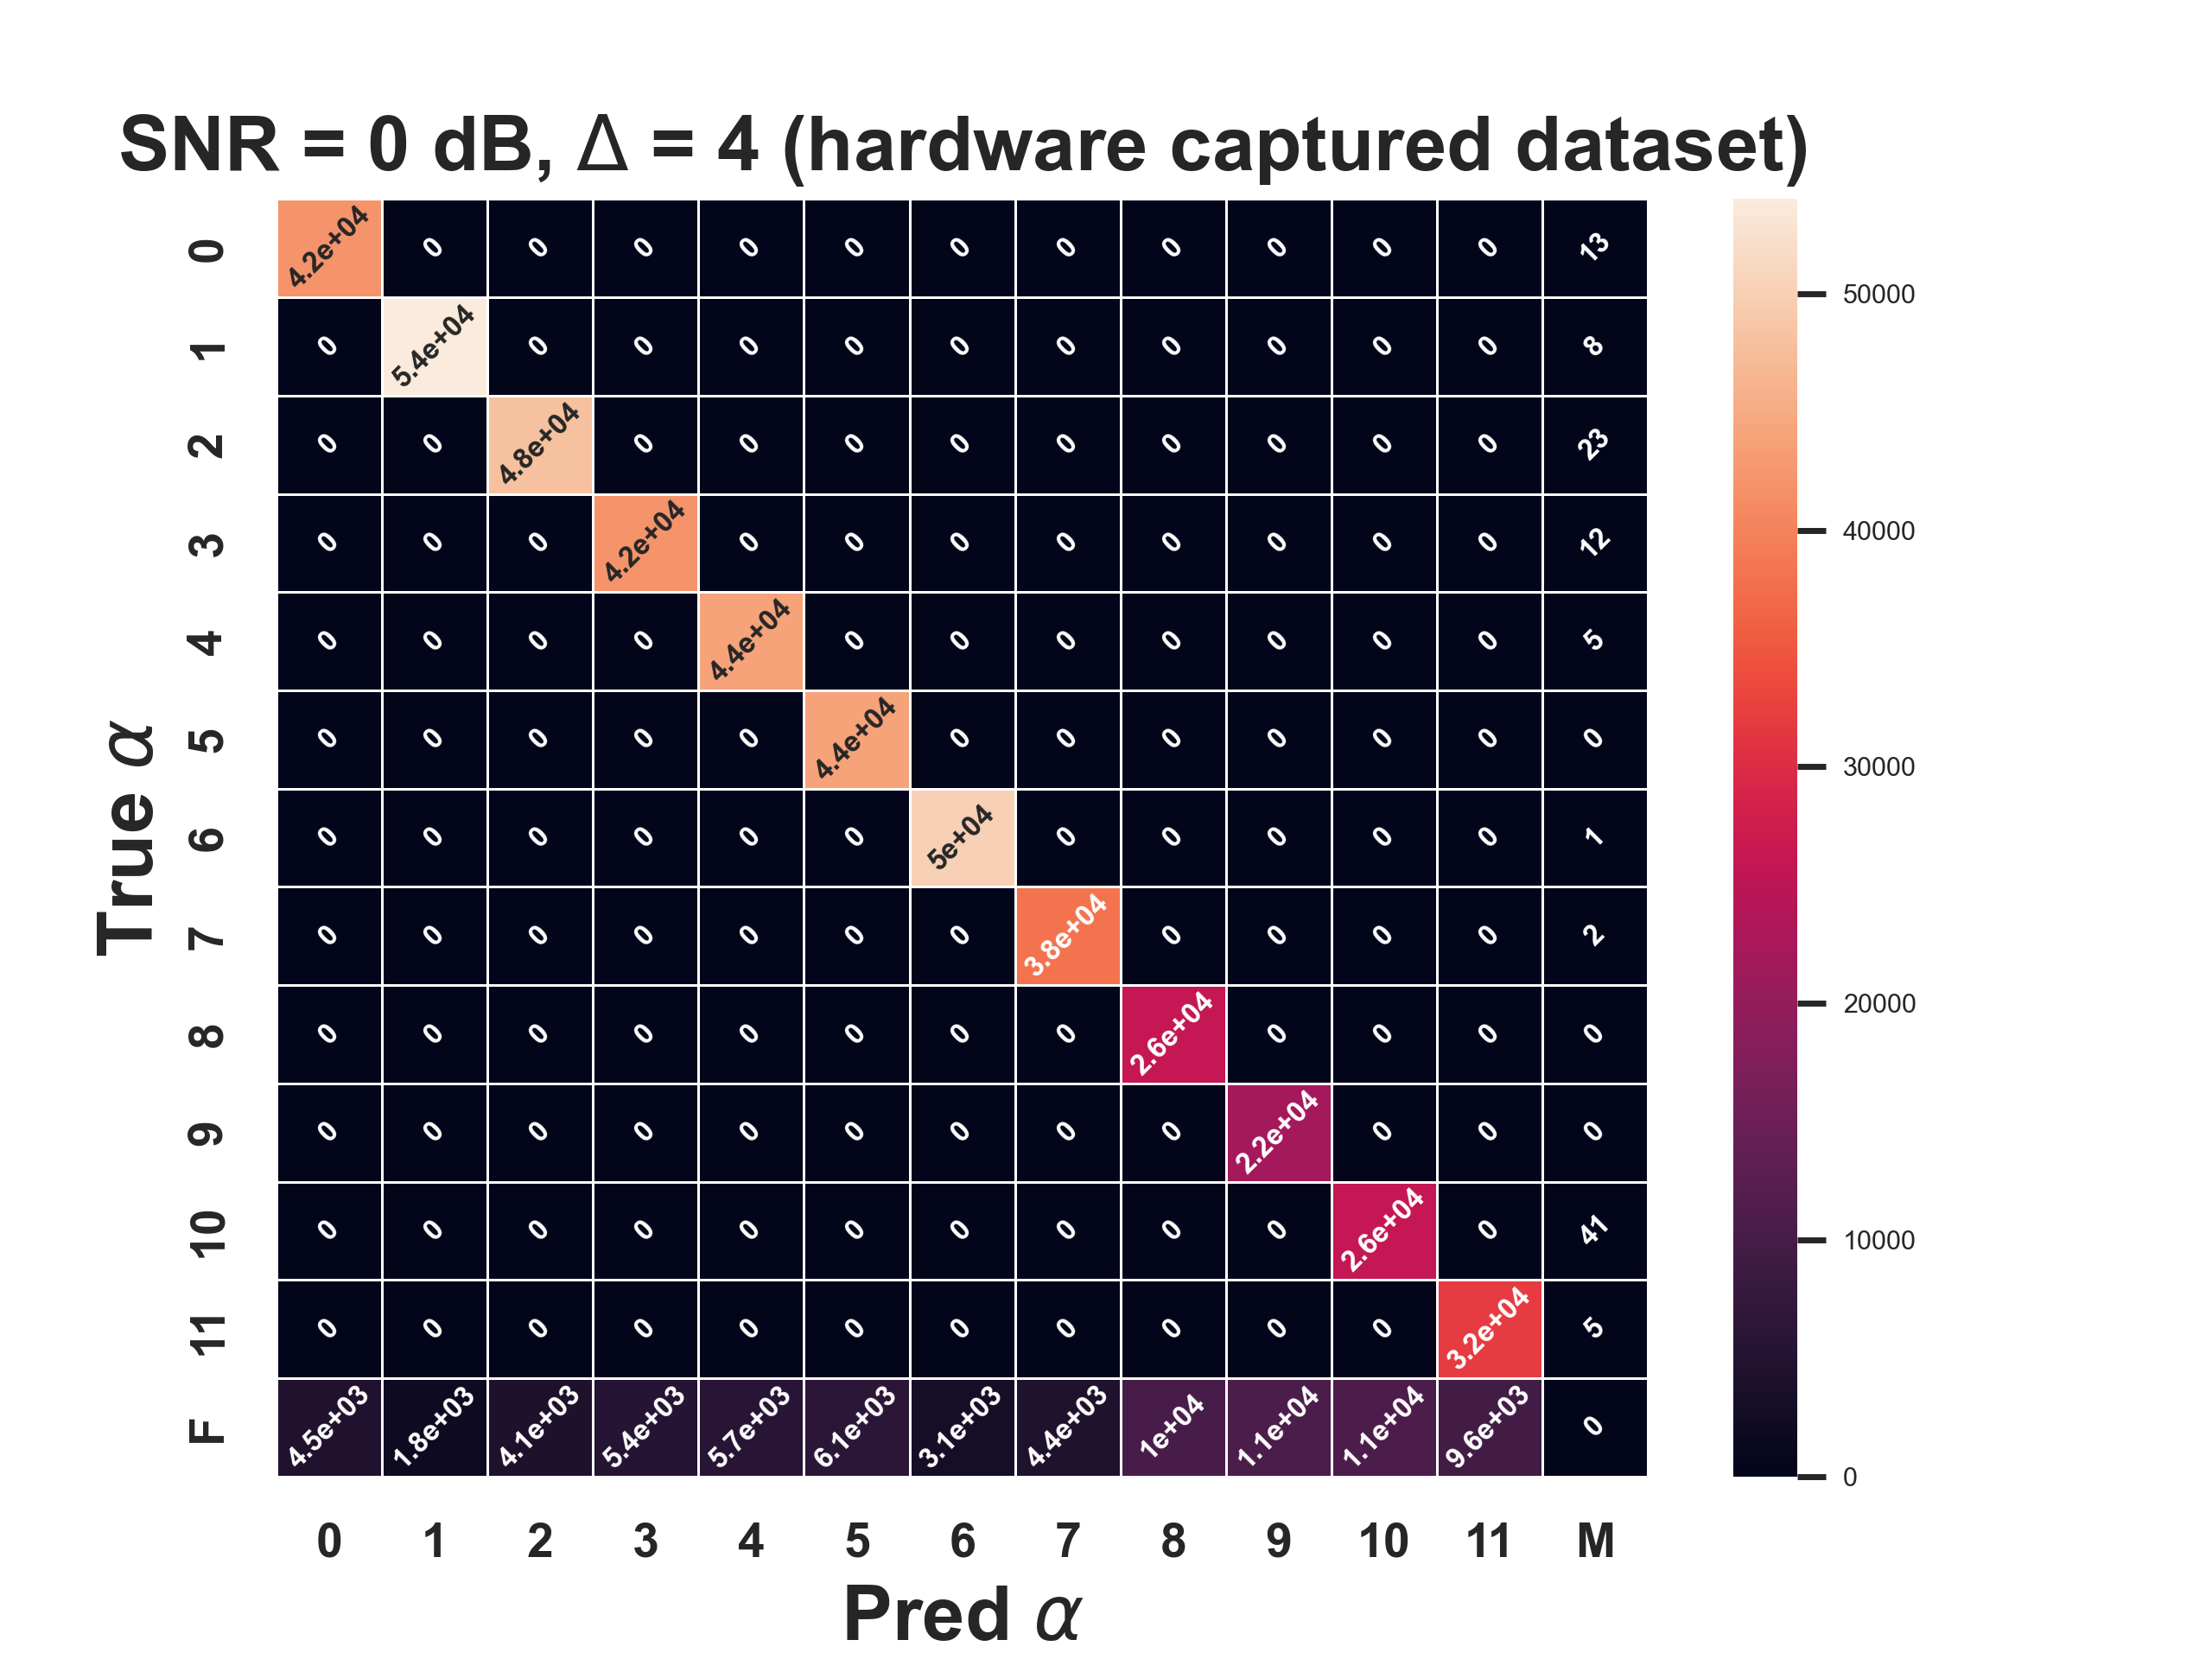
\includegraphics[width=\textwidth]{Figures/Conf_mtx_alpha_SNR_SNR_0_dB_Max_off_4_train_sim_test_hw.png}
%          \caption{}
%          \label{fig: cm_alpha_SNR_snr_0_off_4_hw}
%      \end{subfigure}
%         \caption{Confusion matrix for the cyclic shift $\alpha$ at SNR = $0$ dB, $\Delta$ = $4$, and with $N_{UE} = \{0, 1, 2, \dots, 12\}$ for (a) simulated test dataset and (b) hardware captured dataset}
%         \label{fig: cm_alpha_SNR_snr_0_off_4}
% \end{figure}

\begin{figure}[ht!]
    \captionsetup{justification=justified}
     \centering
     \begin{subfigure}[b]{0.48\textwidth}
         \centering
         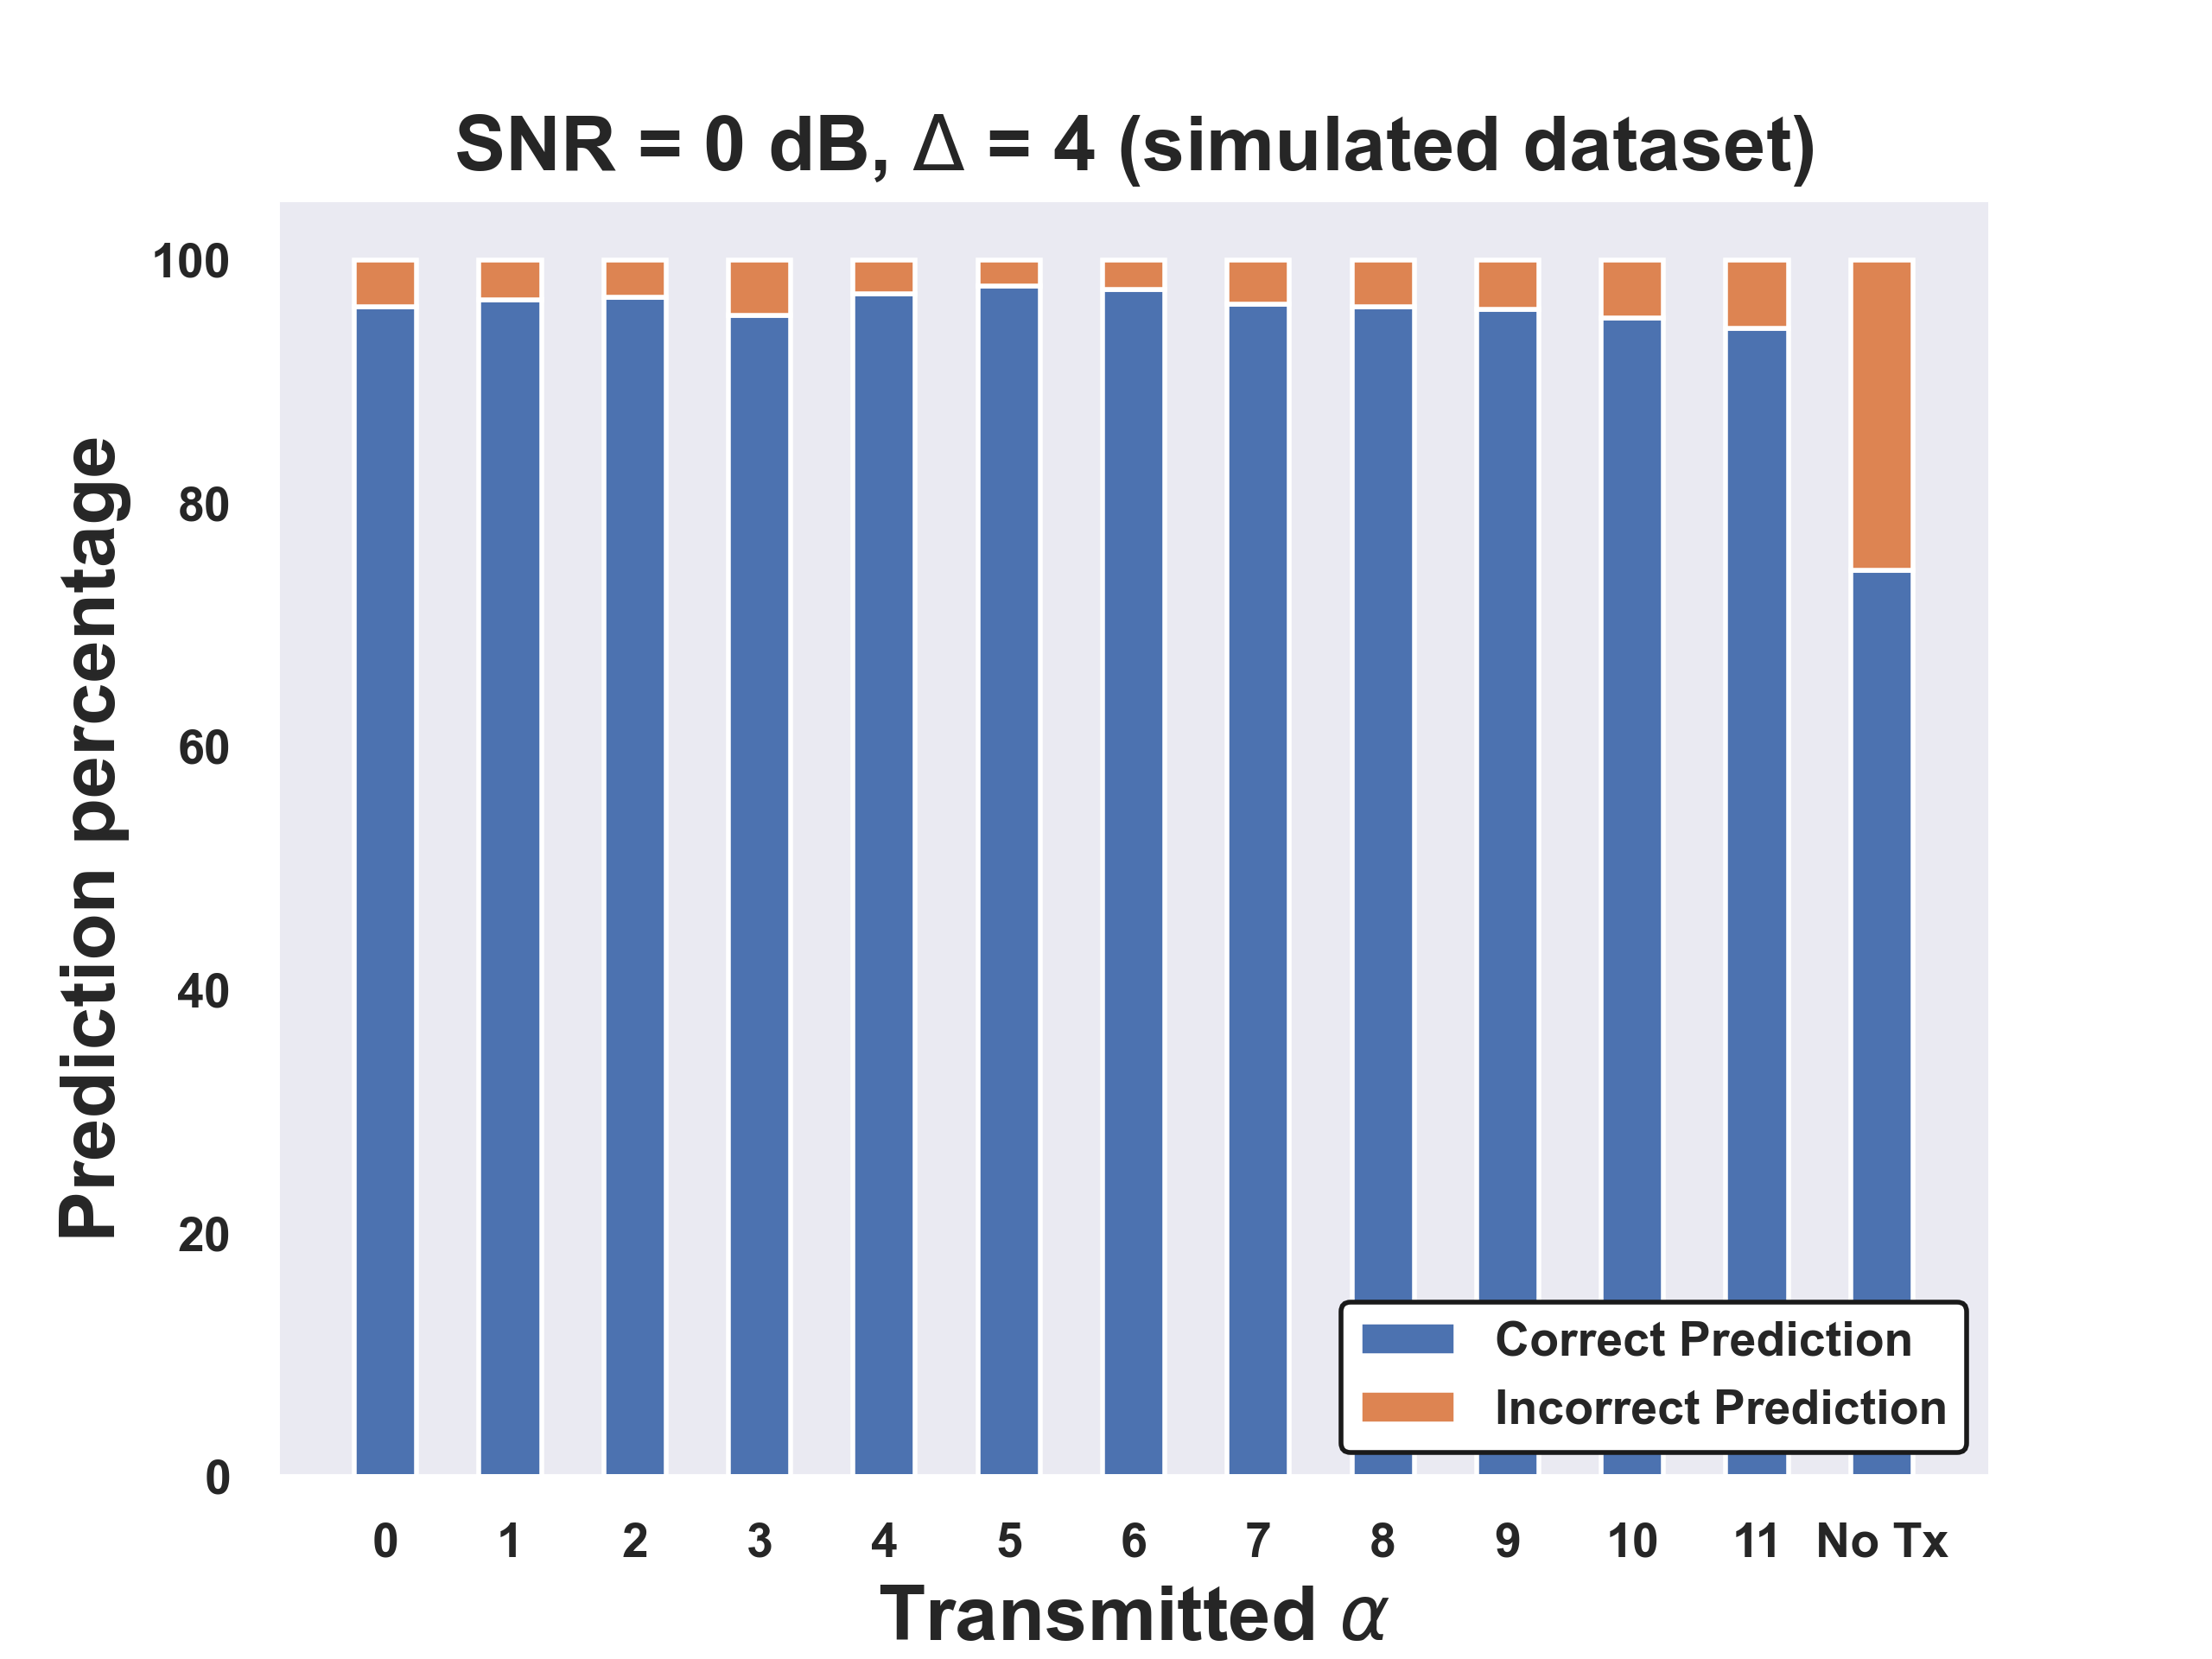
\includegraphics[width=\textwidth]{Figures/Bar_alpha_SNR_SNR_0_dB_Max_off_4_train_sim_test_sim.png}
         \caption{}
         \label{fig: bar_alpha_SNR_snr_0_off_4_sim}
     \end{subfigure}
     \\
     \begin{subfigure}[b]{0.48\textwidth}
         \centering
         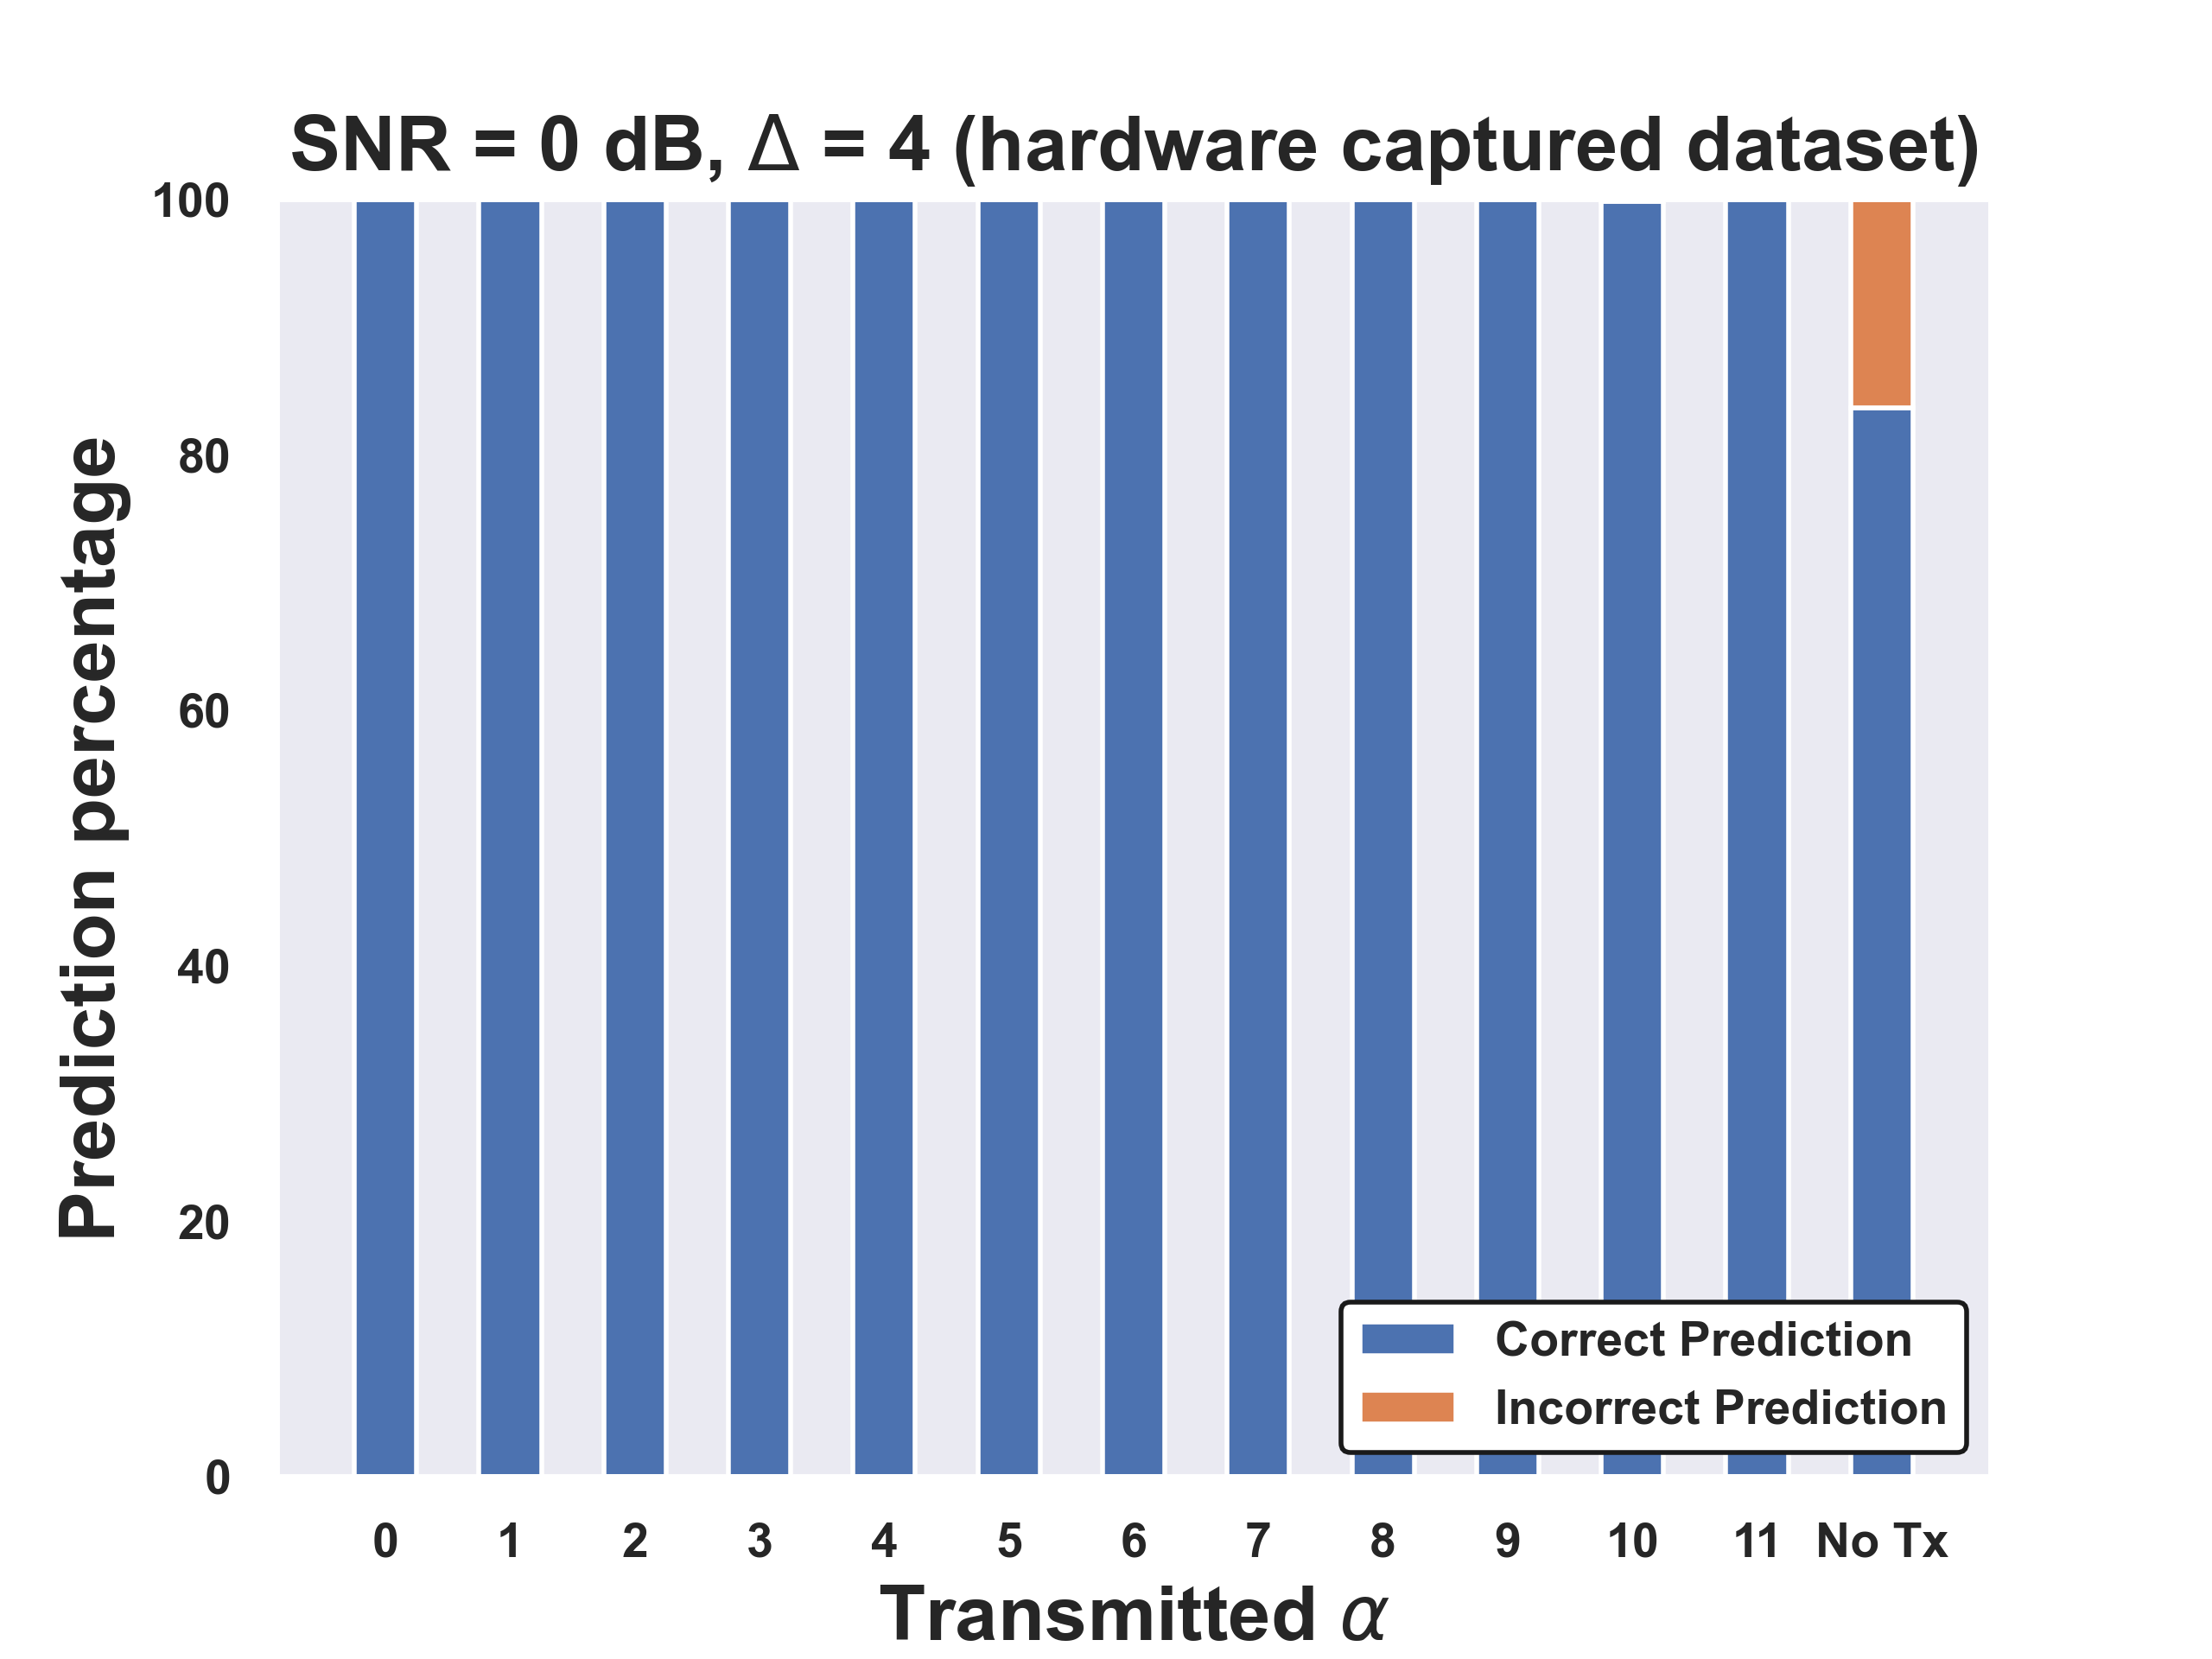
\includegraphics[width=\textwidth]{Figures/Bar_alpha_SNR_SNR_0_dB_Max_off_4_train_sim_test_hw.png}
         \caption{}
         \label{fig: bar_alpha_SNR_snr_0_off_4_hw}
     \end{subfigure}
        \caption{Bar graph for the cyclic shift $\alpha$ at SNR = $0$ dB, $\Delta$ = $4$, and with $N_{UE} = \{0, 1, 2, \dots, 12\}$ for (a) simulated test dataset and (b) hardware captured dataset.}
        \label{fig: bar_alpha_SNR_snr_0_off_4}
\end{figure}

\begin{figure}[ht!]
    \captionsetup{justification=justified}
     \centering
     \begin{subfigure}[b]{0.48\textwidth}
         \centering
         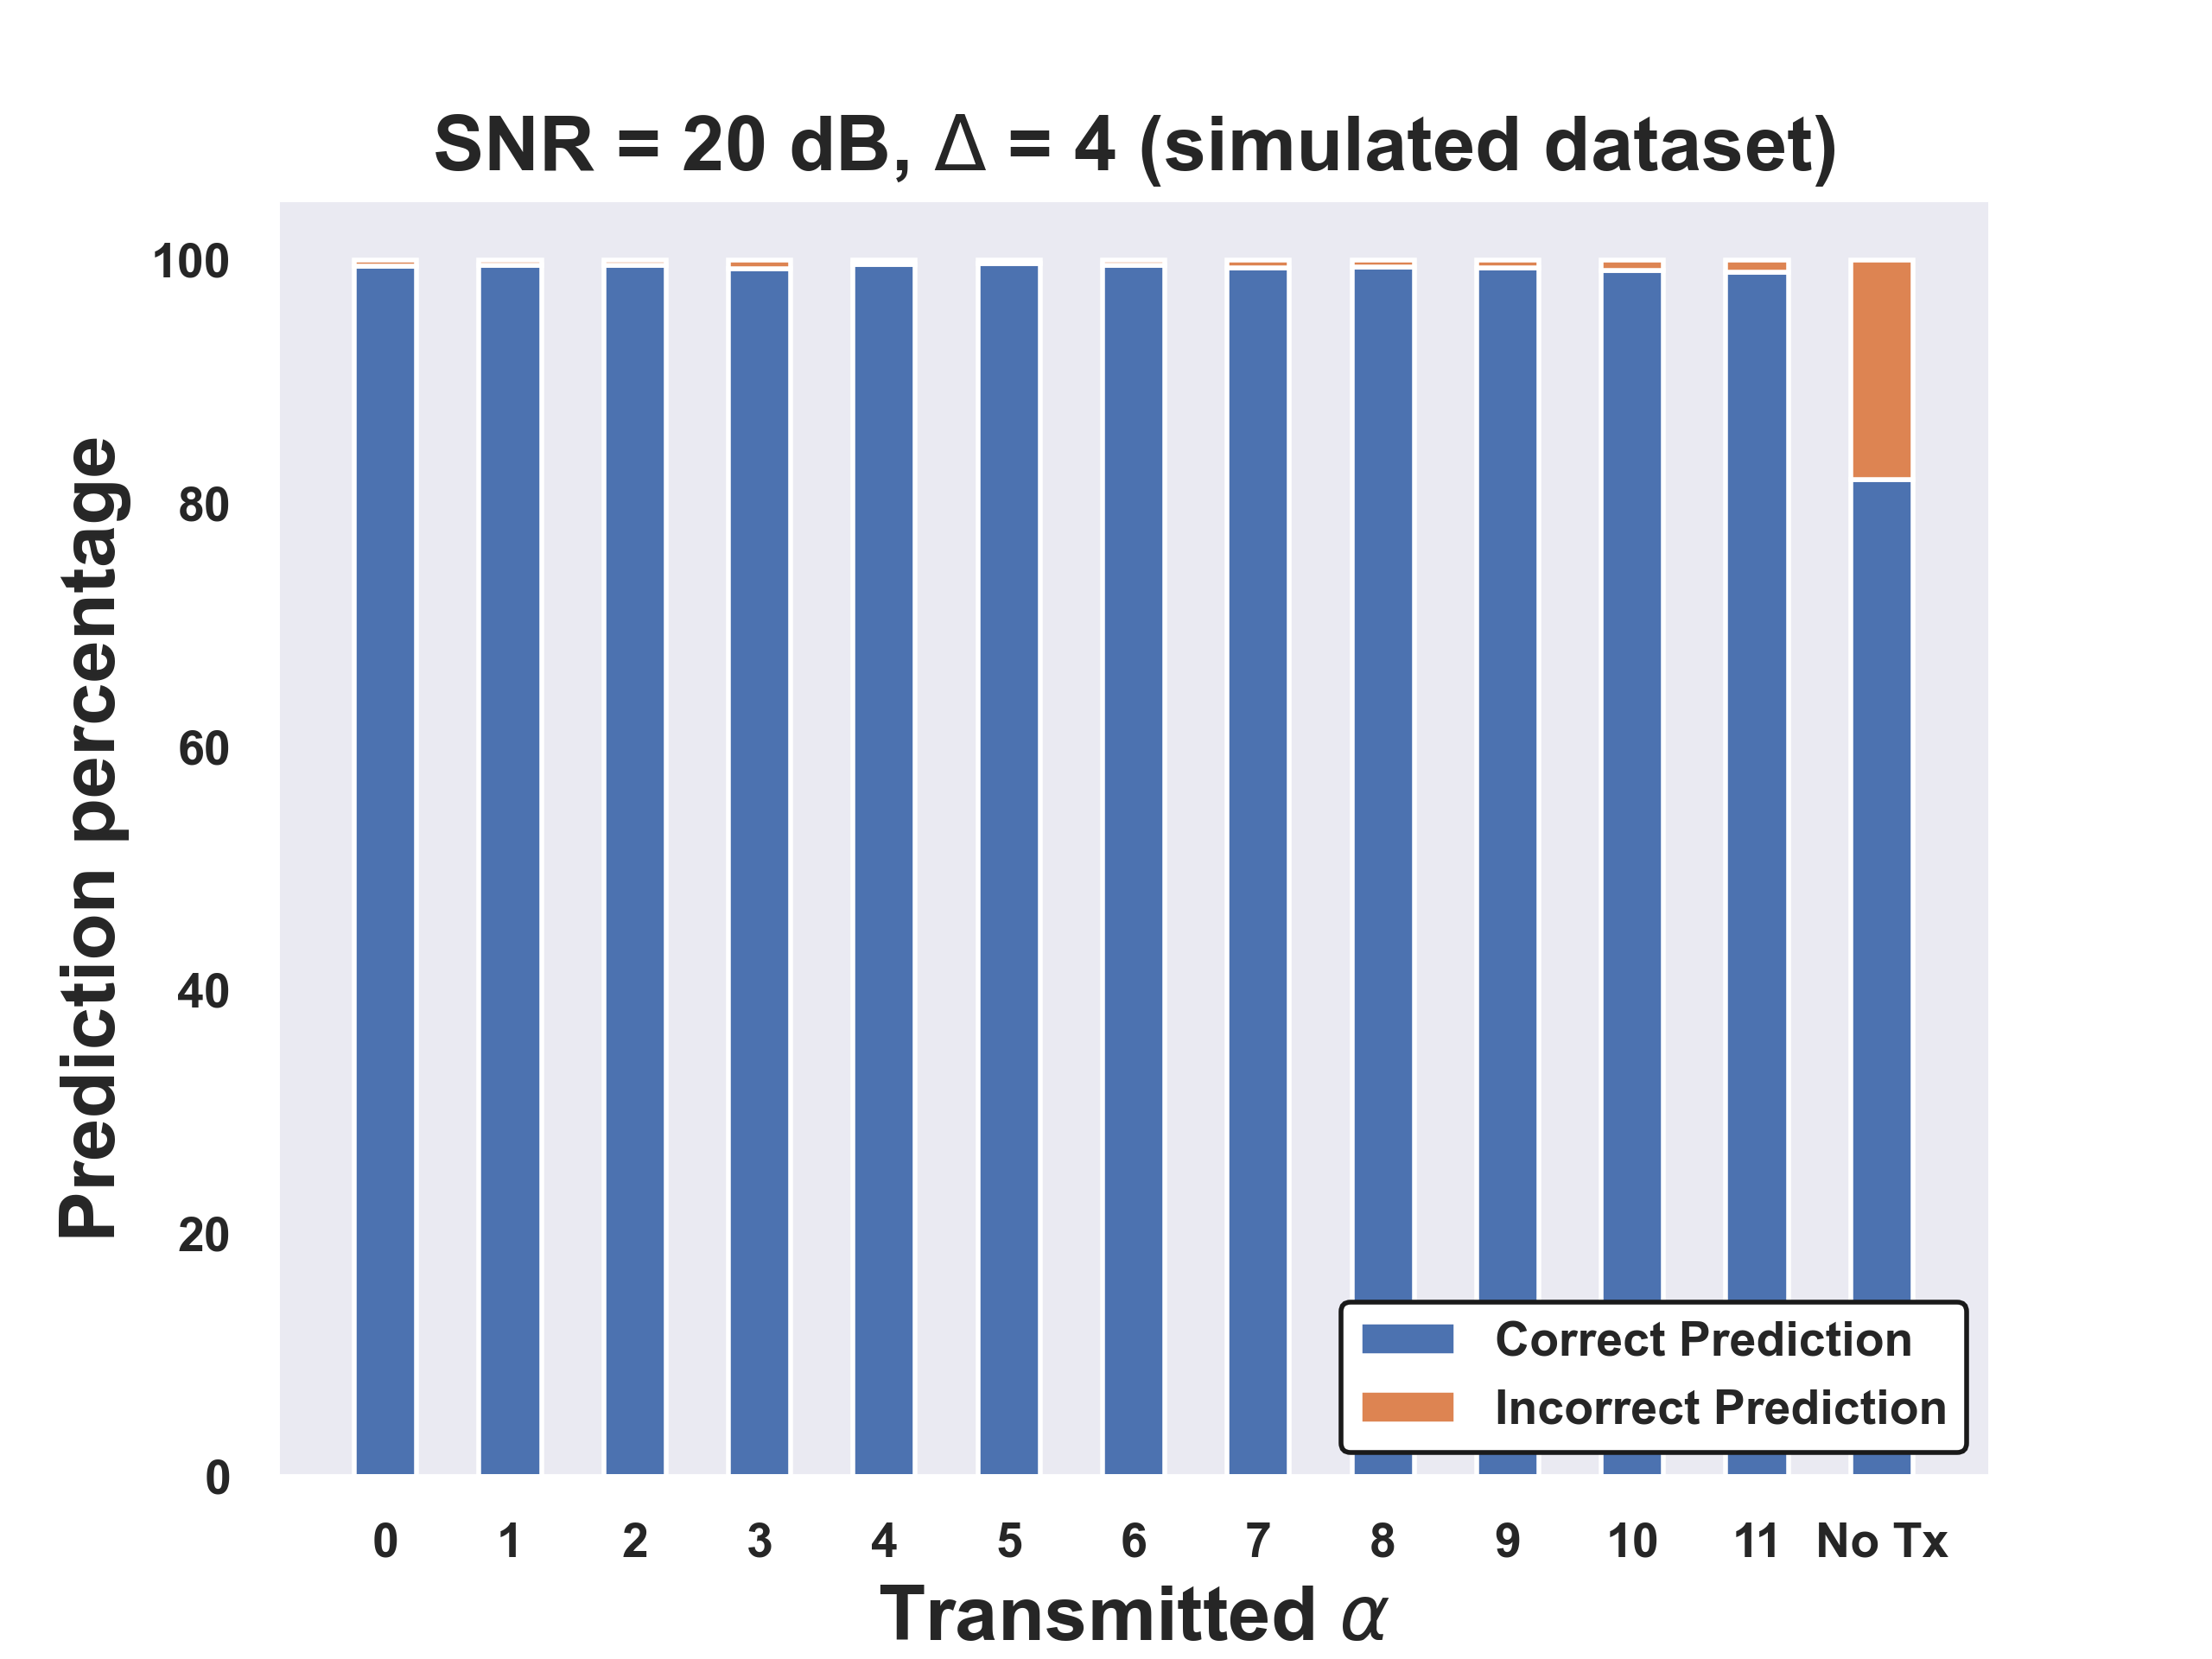
\includegraphics[width=\textwidth]{Figures/Bar_alpha_SNR_SNR_20_dB_Max_off_4_train_sim_test_sim.png}
         \caption{}
         \label{fig: bar_alpha_SNR_snr_20_off_4_sim}
     \end{subfigure}
     \\
     \begin{subfigure}[b]{0.48\textwidth}
         \centering
         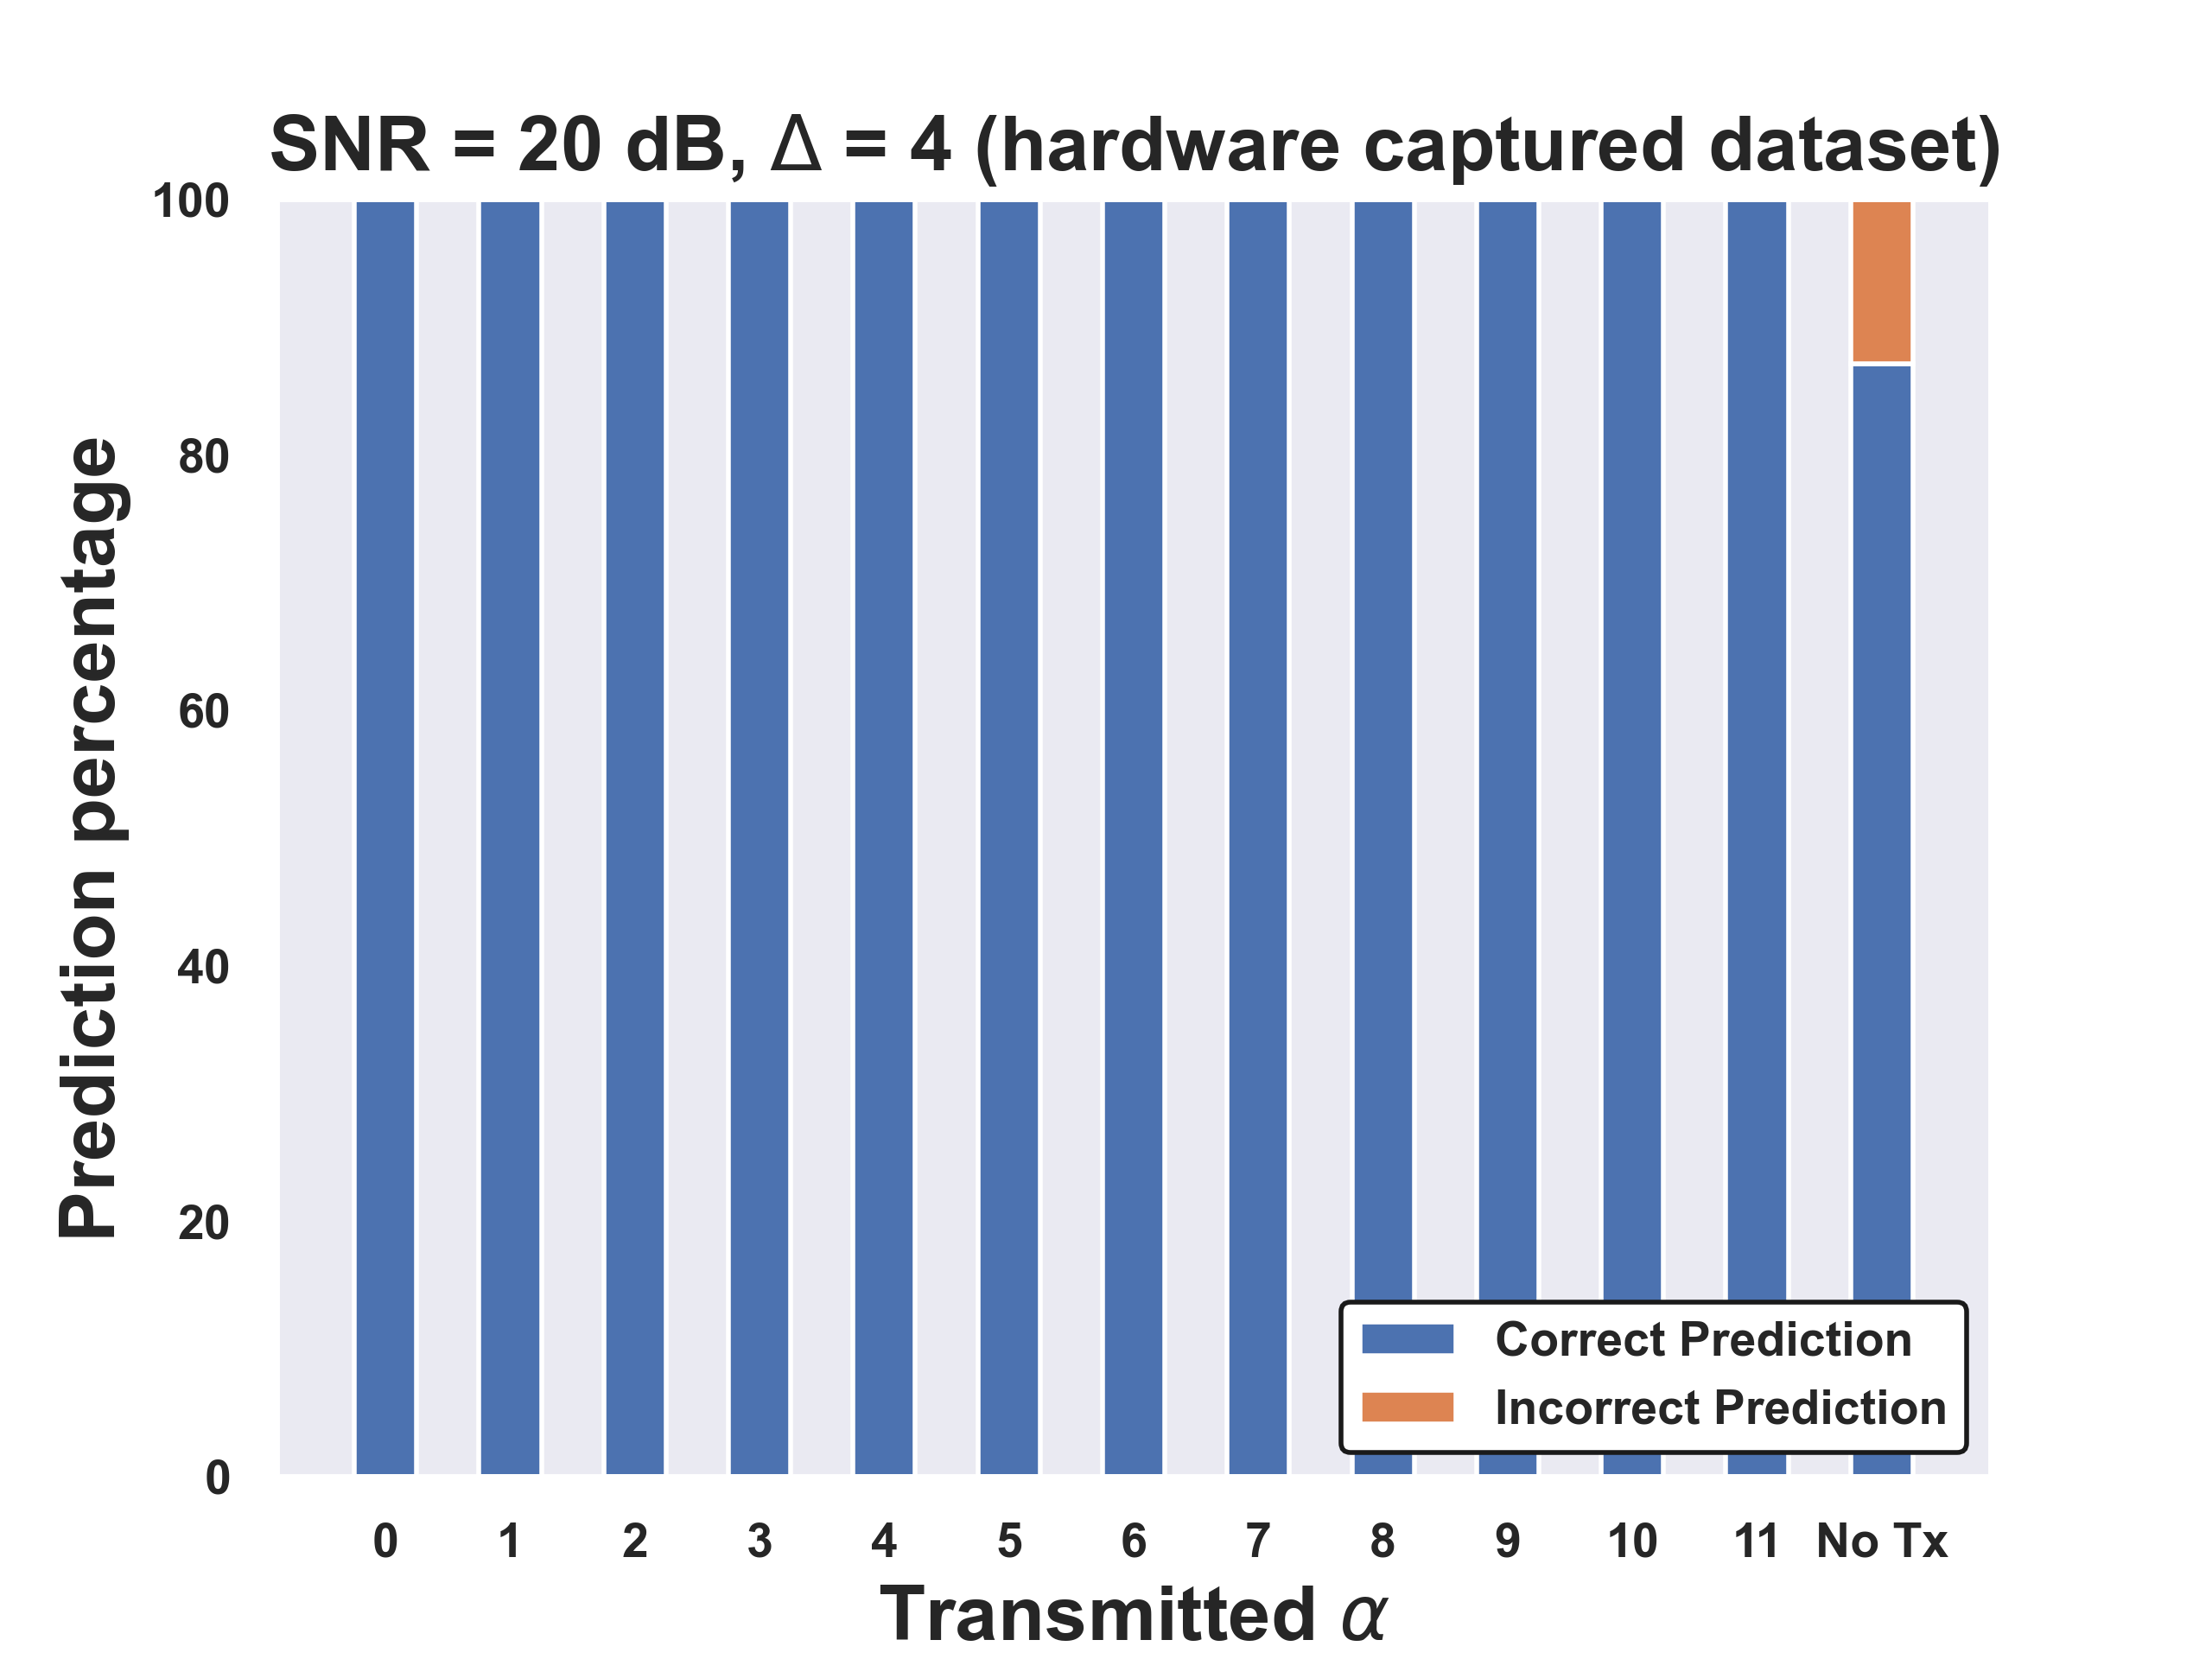
\includegraphics[width=\textwidth]{Figures/Bar_alpha_SNR_SNR_20_dB_Max_off_4_train_sim_test_hw.png}
         \caption{}
         \label{fig: bar_alpha_SNR_snr_20_off_4_hw}
     \end{subfigure}
        \caption{Bar graph for the cyclic shift $\alpha$ at SNR = $20$ dB, $\Delta$ = $4$, and with $N_{UE} = \{0, 1, 2, \dots, 12\}$ for (a) simulated test dataset and (b) hardware captured dataset.}
        \label{fig: bar_alpha_SNR_snr_20_off_4}
\end{figure}

\subsection{Implications of Model Performance on a 5G System}
In general, both false detections and missed detections are detrimental to PUCCH Format 0 performance. However, from the context of sustaining a communication link between a gNB and a UE, a small number of false detections are more tolerable than missed detections. For example, when a gNB falsely detects a Scheduling Request, it allocates a small uplink bandwidth to the UE. Since the UE does not have any valid data to transmit, it would populate the uplink packet with padding information and indicate its lack of data in the Buffer Status Report (BSR)~\cite{Lin_2018}. No further uplink grants will be allocated to the UE. 

On the other hand, if a gNB misses the detection of an ACK, it will assume that the prior downlink transmission was not decoded by the UE. In this scenario, a significant downlink bandwidth will be allocated to the UE for the retransmission. Successive missed detection of ACKs will lead to the termination of the radio link (referred to as Radio Link Failure) between the gNB and the UE. 

Hence, occupying a small uplink bandwidth (due to false detection of an SR) is preferable to occupying a large downlink bandwidth (due to missed detection of ACKs) since recovery from a Radio Link Failure (RLF) involves heavy signaling for the UE to reattach. 

As shown in Figures~\ref{fig: cm_multilabel_snr_20_off_4}, ~\ref{fig: cm_num_UE_snr_0_off_4} and ~\ref{fig: cm_num_UE_snr_20_off_4}, at low SNRs or high $\Delta$ values, the proposed UCINet0 tends to overpredict the number of UEs actually present, rather than underpredict. This shows that the model, even when it makes a wrong prediction, is good at avoiding scenarios leading to RLFs. 


\subsection{Model Complexity Analysis}
% All the results in this paper are achieved with a Fully Connected Network (FCN) consisting of 3 layers with 512 neurons each. In this section, we evaluate the performance of other architectures with a varying number of layers and neurons. Figure~\ref{fig: acc_vs_complexity} shows the accuracies obtained with 20 variations of FCN architectures. We consider combinations of $1$, $2$, $3$ and $4$ layer models with $64$, $128$, $256$, $512$ and $1024$ neurons. 

% From Figure~\ref{fig: acc_vs_complexity}, we observe the following: 

% \begin{itemize}
%     \item Model  performance generally improves as we increase the number of neurons from $64$ to $1024$ for any number of layers and for values of $\Delta$.
%     \item For $\Delta=0$, both $1024$ and $512$ neurons result in almost the same accuracy values for a given number of layers. For example, $2L \times 1024$ and $2L \times 512$ result in similar accuracy values.
%     \item For higher values of $\Delta$, the accuracy drops as the number of layers increase beyond a certain value as the model begins to overfit. For $\Delta=4$ and $1024$ neurons, the accuracy drops beyond 2 layers whereas for $512$ neurons, the accuracy drops beyond 3 layers.
% \end{itemize} 

%  Hence, considering the balance between number of layers, number of neurons and accuracies for various $\Delta$ values, 3 layers with $512$ neurons architecture seems to be the optimal choice.
 

%  \item For $\Delta=0$, with $1024$, $512$, and $256$ neurons, an increase in the number of layers leads to increased accuracies. However, the saturation of accuracies starts between 3 to 4 layers.
% \item  For $\Delta=0$, with $128$ and $64$ neurons, there is an initial increase in accuracy from 1 to 2 layers, followed by a significant drop with a further increase in layers. 
% For $\Delta=2, 4$, we observe that an increase in the number of layers beyond optimum leads to overfitting, resulting in a drop in accuracy. 

Figure~\ref{fig: weights_complexity} shows the number of trainable parameters for different FCN architectures. The number of trainable parameters increases with the number of layers and neurons. An increase in the number of trainable parameters leads directly to an increase in the latency incurred due to fetching the weights from memory and neural network computations. Current 5G systems function with fundamental time units on the order of hundreds of microseconds. To cater to this requirement, the processing of all the physical layer channels allocated to each user must be completed in a duration of the order of tens of microseconds. For example, in our 5G Testbed~\cite{5gtbiitm}, we use a subcarrier spacing of $30$kHz, which translates to a slot duration of $500\mu s$. Hence, the physical layer processing of all the users allocated in that slot needs to be completed within this time frame. If 10 PUCCH Format 0 instances are allocated in an uplink slot, each of them should be processed in no more than $50\mu s$. This time constraint also applies to AI/ML-based approaches such as neural networks. Hence, FPGAs are a promising choice for hardware implementation of such time-constrained neural networks.

In order to deploy a version of UCINet0 on hardware devices such as FPGAs, the trade-offs between model performance (Figure~\ref{fig: acc_vs_complexity}) and model complexity (Figure~\ref{fig: weights_complexity}) must be considered. These two parameters help us choose the best-suited model based on the available memory and compute resources on the hardware. The memory and bandwidth requirements for storing and retrieving the weights of Neural Networks like UCINet0 can be met by Xilinx's latest Versal series FPGAs~\cite{wierse2023evaluation}, which contain AI engines to perform matrix multiplications efficiently.


\begin{figure}[h]
\centering
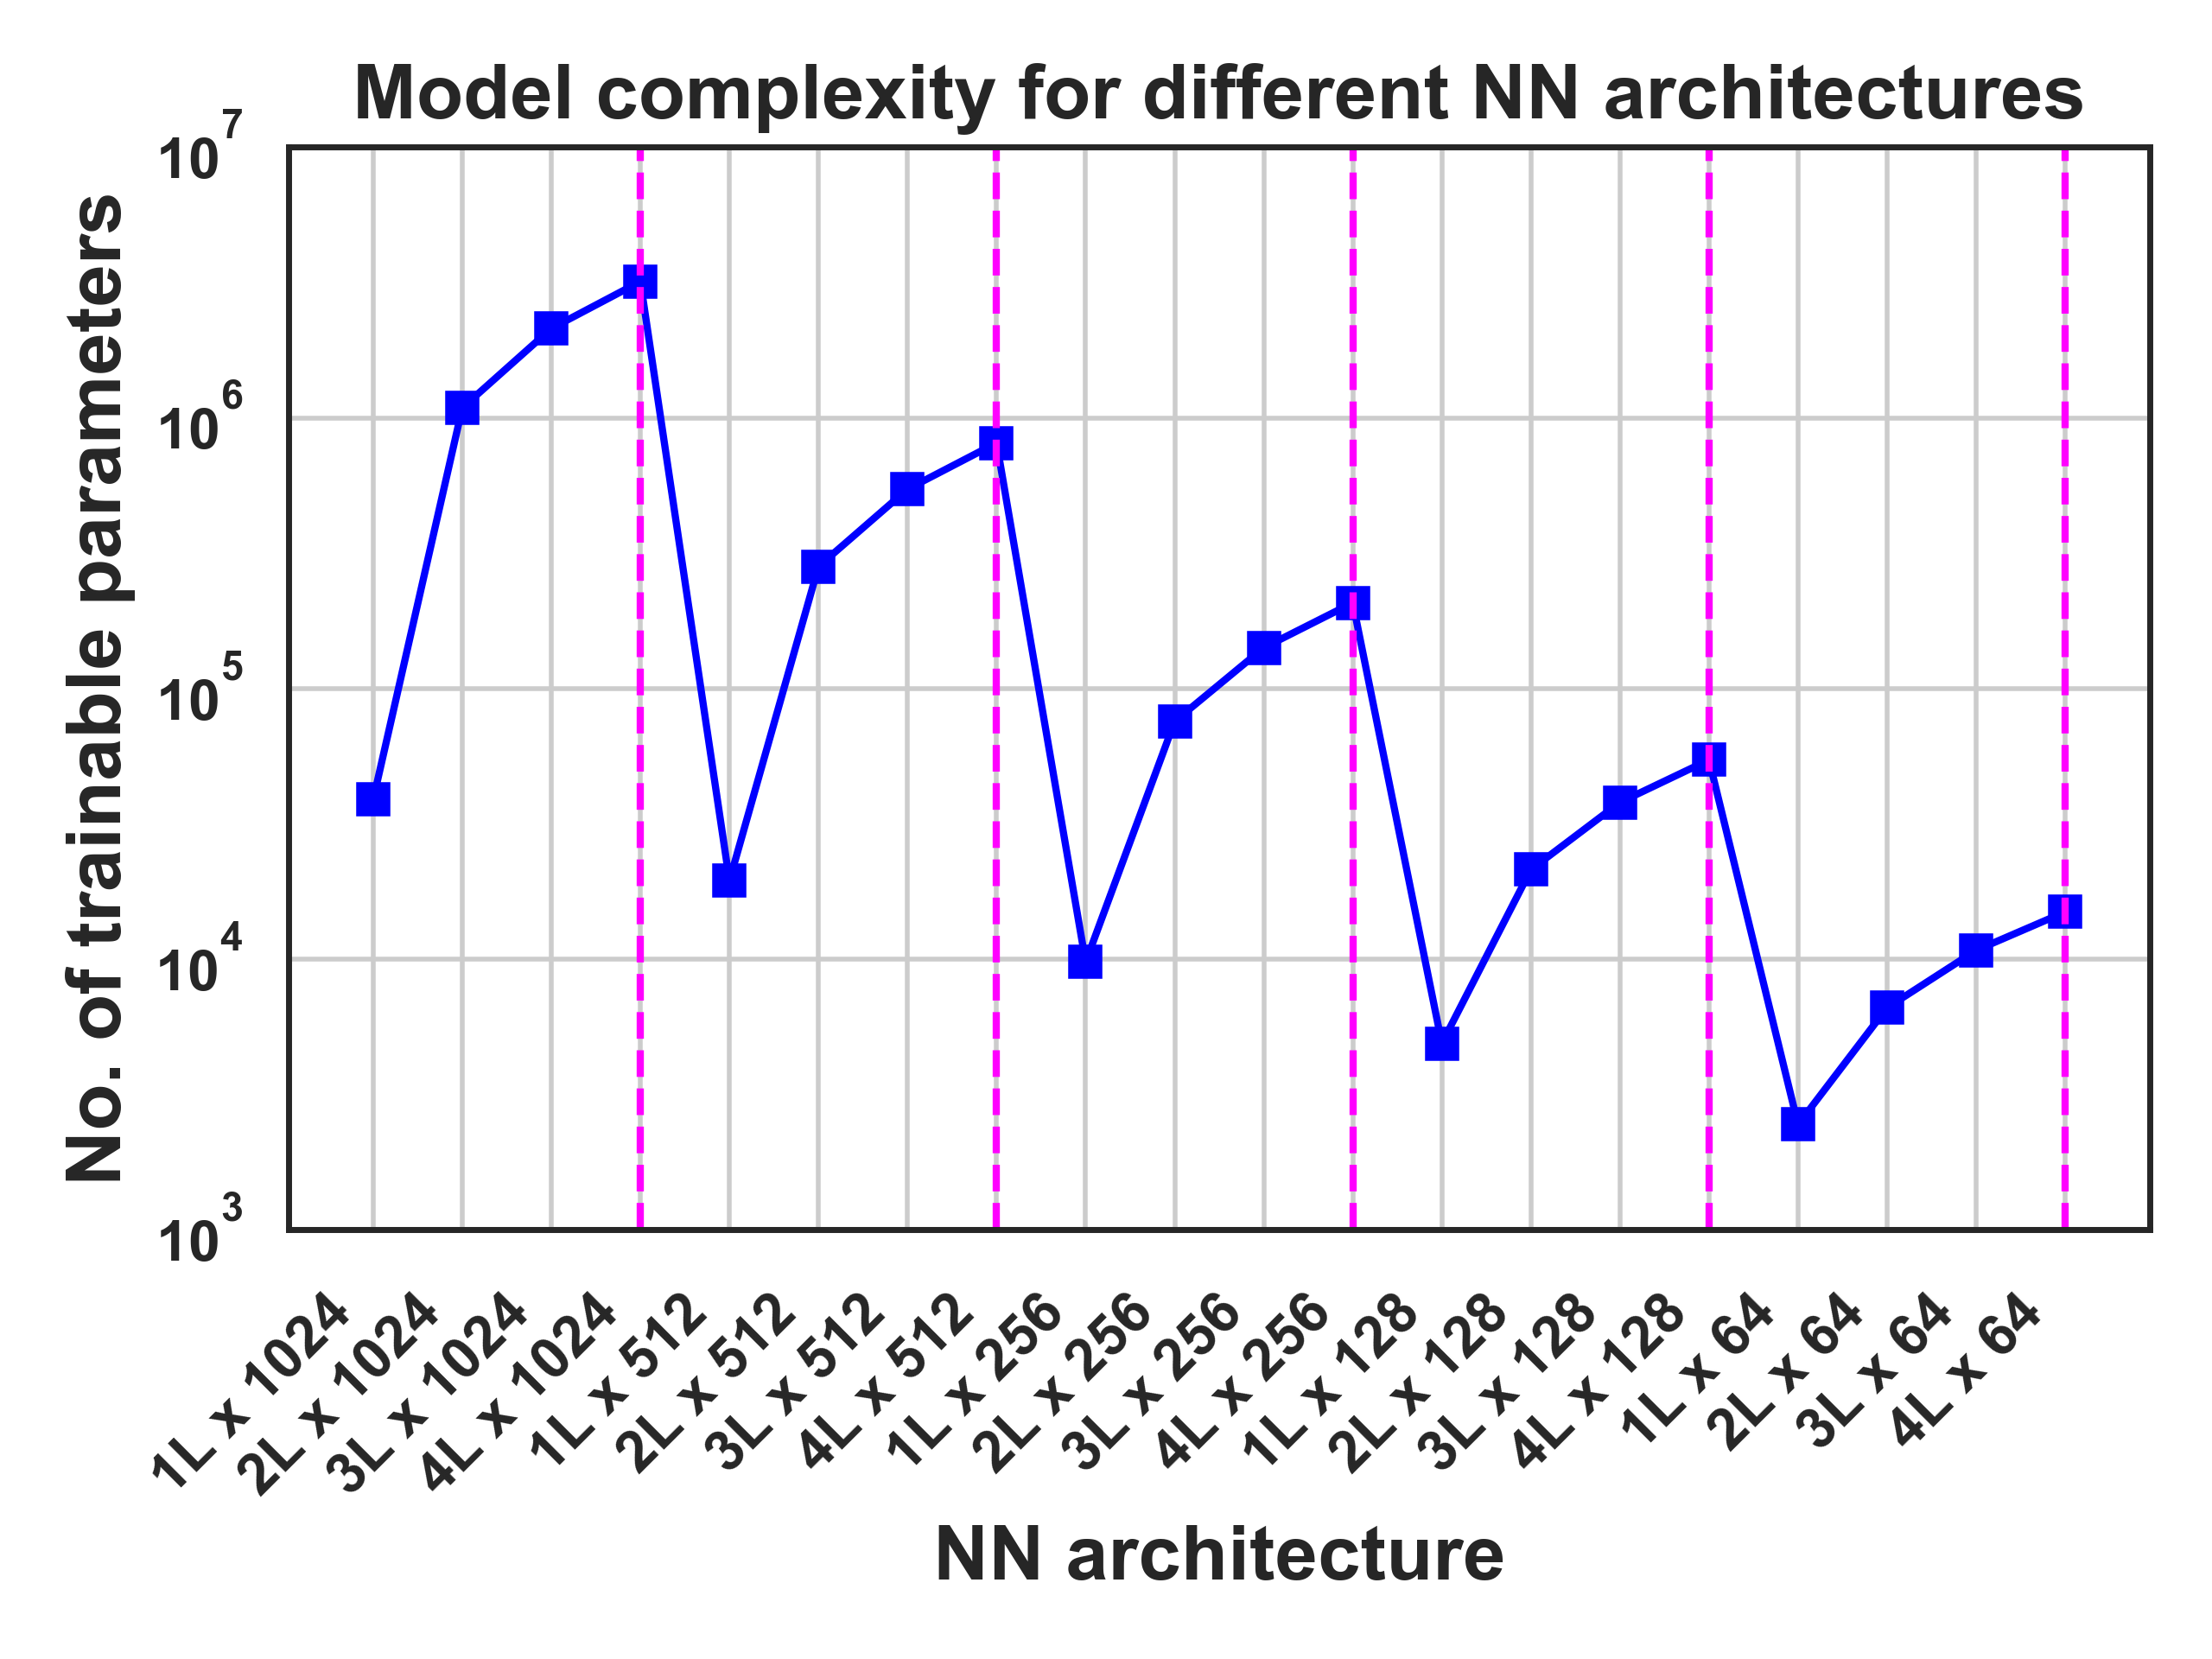
\includegraphics[width=0.48\textwidth]{Figures/Hw_num_weights_analysis_all_arch_epochs_150.png}
\caption{Line graph showing the number of trainable parameters for different FCN architectures. These parameters increase with the number of layers and neurons.}
\label{fig: weights_complexity}
\end{figure}


% \begin{figure}[ht!]
%     \captionsetup{justification=justified}
%      \centering
%      \begin{subfigure}[b]{0.48\textwidth}
%          \centering
%          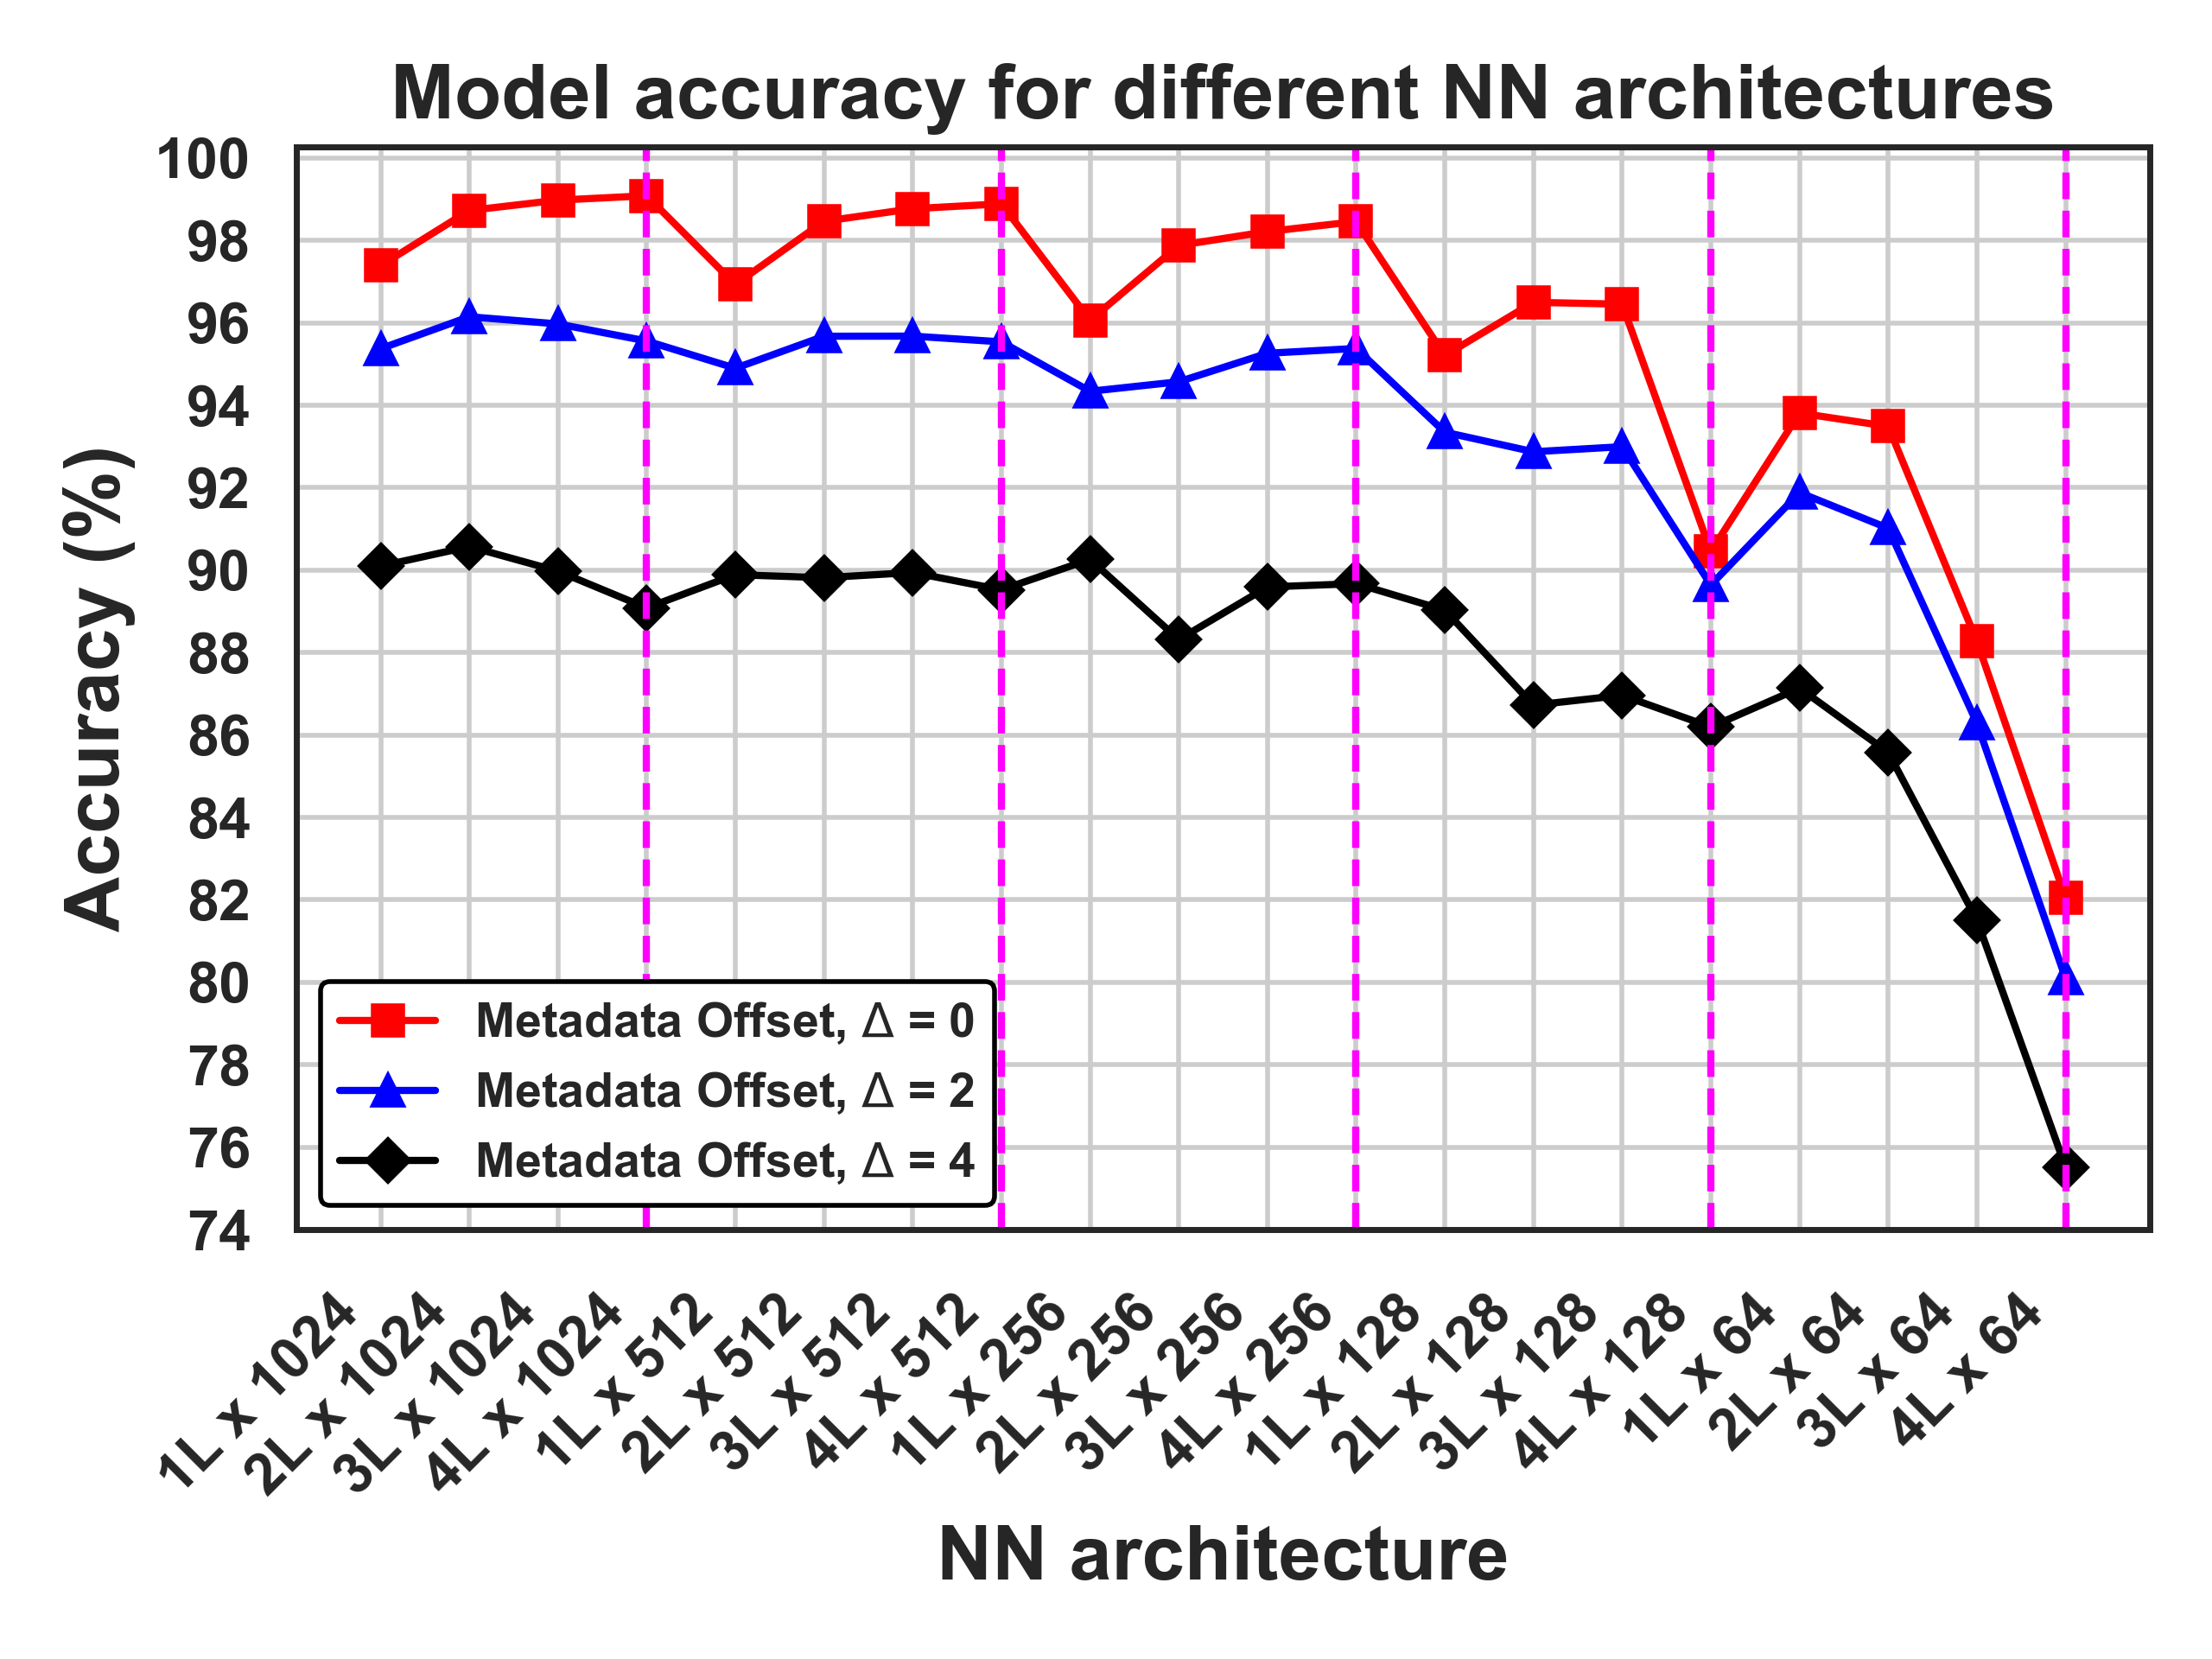
\includegraphics[width=\textwidth]{Figures/Hw_complexity_analysis_all_arch_epochs_150.png}
%          \caption{}
%          \label{fig: acc_vs_complexity}
%      \end{subfigure}
%      \\
%      \begin{subfigure}[b]{0.48\textwidth}
%          \centering
%          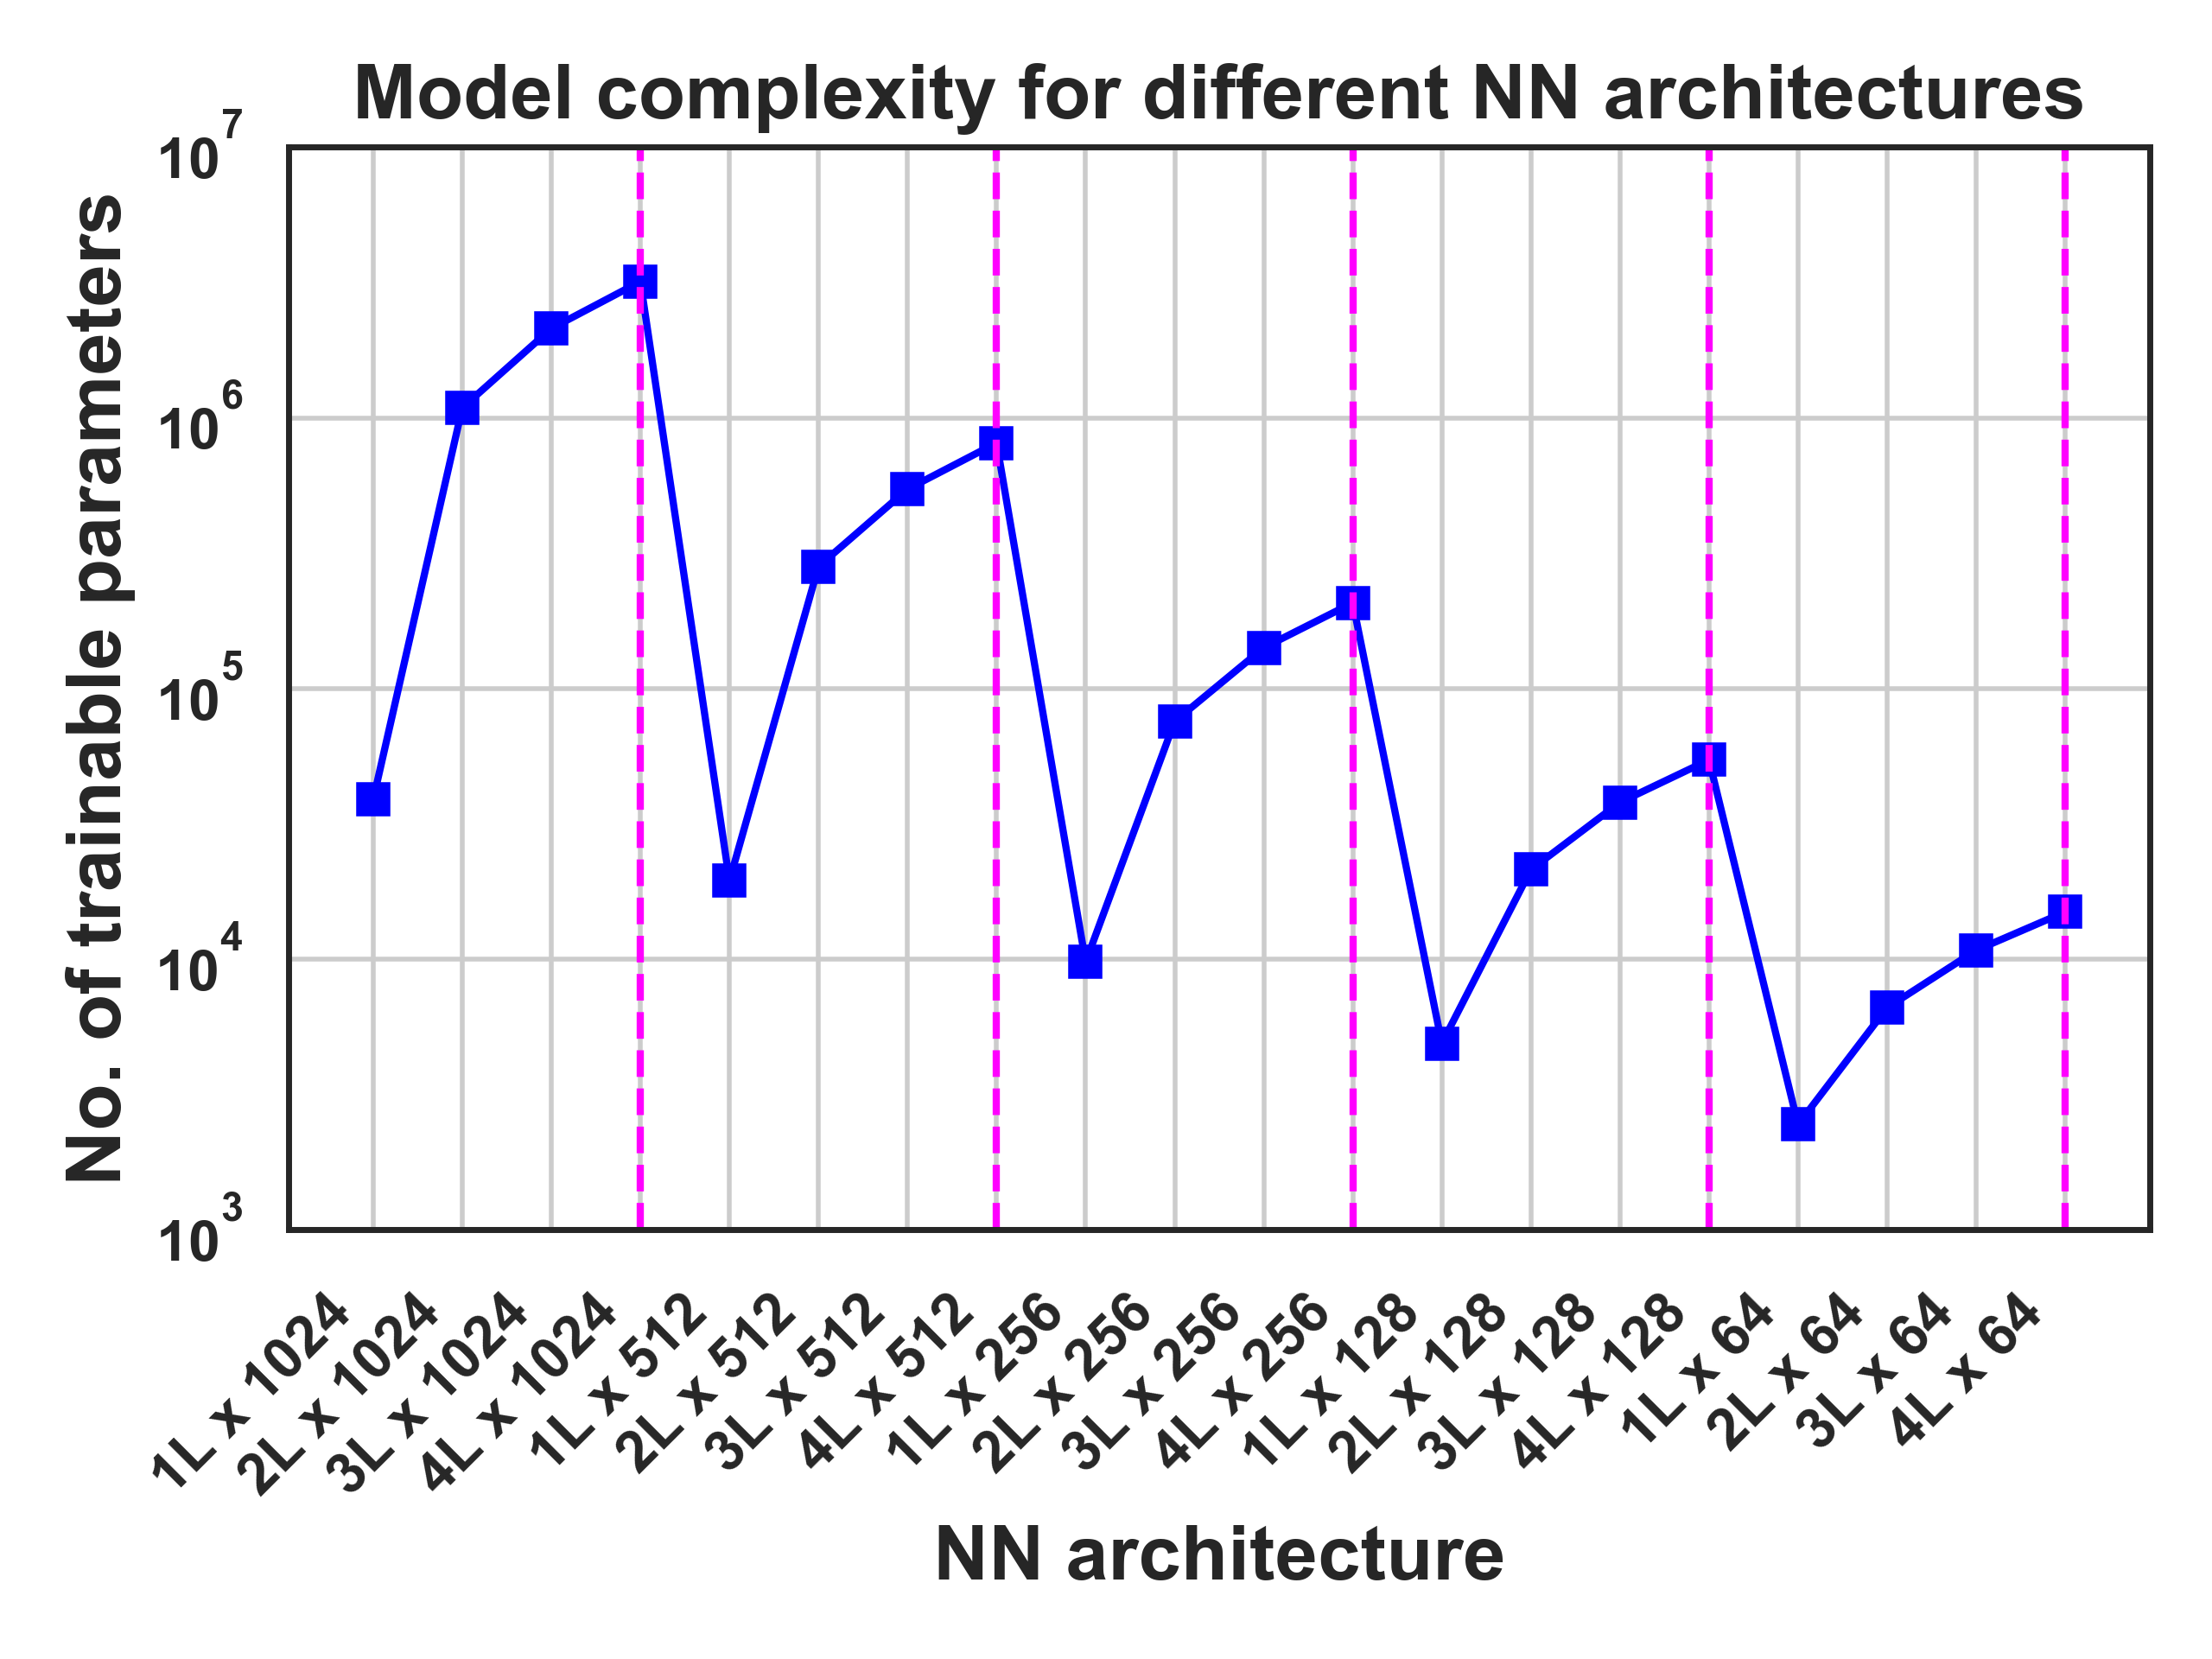
\includegraphics[width=\textwidth]{Figures/Hw_num_weights_analysis_all_arch_epochs_150.png}
%          \caption{}
%          \label{fig: weights_complexity}
%      \end{subfigure}
%         \caption{(a) Model accuracy for different FCN architectures at various values of $\Delta$, (b) Number of trainable weights for different FCN architectures}
%         \label{fig: model_complexity}
% \end{figure}


% \begin{table*}[h]
% \begin{threeparttable}
%     \caption{Hardware Complexity Analysis}
%     \centering
%     \begin{tabular}{|C{3cm}|C{2.3cm}|C{1.4cm}|C{1.4cm}|C{1.8cm}|C{1.9cm}|C{2.2cm}|}
%     % \begin{tabular}{|c|c|c|c|c|c|c|c|c|}
%         \hline
%         \textbf{NN Architecture} & \textbf{Datatype} & \textbf{Training Data size} & \textbf{Testing Data size} & \textbf{AL/ML Model Performance} & \textbf{Model Complexity} & \textbf{Computational Complexity} \\ 
%         \hline
%         \hline
%         \textbf{FCN (24,512,512,512,12)} &  &  & &  & & \\
%         \hline
%         \textbf{1} &  &  & &  & & \\
%         \hline
%         \textbf{2} &  &  & &  & & \\
%         \hline
%         \textbf{3} &  &  & &  & & \\
%         \hline
%         \textbf{4} &  &  & &  & & \\
%         \hline
%     \end{tabular}
%     \begin{tablenotes}
%     \item[1] 
%   \end{tablenotes}
%     \label{tab: hw_complexity_table}
% \end{threeparttable}
% \end{table*}

% \section*{APPENDIX}
% Appendixes, if needed, appear before the acknowledgment.

\section*{Conclusion}

In this paper, we have designed a generalized Machine Learning based PUCCH Format 0 receiver that decodes all the combinations of UCI bits across several multiplexed users. The proposed UCINet0 model is a multi-label classifier that showed superior performance compared to conventional correlation-based approaches by a significant margin. The inclusion of field datasets in the testing of the model ensures robustness and the ability of the network to work in a wide range of scenarios. In addition to standard AI/ML metrics like accuracy, we have also provided insights into the interpretability of the NN model through confusion matrices and column charts of detection percentages of individual classes.


\section*{Acknowledgment}
The authors would like to thank the Department of Telecommunications (DOT), India for funding the 5G Testbed project and the Ministry of Electronics and Information Technology (MeitY) for funding this work through the project "Next Generation Wireless Research and Standardization on 5G and Beyond".

% \section*{REFERENCES}

\bibliographystyle{IEEEtran}
% argument is your BibTeX string definitions and bibliography database(s)
\bibliography{bibfile}

\newpage

% \begin{IEEEbiography}[{\includegraphics[width=1in,height=1.25in,clip,keepaspectratio]{a1.png}}]
% {FIRST A. AUTHOR}~(Fellow, IEEE)~and all authors may include biographies.
% Biographies are often not included in conference-related papers. This author
% is an IEEE Fellow. The first paragraph may contain a place and/or date of
% birth (list place, then date). Next, the author's educational background is
% listed. The degrees should be listed with type of degree in what field,
% which institution, city, state, and country, and year the degree was earned.
% The author's major field of study should be lower-cased.

% The second paragraph uses the pronoun of the person (he or she) and not the
% author's last name. It lists military and work experience, including summer
% and fellowship jobs. Job titles are capitalized. The current job must have a
% location; previous positions may be listed without one. Information
% concerning previous publications may be included. Try not to list more than
% three books or published articles. The format for listing publishers of a
% book within the biography is: title of book (publisher name, year) similar
% to a reference. Current and previous research interests end the paragraph.

% The third paragraph begins with the author's title and last name
% (e.g., Dr.\ Smith, Prof.\ Jones, Mr.\ Kajor, Ms.\ Hunter). List any memberships in
% professional societies other than the IEEE. Finally, list any awards and
% work for IEEE committees and publications. If a photograph is provided, it
% should be of good quality, and professional-looking.
% \end{IEEEbiography}


% \begin{IEEEbiographynophoto}
% {SECOND B. AUTHOR,} photograph and biography not available at the time
% of publication.
% \end{IEEEbiographynophoto}


% \begin{IEEEbiographynophoto}
% {THIRD C. AUTHOR JR.}~(Member, IEEE), photograph and biography not available
% at the time of publication.
% \end{IEEEbiographynophoto}

\vfill\pagebreak

\end{document}

